\section{Group -- Plant Equipment}\label{group-plant-equipment}

\subsection{Equipment Types}\label{equipment-types-000}

In each \textbf{PlantEquipmentList} described using the above syntax, various equipment types and names must be given. Each type-name pair must then have a corresponding equipment definition. This subsection lists the various equipment types that are available and examples from an IDF. Where appropriate, notes and comments on the input structure are provided.

\subsection{Generic Chiller Outputs}\label{generic-chiller-outputs}

Many output variable names are common across all chiller types. These generic chiller output names all begin with the word ``Chiller''. Certain chiller types have additional output variables which are specific to that type of chiller. Chiller energy use is added to the appropriate plant-level meters as a cooling end-use.

\begin{itemize}
\item
  HVAC,Average,Chiller Electric Power {[}W{]}
\item
  HVAC,Sum,Chiller Electric Energy {[}J{]}
\item
  Zone,Meter,Electricity:Plant {[}J{]}
\item
  Zone,Meter,Cooling:Electricity {[}J{]}
\item
  HVAC,Average,Chiller Evaporator Cooling Rate {[}W{]}
\item
  HVAC,Sum,Chiller Evaporator Cooling Energy {[}J{]}
\item
  Zone,Meter,EnergyTransfer:Plant {[}J{]}
\item
  Zone,Meter,Chillers:EnergyTransfer {[}J{]}
\item
  HVAC,Average,Chiller Evaporator Inlet Temperature {[}C{]}
\item
  HVAC,Average,Chiller Evaporator Outlet Temperature {[}C{]}
\item
  HVAC,Average,Chiller Evaporator Mass Flow Rate {[}kg/s{]}
\item
  HVAC,Average,Chiller Condenser Heat Transfer Rate {[}W{]}
\item
  HVAC,Sum,Chiller Condenser Heat Transfer Energy {[}J{]}
\item
  Zone,Meter,HeatRejection:EnergyTransfer {[}J{]}
\item
  HVAC,Average,Chiller COP {[}W/W{]}
\end{itemize}

The following output is applicable only for air-cooled or evap-cooled chillers

\begin{itemize}
\tightlist
\item
  HVAC,Average,Chiller Condenser Inlet Temperature {[}C{]}
\end{itemize}

The following outputs are applicable only for evap-cooled chillers

\begin{itemize}
\item
  HVAC,Average,Chiller Basin Heater Electric Power {[}W{]}
\item
  HVAC,Average,Chiller Basin Heater Electric Energy {[}J{]}
\end{itemize}

The following three outputs are only available for water-cooled chillers

\begin{itemize}
\item
  HVAC,Average,Chiller Condenser Inlet Temperature {[}C{]}
\item
  HVAC,Average,Chiller Condenser Outlet Temperature {[}C{]}
\item
  HVAC,Average,Chiller Condenser Mass Flow Rate {[}kg/s{]}
\item
  HVAC,Average,Chiller Drive Shaft Power {[}W{]}
\item
  HVAC,Sum,Chiller Drive Shaft Energy {[}J{]}
\item
  Zone,Meter,HeatRecovery:EnergyTransfer {[}J{]}
\item
  HVAC,Average,Chiller Lube Recovered Heat Rate {[}W{]}
\item
  HVAC,Sum,Chiller Lube Recovered Heat Energy {[}J{]}
\item
  HVAC,Average,Chiller Jacket Recovered Heat Rate {[}W{]}
\item
  HVAC,Sum,Chiller Jacket Recovered Heat Energy {[}J{]}
\item
  HVAC,Average, Chiller Exhaust Recovered Heat Rate {[}W{]}
\item
  HVAC,Sum,Chiller Exhaust Recovered Heat Energy {[}J{]}
\item
  HVAC,Average,Chiller Total Recovered Heat Rate {[}W{]}
\item
  HVAC,Sum,Chiller Total Recovered Heat Energy {[}J{]}
\item
  HVAC,Average,Chiller Exhaust Temperature {[}C{]}
\item
  HVAC,Average,Chiller Heat Recovery Inlet Temperature {[}C{]}
\item
  HVAC,Average,Chiller Heat Recovery Outlet Temperature {[}C{]}
\item
  HVAC,Average,Chiller Heat Recovery Mass Flow Rate {[}kg/s{]}
\item
  HVAC,Average,Chiller Effective Heat Rejection Temperature {[}C{]}
\end{itemize}

The following blocks of outputs are for steam and fuel-driven chillers

\begin{itemize}
\item
  HVAC,Average,Chiller Gas Rate {[}W{]}
\item
  HVAC,Sum,Chiller Gas Energy {[}J{]}
\item
  HVAC,Average,Chiller Gas Mass Flow Rate {[}kg/s{]}
\item
  HVAC,Sum,Chiller Gas Mass {[}kg{]}
\end{itemize}

For steam absorption chillers:

\begin{itemize}
\item
  HVAC,Average,Chiller Source Steam Rate {[}W{]}
\item
  HVAC,Sum, Chiller Source Steam Energy {[}J{]}
\item
  HVAC,Average,Chiller Steam Mass Flow Rate {[}kg/s{]}
\end{itemize}

For hot water absorption chillers:

\begin{itemize}
\item
  HVAC,Average,Chiller Source Hot Water Rate {[}W{]}
\item
  HVAC,Sum,Chiller Source Hot Water Energy {[}J{]}
\item
  Zone,Meter,Steam:Plant {[}J{]}
\item
  Zone,Meter,Cooling:EnergyTransfer {[}J{]}
\item
  HVAC,Average,Chiller Hot Water Mass Flow Rate {[}kg/s{]}
\end{itemize}

The following output is applicable only for indirect absorption chillersHVAC,Average,Chiller Part Load Ratio

\begin{itemize}
\item
  HVAC,Average,Chiller Cycling Ratio {[]}
\item
  HVAC,Average,Chiller Propane Rate {[}W{]}
\item
  HVAC,Sum,Chiller Propane Energy {[}J{]}
\item
  HVAC,Average,Chiller Propane Mass Flow Rate {[}kg/s{]}
\item
  HVAC,Average,Chiller Diesel Rate {[}W{]}
\item
  HVAC,Sum,Chiller Diesel Energy {[}J{]}
\item
  HVAC,Average,Chiller Diesel Mass Flow Rate {[}kg/s{]}
\item
  HVAC,Average,Chiller Gasoline Rate {[}W{]}
\item
  HVAC,Sum,Chiller Gasoline Energy {[}J{]}
\item
  HVAC,Average,Chiller Gasoline Mass Flow Rate {[}kg/s{]}
\item
  HVAC,Average,Chiller FuelOil\#1 Rate {[}W{]}
\item
  HVAC,Sum,Chiller FuelOil\#1 Energy {[}J{]}
\item
  HVAC,Average,Chiller FuelOil\#1 Mass Flow Rate {[}kg/s{]}
\item
  HVAC,Average,Chiller FuelOil\#2 Rate {[}W{]}
\item
  HVAC,Sum,Chiller FuelOil\#2 Energy {[}J{]}
\item
  HVAC,Average,Chiller FuelOil\#2 Mass Flow Rate {[}kg/s{]}
\item
  HVAC,Average,Chiller OtherFuel1 Rate {[}W{]}
\item
  HVAC,Sum,Chiller OtherFuel1 Energy {[}J{]}
\item
  HVAC,Average,Chiller OtherFuel1 Mass Flow Rate {[}kg/s{]}
\item
  HVAC,Average,Chiller OtherFuel2 Rate {[}W{]}
\item
  HVAC,Sum,Chiller OtherFuel2 Energy {[}J{]}
\item
  HVAC,Average,Chiller OtherFuel2 Mass Flow Rate {[}kg/s{]}
\end{itemize}

\subsubsection{Chiller Electric Power {[}W{]}}\label{chiller-electric-power-w}

\subsubsection{Chiller Electric Energy {[}J{]}}\label{chiller-electric-energy-j}

These outputs are the electric power input to the chiller. In the case of steam or fuel-powered chillers, this repesents the internal chiller pumps and other electric power consumption. Consumption is metered on Cooling:Electricity, Electricity:Plant, and Electricity:Facility.

\subsubsection{Chiller Evaporator Cooling Rate {[}W{]}}\label{chiller-evaporator-cooling-rate-w}

\subsubsection{Chiller Evaporator Cooling Energy {[}J{]}}\label{chiller-evaporator-cooling-energy-j}

These outputs are the evaporator heat transfer which is the cooling delivered by the chiller. Chiller Evaporator Cooling Energy is metered on Chillers:EnergyTransfer, EnergyTransfer:Plant, and EnergyTransfer:Facility.

\subsubsection{Chiller Evaporator Inlet Temperature {[}C{]}}\label{chiller-evaporator-inlet-temperature-c}

\subsubsection{Chiller Evaporator Outlet Temperature {[}C{]}}\label{chiller-evaporator-outlet-temperature-c}

\subsubsection{Chiller Evaporator Mass Flow Rate {[}kg/s{]}}\label{chiller-evaporator-mass-flow-rate-kgs}

These outputs are the evaporator (chilled water) inlet and outlet temperatures and flow rate.

\subsubsection{Chiller COP {[}W/W{]}}\label{chiller-cop-ww}

This output is the coefficient of performance for the chiller during cooling operation. It is calculated as the evaporator heat transfer rate (Chiller Evaporator Cooling Rate) divided by the ``fuel'' consumption rate by the chiller. For the constant COP and electric chillers, the ``fuel'' is electricity so the divisor is Chiller Electric Power {[}W{]}. For the absorption chiller, the ``fuel'' is steam so the divisor is Steam Consumption Rate {[}W{]}.

\emph{Note that this variable is reported as zero when the chiller is not operating. When reported for frequencies longer than ``detailed'' (such as timestep, hourly, daily, monthly or environment), this output will only be meaningful when the chiller is operating for the entire reporting period. To determine an average COP for a longer time period, compute the COP based on total evaporator heat transfer divided by total electric or fuel input over the desired period.}

\subsubsection{Chiller Part Load Ratio}\label{chiller-part-load-ratio}

This output is the operating part-load ratio of the indirect absorption chiller. This output may fall below the minimum part-load ratio specified in the input. For this case, the Chiller Cycling Ratio is used to further define the performance of the indirect absorption chiller.

\subsubsection{Chiller Cycling Ratio}\label{chiller-cycling-ratio}

This output is the fraction of the timestep the indirect absorption chiller operates. When the chiller operates above the minimum part-load ratio, a Chiller Cycling Ratio of 1 is reported. When the chiller operates below the minimum part-load ratio, the Chiller Cycling Ratio reports the fraction of the timestep the indirect absorption chiller operates.

\subsubsection{Chiller Condenser Heat Transfer Rate {[}W{]}}\label{chiller-condenser-heat-transfer-rate-w}

\subsubsection{Chiller Condenser Heat Transfer Energy {[}J{]}}\label{chiller-condenser-heat-transfer-energy-j}

These outputs are the condenser heat transfer which is the heat rejected from the chiller to either a condenser water loop or through an air-cooled condenser. Chiller Condenser Heat Transfer Energy is metered on HeatRejection:EnergyTransfer, EnergyTransfer:Plant, and EnergyTransfer:Facility.

\subsubsection{Chiller Condenser Inlet Temperature {[}C{]}}\label{chiller-condenser-inlet-temperature-c}

This output is the condenser (heat rejection) inlet temperature for air-cooled or evap-cooled chillers. For an air-cooled chiller, this output would be the dry-bulb temperature of the air entering the condenser coil. For an evap-cooled chiller, this output would be the wet-bulb temperature of the air entering the evaporatively-cooled condenser coil.

\subsubsection{Chiller Basin Heater Electric Power {[}W{]}}\label{chiller-basin-heater-electric-power-w}

\subsubsection{Chiller Basin Heater Electric Energy {[}J{]}}\label{chiller-basin-heater-electric-energy-j}

These outputs are the electric power input to the chiller's basin heater (for evaporatively-cooled condenser type). Consumption is metered on Chillers:Electricity, Electricity:Plant, and Electricity:Facility

\subsubsection{Chiller Condenser Inlet Temperature {[}C{]}}\label{chiller-condenser-inlet-temperature-c-1}

\subsubsection{Chiller Condenser Outlet Temperature {[}C{]}}\label{chiller-condenser-outlet-temperature-c}

\subsubsection{Chiller Condenser Mass Flow Rate {[}kg/s{]}}\label{chiller-condenser-mass-flow-rate-kgs}

These outputs are the condenser (heat rejection) inlet and outlet temperatures and flow rate for water-cooled chillers.

\subsubsection{Chiller Drive Shaft Power {[}W{]}}\label{chiller-drive-shaft-power-w}

\subsubsection{Chiller Drive Shaft Energy {[}J{]}}\label{chiller-drive-shaft-energy-j}

For engine-driven and turbine-driven chillers, these outputs are the shaft power produced by the prime mover and transferred to the chiller compressor.

\subsubsection{Chiller Lube Recovered Heat Rate {[}W{]}}\label{chiller-lube-recovered-heat-rate-w}

\subsubsection{Chiller Lube Recovered Heat Energy {[}J{]}}\label{chiller-lube-recovered-heat-energy-j}

\subsubsection{Chiller Jacket Recovered Heat Rate {[}W{]}}\label{chiller-jacket-recovered-heat-rate-w}

\subsubsection{Chiller Jacket Recovered Heat Energy {[}J{]}}\label{chiller-jacket-recovered-heat-energy-j}

\subsubsection{Chiller Exhaust Recovered Heat Rate {[}W{]}}\label{chiller-exhaust-recovered-heat-rate-w}

\subsubsection{Chiller Exhaust Recovered Heat Energy {[}J{]}}\label{chiller-exhaust-recovered-heat-energy-j}

\subsubsection{Chiller Total Recovered Heat Rate {[}W{]}}\label{chiller-total-recovered-heat-rate-w}

\subsubsection{Chiller Total Recovered Heat Energy {[}J{]}}\label{chiller-total-recovered-heat-energy-j}

For chillers with heat recovery, such as engine-driven chillers, these outputs are the components of recoverable energy available. For a given chiller type, one or more of the following components may be applicable:~ Lube (engine lubricant), Jacket (engine coolant), Exhaust (engine exhaust), and Total. Chiller Lube Recovered Heat Energy, Chiller Jacket Recovered Heat Energy, and Chiller Exhaust Heat Recovery Energy are metered on HeatRecovery:EnergyTransfer, EnergyTransfer:Plant, and EnergyTransfer:Facility.

\subsubsection{Chiller Exhaust Temperature {[}C{]}}\label{chiller-exhaust-temperature-c}

This is the exhaust temperature leaving an engine chiller.

\subsubsection{Chiller Heat Recovery Inlet Temperature {[}C{]}}\label{chiller-heat-recovery-inlet-temperature-c}

\subsubsection{Chiller Heat Recovery Outlet Temperature {[}C{]}}\label{chiller-heat-recovery-outlet-temperature-c}

\subsubsection{Chiller Heat Recovery Mass Flow Rate {[}kg/s{]}}\label{chiller-heat-recovery-mass-flow-rate-kgs}

These outputs are the heat recovery inlet and outlet temperatures and flow rate for chillers with heat recovery such as engine-driven and gas turbine chillers.

\subsubsection{Chiller Effective Heat Rejection Temperature {[}C{]}}\label{chiller-effective-heat-rejection-temperature-c}

This output variable is available for heat recovery chillers that model split bundle condenser.~ The condenser fluid temperatures used to characterize chiller performance are modified to account for the temperature of the heat recovery fluid.~ This output is the resulting temperature used for characterizing chiller performance and is a blend of the temperatures in the condenser and heat recovery fluid streams.~ For the Chiller:Electric and Chiller:Electric:EIR models, this is an effective inlet temperature while for the Chiller:Electric:ReformulatedEIR model, this is an effective outlet temperature.

\subsubsection{Chiller \textless{}Fuel Type\textgreater{} Rate {[}W{]}}\label{chiller-fuel-type-rate-w}

\subsubsection{Chiller \textless{}Fuel Type\textgreater{} Energy~ {[}J{]}}\label{chiller-fuel-type-energy-j}

\subsubsection{Chiller~ \textless{}Fuel Type\textgreater{} Mass Flow Rate {[}kg/s{]}}\label{chiller-fuel-type-mass-flow-rate-kgs}

\subsubsection{Chiller Gas~ Mass {[}kg{]} (Gas Turbine Chiller only)}\label{chiller-gas-mass-kg-gas-turbine-chiller-only}

These outputs are the steam or fuel input for steam or fuel-fired chillers. Valid fuel types depend on the type of chiller. \textless{}Fuel Type\textgreater{} may be one of:~ Gas (natural gas), Steam, Propane, Diesel, Gasoline, FuelOil\#1, FuelOil\#2, OtherFuel1 and OtherFuel2. Consumption is metered on Cooling:\textless{}Fuel Type\textgreater{}, \textless{}Fuel Type\textgreater{}:Plant, and \textless{}Fuel Type\textgreater{}:Facility.

\subsubsection{Chiller Source Hot Water Rate {[}W{]}}\label{chiller-source-hot-water-rate-w}

\subsubsection{Chiller Source Hot Water Energy {[}J{]}}\label{chiller-source-hot-water-energy-j}

\subsubsection{Chiller Source Steam Rate {[}W{]}}\label{chiller-source-steam-rate-w}

\subsection{Chiller:Absorption}\label{chillerabsorption}

\subsubsection{Inputs}\label{inputs-036}

\paragraph{Field: Name}\label{field-name-035}

This alpha field contains the identifying name for the absorption chiller.

\paragraph{Field: Nominal Capacity}\label{field-nominal-capacity-001}

This numeric field contains the nominal cooling capability of the chiller in Watts.

\paragraph{Field: Nominal Pumping Power}\label{field-nominal-pumping-power}

This numeric field contains the nominal pumping power of the absorber in Watts.

\paragraph{Field: Chilled Water Inlet Node Name}\label{field-chilled-water-inlet-node-name-000}

This required alpha field contains the identifying name for the absorption chiller plant side inlet node.

\paragraph{Field: Chilled Water Outlet Node Name}\label{field-chilled-water-outlet-node-name-000}

This required alpha field contains the identifying name for the absorption chiller plant side outlet node.

\paragraph{Field: Condenser Inlet Node Name}\label{field-condenser-inlet-node-name}

This required alpha field contains the identifying name for the absorption chiller condenser side inlet node.

\paragraph{Field: Condenser Outlet Node Name}\label{field-condenser-outlet-node-name}

This required alpha field contains the identifying name given to the Heat Recovery Loop Component Outlet Node.

\paragraph{Field: Minimum Part Load Ratio}\label{field-minimum-part-load-ratio-001}

This numeric field contains the absorption chiller's minimum part load ratio. The expected range is between 0 and 1. The minimum part load is not the load where the machine shuts off, but where the amount of power remains constant to produce smaller loads than this fraction.

\paragraph{Field: Maximum Part Load Ratio}\label{field-maximum-part-load-ratio-001}

This numeric field contains the absorption chiller's maximum part load ratio. This value may exceed 1, but the normal range is between 0 and 1.1.

\paragraph{Field: Optimum Part Load Ratio}\label{field-optimum-part-load-ratio-001}

This numeric field contains the absorption chiller's optimum part load ratio. This is the part load ratio at which the chiller performs at its maximum COP.

\paragraph{Field: Design Condenser Inlet Temperature}\label{field-design-condenser-inlet-temperature}

This numeric field contains the absorption chiller's condenser inlet design temperature in Celsius.

\paragraph{Field: Design Chilled Water Flow Rate}\label{field-design-chilled-water-flow-rate}

For variable volume chiller this is the maximum flow and for constant flow chiller this is the design flow rate. The units are in cubic meters per second.

\paragraph{Field: Design Condenser Water Flow Rate}\label{field-design-condenser-water-flow-rate}

This numeric field contains the absorption chiller's design condenser water flow rate in cubic meters per second.

\paragraph{Generator Heat Input Part Load Ratio Curve}\label{generator-heat-input-part-load-ratio-curve}

The Generator Heat Input Part Load Ratio Curve is a quadratic equation that determines the Ratio of the generator load on the absorber to the demand on the chiller. The defining equation is:

\begin{equation}
SteamInputRatio = \frac{{C1}}{{PLR}} + C2 + C3 * PLR
\end{equation}

The following three fields contain the coefficients for the equation.

\paragraph{Field: Coefficient 1 of the Steam Use Part Load Ratio Curve}\label{field-coefficient-1-of-the-steam-use-part-load-ratio-curve}

C1 in the Generator Heat Input Part Load Ratio Curve. This value is obtained by fitting manufacturers' performance data to the curve.

\paragraph{Field: Coefficient 2 of the Steam Use Part Load Ratio Curve}\label{field-coefficient-2-of-the-steam-use-part-load-ratio-curve}

C2 in the Generator Heat Input Part Load Ratio Curve. This value is obtained by fitting manufacturers' performance data to the curve.

\paragraph{Field: Coefficient 3 of the Steam Use Part Load Ratio Curve}\label{field-coefficient-3-of-the-steam-use-part-load-ratio-curve}

C3 in the Generator Heat Input Part Load Ratio Curve. This value is obtained by fitting manufacturers' performance data to the curve.

\paragraph{Pump Electric Use Part Load Ratio Curve}\label{pump-electric-use-part-load-ratio-curve}

The Pump Electric Use Part Load Ratio Curve is a quadratic equation that determines the Ratio of~ the actual absorber pumping power to the nominal pumping power. The defining equation is:

\begin{equation}
ElectricInputRatio = C1 + C2 * PLR + C3 * PL{R^2}
\end{equation}

The following three fields contain the coefficients for the equation.

\paragraph{Field: Coefficient 1 of the Pump Electric Use Part Load Ratio Curve}\label{field-coefficient-1-of-the-pump-electric-use-part-load-ratio-curve}

C1 in the Pump Electric Use Part Load Ratio Curve. This value is obtained by fitting manufacturers' performance data to the curve.

\paragraph{Field: Coefficient 2 of the Pump Electric Use Part Load Ratio Curve}\label{field-coefficient-2-of-the-pump-electric-use-part-load-ratio-curve}

C2 in the Pump Electric Use Part Load Ratio Curve. This value is obtained by fitting manufacturers' performance data to the curve.

\paragraph{Field: Coefficient 3 of the Pump Electric Use Part Load Ratio Curve}\label{field-coefficient-3-of-the-pump-electric-use-part-load-ratio-curve}

C3 in the Pump Electric Use Part Load Ratio Curve. This value is obtained by fitting manufacturers' performance data to the curve.

\paragraph{Field: Chilled Water Outlet Temperature Lower Limit}\label{field-chilled-water-outlet-temperature-lower-limit}

This numeric field contains the lower limit for the evaporator outlet temperature. This temperature acts as a cut off for heat transfer in the evaporator, so that the fluid doesn't get too cold.

\paragraph{Field: Generator Inlet Node Name}\label{field-generator-inlet-node-name}

This alpha field contains the identifying name given to the Generator Inlet Node. A steam or hot water loop is not required to simulate an absorption chiller. If a steam/hot water loop is used, enter the name of the generator inlet node.

\paragraph{Field: Generator Outlet Node Name}\label{field-generator-outlet-node-name}

This alpha field contains the identifying name given to the Generator Outlet Node. A steam or hot water loop is not required to simulate an absorption chiller. If a steam/hot water loop is used, enter the name of the generator outlet node.

\paragraph{Field: Chiller Flow Mode}\label{field-chiller-flow-mode}

This choice field determines how the chiller operates with respect to the intended fluid flow through the device's evaporator. ~There are three different choices for specifying operating modes for the intended flow behavior:~ ``NotModulated,'' ``ConstantFlow,'' and ``LeavingSetpointModulated.''~ NotModulated is useful for either variable or constant speed pumping arrangements where the chiller is passive in the sense that although it makes a nominal request for its design flow rate it can operate at varying flow rates.~ ConstantFlow is useful for constant speed pumping arrangements where the chiller's request for flow is stricter and can increase the overall loop flow.~ LeavingSetpointModulated changes the chiller model to internally vary the flow rate so that the temperature leaving the chiller matches a setpoint at the evaporator outlet.~ For this absorption chiller, this mode also affects the flow rate on the generator connection.~ In all cases the operation of the external plant system can also impact the flow through the chiller -- for example if the relative sizes and operation are such that flow is restricted and the requests cannot be met.~ The default, if not specified, is NotModulated.~ This flow mode does not impact the condenser loop connection.

\paragraph{Field: Generator Fluid Type}\label{field-generator-fluid-type}

This choice field specifies the type of fluid used to heat the generator solution. The valid choices are \textbf{HotWater} or \textbf{Steam}. This field should be specified as Steam or left blank if the generator inlet/outlet nodes are not specified.

\paragraph{Field: Design Generator Fluid Flow Rate}\label{field-design-generator-fluid-flow-rate}

This numeric field contains the absorption chiller's design condenser fluid flow rate in cubic meters per second.

\paragraph{Field: Degree of Subcooling in Steam Generator}\label{field-degree-of-subcooling-in-steam-generator}

Ideally, the steam trap located at the outlet of the generator should remove all the condensate immediately, however, there is a delay in this process in actual systems which causes the condensate to SubCool by a certain amount before leaving the generator. This amount of subcooling is included in the heat transferred to the solution in the generator. The minimum value is 0º Celsius and default is 5º Celsius. This field is not used when the generator inlet/outlet node are not specified or the generator is connected to a hot water loop.

\paragraph{Field: Sizing Factor}\label{field-sizing-factor-001}

This optional numeric field allows the user to specify a sizing factor for this component. The sizing factor is used when the component design inputs are autosized: the autosizing calculations are performed as usual and the results are multiplied by the sizing factor. For this component the inputs that would be altered by the sizing factor are: Nominal Capacity, Nominal Pumping Power, Design Chilled Water Flow Rate, Design Condenser Water Flow Rate and Design Generator Fluid Flow Rate. Sizing factor allows the user to size a component to meet part of the design load while continuing to use the autosizing feature.

Following is an example input for an Absorption Chiller.

\begin{lstlisting}

Chiller:Absorption,
      Big Chiller,             !- Chiller Name
      50000,                   !- Nominal Capacity {W}
      250,                     !- Nominal Pumping Power {W}
      Big Chiller Inlet Node,  !- Plant_Side_Inlet_Node
      Big Chiller Outlet Node, !- Plant_Side_Outlet_Node
      Big Chiller Condenser Inlet Node,  !- Condenser_Side_Inlet_Node
      Big Chiller Condenser Outlet Node,  !- Condenser_Side_Outlet_Node
      0.15,                    !- Minimum Part Load Ratio
      1.0,                     !- Maximum Part Load Ratio
      0.65,                    !- Opt Part Load Ratio
      35.0,                    !- Temp Design Condenser Inlet {C}
      0.0011,                  !- Design Chilled Water Flow Rate {m3/s}
      0.0011,                  !- Design Condenser Water Flow Rate {m3/s}
      0.03303,                 !- Coefficient1 of the steam use part load ratio curve
      0.6852,                  !- Coefficient2 of the steam use part load ratio curve
      0.2818,                  !- Coefficient3 of the steam use part load ratio curve
      1.0,                     !- Coefficient1 of the pump electric use part load ratio curve
      0,                       !- Coefficient2 of the pump electric part load ratio curve
      0,                       !- Coefficient3 of the pump electric use part load ratio curve
      5,                       !- Chilled Water Outlet Temperature Lower Limit {C}
      AbsorberSteamInletNode,  !- Generator Inlet Node Name
      AbsorberSteamOutletNode, !- Generator Outlet Node Name
      VariableFlow,            !- Chiller Flow Mode
      Steam,                   !- Generator Fluid Type
      autosize,                !- Design Generator Volumetric Fluid Flow Rate {m3/s}
      2.0;                     !- Degree of Subcooling in Steam Generator {C}
\end{lstlisting}

\subsubsection{Outputs}\label{outputs-025}

\begin{itemize}
\item
  HVAC,Average,Chiller Electric Power {[}W{]}
\item
  HVAC,Sum,Chiller Electric Energy {[}J{]}
\item
  Zone,Meter,Electricity:Plant {[}J{]}
\item
  Zone,Meter,Cooling:Electricity {[}J{]}
\item
  HVAC,Average,Chiller Evaporator Cooling Rate {[}W{]}
\item
  HVAC,Sum,Chiller Evaporator Cooling Energy {[}J{]}
\item
  Zone,Meter,EnergyTransfer:Plant {[}J{]}
\item
  Zone,Meter,Chillers:EnergyTransfer {[}J{]}
\item
  HVAC,Average,Chiller Evaporator Inlet Temperature {[}C{]}
\item
  HVAC,Average,Chiller Evaporator Outlet Temperature {[}C{]}
\item
  HVAC,Average,Chiller Evaporator Mass Flow Rate {[}kg/s{]}
\item
  HVAC,Average,Chiller Condenser Heat Transfer Rate {[}W{]}
\item
  HVAC,Sum,Chiller Condenser Heat Transfer Energy {[}J{]}
\item
  Zone,Meter,HeatRejection:EnergyTransfer {[}J{]}
\item
  HVAC,Average,Chiller Condenser Inlet Temperature {[}C{]}
\item
  HVAC,Average,Chiller Condenser Outlet Temperature {[}C{]}
\item
  HVAC,Average,Chiller Condenser Mass Flow Rate {[}kg/s{]}
\item
  HVAC,Average,Chiller COP {[}W/W{]}
\end{itemize}

For Chillers with Steam Generators:

\begin{itemize}
\item
  HVAC,Average, Chiller Source Steam Rate {[}W{]}
\item
  HVAC,Sum, Chiller Source Steam Energy {[}J{]}
\item
  HVAC,Average,Chiller Steam Mass Flow Rate {[}kg/s{]}
\end{itemize}

For Chillers with Hot Water Generators:

\begin{itemize}
\item
  HVAC,Average,Chiller Source Hot Water Rate {[}W{]}
\item
  HVAC,Sum,Chiller Source Hot Water Energy {[}J{]}
\item
  HVAC,Average,Chiller Hot Water Mass Flow Rate {[}kg/s{]}
\end{itemize}

These chiller output variables are defined above under ``Generic Chiller Outputs.''

\subsection{Chiller:Absorption:Indirect}\label{chillerabsorptionindirect}

The Chiller:Absorption:Indirect object is an enhanced version of the absorption chiller model found in the Building Loads and System Thermodynamics (BLAST) program. This enhanced model is nearly identical to the existing absorption chiller model (Ref. Chiller:Absorption) with the exceptions that: 1) the enhanced indirect absorption chiller model provides more flexible performance curves and 2) chiller performance now includes the impact of varying evaporator, condenser, and generator temperatures. Since these absorption chiller models are nearly identical (i.e., the performance curves of the enhanced model can be manipulated to produce similar results to the previous model), it is quite probable that the Chiller:Absorption model will be deprecated in a future release of EnergyPlus.

\subsubsection{Inputs}\label{inputs-1-033}

\paragraph{Field: Name}\label{field-name-1-032}

This required alpha field contains the identifying name for the indirect absorption chiller.

\paragraph{Field: Nominal Capacity}\label{field-nominal-capacity-1-001}

This required numeric field contains the nominal cooling capability of the chiller in Watts. This field must be greater than 0 and is autosizable.

\paragraph{Field: Nominal Pumping Power}\label{field-nominal-pumping-power-1}

This required numeric field contains the nominal pumping power of the chiller in Watts. The minimum value for this field is 0 and is autosizable.

\paragraph{Field: Chilled Water Inlet Node Name}\label{field-chilled-water-inlet-node-name-1-000}

This required alpha field contains the identifying name for the chiller chilled water inlet node.

\paragraph{Field: Chilled Water Outlet Node Name}\label{field-chilled-water-outlet-node-name-1-000}

This required alpha field contains the identifying name for the chiller chilled water outlet node.

\paragraph{Field: Condenser Inlet Node Name}\label{field-condenser-inlet-node-name-1}

This required alpha field contains the identifying name for the chiller condenser inlet node.

\paragraph{Field: Condenser Outlet Node Name}\label{field-condenser-outlet-node-name-1}

This required alpha field contains the identifying name given to the chiller outlet node.

\paragraph{Field: Minimum Part Load Ratio}\label{field-minimum-part-load-ratio-1-001}

This numeric field contains the chiller's minimum part-load ratio. The expected range is between 0 and 1. The minimum part load is not the load where the machine shuts off, but where the amount of power remains constant to produce smaller loads than this fraction.

\paragraph{Field: Maximum Part Load Ratio}\label{field-maximum-part-load-ratio-1-001}

This numeric field contains the chiller's maximum part-load ratio. This value may exceed 1, but the normal range is between 0 and 1.1.

\paragraph{Field: Optimum Part Load Ratio}\label{field-optimum-part-load-ratio-1-001}

This numeric field contains the chiller's optimum part-load ratio. This is the part-load ratio at which the chiller performs at its maximum COP.

\paragraph{Field: Design Condenser Inlet Temperature}\label{field-design-condenser-inlet-temperature-1}

This numeric field contains the chiller's condenser inlet design temperature in Celsius. The default value for this field is 30º C and is only used when the Design Chilled Water Flow Rate is autosized.

\paragraph{Field: Condenser Inlet Temperature Lower Limit}\label{field-condenser-inlet-temperature-lower-limit}

This numeric field contains the chiller's lower limit for the condenser entering water temperature in Celsius. The default value for this field is 15º C. If this limit is exceeded, a warning message will report the incident. No correction to chiller capacity is made for low condenser entering water temperatures.

\paragraph{Field: Chilled Water Outlet Temperature Lower Limit}\label{field-chilled-water-outlet-temperature-lower-limit-1}

This numeric field contains the chiller's lower limit for the evaporator leaving water temperature in Celsius. The default value for this field is 5º C. If this limit is exceeded, a warning message will report the incident. No correction to chiller capacity is made for low evaporator leaving water temperatures.

\paragraph{Field: Design Chilled Water Flow Rate}\label{field-design-chilled-water-flow-rate-1}

This numeric input specifies the design evaporator volumetric flow rate in cubic meters per second. The value specified must be greater than 0 or this field is autosizable. For variable volume chiller this is the maximum flow and for constant flow chiller this is the design flow rate.

\paragraph{Field: Design Condenser Water Flow Rate}\label{field-design-condenser-water-flow-rate-1}

This numeric field specifies the chiller's design condenser water flow rate in cubic meters per second. The value specified must be greater than 0 or this field is autosizable.

\paragraph{Field: Chiller Flow Mode}\label{field-chiller-flow-mode-1}

This choice field determines how the chiller operates with respect to the intended fluid flow through the device's evaporator.~ There are three different choices for specifying operating modes for the intended flow behavior:~ ``NotModulated,'' ``ConstantFlow,'' and ``LeavingSetpointModulated.''~ NotModulated is useful for either variable or constant speed pumping arrangements where the chiller is passive in the sense that although it makes a nominal request for its design flow rate it can operate at varying flow rates.~ ConstantFlow is useful for constant speed pumping arrangements where the chiller's request for flow is stricter and can increase the overall loop flow.~ LeavingSetpointModulated changes the chiller model to internally vary the flow rate so that the temperature leaving the chiller matches a setpoint at the evaporator outlet.~ For this absorption chiller, this mode also affects the flow rate on the generator connection.~ In all cases the operation of the external plant system can also impact the flow through the chiller -- for example if the relative sizes and operation are such that flow is restricted and the requests cannot be met.~ The default, if not specified, is NotModulated.~ This flow mode does not impact the condenser loop connection.

\paragraph{Field: Generator Heat Input Function of Part Load Ratio Curve Name}\label{field-generator-heat-input-function-of-part-load-ratio-curve-name}

This required alpha field specifies the name of the curve used to determine the heat input to the chiller. The curve is a quadratic or cubic curve which characterizes the heat input as a function of chiller part-load ratio. The curve output is multiplied by the chiller's nominal capacity and operating part-load ratio or minimum part-load ratio, whichever is greater, to determine the amount of heat input required for the given operating conditons.

\paragraph{Field: Pump Electric Input Function of Part Load Ratio Curve Name}\label{field-pump-electric-input-function-of-part-load-ratio-curve-name}

This alpha field specifies the name of the curve used to determine the pump electrical input to the chiller. The curve is a quadratic or cubic curve which characterizes the pump electrical power as a function of chiller part-load ratio. The curve output is multiplied by the chiller's nominal pumping power and operating part-load ratio or minimum part-load ratio, whichever is greater, to determine the amount of pumping power required for the given operating conditons.

\paragraph{Field: Generator Inlet Node Name}\label{field-generator-inlet-node-name-1}

This alpha field contains the identifying name given to the Generator Inlet Node. A steam or hot water loop is not required to simulate an indirect absorption chiller. If a steam/hot water loop is used, enter the name of the generator inlet node.

\paragraph{Field: Generator Outlet Node Name}\label{field-generator-outlet-node-name-1}

This alpha field contains the identifying name given to the Generator Outlet Node. A steam or hot water loop is not required to simulate an indirect absorption chiller. If a steam/hot water loop is used, enter the name of the generator outlet node.

\paragraph{Field: Capacity Correction Function of Condenser Temperature Curve Name}\label{field-capacity-correction-function-of-condenser-temperature-curve-name}

This alpha field specifies the name of a quadratic or cubic curve which correlates the chiller's evaporator capacity as a function of condenser entering water temperature. This curve is used to correct nominal capacity at off-design condensing temperatures.

\paragraph{Field: Capacity Correction Function of Chilled Water Temperature Curve Name}\label{field-capacity-correction-function-of-chilled-water-temperature-curve-name}

This alpha field specifies the name of a quadratic or cubic curve which correlates the chiller's evaporator capacity as a function of evaporator leaving water temperature. This curve is used to correct nominal capacity at off-design evaporator temperatures.

\paragraph{Field: Capacity Correction Function of Generator Temperature Curve Name}\label{field-capacity-correction-function-of-generator-temperature-curve-name}

This alpha field specifies the name of a quadratic or cubic curve which correlates the chiller's evaporator capacity as a function of generator entering water temperature. This curve is used to correct nominal capacity at off-design evaporator temperatures and is only used when the Generator Fluid Type is specified as Hot Water.

\paragraph{Field: Generator Heat Input Correction Function of Condenser Temperature Curve Name}\label{field-generator-heat-input-correction-function-of-condenser-temperature-curve-name}

This alpha field specifies the name of a quadratic or cubic curve which correlates the chiller's heat input as a function of condenser entering water temperature. This curve is used to correct generator heat input at off-design condensing temperatures.

\paragraph{Field: Generator Heat Input Correction Function of Chilled Water Temperature Curve Name}\label{field-generator-heat-input-correction-function-of-chilled-water-temperature-curve-name}

This alpha field specifies the name of a quadratic or cubic curve which correlates the chiller's heat input as a function of evaporator leaving water temperature. This curve is used to correct generator heat input at off-design evaporator temperatures.

\paragraph{Field: Generator Heat Source Type}\label{field-generator-heat-source-type}

This choice field specifies the type of fluid used to heat the generator solution. The valid choices are \textbf{HotWater} or \textbf{Steam}. This input is used to identify the method used to calculate the generator mass flow rate. This field is not used if the generator inlet/outlet nodes are not specified. The default value is Steam.

\paragraph{Field: Design Generator Fluid Flow Rate}\label{field-design-generator-fluid-flow-rate-1}

This numeric field specifies the chiller's design generator \emph{fluid} flow rate in cubic meters per second. The value specified must be greater than 0 or this field is autosizable. For variable flow chillers this is the maximum generator flow rate, for constant flow chillers this is the flow rate.

\paragraph{Field: Temperature Lower Limit Generator Inlet}\label{field-temperature-lower-limit-generator-inlet}

This numeric field specifies the lower limit of the generator's entering water temperature. This field is not used iif the Generator Fluid Type is specified as steam.

\paragraph{Field: Degree of Subcooling in Steam Generator}\label{field-degree-of-subcooling-in-steam-generator-1}

Ideally the steam trap located at the outlet of generator should remove all the condensate immediately, however there is a delay in this process in actual systems which causes the condensate to SubCool by a certain degree before leaving the generator. This amount of subcooling is included in the heat transferred to the solution in the generator. The minimum value is 0º Celsius, the maximum value is 20º Celsius, and the default is 1º Celsius.

\paragraph{Field: Degree of Subcooling in Steam Condensate Loop}\label{field-degree-of-subcooling-in-steam-condensate-loop}

This essentially represents the heat loss to the atmosphere due to uninsulated condensate return piping to the boiler. Condensate return piping operates at atmospheric pressure and is not insulated. The condensate sub cools to certain degree before it is pumped back to the boiler. The minimum value is 0º Celsius and the default is 0º Celsius.

\paragraph{Field: Sizing Factor}\label{field-sizing-factor-1-001}

This optional numeric field allows the user to specify a sizing factor for this component. The sizing factor is used when the component design inputs are autosized: the autosizing calculations are performed as usual and the results are multiplied by the sizing factor. For this component the inputs that would be altered by the sizing factor are: Nominal Capacity, Nominal Pumping Power, Design Chilled Water Flow Rate, Design Condenser Water Flow Rate and Design Generator Fluid Flow Rate. Sizing factor allows the user to size a component to meet part of the design load while continuing to use the autosizing feature.

Following is an example input for an Absorption Chiller.

\begin{lstlisting}

Chiller:Absorption:Indirect,
      Big Chiller,             !- Chiller Name
      100000,                  !- Nominal Capacity {W}
      250,                     !- Nominal Pumping Power {W}
      Big Chiller Inlet Node,  !- Evaporator Inlet Node Name
      Big Chiller Outlet Node, !- Evaporator Outlet Node Name
      Big Chiller Condenser Inlet Node,  !- Condenser Inlet Node Name
      Big Chiller Condenser Outlet Node,  !- Condenser Outlet Node Name
      0.15,                    !- Minimum Part Load Ratio
      1.0,                     !- Maximum Part Load Ratio
      0.65,                    !- Opt Part Load Ratio
      35.0,                    !- Temp Design Condenser Inlet {C}
      10.0,                    !- Temp Lower Limit Condenser Inlet {C}
      5.0,                     !- Chilled Water Outlet Temperature Lower Limit {C}
      0.0011,                  !- Design Chilled Water Flow Rate {m3/s}
      0.0011,                  !- Design Condenser Water Flow Rate {m3/s}
      VariableFlow,            !- Chiller Flow Mode
      SteamUseFPLR,            !- Generator Heat Input function of part-load ratio curve name
      PumpUseFPLR,             !- Pump Electric Input function of part-load ratio curve name
      AbsorberSteamInletNode,  !- Generator Inlet Node Name
      AbsorberSteamOutletNode, !- Generator Outlet Node Name
      CAPfCOND,                !- Capacity Correction function of condenser temperature curve name
      CAPfEVAP,                !- Capacity Correction function of evaporator temperature curve name
      ,                        !- Capacity Correction function of generator temperature curve name
      SteamFCondTemp,       !- Generator Heat Input Correction function of condenser temperature curve name
      SteamFEvapTemp,       !- Generator Heat Input Correction function of evaporator temperature curve name
      Steam,                   !- Generator Heat Source Type
      autosize,                !- Design Generator Volumetric Fluid Flow Rate {m3/s}
      30.0,                    !- Temp Lower Limit Generator Inlet {C}
      2.0,                     !- Degree of Subcooling in Steam Generator {C}
      12.0;                    !- Degree of Subcooling in Steam Condensate Loop {C}
\end{lstlisting}

\subsubsection{Outputs}\label{outputs-1-019}

\begin{itemize}
\item
  HVAC,Average,Chiller Electric Power {[}W{]}
\item
  HVAC,Sum,Chiller Electric Energy {[}J{]}
\item
  Zone,Meter,Electricity:Plant {[}J{]}
\item
  Zone,Meter,Cooling:Electricity {[}J{]}
\item
  HVAC,Average,Chiller Evaporator Cooling Rate {[}W{]}
\item
  HVAC,Sum,Chiller Evaporator Cooling Energy {[}J{]}
\item
  Zone,Meter,EnergyTransfer:Plant {[}J{]}
\item
  Zone,Meter,Chillers:EnergyTransfer {[}J{]}
\item
  HVAC,Average,Chiller Evaporator Inlet Temperature {[}C{]}
\item
  HVAC,Average,Chiller Evaporator Outlet Temperature {[}C{]}
\item
  HVAC,Average,Chiller Evaporator Mass Flow Rate {[}kg/s{]}
\item
  HVAC,Average,Chiller Condenser Heat Transfer Rate {[}W{]}
\item
  HVAC,Sum,Chiller Condenser Heat Transfer Energy {[}J{]}
\item
  Zone,Meter,HeatRejection:EnergyTransfer {[}J{]}
\item
  HVAC,Average,Chiller Condenser Inlet Temperature {[}C{]}
\item
  HVAC,Average,Chiller Condenser Outlet Temperature {[}C{]}
\item
  HVAC,Average,Chiller Condenser Mass Flow Rate {[}kg/s{]}
\item
  HVAC,Average,Chiller COP {[}W/W{]}
\item
  HVAC,Average,Chiller Part-Load Ratio
\item
  HVAC,Average,Chiller Cycling Ratio
\end{itemize}

For Chillers with Steam Generators:

\begin{itemize}
\item
  HVAC,Average, Chiller Source Steam Rate {[}W{]}
\item
  HVAC,Sum, Chiller Source Steam Energy {[}J{]}
\item
  Zone,Meter,Steam:Plant {[}J{]}
\item
  Zone,Meter,Cooling:Steam {[}J{]}
\item
  HVAC,Average, Chiller Steam Mass Flow Rate {[}kg/s{]}
\item
  HVAC,Average, Chiller Steam Heat Loss Rate {[}W{]}
\end{itemize}

For Chillers with Hot Water Generators:

\begin{itemize}
\item
  HVAC,Average, Chiller Source Hot Water Rate {[}W{]}
\item
  HVAC,Sum, Chiller Source Hot Water Energy {[}J{]}
\item
  Zone,Meter,EnergyTransfer:Plant {[}J{]}
\item
  Zone,Meter,Cooling:EnergyTransfer {[}J{]}
\item
  HVAC,Average, Chiller Hot Water Mass Flow Rate {[}kg/s{]}
\end{itemize}

These chiller output variables are defined above under ``Generic Chiller Outputs.''

\subsection{Chiller:ConstantCOP}\label{chillerconstantcop}

This chiller model is based on a simple, constant COP simulation of the chiller. In this case, performance does not vary with chilled water temperature or condenser conditions.

Such a model is useful when the user does not have access to detailed performance data.

\subsubsection{Inputs}\label{inputs-2-030}

\paragraph{Field: Name}\label{field-name-2-029}

This alpha field contains the identifying name for the constant COP chiller.

\paragraph{Field: Nominal Capacity}\label{field-nominal-capacity-2-000}

This numeric field contains the nominal cooling capability of the chiller in Watts.

\paragraph{Field: Nominal COP}\label{field-nominal-cop-000}

This numeric field contains the Chiller's coefficient of performance.

\paragraph{Field: Design Chilled Water Flow Rate}\label{field-design-chilled-water-flow-rate-2}

For variable volume chiller this is the maximum flow and for constant flow chiller this is the design flow rate. The units are in cubic meters per second.

\paragraph{Field: Design Condenser Water Flow Rate}\label{field-design-condenser-water-flow-rate-2}

This numeric field contains the electric chiller's design condenser water flow rate in cubic meters per second. This field is autosizable. This field is not used for Condenser Type = AirCooled or EvaporativelyCooled.

\paragraph{Field: Chilled Water Inlet Node Name}\label{field-chilled-water-inlet-node-name-2}

This required alpha field contains the identifying name for the constant COP chiller plant side inlet node.

\paragraph{Field: Chilled Water Outlet Node Name}\label{field-chilled-water-outlet-node-name-2}

This required alpha field contains the identifying name for the constant COP chiller plant side outlet node.

\paragraph{Field: Condenser Inlet Node Name}\label{field-condenser-inlet-node-name-2}

This alpha field contains the identifying name for the constant COP chiller condenser side inlet node. This node name is required if the chiller is WaterCooled, and optional if the chiller is AirCooled or EvaporativelyCooled. If the chiller is AirCooled or EvaporativelyCooled and a condenser inlet node name is specified here, the node name specified must also be specified in an OutdoorAir:Node object where the height of the node is taken into consideration when calculating outdoor air temperature from the weather data. Alternately, the node name may be specified in an OutdoorAir:NodeList object where the outdoor air temperature is taken directly from the weather data. If the chiller is AirCooled or EvaporativelyCooled and this field is left blank, the program automatically creates an outdoor air node and the air temperature information on this node is taken directly from the weather file (no node height adjustment).

\paragraph{Field: Condenser Outlet Node Name}\label{field-condenser-outlet-node-name-2}

This alpha field contains the identifying name for the constant COP chiller condenser side outlet node. This node name is required if the chiller is WaterCooled, and optional if the chiller is AirCooled or EvaporativelyCooled. If the chiller is AirCooled or EvaporativelyCooled and this field is left blank, the program automatically creates a condenser side outlet air node.

\paragraph{Field: Condenser Type}\label{field-condenser-type-001}

This alpha field determines what type of condenser will be modeled with this chiller. The 3 type of condensers are AirCooled, WaterCooled, and EvaporativelyCooled with the default being AirCooled if not specified. AirCooled and EvaporativelyCooled do not require a CondenserLoop to be specified, whereas the WaterCooled option requires the full specification of the CondenserLoop and its associated equipment.

\paragraph{Field: Chiller Flow Mode}\label{field-chiller-flow-mode-2}

This choice field determines how the chiller operates with respect to the intended fluid flow through the device's evaporator.~ There are three different choices for specifying operating modes for the intended flow behavior:~ ``NotModulated,'' ``ConstantFlow,'' and ``LeavingSetpointModulated.''~ NotModulated is useful for either variable or constant speed pumping arrangements where the chiller is passive in the sense that although it makes a nominal request for its design flow rate it can operate at varying flow rates.~ ConstantFlow is useful for constant speed pumping arrangements where the chiller's request for flow is stricter and can increase the overall loop flow.~ LeavingSetpointModulated changes the chiller model to internally vary the flow rate so that the temperature leaving the chiller matches a setpoint.~ In all cases the operation of the external plant system can also impact the flow through the chiller -- for example if the relative sizes and operation are such that flow is restricted and the requests cannot be met.~ The default, if not specified, is NotModulated.

\paragraph{Field: Sizing Factor}\label{field-sizing-factor-2-000}

This optional numeric field allows the user to specify a sizing factor for this component. The sizing factor is used when the component design inputs are autosized: the autosizing calculations are performed as usual and the results are multiplied by the sizing factor. For this component the inputs that would be altered by the sizing factor are: Nominal Capacity, Design Chilled Water Flow Rate and Design Condenser Water Flow Rate. Sizing Factor allows the user to size a component to meet part of the design load while continuing to use the autosizing feature.

\paragraph{Field: Basin Heater Capacity}\label{field-basin-heater-capacity-002}

This numeric field contains the capacity of the chiller's electric basin heater in watts per degree Kelvin. This field only applies for Condenser Type = EvaporativelyCooled. This field is used in conjunction with the Basin Heater Setpoint Temperature described in the following field. The basin heater electric power is equal to this field multiplied by the difference between the basin heater set point temperature and the outdoor dry-bulb temperature. The basin heater only operates when the chiller is off, regardless of the basin heater schedule described below. The basin heater capacity must be greater than or equal to zero, with a default value of zero if this field is left blank.

\paragraph{Field: Basin Heater Setpoint Temperature}\label{field-basin-heater-setpoint-temperature-002}

This numeric field contains the set point temperature (˚C) for the basin heater described in the previous field. This field only applies for Condenser Type = EvaporativelyCooled. The basin heater is active when the outdoor air dry-bulb temperature falls below this setpoint temperature, as long as the chiller is off. This set point temperature must be greater than or equal to 2˚C, and the default value is 2˚C if this field is left blank.

\paragraph{Field: Basin Heater Operating Schedule Name}\label{field-basin-heater-operating-schedule-name-002}

This alpha field contains the name of the basin heater operating schedule. This field only applies for Condenser Type = EvaporativelyCooled. The basin heater operating schedule is assumed to be an on/off schedule and the heater is available to operate any time the schedule value is greater than 0. The basin heater operates when scheduled on and the outdoor air dry-bulb temperature is below the set point temperature described in the previous field. If this field is left blank, the basin heater is available to operate throughout the simulation. Regardless of this schedule, the basin heater may only operate when the chiller is off.

An example of this statement in an IDF is:

\begin{lstlisting}

Chiller:ConstantCOP, Little Chiller,
          25000,             ! Nominal Capacity [W]
          2.5,               ! COP
          0.0011,            ! Design Chilled Water Flow Rate [m3/s]
          0.0011,            ! Design Condenser Water Flow Rate [m3/s]
          Little Chiller Inlet Node, Little Chiller Outlet Node,
          Little Chiller Condenser Inlet Node, Little Chiller Condenser Outlet Node,
          WaterCooled,
          VariableFlow;


  Chiller:ConstantCOP,
      Little Chiller,          !- Name
      25000,                   !- Nominal Capacity {W}
      2.5,                     !- Nominal COP {W/W}
      0.0011,                  !- Design Chilled Water Flow Rate {m3/s}
      0.0011,                  !- Design Condenser Water Flow Rate {m3/s}
      Little Chiller Inlet Node,   !- Chilled Water Inlet Node Name
      Little Chiller Outlet Node,  !- Chilled Water Outlet Node Name
      Little Chiller Condenser Inlet Node,   !- Condenser Inlet Node Name
      Little Chiller Condenser Outlet Node,  !- Condenser Outlet Node Name
      EvaporativelyCooled,                   !- Condenser Type
      VariableFlow,            !- Chiller Flow Mode
      ,                        !- Sizing Factor
      450;                     !- Basin Heater Capacity {W/K}
\end{lstlisting}

\subsubsection{Outputs}\label{outputs-2-015}

\begin{itemize}
\item
  HVAC,Average,Chiller Electric Power {[}W{]}
\item
  HVAC,Sum,Chiller Electric Energy {[}J{]}
\item
  Zone,Meter,Electricity:Plant {[}J{]}
\item
  Zone,Meter,Cooling:Electricity {[}J{]}
\item
  HVAC,Average,Chiller Evaporator Cooling Rate {[}W{]}
\item
  HVAC,Sum,Chiller Evaporator Cooling Energy {[}J{]}
\item
  Zone,Meter,EnergyTransfer:Plant {[}J{]}
\item
  Zone,Meter,Chillers:EnergyTransfer {[}J{]}
\item
  HVAC,Average,Chiller Evaporator Inlet Temperature {[}C{]}
\item
  HVAC,Average,Chiller Evaporator Outlet Temperature {[}C{]}
\item
  HVAC,Average,Chiller Evaporator Mass Flow Rate {[}kg/s{]}
\item
  HVAC,Average,Chiller Condenser Heat Transfer Rate {[}W{]}
\item
  HVAC,Sum,Chiller Condenser Heat Transfer Energy {[}J{]}
\item
  Zone,Meter,HeatRejection:EnergyTransfer {[}J{]}
\end{itemize}

Air-cooled or Evap-cooled:

\begin{itemize}
\tightlist
\item
  HVAC,Average,Chiller Condenser Inlet Temperature {[}C{]}
\end{itemize}

Evap-cooled:

\begin{itemize}
\item
  HVAC,Average,Chiller Basin Heater Electric Power {[}W{]}
\item
  HVAC,Average,Chiller Basin Heater Electric Energy {[}J{]}
\end{itemize}

Water-cooled:

\begin{itemize}
\item
  HVAC,Average,Chiller Condenser Inlet Temperature {[}C{]}
\item
  HVAC,Average,Chiller Condenser Outlet Temperature {[}C{]}
\item
  HVAC,Average,Chiller Condenser Mass Flow Rate {[}kg/s{]}
\end{itemize}

These chiller output variables are defined above under ``Generic Chiller Outputs.''

\subsection{Chiller:Electric}\label{chillerelectric}

This chiller model is the empirical model from the Building Loads and System Thermodynamics (BLAST) program. Capacity, power, and full load are each defined by a set of performance curves (quadratics). Chiller performance curves are generated by fitting catalog data to third order polynomial equations. The nominal inputs and curves described below are combined as follows to calculate the chiller power:

\begin{equation}
{\rm{Power  =  FracFullLoadPower }}\cdot {\rm{ FullLoadPowerRat }}\cdot {\rm{ AvailToNominalCapacityRatio }}\cdot \frac{{{\rm{NominalCapacity}}}}{{{\rm{COP}}}}
\end{equation}

where:

NominalCapacity = Nominal Capacity field

COP = COP field

AvailToNominalCapacityRatio = the result of the Capacity Ratio Curve

FullLoadPowerRat~ = the result of the Power Ratio Curve

FracFullLoadPower = the result of the Full Load Ratio Curve

\subsubsection{Inputs}\label{inputs-3-026}

\paragraph{Field: Name}\label{field-name-3-023}

This alpha field contains the identifying name for the electric chiller.

\paragraph{Field: Condenser Type}\label{field-condenser-type-1-001}

This alpha field determines what type of condenser will be modeled with this chiller. The 3 type of condensers are AirCooled, WaterCooled, and EvaporativelyCooled with the default being AirCooled if not specified. AirCooled and EvaporativelyCooled do not require a Condenser Loop to be specified, where the WaterCooled option requires the full specification of the Condenser Loop and its associated equipment.

\paragraph{Field: Nominal Capacity}\label{field-nominal-capacity-3}

This numeric field contains the nominal cooling capability of the chiller in Watts.

\paragraph{Field: Nominal COP}\label{field-nominal-cop-1}

This numeric field contains the chiller's coefficient of performance. For a water-cooled chiller, this number does not include energy use due to condenser pumps and/or fans. For an air-cooled or evap-cooled chiller, this number includes condenser fan power.

\paragraph{Field: Chilled Water Inlet Node Name}\label{field-chilled-water-inlet-node-name-3}

This required alpha field contains the identifying name for the electric chiller plant side inlet node.

\paragraph{Field: Chilled Water Outlet Node Name}\label{field-chilled-water-outlet-node-name-3}

This required alpha field contains the identifying name for the electric chiller plant side outlet node.

\paragraph{Field: Condenser Inlet Node Name}\label{field-condenser-inlet-node-name-3}

This alpha field contains the identifying name for the electric chiller condenser side inlet node. This node name is required if the chiller is WaterCooled, and optional if the chiller is AirCooled or EvaporativelyCooled. If the chiller is AirCooled or EvaporativelyCooled and a condenser inlet node name is specified here, the node name specified must also be specified in an OutdoorAir:Node object where the height of the node is taken into consideration when calculating outdoor air temperature from the weather data. Alternately, the node name may be specified in an OutdoorAir:NodeList object where the outdoor air temperature is taken directly from the weather data. If the chiller is AirCooled or EvaporativelyCooled and this field is left blank, the program automatically creates an outdoor air node and the air temperature information on this node is taken directly from the weather file (no node height adjustment).

\paragraph{Field: Condenser Outlet Node Name}\label{field-condenser-outlet-node-name-3}

This alpha field contains the identifying name for the electric chiller condenser side outlet node. This node name is required if the chiller is WaterCooled, and optional if the chiller is AirCooled or EvaporativelyCooled. If the chiller is AirCooled or EvaporativelyCooled and this field is left blank, the program automatically creates a condenser side outlet air node.

\paragraph{Field: Minimum Part Load Ratio}\label{field-minimum-part-load-ratio-2}

This numeric field contains the electric chiller's minimum part load ratio. The expected range is between 0 and 1. The minimum part load is not the load where the machine shuts off, but where the amount of power remains constant to produce smaller loads than this fraction.

\paragraph{Field: Maximum Part Load Ratio}\label{field-maximum-part-load-ratio-2}

This numeric field contains the electric chiller's maximum part load ratio. This value may exceed 1, but the normal range is between 0 and 1.1.

\paragraph{Field: Optimum Part Load Ratio}\label{field-optimum-part-load-ratio-2}

This numeric field contains the electric chiller's optimum part load ratio. This is the part load ratio at which the chiller performs at its maximum COP.

\paragraph{Field: Design Condenser Inlet Temperature}\label{field-design-condenser-inlet-temperature-2}

This numeric field contains the electric chiller's condenser inlet design temperature in Celsius.

\paragraph{Field: Temperature Rise Coefficient}\label{field-temperature-rise-coefficient}

This numeric field contains the electric chiller's temperature rise coefficient which is defined as the ratio of the required change in condenser water temperature to a given change in chilled water temperature, which maintains the capacity at the nominal value. This is calculated as the following ratio:

\begin{equation}
\frac{{TCEn{t_{required}} - TCEn{t_{rated}}}}{{TEL{v_{required}} - TEL{v_{rated}}}}
\end{equation}

where:

TCEnt\(_{required}\) = Required entering condenser air or water temperature to maintain rated capacity.

TCEnt\(_{rated}\) = Rated entering condenser air or water temperature at rated capacity.

TELv\(_{required}\) = Required leaving evaporator water outlet temperature to maintain rated capacity.

TELv\(_{rated}\) = Rated leaving evaporator water outlet temperature at rated capacity.

\paragraph{Field: Design Chilled Water Outlet Temperature}\label{field-design-chilled-water-outlet-temperature}

This numeric field contains the electric chiller's evaporator outlet design temperature in Celsius.

\paragraph{Field: Design Chilled Water Flow Rate}\label{field-design-chilled-water-flow-rate-3}

For variable volume chiller this is the maximum flow and for constant flow chiller this is the design flow rate. The units are in cubic meters per second.

\paragraph{Field: Design Condenser Fluid Flow Rate}\label{field-design-condenser-fluid-flow-rate}

This numeric field contains the electric chiller's design condenser water flow rate in cubic meters per second. This field is autosizable. This field is also used to enter the air flow rate if the Condenser Type = AirCooled or EvaporativelyCooled and Heat Recovery is specified.

\paragraph{Capacity Ratio Curve}\label{capacity-ratio-curve}

The Capacity Ratio Curve is a quadratic equation that determines the Ratio of Available Capacity to Nominal Capacity. The defining equation is:

\begin{equation}
AvailToNominalCapacityRatio = {C_1} + {C_2}{\Delta_{temp}} + {C_3}\Delta_{temp}^2
\end{equation}

Where the Delta Temperature is defined as:

\begin{equation}
{\Delta_{{\rm{Temp}}}} = \frac{{{\rm{TempCondIn  -  TempCondInDesign }}}}{{{\rm{TempRiseCoefficient}}}} - ({\rm{TempEvapOut  -  TempEvapOutDesign)}}
\end{equation}

TempCondIn = Temperature entering the condenser (water or air temperature depending on condenser type).

TempCondInDesign = Design Condenser Inlet Temperature from User input above.

TempEvapOut = Temperature leaving the evaporator.

TempEvapOutDesign = Design Chilled Water Outlet Temperature from User input above.

TempRiseCoefficient = User Input from above.

The following three fields contain the coefficients for the quadratic equation.

\paragraph{Field: Coefficient 1 of Capacity Ratio Curve}\label{field-coefficient-1-of-capacity-ratio-curve}

This numeric field contains the first coefficient for the capacity ratio curve.

\paragraph{Field: Coefficient 2 of Capacity Ratio Curve}\label{field-coefficient-2-of-capacity-ratio-curve}

This numeric field contains the second coefficient for the capacity ratio curve.

\paragraph{Field: Coefficient 3 of Capacity Ratio Curve}\label{field-coefficient-3-of-capacity-ratio-curve}

This numeric field contains the third coefficient for the capacity ratio curve.

\paragraph{Power Ratio Curve}\label{power-ratio-curve}

The Power Ratio Curve is a quadratic equation that determines the Ratio of Full Load Power at Available Capacity to Full Load Power at Nominal Capacity. The defining equation is:

\(FullLoadPowerRatio = {C_1} + {C_2}AvailToNominalCapRatio + {C_3}AvailToNominalCapRati{o^2}\) The following three fields contain the coefficients for the quadratic equation.

\paragraph{Field: Coefficient1 of the power ratio curve}\label{field-coefficient1-of-the-power-ratio-curve}

This numeric field contains the first coefficient for the power ratio curve.

\paragraph{Field: Coefficient 2 of Power Ratio Curve}\label{field-coefficient-2-of-power-ratio-curve}

This numeric field contains the second coefficient for the power ratio curve.

\paragraph{Field: Coefficient 3 of Power Ratio Curve}\label{field-coefficient-3-of-power-ratio-curve}

This numeric field contains the third coefficient for the power ratio curve.

\paragraph{Full Load Ratio Curve}\label{full-load-ratio-curve}

The Full Load Ratio Curve is a quadratic equation that determines the fraction of full load power. The defining equation is:

\begin{equation}
FracFullLoadPower = {C_1} + {C_2}PartLoadRatio + {C_3}PartLoadRati{o^2}
\end{equation}

The following three fields contain the coefficients for the quadratic equation.

\paragraph{Field: Coefficient 1 of Full Load Ratio Curve}\label{field-coefficient-1-of-full-load-ratio-curve}

This numeric field contains the first coefficient for the full load ratio curve.

\paragraph{Field: Coefficient 2 of Full Load Ratio Curve}\label{field-coefficient-2-of-full-load-ratio-curve}

This numeric field contains the second coefficient for the full load ratio curve.

\paragraph{Field: Coefficient 3 of Full Load Ratio Curve}\label{field-coefficient-3-of-full-load-ratio-curve}

This numeric field contains the third coefficient for the full load ratio curve.

\paragraph{Field: Chilled Water Outlet Temperature Lower Limit}\label{field-chilled-water-outlet-temperature-lower-limit-2}

This numeric field contains the lower limit for the evaporator outlet temperature. This temperature acts as a cut off for heat transfer in the evaporator, so that the fluid doesn't get too cold.

\paragraph{Field: Chiller Flow Mode}\label{field-chiller-flow-mode-3}

This choice field determines how the chiller operates with respect to the intended fluid flow through the device's evaporator.~ There are three different choices for specifying operating modes for the intended flow behavior:~ ``NotModulated,'' ``ConstantFlow,'' and ``LeavingSetpointModulated.''~ NotModulated is useful for either variable or constant speed pumping arrangements where the chiller is passive in the sense that although it makes a nominal request for its design flow rate it can operate at varying flow rates.~ ConstantFlow is useful for constant speed pumping arrangements where the chiller's request for flow is stricter and can increase the overall loop flow.~ LeavingSetpointModulated changes the chiller model to internally vary the flow rate so that the temperature leaving the chiller matches a setpoint.~ In all cases the operation of the external plant system can also impact the flow through the chiller -- for example if the relative sizes and operation are such that flow is restricted and the requests cannot be met.~ The default, if not specified, is NotModulated.

\paragraph{Field: Design Heat Recovery Water Flow Rate}\label{field-design-heat-recovery-water-flow-rate-000}

This is the design flow rate used if the heat recovery option is being simulated. If this value is greater than 0.0 then a heat recovery loop must be specified and attached to the chiller using the next 2 node fields. To determine how the heat recovery algorithm works look at the Engineering Manual at the Chiller:Electric with Heat Recovery section. The units are in cubic meters per second. This field is autosizable.~ When autosizing, the flow rate is simply the product of the design condenser flow rate and the condenser heat recovery relative capacity fraction set in the field below. Note that heat recovery is only available with Condenser Type = WaterCooled.

\paragraph{Field: Heat Recovery Inlet Node Name}\label{field-heat-recovery-inlet-node-name-000}

This alpha field contains the identifying name for the electric chiller heat recovery side inlet node. A heat recovery loop must be specified.

\paragraph{Field: Heat Recovery Outlet Node Name}\label{field-heat-recovery-outlet-node-name-000}

This alpha field contains the identifying name for the electric chiller heat recovery side outlet node. A heat recovery loop must be specified.

\paragraph{Field: Sizing Factor}\label{field-sizing-factor-3-000}

This optional numeric field allows the user to specify a sizing factor for this component. The sizing factor is used when the component design inputs are autosized: the autosizing calculations are performed as usual and the results are multiplied by the sizing factor. For this component the inputs that would be altered by the sizing factor are: Nominal Capacity, Design Chilled Water Flow Rate and Design Condenser Water Flow Rate. Sizing Factor allows the user to size a component to meet part of the design load while continuing to use the autosizing feature.

\paragraph{Field: Basin Heater Capacity}\label{field-basin-heater-capacity-1-001}

This numeric field contains the capacity of the chiller's electric basin heater in watts per degree Kelvin. This field only applies for Condenser Type = EvaporativelyCooled. This field is used in conjunction with the Basin Heater Setpoint Temperature described in the following field. The basin heater electric power is equal to this field multiplied by the difference between the basin heater set point temperature and the outdoor dry-bulb temperature. The basin heater only operates when the chiller is off, regardless of the basin heater schedule described below. The basin heater capacity must be greater than or equal to zero, with a default value of zero if this field is left blank.

\paragraph{Field: Basin Heater Setpoint Temperature}\label{field-basin-heater-setpoint-temperature-1-001}

This numeric field contains the set point temperature (˚C) for the basin heater described in the previous field. This field only applies for Condenser Type = EvaporativelyCooled. The basin heater is active when the outdoor air dry-bulb temperature falls below this setpoint temperature, as long as the chiller is off. This set point temperature must be greater than or equal to 2˚C, and the default value is 2˚C if this field is left blank.

\paragraph{Field: Basin Heater Operating Schedule Name}\label{field-basin-heater-operating-schedule-name-1-001}

This alpha field contains the name of the basin heater operating schedule. This field only applies for Condenser Type = EvaporativelyCooled. The basin heater operating schedule is assumed to be an on/off schedule and the heater is available to operate any time the schedule value is greater than 0. The basin heater operates when scheduled on and the outdoor air dry-bulb temperature is below the set point temperature described in the previous field. If this field is left blank, the basin heater is available to operate throughout the simulation. Regardless of this schedule, the basin heater may only operate when the chiller is off.

\paragraph{Field: Condenser Heat Recovery Relative Capacity Fraction}\label{field-condenser-heat-recovery-relative-capacity-fraction}

This field is optional.~ It can be used to describe the physical size of the heat recovery portion of a split bundle condenser section.~ This fraction describes the relative capacity of the heat recovery bundle of a split condenser compared to the nominal, full load heat rejection rate of the chiller.~ This fraction will be applied to the full heat rejection when operating at nominal capacity and nominal COP to model a capacity limit for the heat rejection.~ If this field is not entered then the capacity fraction is set to 1.0.

\paragraph{Field: Heat Recovery Inlet High Temperature Limit Schedule Name}\label{field-heat-recovery-inlet-high-temperature-limit-schedule-name}

This field is optional.~ It can be used to control heat recovery operation of the chiller.~ The schedule named here should contain temperature values, in C, that describe an upper limit for the return fluid temperatures entering the chiller at the heat recovery inlet node.~ If the fluid temperature is too high, then the heat recovery will not operate.~ This is useful to restrict the chiller lift from becoming too high and to avoid overheating the hot water loop.~ This limit can be used with or without the alternate control using leaving setpoint that is set in the next field.

\paragraph{Field: Heat Recovery Leaving Temperature Setpoint Node Name}\label{field-heat-recovery-leaving-temperature-setpoint-node-name}

This field is optional.~ It can be used to refine the model and controls for heat recovery operation of the chiller.~ The node named here should have a setpoint placed on it by a setpoint manager.~ If the plant loop's demand calculation scheme is set to SingleSetpoint, then a single setpoint manager should be used.~ If the plant loop's demand calculation is set to DualSetpointDeadband then a dual setpoint manager should be used and the upper setpoint is used for control.~ When this field is used, a different model is used for determining the distribution of rejected heat between the two bundles that is more appropriate for series bundle arrangements and for chiller's that are able to produce relatively higher temperature heated fluids.

An example of this statement in an IDF is:

\begin{lstlisting}

Chiller:Electric,
      Big Chiller,             !- Chiller Name
      WaterCooled,             !- Condenser Type
      100000,                  !- Nominal Capacity {W}
      2.75,                    !- COP
      Big Chiller Inlet Node,  !- Chilled Water Inlet Node Name
      Big Chiller Outlet Node, !- Chilled Water Outlet Node Name
      Big Chiller Condenser Inlet Node,  !- Condenser Inlet Node Name
      Big Chiller Condenser Outlet Node,  !- Condenser Outlet Node Name
      .15,                     !- Minimum Part Load Ratio
      1.0,                     !- Maximum Part Load Ratio
      .65,                     !- Optimum Part Load Ratio
      29.44,                   !- Design Condenser Inlet Temperature {C}
      2.682759,                !- Temperature Rise Coefficient
      6.667,                   !- Design Chilled Water Outlet Temperature {C}
      0.0011,                  !- Design Chilled Water Flow Rate {m3/s}
      0.0005,                  !- Design Condenser Water Flow Rate {m3/s}
      0.94483600,              !- Coefficient 1 of Capacity Ratio Curve
      -.05700880,              !- Coefficient 2 of Capacity Ratio Curve
      -.00185486,              !- Coefficient 3 of Capacity Ratio Curve
      1.907846,                !- Coefficient 1 of Power Ratio Curve
      -1.20498700,             !- Coefficient 2 of Power Ratio Curve
      0.26346230,              !- Coefficient 3 of Power Ratio Curve
      0.03303,                 !- Coefficient 1 of Full Load Ratio Curve
      0.6852,                  !- Coefficient 2 of Full Load Ratio Curve
      0.2818,                  !- Coefficient 3 of Full Load Ratio Curve
      5,                       !- Chilled Water Outlet Temperature Lower Limit {C}
      VariableFlow;            !- Chiller Flow Mode
\end{lstlisting}

An example of an Air-Cooled Chiller:

\begin{lstlisting}

Chiller:Electric,
      Big Chiller,             !- Chiller Name
      AirCooled,              !- Condenser Type
      100000,                  !- Nominal Capacity {W}
      2.58,                    !- COP
      Big Chiller Inlet Node,  !- Chilled Water Inlet Node Name
      Big Chiller Outlet Node, !- Chilled Water Outlet Node Name
      Big Chiller Condenser Inlet Node,  !- Condenser Inlet Node Name
      Big Chiller Condenser Outlet Node,  !- Condenser Outlet Node Name
      .05,                     !- Minimum Part Load Ratio
      1.0,                     !- Maximum Part Load Ratio
      .65,                     !- Optimum Part Load Ratio
      35.0,                    !- Design Condenser Inlet Temperature {C}
      2.778,                   !- Temperature Rise Coefficient
      6.67,                    !- Design Chilled Water Outlet Temperature {C}
      0.0011,                  !- Design Chilled Water Flow Rate {m3/s}
      0.002,                   !- Design Condenser Water Flow Rate {m3/s}
      0.9949,                  !- Coefficient 1 of Capacity Ratio Curve
      -0.045954,               !- Coefficient 2 of Capacity Ratio Curve
      -0.0013543,              !- Coefficient 3 of Capacity Ratio Curve
      2.333,                   !- Coefficient 1 of Power Ratio Curve
      -1.975,                  !- Coefficient 2 of Power Ratio Curve
      0.6121,                  !- Coefficient 3 of Power Ratio Curve
      0.03303,                 !- Coefficient 1 of Full Load Ratio Curve
      0.6852,                  !- Coefficient 2 of Full Load Ratio Curve
      0.2818,                  !- Coefficient 3 of Full Load Ratio Curve
      5,                       !- Chilled Water Outlet Temperature Lower Limit {C}
      VariableFlow;            !- Chiller Flow Mode

  OutdoorAir:Node,
      Big Chiller Condenser Inlet Node,  !- Node Name
      -1.0;                    !- Height Above Ground {m}
\end{lstlisting}

An example of an Evaporatively-Cooled Chiller:

\begin{lstlisting}

Chiller:Electric,
      Big Chiller,             !- Name
      EvaporativelyCooled,               !- Condenser Type
      100000,                  !- Nominal Capacity {W}
      2.58,                    !- Nominal COP
      Big Chiller Inlet Node,  !- Chilled Water Inlet Node Name
      Big Chiller Outlet Node, !- Chilled Water Outlet Node Name
      Big Chiller Condenser Inlet Node,  !- Condenser Inlet Node Name
      Big Chiller Condenser Outlet Node,  !- Condenser Outlet Node Name
      0.05,                    !- Minimum Part Load Ratio
      1.0,                     !- Maximum Part Load Ratio
      0.65,                    !- Optimum Part Load Ratio
      35.0,                    !- Design Condenser Inlet Temperature {C}
      2.778,                   !- Temperature Rise Coefficient
      6.67,                    !- Design Chilled Water Outlet Temperature {C}
      0.0011,                  !- Design Chilled Water Flow Rate {m3/s}
      0.002,                   !- Design Condenser Water Flow Rate {m3/s}
      0.9949,                  !- Coefficient 1 of Capacity Ratio Curve
      -0.045954,               !- Coefficient 2 of Capacity Ratio Curve
      -0.0013543,              !- Coefficient 3 of Capacity Ratio Curve
      2.333,                   !- Coefficient 1 of Power Ratio Curve
      -1.975,                  !- Coefficient 2 of Power Ratio Curve
      0.6121,                  !- Coefficient 3 of Power Ratio Curve
      0.03303,                 !- Coefficient 1 of Full Load Ratio Curve
      0.6852,                  !- Coefficient 2 of Full Load Ratio Curve
      0.2818,                  !- Coefficient 3 of Full Load Ratio Curve
      5,                       !- Chilled Water Outlet Temperature Lower Limit {C}
      VariableFlow,            !- Chiller Flow Mode
      ,                        !- Design Heat Recovery Water Flow Rate {m3/s}
      ,                        !- Heat Recovery Inlet Node Name
      ,                        !- Heat Recovery Outlet Node Name
      ,                        !- Sizing Factor
      450,                     !- Basin Heater Capacity {W/K}
      3,                       !- Basin Heater Setpoint Temperature {C}
      Basin heater sch;        !- Basin Heater Operating Schedule Name

    OutdoorAir:Node,
      Big Chiller Condenser Inlet Node,  !- Name
      -1.0;                    !- Height Above Ground {m}
\end{lstlisting}

An example of a Heat Recovery Chiller:

\begin{lstlisting}

Chiller:Electric,
      Big Chiller,             !- Chiller Name
      WaterCooled,            !- Condenser Type
      25000,                   !- Nominal Capacity {W}
      2.75,                    !- COP
      Big Chiller Inlet Node,  !- Chilled Water Inlet Node Name
      Big Chiller Outlet Node, !- Chilled Water Outlet Node Name
      Big Chiller Condenser Inlet Node,  !- Condenser Inlet Node Name
      Big Chiller Condenser Outlet Node,  !- Condenser Outlet Node Name
      .15,                     !- Minimum Part Load Ratio
      1.0,                     !- Maximum Part Load Ratio
      .65,                     !- Optimum Part Load Ratio
      29.44,                   !- Design Condenser Inlet Temperature {C}
      2.682759,                !- Temperature Rise Coefficient
      6.667,                   !- Design Chilled Water Outlet Temperature {C}
      0.0011,                  !- Design Chilled Water Flow Rate {m3/s}
      0.0005,                  !- Design Condenser Water Flow Rate {m3/s}
      0.94483600,              !- Coefficient 1 of Capacity Ratio Curve
      -.05700880,              !- Coefficient 2 of Capacity Ratio Curve
      -.00185486,              !- Coefficient 3 of Capacity Ratio Curve
      1.907846,                !- Coefficient 1 of Power Ratio Curve
      -1.20498700,             !- Coefficient 2 of Power Ratio Curve
      0.26346230,              !- Coefficient 3 of Power Ratio Curve
      0.03303,                 !- Coefficient 1 of Full Load Ratio Curve
      0.6852,                  !- Coefficient 2 of Full Load Ratio Curve
      0.2818,                  !- Coefficient 3 of Full Load Ratio Curve
      5,                       !- Chilled Water Outlet Temperature Lower Limit {C}
      VariableFlow,            !- Chiller Flow Mode
      0.00055,                 !- Design heat recovery water flow rate {m3/s}
      Big Chiller Heat Rec Inlet Node,  !- Heat Recovery Inlet Node Name
      Big Chiller Heat Rec Outlet Node;  !- Heat Recovery Outlet Node Name
\end{lstlisting}

\subsubsection{Outputs}\label{outputs-3-013}

\begin{itemize}
\item
  HVAC,Average,Chiller Electric Power {[}W{]}
\item
  HVAC,Sum,Chiller Electric Energy {[}J{]}
\item
  Zone,Meter,Electricity:Plant {[}J{]}
\item
  Zone,Meter,Cooling:Electricity {[}J{]}
\item
  HVAC,Average,Chiller Evaporator Cooling Rate {[}W{]}
\item
  HVAC,Sum,Chiller Evaporator Cooling Energy {[}J{]}
\item
  Zone,Meter,EnergyTransfer:Plant {[}J{]}
\item
  Zone,Meter,Chillers:EnergyTransfer {[}J{]}
\item
  HVAC,Average,Chiller Evaporator Inlet Temperature {[}C{]}
\item
  HVAC,Average,Chiller Evaporator Outlet Temperature {[}C{]}
\item
  HVAC,Average,Chiller Evaporator Mass Flow Rate {[}kg/s{]}
\item
  HVAC,Average,Chiller COP {[}W/W{]}
\item
  HVAC,Average,Chiller Condenser Heat Transfer Rate {[}W{]}
\item
  HVAC,Sum,Chiller Condenser Heat Transfer Energy {[}J{]}
\item
  Zone,Meter,HeatRejection:EnergyTransfer {[}J{]}
\end{itemize}

Air-cooled or Evap-cooled:

\begin{itemize}
\tightlist
\item
  HVAC,Average,Chiller Condenser Inlet Temperature {[}C{]}
\end{itemize}

Evap-cooled:

\begin{itemize}
\item
  HVAC,Average,Chiller Basin Heater Electric Power {[}W{]}
\item
  HVAC,Average,Chiller Basin Heater Electric Energy {[}J{]}
\end{itemize}

Water-cooled:

\begin{itemize}
\item
  HVAC,Average,Chiller Condenser Inlet Temperature {[}C{]}
\item
  HVAC,Average,Chiller Condenser Outlet Temperature {[}C{]}
\item
  HVAC,Average,Chiller Condenser Mass Flow Rate {[}kg/s{]}
\end{itemize}

HeatRecovery:

\begin{itemize}
\item
  HVAC,Average,Chiller Total Recovered Heat Rate {[}W{]}
\item
  HVAC,Sum, Chiller Total Recovered Heat Energy {[}J{]}
\item
  HVAC,Average,Chiller Heat Recovery Inlet Temperature {[}C{]}
\item
  HVAC,Average,Chiller Heat Recovery Outlet Temperature {[}C{]}
\item
  HVAC,Average,Chiller Heat Recovery Mass Flow Rate {[}kg/s{]}
\item
  HVAC,Average,Chiller Effective Heat Rejection Temperature {[}C{]}
\end{itemize}

These chiller output variables are defined above under ``Generic Chiller Outputs.''

\subsection{Chiller:Electric:EIR}\label{chillerelectriceir}

This chiller model is the empirical model used in the DOE-2.1 building energy simulation program. The model uses performance information at reference conditions along with three curve fits for cooling capacity and efficiency to determine chiller operation at off-reference conditions. Chiller performance curves can be generated by fitting manufacturer's catalog data or measured data. Performance curves for more than 160 chillers, including the default DOE-2.1E reciprocating and centrifugal chillers, are provided in the EnergyPlus Reference DataSets (Chillers.idf and AllDataSets.idf).

Note: Chiller:Electric:EIR objects and their associated performance curve objects are developed using performance information for a specific chiller and should normally be used together for an EnergyPlus simulation. Changing the object input values, or swapping performance curves between chillers, should be done with caution.

\subsubsection{Inputs}\label{inputs-4-023}

\paragraph{Field: Name}\label{field-name-4-020}

This alpha field contains the identifying name for the electric EIR chiller.

\paragraph{Field: Reference Capacity}\label{field-reference-capacity}

This numeric field contains the reference cooling capacity of the chiller in Watts. This should be the capacity of the chiller at the reference temperatures and water flow rates defined below. Alternately, this field can be autosized.

\paragraph{Field: Reference COP}\label{field-reference-cop}

This numeric field contains the chiller's coefficient of performance. This value should \textbf{not} include energy use due to pumps or cooling tower fans. This COP should be at the reference temperatures and water flow rates defined below. This value \textbf{should} include evap-cooled or air-cooled condenser fans except when the Condenser Fan Power Ratio input field defined below is used and that input value is greater than 0. For the case when condenser fan power is modeled separately, the calculated condenser fan energy is reported on the same electric meter as compressor power. Be careful to not duplicate this energy use.

\paragraph{Field: Reference Leaving Chilled Water Temperature}\label{field-reference-leaving-chilled-water-temperature}

This numeric field contains the chiller's reference leaving chilled water temperature in Celsius. The default value is 6.67°C.

\paragraph{Field: Reference Entering Condenser Fluid Temperature}\label{field-reference-entering-condenser-fluid-temperature}

This numeric field contains the chiller's reference entering condenser fluid temperature in Celsius. The default value is 29.4°C. For water-cooled chillers this is the water temperature entering the condenser (e.g., leaving the cooling tower). For air- or evap-cooled condensers this is the entering outdoor air dry-bulb or wet-bulb temperature, respectively.

\paragraph{Field: Reference Chilled Water Flow Rate}\label{field-reference-chilled-water-flow-rate}

For a variable flow chiller this is the maximum water flow rate and for a constant flow chiller this is the operating water flow rate through the chiller's evaporator. The units are in cubic meters per second. The minimum value for this numeric input field must be greater than zero, or this field can be autosized.

\paragraph{Field: Reference Condenser Fluid Flow Rate}\label{field-reference-condenser-fluid-flow-rate}

This numeric field contains the chiller's operating condenser water flow rate in cubic meters per second. This field can be autosized. This field is also used to enter the air flow rate if Condenser Type = AirCooled or EvaporativelyCooled and Heat Recovery is specified..

\paragraph{Field: Cooling Capacity Function of Temperature Curve Name}\label{field-cooling-capacity-function-of-temperature-curve-name}

The name of a biquadratic performance curve (ref: Performance Curves) that parameterizes the variation of the cooling capacity as a function of the leaving chilled water temperature and the entering condenser fluid temperature. The output of this curve is multiplied by the reference capacity to give the cooling capacity at specific temperature operating conditions (i.e., at temperatures different from the reference temperatures). The curve should have a value of 1.0 at the reference temperatures and flow rates specified above. The biquadratic curve should be valid for the range of water temperatures anticipated for the simulation.

\paragraph{Field: Electric Input to Cooling Output Ratio Function of Temperature Curve Name}\label{field-electric-input-to-cooling-output-ratio-function-of-temperature-curve-name}

The name of a biquadratic performance curve (ref: Performance Curves) that parameterizes the variation of the energy input to cooling output ratio (EIR) as a function of the leaving chilled water temperature and the entering condenser fluid temperature. The EIR is the inverse of the COP. The output of this curve is multiplied by the reference EIR (inverse of the reference COP) to give the EIR at specific temperature operating conditions (i.e., at temperatures different from the reference temperatures). The curve should have a value of 1.0 at the reference temperatures and flow rates specified above. The biquadratic curve should be valid for the range of water temperatures anticipated for the simulation.

\paragraph{Field: Electric Input to Cooling Output Ratio Function of Part Load Ratio Curve Name}\label{field-electric-input-to-cooling-output-ratio-function-of-part-load-ratio-curve-name}

The name of a quadratic performance curve (ref: Performance Curves) that parameterizes the variation of the energy input ratio (EIR) as a function of the part-load ratio (EIRfTPLR). The EIR is the inverse of the COP, and the part-load ratio is the actual cooling load divided by the chiller's available cooling capacity. This curve is generated by dividing the operating electric input power by the available full-load capacity (do not divide by load) at the specific operating temperatures. The curve output should decrease from 1 towards 0 as part-load ratio decreases from 1 to 0. The output of this curve is multiplied by the reference full-load EIR (inverse of the reference COP) and the Energy Input to Cooling Output Ratio Function of Temperature Curve to give the EIR at the specific temperatures and part-load ratio at which the chiller is operating. This curve should have a value of 1.0 when the part-load ratio equals 1.0. An ideal chiller with the same efficiency at all part-load ratio's would use a performance curve that has a value of 0 when the part-load ratio equals 0 (i.;e., a line connecting 0,0 and 1,1 when plotted as EIRfTPLR versus PLR), however, actual systems can have part-load EIR's slightly above or below this line (i.e., part-load efficiency often differs from rated efficiency). The quadratic curve should be valid for the range of part-load ratios anticipated for the simulation.

\paragraph{Field: Minimum Part Load Ratio}\label{field-minimum-part-load-ratio-3}

This numeric field contains the chiller's minimum part-load ratio. The expected range is between 0 and 1. Below this part-load ratio, the compressor cycles on and off to meet the cooling load. The Minimum Part Load Ratio must be less than or equal to the Maximum Part Load Ratio. The default value is 0.1.

\paragraph{Field: Maximum Part Load Ratio}\label{field-maximum-part-load-ratio-3}

This numeric field contains the chiller's maximum part-load ratio. This value may exceed 1, but the normal range is between 0 and 1.0. The Maximum Part Load Ratio must be greater than or equal to the Minimum Part Load Ratio. The default value is 1.0.

\paragraph{Field: Optimum Part Load Ratio}\label{field-optimum-part-load-ratio-3}

This numeric field contains the chiller's optimum part-load ratio. This is the part-load ratio at which the chiller performs at its maximum COP. The optimum part-load ratio must be greater than or equal to the Minimum Part Load Ratio, and less than or equal to the Maximum Part Load Ratio. The default value is 1.0.

\paragraph{Field: Minimum Unloading Ratio}\label{field-minimum-unloading-ratio-000}

This numeric field contains the chiller's minimum unloading ratio. The expected range is between 0 and 1. The minimum unloading ratio is where the chiller capacity can no longer be reduced by unloading and must be false loaded to meet smaller cooling loads. A typical false loading strategy is hot-gas bypass. The minimum unloading ratio must be greater than or equal to the Minimum Part Load Ratio, and less than or equal to the Maximum Part Load Ratio. The default value is 0.2.

\paragraph{Field: Chilled Water Inlet Node Name}\label{field-chilled-water-inlet-node-name-4}

This required alpha field contains the identifying name for the chiller plant side (chilled water) inlet node.

\paragraph{Field: Chilled Water Outlet Node Name}\label{field-chilled-water-outlet-node-name-4}

This required alpha field contains the identifying name for the chiller plant side (chilled water) outlet node.

\paragraph{Field: Condenser Inlet Node Name}\label{field-condenser-inlet-node-name-4}

This alpha field contains the identifying name for the chiller condenser side inlet node. This node name is required if the chiller is WaterCooled, and optional if the chiller is AirCooled or EvaporativelyCooled. If the chiller is AirCooled or EvaporativelyCooled and a condenser inlet node name is specified here, the node name specified must also be specified in an OutdoorAir:Node object where the height of the node is taken into consideration when calculating outdoor air temperature from the weather data. Alternately, the node name may be specified in an OutdoorAir:NodeList object where the outdoor air temperature is taken directly from the weather data. If the chiller is AirCooled or EvaporativelyCooled and this field is left blank, the program automatically creates an outdoor air node and the air temperature information on this node is taken directly from the weather file (no node height adjustment).

\paragraph{Field: Condenser Outlet Node Name}\label{field-condenser-outlet-node-name-4}

This alpha field contains the identifying name for the chiller condenser side outlet node. This node name is required if the chiller is WaterCooled, and optional if the chiller is AirCooled or EvaporativelyCooled. If the chiller is AirCooled or EvaporativelyCooled and this field is left blank, the program automatically creates a condenser side outlet air node.

\paragraph{Field: Condenser Type}\label{field-condenser-type-2-000}

This alpha field determines what type of condenser will be modeled with this chiller. Valid condenser types are AirCooled, WaterCooled, and EvaporativelyCooled with the default being WaterCooled if not specified. AirCooled and EvaporativelyCooled do not require a Condenser Loop to be specified, whereas the WaterCooled option requires the full specification of the Condenser Loop and its associated equipment.

\paragraph{Field: Condenser Fan Power Ratio}\label{field-condenser-fan-power-ratio}

This field is used to model condenser fan power associated with air-cooled or evaporatively-cooled condensers (for cooling towers, refer to Group - Condenser Equipment). Enter the ratio of the condenser fan power to the reference chiller cooling capacity in W/W. If this input is greater than 0, the condenser fan power is modeled seperatly from compressor power. In addition, if condenser fan power is modeled using this input, the reference COP and ``Electric Input to Cooling Output Ratio Function of'' performance curves should not include condenser fan power.

\paragraph{Field: Fraction of Compressor Electric Power Rejected by Condenser}\label{field-fraction-of-compressor-electric-power-rejected-by-condenser}

This numeric input represents the fraction of compressor electrical energy consumption that must be rejected by the condenser. Enter a value of 1.0 when modeling hermetic chillers. For open chillers, enter the compressor motor efficiency. This value must be greater than 0.0 and less than or equal to 1.0, with a default value of 1.0.

\paragraph{Field: Leaving Chilled Water Lower Temperature Limit}\label{field-leaving-chilled-water-lower-temperature-limit-000}

This numeric field contains the lower limit for the leaving chilled water temperature in Celsius. This temperature acts as a cut off for heat transfer in the evaporator, so that the fluid doesn't get too cold. This input field is currently unused. The default value is 2°C.

\paragraph{Field: Chiller Flow Mode}\label{field-chiller-flow-mode-4}

This choice field determines how the chiller operates with respect to the intended fluid flow through the device's evaporator.~ There are three different choices for specifying operating modes for the intended flow behavior:~ ``NotModulated,'' ``ConstantFlow,'' and ``LeavingSetpointModulated.''~ NotModulated is useful for either variable or constant speed pumping arrangements where the chiller is passive in the sense that although it makes a nominal request for its design flow rate it can operate at varying flow rates.~ ConstantFlow is useful for constant speed pumping arrangements where the chiller's request for flow is stricter and can increase the overall loop flow.~ LeavingSetpointModulated changes the chiller model to internally vary the flow rate so that the temperature leaving the chiller matches a setpoint.~ In all cases the operation of the external plant system can also impact the flow through the chiller -- for example if the relative sizes and operation are such that flow is restricted and the requests cannot be met.~ The default, if not specified, is NotModulated.

\paragraph{Field: Design Heat Recovery Water Flow Rate}\label{field-design-heat-recovery-water-flow-rate-1-000}

This is the design heat recovery water flow rate if the heat recovery option is being simulated. If this value is greater than 0.0 (or Autosize), a heat recovery loop must be specified and attached to the chiller using the next two node fields. The units are in cubic meters per second.~ This field is autosizable.~ When autosizing, the flow rate is simply the product of the design condenser flow rate and the condenser heat recovery relative capacity fraction set in the field below. Note that heat recovery is only available with Condenser Type = WaterCooled.

\paragraph{Field: Heat Recovery Inlet Node Name}\label{field-heat-recovery-inlet-node-name-1-000}

This alpha field contains the identifying name for the chiller heat recovery side inlet node. If the user wants to model chiller heat recovery, a heat recovery loop must be specified.

\paragraph{Field: Heat Recovery Outlet Node Name}\label{field-heat-recovery-outlet-node-name-1-000}

This alpha field contains the identifying name for the chiller heat recovery side outlet node. If the user wants to model chiller heat recovery, a heat recovery loop must be specified.

\paragraph{Field: Sizing Factor}\label{field-sizing-factor-4-000}

This optional numeric field allows the user to specify a sizing factor for this component. The sizing factor is used when the component design inputs are autosized: the autosizing calculations are performed as usual and the results are multiplied by the sizing factor. For this component the inputs that would be altered by the sizing factor are: Reference Capacity, Reference Chilled Water Flow Rate and Reference Condenser Water Flow Rate. Sizing Factor allows the user to size a component to meet part of the design load while continuing to use the autosizing feature.

\paragraph{Field: Basin Heater Capacity}\label{field-basin-heater-capacity-2-001}

This numeric field contains the capacity of the chiller's electric basin heater in watts per degree Kelvin. This field only applies for Condenser Type = EvaporativelyCooled. This field is used in conjunction with the Basin Heater Setpoint Temperature described in the following field. The basin heater electric power is equal to this field multiplied by the difference between the basin heater set point temperature and the outdoor dry-bulb temperature. The basin heater only operates when the chiller is off, regardless of the basin heater schedule described below. The basin heater capacity must be greater than or equal to zero, with a default value of zero if this field is left blank.

\paragraph{Field: Basin Heater Setpoint Temperature}\label{field-basin-heater-setpoint-temperature-2-001}

This numeric field contains the set point temperature (˚C) for the basin heater described in the previous field. This field only applies for Condenser Type = EvaporativelyCooled. The basin heater is active when the outdoor air dry-bulb temperature falls below this setpoint temperature, as long as the chiller is off. This set point temperature must be greater than or equal to 2˚C, and the default value is 2˚C if this field is left blank.

\paragraph{Field: Basin Heater Operating Schedule Name}\label{field-basin-heater-operating-schedule-name-2-001}

This alpha field contains the name of the basin heater operating schedule. This field only applies for Condenser Type = EvaporativelyCooled. The basin heater operating schedule is assumed to be an on/off schedule and the heater is available to operate any time the schedule value is greater than 0. The basin heater operates when scheduled on and the outdoor air dry-bulb temperature is below the set point temperature described in the previous field. If this field is left blank, the basin heater is available to operate throughout the simulation. Regardless of this schedule, the basin heater may only operate when the chiller is off.

\paragraph{Field: Condenser Heat Recovery Relative Capacity Fraction}\label{field-condenser-heat-recovery-relative-capacity-fraction-1}

This field is optional.~ It can be used to describe the physical size of the heat recovery portion of a split bundle condenser section.~ This fraction describes the relative capacity of the heat recovery bundle of a split condenser compared to the nominal, full load heat rejection rate of the chiller.~ This fraction will be applied to the full heat rejection when operating at nominal capacity and nominal COP to model a capacity limit for the heat rejection.~ If this field is not entered then the capacity fraction is set to 1.0.

\paragraph{Field: Heat Recovery Inlet High Temperature Limit Schedule Name}\label{field-heat-recovery-inlet-high-temperature-limit-schedule-name-1}

This field is optional.~ It can be used to control heat recovery operation of the chiller.~ The schedule named here should contain temperature values, in C, that describe an upper limit for the return fluid temperatures entering the chiller at the heat recovery inlet node.~ If the fluid temperature is too high, then the heat recovery will not operate.~ This is useful to restrict the chiller lift from becoming too high and to avoid overheating the hot water loop.~ This limit can be used with or without the alternate control using leaving setpoint that is set in the next field.

\paragraph{Field: Heat Recovery Leaving Temperature Setpoint Node Name}\label{field-heat-recovery-leaving-temperature-setpoint-node-name-1}

This field is optional.~ It can be used to refine the model and controls for heat recovery operation of the chiller.~ The node named here should have a setpoint placed on it by a setpoint manager.~ If the plant loop's demand calculation scheme is set to SingleSetpoint, then a single setpoint manager should be used.~ If the plant loop's demand calculation is set to DualSetpointDeadband then a dual setpoint manager should be used and the upper setpoint is used for control.~ When this field is used, a different model is used for determining the distribution of rejected heat between the two bundles that is more appropriate for series bundle arrangements and for chiller's that are able to produce relatively higher temperature heated fluilds.

An example of this statement in an IDF is:

\begin{lstlisting}

! ElectricEIRChiller DOE-2 Centrifugal/5.50COP
  ! A generic centrifugal chiller from DOE-2.1E
  !
  Chiller:Electric:EIR,
   DOE-2 Centrifugal/5.50COP,  !- Chiller Name
   Autosize,                   !- Reference Capacity {W}
   5.5,                        !- Reference COP {W/W}
   6.67,                       !- Reference Leaving Chilled Water Temperature {C}
   29.4,                       !- Reference Entering Condenser Fluid Temperature {C}
   Autosize,                   !- Reference Chilled Water Flow Rate {m3/s}
   Autosize,                   !- Reference Condenser Water Flow Rate {m3/s}
   DOE-2 Centrifugal/5.50COP CAPFT,  !- Cooling Capacity Function of Temperature Curve
   DOE-2 Centrifugal/5.50COP EIRFT,  !- Electric Input to Cooling Output Ratio Function of
                                        Temperature Curve
   DOE-2 Centrifugal/5.50COP EIRFPLR,!- Electric Input to Cooling Output Ratio Function of Part Load
                                        Ratio Curve
   0.1,                        !- Minimum Part Load Ratio
   1.0,                        !- Maximum Part Load Ratio
   1.0,                        !- Optimum Part Load Ratio
   0.2,                        !- Minimum Unloading Ratio
   Chilled Water Side Inlet Node,        !- Chilled Water Side Inlet Node
   Chilled Water Side Outlet Node,       !- Chilled Water Side Outlet Node
   Condenser Side Inlet Node,  !- Condenser Side Inlet Node
   Condenser Side Outlet Node, !- Condenser Side Outlet Node
   WaterCooled,               !- Condenser Type
   ,                           !- Condenser Fan Power Ratio {W/W}
   1.0,                        !- Fraction of Compressor Electric Power Rejected by Condenser
   2.0,                        !- Leaving Chilled Water Lower Temperature Limit {C}
   ConstantFlow;               !- Chiller Evaporator Flow Mode


  !
  ! Curve set (3 Curves):
  !
  ! Cooling Capacity Function of Temperature Curve for open or hermetic water-cooled centrifugal
    chillers
  ! x = Leaving Chilled Water Temperature and y = Entering Condenser Water Temperature
  ! Same as DOE-2.1E HERM-CENT-CAP-FT (CCAPT3) and OPEN-CENT-CAP-FT (CCAPT1)
   Curve:Biquadratic,
   DOE-2 Centrifugal/5.50COP CAPFT,  !- Name
   0.257896E+00,               !- Coefficient1 Constant
   0.389016E-01,               !- Coefficient2 x
   -0.217080E-03,              !- Coefficient3 x**2
   0.468684E-01,               !- Coefficient4 y
   -0.942840E-03,              !- Coefficient5 y**2
   -0.343440E-03,              !- Coefficient6 x*y
   5.0,                        !- Minimum Value of x
   10.0,                       !- Maximum Value of x
   24.0,                       !- Minimum Value of y
   35.0;                       !- Maximum Value of y
  !
  ! Energy Input to Cooling Output Ratio Function of Temperature Curve for open or hermetic water-
    cooled centrifugal chillers
  ! x = Leaving Chilled Water Temperature and y = Entering Condenser Water Temperature
  ! Same as DOE-2.1E HERM-CENT-EIR-FT (EIRT3) and OPEN-CENT-EIR-FT (EIRT1)
   Curve:Biquadratic,
   DOE-2 Centrifugal/5.50COP EIRFT,  !- Name
   0.933884E+00,               !- Coefficient1 Constant
   -0.582120E-01,              !- Coefficient2 x
   0.450036E-02,               !- Coefficient3 x**2
   0.243000E-02,               !- Coefficient4 y
   0.486000E-03,               !- Coefficient5 y**2
   -0.121500E-02,              !- Coefficient6x*y
   5.0,                        !- Minimum Value of x
   10.0,                       !- Maximum Value of x
   24.0,                       !- Minimum Value of y
   35.0;                       !- Maximum Value of y
  !
  ! Energy Input to Cooling Output Ratio Function of Part Load Ratio Curve for open or hermetic
    water-cooled centrifugal chillers
  ! x = Part Load Ratio (load/capacity)
  ! Same as DOE-2.1E HERM-CENT-EIR-FPLR (EIRPLR3) and OPEN-CENT-EIR-FPLR (EIRPLR1)
   Curve:Quadratic,
   DOE-2 Centrifugal/5.50COP EIRFPLR, !- Name
   0.222903,                   !- Coefficient1 Constant
   0.313387,                   !- Coefficient2 x
   0.463710,                   !- Coefficient3 x**2
   0.0,                        !- Minimum Value of x
   1.0;                        !- Maximum Value of x
\end{lstlisting}

\subsubsection{Outputs}\label{outputs-4-010}

\begin{itemize}
\item
  HVAC,Average,Chiller Electric Power {[}W{]}
\item
  HVAC,Sum,Chiller Electric Energy {[}J{]}
\item
  Zone,Meter,Electricity:Plant {[}J{]}
\item
  Zone,Meter,Cooling:Electricity {[}J{]}
\item
  HVAC,Average,Chiller Evaporator Cooling Rate {[}W{]}
\item
  HVAC,Sum,Chiller Evaporator Cooling Energy {[}J{]}
\item
  Zone,Meter,EnergyTransfer:Plant {[}J{]}
\item
  Zone,Meter,Chillers:EnergyTransfer {[}J{]}
\item
  HVAC,Average,Chiller Evaporator Inlet Temperature {[}C{]}
\item
  HVAC,Average,Chiller Evaporator Outlet Temperature {[}C{]}
\item
  HVAC,Average,Chiller Evaporator Mass Flow Rate {[}kg/s{]}
\item
  HVAC,Average,Chiller COP {[}W/W{]}
\item
  HVAC,Average,Chiller Condenser Heat Transfer Rate {[}W{]}
\item
  HVAC,Sum,Chiller Condenser Heat Transfer Energy {[}J{]}
\item
  Zone,Meter,HeatRejection:EnergyTransfer {[}J{]}
\item
  HVAC,Average,Chiller Part Load Ratio {[]}
\item
  HVAC,Average,Chiller Cycling Ratio {[]}
\item
  HVAC,Average,Chiller False Load Heat Transfer Rate {[}W{]}
\item
  HVAC,Sum,Chiller False Load Heat Transfer Energy {[}J{]}
\end{itemize}

Curve object outputs:

\begin{itemize}
\item
  HVAC,Average,Chiller Capacity Temperature Modifier Multiplier {[]}
\item
  HVAC,Average,Chiller EIR Temperature Modifier Multiplier {[]}
\item
  HVAC,Average,Chiller EIR Part Load Modifier Multiplier {[]}
\end{itemize}

Air-cooled or Evap-cooled:

\begin{itemize}
\tightlist
\item
  HVAC,Average,Chiller Condenser Inlet Temperature {[}C{]}
\end{itemize}

Air-cooled or Evap-cooled reported only when the condenser fan power ratio input field is greater than 0:

\begin{itemize}
\item
  HVAC,Average,Chiller Condenser Fan Electric Power {[}W{]}
\item
  HVAC,Average,Chiller Condenser Fan Electric Consumption {[}J{]}
\end{itemize}

Evap-cooled:

\begin{itemize}
\item
  HVAC,Average,Chiller Basin Heater Electric Power {[}W{]}
\item
  HVAC,Average,Chiller Basin Heater Electric Energy {[}J{]}
\end{itemize}

Water-cooled:

\begin{itemize}
\item
  HVAC,Average,Chiller Condenser Inlet Temperature {[}C{]}
\item
  HVAC,Average,Chiller Condenser Outlet Temperature {[}C{]}
\item
  HVAC,Average,Chiller Condenser Mass Flow Rate {[}kg/s{]}
\end{itemize}

HeatRecovery:

\begin{itemize}
\item
  HVAC,Average,Chiller Total Recovered Heat Rate {[}W{]}
\item
  Zone,Meter,HeatRecovery:EnergyTransfer {[}J{]}
\item
  HVAC,Sum,Chiller Heat Recovery {[}J{]}
\item
  HVAC,Average,Chiller Heat Recovery Inlet Temperature {[}C{]}
\item
  HVAC,Average,Chiller Heat Recovery Outlet Temperature {[}C{]}
\item
  HVAC,Average,Chiller Heat Recovery Mass Flow Rate {[}kg/s{]}
\item
  HVAC,Average,Chiller Effective Heat Rejection Temperature {[}C{]}
\end{itemize}

Most of these chiller output variables are defined above under ``Generic Chiller Outputs.''~ Output variables not described above are discussed here.

\paragraph{Chiller Condenser Fan Electric Power ~{[}W{]}}\label{chiller-condenser-fan-electric-power-w}

\paragraph{Chiller Condenser Fan Electric Energy ~{[}J{]}}\label{chiller-condenser-fan-electric-energy-j}

These outputs are for the electric power consumption of the chiller condenser fan and are applicable to air- or evaporatively-cooled chillers. These reports are available only for the Chiller:Electric:EIR and only when the Condenser Fan Power Ratio input field is greater than 0. This output is also added to a meter object with Resource Type = Electricity, End Use Key = Chillers, Group Key = Plant (Ref. Output:Meter objects).

\paragraph{\texorpdfstring{Chiller Capacity Temperature Modifier Multiplier {[]}}{Chiller Capacity Temperature Modifier Multiplier }}\label{chiller-capacity-temperature-modifier-multiplier}

This is the output of the curve object Cooling Capacity Function of Temperature Curve.

\paragraph{\texorpdfstring{Chiller EIR Temperature Modifier Multiplier {[]}}{Chiller EIR Temperature Modifier Multiplier }}\label{chiller-eir-temperature-modifier-multiplier}

This is the output of the curve object Electric Input to Cooling Output Ratio Function of Temperature Curve.

\paragraph{\texorpdfstring{Chiller EIR Part Load Modifier Multiplier {[]}}{Chiller EIR Part Load Modifier Multiplier }}\label{chiller-eir-part-load-modifier-multiplier}

This is the output of the curve object Electric Input to Cooling Output Ratio Function of Part Load Curve.

\paragraph{\texorpdfstring{Chiller Part Load Ratio {[]}}{Chiller Part Load Ratio }}\label{chiller-part-load-ratio-1}

This output is the ratio of the evaporator heat transfer rate plus the false load heat transfer rate (if applicable) to the available chiller capacity. This value is used to determine Chiller EIR Part Load Modifier Multiplier.

\paragraph{\texorpdfstring{Chiller Cycling Ratio {[]}}{Chiller Cycling Ratio }}\label{chiller-cycling-ratio-1}

The cycling ratio is the amount of time the chiller operates during each simulation timestep. If the chiller part-load ratio falls below the minimum part-load ratio, the chiller cycles on and off to meet the cooling load.

\paragraph{Chiller False Load Heat Transfer Rate {[}W{]}}\label{chiller-false-load-heat-transfer-rate-w}

\paragraph{Chiller False Load Heat Transfer Energy {[}J{]}}\label{chiller-false-load-heat-transfer-energy-j}

These outputs are the heat transfer rate and total heat transfer due to false loading of the chiller. When the chiller part-load ratio is below the minimum unloading ratio, the chiller false loads (e.g.~hot-gas bypass) to further reduce capacity. The false load heat transfer output variable is not metered.

\subsection{Chiller:Electric:ReformulatedEIR}\label{chillerelectricreformulatedeir}

This chiller model, developed through the CoolTools™ project sponsored by Pacific Gas and Electric Company (PG\&E), is an empirical model similar to EnergyPlus' Chiller:Electric:EIR model. The model uses performance information at reference conditions along with three curve fits for cooling capacity and efficiency to determine chiller operation at off-reference conditions. The model has the same capabilities as the Chiller:Electric:EIR model, but can potentially provide significant accuracy improvement over the Chiller:Electric:EIR model for variable-speed compressor drive and variable condenser water flow applications. Chiller performance curves can be generated by fitting manufacturer's catalog data or measured data. Performance curves developed from manufacturer's performance data are provided in the EnergyPlus Reference DataSets (Chillers.idf and AllDataSets.idf). This chiller model can be used to predict the performance of various chiller types (e.g., reciprocating, screw, scroll, and centrifugal) with water-cooled condensers.

The main difference between this model and the Chiller:Electric:EIR model is the condenser fluid temperature used in the associated performance curves: the Chiller:Electric:ReformulatedEIR model uses the LEAVING condenser water temperature while the Chiller:Electric:EIR model uses the ENTERING condenser water temperature.

Note: Chiller:Electric:Reformulated EIR objects and their associated performance curve objects are developed using performance information for a specific chiller and should almost always be used together for an EnergyPlus simulation. Changing the object input values, or swapping performance curves between chillers, should be done with extreme caution. For example, if the user wishes to model a chiller size that is different from the reference capacity, it is highly recommended that the reference flow rates be scaled proportionately to the change in reference capacity. Although this model can provide more accurate prediction than the Chiller:Electric:EIR model, it requires more performance data to develop the associated performance curves (at least 12 points from full-load performance and 7 points from part-load performance).

\subsubsection{Inputs}\label{inputs-5-021}

\paragraph{Field: Chiller Name}\label{field-chiller-name-000}

This alpha field contains the identifying name for this chiller.

\paragraph{Field: Reference Capacity}\label{field-reference-capacity-1}

This numeric field contains the reference cooling capacity of the chiller in Watts. This should be the capacity of the chiller at the reference temperatures and water flow rates defined below. Alternately, this field can be autosized.

\paragraph{Field: Reference COP}\label{field-reference-cop-1}

This numeric field contains the chiller's coefficient of performance. This value should \textbf{not} include energy use due to pumps or cooling tower fans. This COP should be at the reference temperatures and water flow rates defined below.

\paragraph{Field: Reference Leaving Chilled Water Temperature}\label{field-reference-leaving-chilled-water-temperature-1}

This numeric field contains the chiller's reference leaving chilled water temperature in Celsius. The default value is 6.67°C.

\paragraph{Field: Reference Leaving Condenser Water Temperature}\label{field-reference-leaving-condenser-water-temperature}

This numeric field contains the chiller's reference leaving condenser water temperature in Celsius. The default value is 35°C.

\paragraph{Field: Reference Chilled Water Flow Rate}\label{field-reference-chilled-water-flow-rate-1}

For a variable flow chiller this is the maximum water flow rate and for a constant flow chiller this is the operating water flow rate through the chiller's evaporator. The units are in cubic meters per second. The minimum value for this numeric input field must be greater than zero, or this field can be autosized.

\paragraph{Field: Reference Condenser Water Flow Rate}\label{field-reference-condenser-water-flow-rate}

This numeric field contains the chiller's operating condenser water flow rate in cubic meters per second. The units are in cubic meters per second. The minimum value for this numeric input field must be greater than zero, or this field can be autosized.

\paragraph{Field: Cooling Capacity Function of Temperature Curve Name}\label{field-cooling-capacity-function-of-temperature-curve-name-1}

The name of a biquadratic performance curve (ref: Performance Curves) that parameterizes the variation of the cooling capacity as a function of the leaving chilled water temperature and the leaving condenser water temperature. The output of this curve is multiplied by the reference capacity to give the cooling capacity at specific temperature operating conditions (i.e., at temperatures different from the reference temperatures). The curve should have a value of 1.0 at the reference temperatures and flow rates specified above. The biquadratic curve should be valid for the range of water temperatures anticipated for the simulation (otherwise the program issues warning messages).

\paragraph{Field: Electric Input to Cooling Output Ratio Function of Part Load Ratio Curve Type}\label{field-electric-input-to-cooling-output-ratio-function-of-part-load-ratio-curve-type}

This choice field determines which type of the Electric Input to Cooling Output Ratio Function of Part Load Ratio Curve is used in the chiller modeling. Two curve types are available: (1) Type LeavingCondenserWaterTemperature is based on the leaving condenser water temperature. (2) Type Lift is based on the normalized lift, which is the temperature difference between the leaving condenser water temperature and the leaving evaporator water temperature.

\paragraph{Field: Electric Input to Cooling Output Ratio Function of Temperature Curve Name}\label{field-electric-input-to-cooling-output-ratio-function-of-temperature-curve-name-1}

The name of the Electric Input to Cooling Output Ratio Function of Part Load Ratio Curve. The form of this curve is based on the input for Electric Input to Cooling Output RatioFunction of Part Load Ratio Curve Type. For the type of LeavingCondenserWaterTemperature, the curve object type should be Curve:Bicubic or Table:TwoIndependentVariables that parameterizes the variation of the energy input to cooling output ratio (EIR) as a function of the leaving chilled water temperature and the leaving condenser water temperature. For the type of Lift, the curve object type should be Curve:ChillerPartLoadWithLiftCurves or Table:MultiVariableLookup that parameterizes the variation of EIR as a function of the normalized fractional Lift, normalized Tdev and the PLR. Tdev is the difference between Leaving Chilled Water Temperature and Reference Chilled Water Temperature. Lift is the Leaving Condenser Water Temperature and Leaving Chilled Water Temperature. The EIR is the inverse of the COP. The output of this curve is multiplied by the reference EIR (inverse of the reference COP) to give the EIR at specific temperature operating conditions (i.e., at temperatures different from the reference temperatures). The curve should have a value of 1.0 at the reference temperatures and flow rates specified above. The biquadratic curve should be valid for the range of water temperatures anticipated for the simulation (otherwise the program issues warning messages).

\paragraph{Field: Electric Input to Cooling Output Ratio Function of Part Load Ratio Curve Name}\label{field-electric-input-to-cooling-output-ratio-function-of-part-load-ratio-curve-name-1}

The name of a bicubic performance curve (ref: Performance Curves) that parameterizes the variation of the energy input ratio (EIR) as a function of the leaving condenser water temperature and the part-load ratio (EIRfTPLR). The EIR is the inverse of the COP, and the part-load ratio is the actual cooling load divided by the chiller's available cooling capacity. This curve is generated by dividing the operating electric input power by the available full-load capacity (do not divide by load) at the specific operating temperatures. The curve output should decrease from 1 towards 0 as part-load ratio decreases from 1 to 0. The output of this curve is multiplied by the reference full-load EIR (inverse of the reference COP) and the Energy Input to Cooling Output Ratio Function of Temperature Curve to give the EIR at the specific temperatures and part-load ratio at which the chiller is operating. This curve should have a value of 1.0 at the reference leaving condenser water temperature with the part-load ratio equal to 1.0. An ideal chiller with the same efficiency at all part-load ratio's would use a performance curve that has a value of 0 when the part-load ratio equals 0 (i.;e., a line connecting 0,0 and 1,1 when plotted as EIRfTPLR versus PLR), however, actual systems can have part-load EIR's slightly above or below this line (i.e., part-load efficiency often differs from rated efficiency). The bicubic curve should be valid for the range of condenser water temperatures and part-load ratios anticipated for the simulation (otherwise the program issues warning messages).

Note: Although a bicubic curve requires 10 coefficients (ref. Curve:Bicubic), coefficients 7, 9 and 10 are typically not used in the performance curve described here and should be entered as 0 unless sufficient performance data and regression accuracy exist to justify the use of these coefficients. Additionally, coefficients 2, 3, and 6 should not be used unless sufficient temperature data is available to accurately define the performance curve (i.e., negative values may result from insufficient data).

\paragraph{Field: Minimum Part Load Ratio}\label{field-minimum-part-load-ratio-4}

This numeric field contains the chiller's minimum part-load ratio. The expected range is between 0 and 1. Below this part-load ratio, the compressor cycles on and off to meet the cooling load. The Minimum Part Load Ratio must be less than or equal to the Maximum Part Load Ratio. The default value is 0.1.

\paragraph{Field: Maximum Part Load Ratio}\label{field-maximum-part-load-ratio-4}

This numeric field contains the chiller's maximum part-load ratio. This value may exceed 1, but the normal range is between 0 and 1.0. The Maximum Part Load Ratio must be greater than or equal to the Minimum Part Load Ratio. The default value is 1.0.

\paragraph{Field: Optimum Part Load Ratio}\label{field-optimum-part-load-ratio-4}

This numeric field contains the chiller's optimum part-load ratio. This is the part-load ratio at which the chiller performs at its maximum COP. The optimum part-load ratio must be greater than or equal to the Minimum Part Load Ratio, and less than or equal to the Maximum Part Load Ratio. The default value is 1.0.

\paragraph{Field: Minimum Unloading Ratio}\label{field-minimum-unloading-ratio-1}

This numeric field contains the chiller's minimum unloading ratio. The expected range is between 0 and 1. The minimum unloading ratio is where the chiller capacity can no longer be reduced by unloading and must be false loaded to meet smaller cooling loads. A typical false loading strategy is hot-gas bypass. The minimum unloading ratio must be greater than or equal to the Minimum Part Load Ratio, and less than or equal to the Maximum Part Load Ratio. The default value is 0.2.

\paragraph{Field: Chilled Water Side Inlet Node}\label{field-chilled-water-side-inlet-node}

This required alpha field contains the identifying name for the chiller plant side (chilled water) inlet node.

\paragraph{Field: Chilled Water Side Outlet Node}\label{field-chilled-water-side-outlet-node}

This required alpha field contains the identifying name for the chiller plant side (chilled water) outlet node.

\paragraph{Field: Condenser Side Inlet Node}\label{field-condenser-side-inlet-node}

This required alpha field contains the identifying name for the chiller condenser side inlet node.

\paragraph{Field: Condenser Side Outlet Node}\label{field-condenser-side-outlet-node}

This required alpha field contains the identifying name for the chiller condenser side outlet node.

\paragraph{Field: Fraction of Compressor Electric Power Rejected by Condenser}\label{field-fraction-of-compressor-electric-power-rejected-by-condenser-1}

This numeric input represents the fraction of compressor electrical energy consumption that must be rejected by the condenser. Enter a value of 1.0 when modeling hermetic chillers. For open chillers, enter the compressor motor efficiency. This value must be greater than 0.0 and less than or equal to 1.0, with a default value of 1.0.

\paragraph{Field: Leaving Chilled Water Lower Temperature Limit}\label{field-leaving-chilled-water-lower-temperature-limit-1}

This numeric field contains the lower limit for the leaving chilled water temperature in Celsius. This temperature acts as a cut off for heat transfer in the evaporator, so that the water doesn't get too cold. This input field is currently unused. The default value is 2°C.

\paragraph{Field: Chiller Flow Mode Type}\label{field-chiller-flow-mode-type}

This choice field determines how the chiller operates with respect to the intended fluid flow through the device's evaporator.~ There are three different choices for specifying operating modes for the intended flow behavior:~ ``NotModulated,'' ``ConstantFlow,'' and ``LeavingSetpointModulated.''~ NotModulated is useful for either variable or constant speed pumping arrangements where the chiller is passive in the sense that although it makes a nominal request for its design flow rate it can operate at varying flow rates.~ ConstantFlow is useful for constant speed pumping arrangements where the chiller's request for flow is stricter and can increase the overall loop flow.~ LeavingSetpointModulated changes the chiller model to internally vary the flow rate so that the temperature leaving the chiller matches a setpoint.~ In all cases the operation of the external plant system can also impact the flow through the chiller -- for example if the relative sizes and operation are such that flow is restricted and the requests cannot be met.~ The default, if not specified, is NotModulated.

\paragraph{Field: Design Heat Recovery Water Flow Rate}\label{field-design-heat-recovery-water-flow-rate-2}

This is the design heat recovery water flow rate if the heat recovery option is being simulated. If this value is greater than 0.0 (or autosize), a heat recovery loop must be specified and attached to the chiller using the next two node fields. The units are in cubic meters per second.~ This field is autosizable.~ When autosizing, the flow rate is simply the product of the design condenser flow rate and the condenser heat recovery relative capacity fraction set in the field below.

\paragraph{Field: Heat Recovery Inlet Node Name}\label{field-heat-recovery-inlet-node-name-2}

This alpha field contains the identifying name for the chiller heat recovery side inlet node. If the user wants to model chiller heat recovery, a heat recovery loop must be specified and it can only be used with a water-cooled condenser.

\paragraph{Field: Heat Recovery Outlet Node Name}\label{field-heat-recovery-outlet-node-name-2}

This alpha field contains the identifying name for the chiller heat recovery side outlet node. If the user wants to model chiller heat recovery, a heat recovery loop must be specified and it can only be used with a water-cooled condenser.

\paragraph{Field: Sizing Factor}\label{field-sizing-factor-5}

This optional numeric field allows the user to specify a sizing factor for this component. The sizing factor is used when the component design inputs are autosized: the autosizing calculations are performed as usual and the results are multiplied by the sizing factor. For this component the inputs that would be altered by the sizing factor are: Reference Capacity, Reference Chilled Water Flow Rate and Reference Condenser Water Flow Rate. Sizing Factor allows the user to size a component to meet part of the design load while continuing to use the autosizing feature.

\paragraph{Field: Condenser Heat Recovery Relative Capacity Fraction}\label{field-condenser-heat-recovery-relative-capacity-fraction-2}

This field is optional.~ It can be used to describe the physical size of the heat recovery portion of a split bundle condenser section.~ This fraction describes the relative capacity of the heat recovery bundle of a split condenser compared to the nominal, full load heat rejection rate of the chiller.~ This fraction will be applied to the full heat rejection when operating at nominal capacity and nominal COP to model a capacity limit for the heat rejection.~ If this field is not entered then the capacity fraction is set to 1.0.

\paragraph{Field: Heat Recovery Inlet High Temperature Limit Schedule Name}\label{field-heat-recovery-inlet-high-temperature-limit-schedule-name-2}

This field is optional.~ It can be used to control heat recovery operation of the chiller.~ The schedule named here should contain temperature values, in C, that describe an upper limit for the return fluid temperatures entering the chiller at the heat recovery inlet node.~ If the fluid temperature is too high, then the heat recovery will not operate.~ This is useful to restrict the chiller lift from becoming too high and to avoid overheating the hot water loop.~ This limit can be used with or without the alternate control using leaving setpoint that is set in the next field.

\paragraph{Field: Heat Recovery Leaving Temperature Setpoint Node Name}\label{field-heat-recovery-leaving-temperature-setpoint-node-name-2}

This field is optional.~ It can be used to refine the model and controls for heat recovery operation of the chiller.~ The node named here should have a setpoint placed on it by a setpoint manager.~ If the plant loop's demand calculation scheme is set to SingleSetpoint, then a single setpoint manager should be used.~ If the plant loop's demand calculation is set to DualSetpointDeadband then a dual setpoint manager should be used and the upper setpoint is used for control.~ When this field is used, a different model is used for determining the distribution of rejected heat between the two bundles that is more appropriate for series bundle arrangements and for chiller's that are able to produce relatively higher temperature heated fluilds.

An example of this statement in an IDF is:

\begin{lstlisting}

Chiller:Electric:ReformulatedEIR,
    Main Chiller,                        !- Chiller Name
    50000,                               !- Reference Capacity {W}
    3.99,                                !- Reference COP
    6.67,                                !- Reference Leaving Chilled Water Temperature {C}
    35.0,                                !- Reference Leaving Condenser Water Temperature {C}
    0.00898,                             !- Reference Chilled Water Flow Rate {m3/s}
    0.01122,                             !- Reference Condenser Water Flow Rate {m3/s}
    Main Chiller RecipCapFT,             !- Cooling Capacity Function of Temperature Curve
    Main Chiller RecipEIRFT,             !- Electric Input to Cooling Output Ratio Function of Temperature Curve
  LeavingCondenserWaterTemperature     !- Electric Input to Cooling Output Ratio Function of Part Load Ratio Curve Type
    Main Chiller RecipEIRFPLR,           !- Electric Input to Cooling Output Ratio Function of Part Load Ratio Curve Name
    0.01,                                !- Minimum Part Load Ratio
    1,                                   !- Maximum Part Load Ratio
    1,                                   !- Optimum Part Load Ratio
    0.07,                                !- Minimum Unloading Ratio
    Main Chiller ChW Inlet,              !- Chilled Water Side Inlet Node
    Main Chiller ChW Outlet,             !- Chilled Water Side Outlet Node
    Main Chiller Cnd Inlet,              !- Condenser Side Inlet Node
    Main Chiller Cnd Outlet,             !- Condenser Side Outlet Node
    1,                                   !- Fraction of Compressor Electric Power Rejected by Condenser
    2,                                   !- Leaving Chilled Water Lower Temperature Limit {C}
    ConstantFlow;                        !- Chiller Flow Mode

  ! Cooling capacity to rated capacity function of Temperature Curve
  ! x = Leaving Chilled Water Temperature and y = Leaving Condenser Water Temperature

    Curve:Biquadratic,
      Main Chiller RecipCapFT,  !- Name
      0.958546443,       !- Coefficient1 Constant
      0.035168695,       !- Coefficient2 x
      0.000124662,       !- Coefficient3 x\*\*2
      -0.00274551,       !-Coefficient4y
      -0.00005000,       !-Coefficient5y\*\*2
      -0.00017234,       !-Coefficient6x\*y
      5.00,              !- Minimum Value of x
      10.0,              !- Maximum Value of x
      20.00,             !- Minimum Value of y
      40.94;             !- Maximum Value of y

  ! Energy Input to Cooling Output Ratio Function of Temperature Curve
  ! x = Leaving Chilled Water Temperature and y = Leaving Condenser Water Temperature

    Curve:Biquadratic,
      Main Chiller RecipEIRFT,  !- Name
      0.732700123,       !- Coefficient1 Constant
      -0.00834360,       !- Coefficient2 x
      0.000638530,       !- Coefficient3 x\*\*2
      -0.00303753,       !-Coefficient4y
      0.000484952,       !-Coefficient5y\*\*2
      -0.00083584,       !-Coefficient6x\*y
      5.00,              !- Minimum Value of x
      10.0,              !- Maximum Value of x
      20.00,             !- Minimum Value of y
      40.94;             !- Maximum Value of y

  ! Energy Input to Cooling Output Ratio Function of Part Load Ratio Curve
  ! x = Leaving Condenser water Temperature and y = Part Load Ratio

    Curve:Bicubic,
      Main Chiller RecipEIRFPLR, !- Name
      0.070862846,        !- Coefficient1 Constant
      0.002787560,        !- Coefficient2 x
      -0.00000891,        !- Coefficient3 x\*\*2
      0.230973399,        !-Coefficient4y
      1.250442176,        !-Coefficient5y\*\*2
      -0.00216102,        !-Coefficient6x\*y
      0.000000,           !-Coefficient7x\*\*3
      -0.56300936,        !-Coefficient8y\*\*3
      0.000000,           !-Coefficient9x\*\*2\*y
      0.000000,           !-Coefficient10x\*y\*\*2
      20.00,              !- Minimum Value of x
      40.94,              !- Maximum Value of x
      0.01,               !- Minimum Value of y
      1.0;               !- Maximum Value of y
\end{lstlisting}

\subsubsection{Outputs}\label{outputs-5-006}

The output variables for Chiller:Electric:ReformulatedEIR are the same as the output variables for Chiller:Electric:EIR (ref. Electric EIR Chiller Outputs). except for the Chiller Condenser Fan Electric Power and Energy reports

\subsection{Chiller:EngineDriven}\label{chillerenginedriven}

\subsubsection{Inputs}\label{inputs-6-018}

\paragraph{Field: Name}\label{field-name-5-017}

This alpha field contains the identifying name for the engine driven chiller.

\paragraph{Field: Condenser Type}\label{field-condenser-type-3-000}

This alpha field determines what type of condenser will be modeled with this chiller. The 3 type of condensers are AirCooled, WaterCooled, and EvaporativelyCooled with the default being AirCooled if not specified. AirCooled and EvaporativelyCooled do not require a Condenser Loop to be specified, where the WaterCooled option requires the full specification of the Condenser Loop and its associated equipment.

\paragraph{Field: Nominal Capacity}\label{field-nominal-capacity-4}

This numeric field contains the nominal cooling capability of the chiller in Watts.

\paragraph{Field: Nominal COP}\label{field-nominal-cop-2}

This numeric field contains the chiller's coefficient of performance (COP).

\paragraph{Field: Chilled Water Inlet Node Name}\label{field-chilled-water-inlet-node-name-5}

This required alpha field contains the identifying name for the chiller plant side inlet node.

\paragraph{Field: Chilled Water Outlet Node Name}\label{field-chilled-water-outlet-node-name-5}

This required alpha field contains the identifying name for the chiller plant side outlet node.

\paragraph{Field: Condenser Inlet Node Name}\label{field-condenser-inlet-node-name-5}

This alpha field contains the identifying name for the chiller condenser side inlet node. This node name is required if the chiller is WaterCooled, and optional if the chiller is AirCooled or EvaporativelyCooled. If the chiller is AirCooled or EvaporativelyCooled and a condenser inlet node name is specified here, the node name specified must also be specified in an OutdoorAir:Node object where the height of the node is taken into consideration when calculating outdoor air temperature from the weather data. Alternately, the node name may be specified in an OutdoorAir:NodeList object where the outdoor air temperature is taken directly from the weather data. If the chiller is AirCooled or EvaporativelyCooled and this field is left blank, the program automatically creates an outdoor air node and the air temperature information on this node is taken directly from the weather file (no node height adjustment).

\paragraph{Field: Condenser Outlet Node Name}\label{field-condenser-outlet-node-name-5}

This alpha field contains the identifying name for the chiller condenser side outlet node. This node name is required if the chiller is WaterCooled, and optional if the chiller is AirCooled or EvaporativelyCooled. If the chiller is AirCooled or EvaporativelyCooled and this field is left blank, the program automatically creates a condenser side outlet air node.

\paragraph{Field: Minimum Part Load Ratio}\label{field-minimum-part-load-ratio-5}

This numeric field contains the chiller's minimum part load ratio. The expected range is between 0 and 1. The minimum part load is not the load where the machine shuts off, but where the amount of power remains constant to produce smaller loads than this fraction.

\paragraph{Field: Maximum Part Load Ratio}\label{field-maximum-part-load-ratio-5}

This numeric field contains the chiller's maximum part load ratio. This value may exceed 1, but the normal range is between 0 and 1.1.

\paragraph{Field: Optimum Part Load Ratio}\label{field-optimum-part-load-ratio-5}

This numeric field contains the chiller's optimum part load ratio. This is the part load ratio at which the chiller performs at its maximum COP.

\paragraph{Field: Design Condenser Inlet Temperature}\label{field-design-condenser-inlet-temperature-3}

This numeric field contains the chiller's condenser inlet design temperature in Celsius.

\paragraph{Field: Temperature Rise Coefficient}\label{field-temperature-rise-coefficient-1}

This numeric field contains the electric chiller's temperature rise coefficient which is defined as the ratio of the required change in condenser water temperature to a given change in chilled water temperature, which maintains the capacity at the nominal value. This is calculated as the following ratio:

\begin{equation}
\frac{{TCEn{t_{required}} - TCEn{t_{rated}}}}{{TEL{v_{required}} - TEL{v_{rated}}}}
\end{equation}

where:

TCEnt\(_{required}\) = Required entering condenser air or water temperature to maintain rated capacity.

TCEnt\(_{rated}\) = Rated entering condenser air or water temperature at rated capacity.

TELv\(_{required}\) = Required leaving evaporator water outlet temperature to maintain rated capacity.

TELv\(_{rated}\) = Rated leaving evaporator water outlet temperature at rated capacity.

\paragraph{Field: Design Chilled Water Outlet Temperature}\label{field-design-chilled-water-outlet-temperature-1}

This numeric field contains the chiller's evaporator outlet design temperature in Celsius.

\paragraph{Field: Design Chilled Water Flow Rate}\label{field-design-chilled-water-flow-rate-4}

For variable volume chiller this is the maximum flow and for constant flow chiller this is the design flow rate. The units are in cubic meters per second.

\paragraph{Field: Design Condenser Water Flow Rate}\label{field-design-condenser-water-flow-rate-3}

This numeric field contains the chiller's design condenser water flow rate in cubic meters per second. This field can be autosized. This field is not user for Condenser Type = AirCooled or EvaporativelyCooled.

\paragraph{Capacity Ratio Curve}\label{capacity-ratio-curve-1}

The Capacity Ratio Curve is a quadratic equation that determines the Ratio of Available Capacity to Nominal Capacity. The defining equation is:

\begin{equation}
AvailToNominalCapacityRatio = {C_1} + {C_2}{\Delta_{temp}} + {C_3}\Delta_{temp}^2
\end{equation}

Where the Delta Temperature is defined as:

\begin{equation}
FullLoadtoPowerRatio = {C_1} + {C_2}AvailToNominalCapRatio + {C_3}AvailToNominalCapRati{o^2}
\end{equation}

TempCondIn = Temperature entering the condenser (water or air temperature depending on condenser type).

TempCondInDesign = Design Condenser Inlet Temperature from User input above.

TempEvapOut = Temperature leaving the evaporator.

TempEvapOutDesign = Design Chilled Water Outlet Temperature from User input above.

TempRiseCoefficient = User Input from above.

The following three fields contain the coefficients for the quadratic equation.

\paragraph{Field: Coefficient 1 of Capacity Ratio Curve}\label{field-coefficient-1-of-capacity-ratio-curve-1}

This numeric field contains the first coefficient for the capacity ratio curve.

\paragraph{Field: Coefficient 2 of Capacity Ratio Curve}\label{field-coefficient-2-of-capacity-ratio-curve-1}

This numeric field contains the second coefficient for the capacity ratio curve.

\paragraph{Field: Coefficient 3 of Capacity Ratio Curve}\label{field-coefficient-3-of-capacity-ratio-curve-1}

This numeric field contains the third coefficient for the capacity ratio curve.

\paragraph{Power Ratio Curve}\label{power-ratio-curve-1}

The Power Ratio Curve is a quadratic equation that determines the Ratio of Full Load to Power. The defining equation is:

\(FracFullLoadPower = {C_1} + {C_2}PartLoadRatio + {C_3}PartLoadRati{o^2}\) The following three fields contain the coefficients for the quadratic equation.

\paragraph{Field: Coefficient 1 of Power Ratio Curve}\label{field-coefficient-1-of-power-ratio-curve}

This numeric field contains the first coefficient for the power ratio curve.

\paragraph{Field: Coefficient 2 of Power Ratio Curve}\label{field-coefficient-2-of-power-ratio-curve-1}

This numeric field contains the second coefficient for the power ratio curve.

\paragraph{Field: Coefficient 3 of Power Ratio Curve}\label{field-coefficient-3-of-power-ratio-curve-1}

This numeric field contains the third coefficient for the power ratio curve.

\paragraph{Full Load Ratio Curve}\label{full-load-ratio-curve-1}

The Full Load Ratio Curve is a quadratic equation that determines the fraction of full load power. The defining equation is:

\begin{equation}
{\rm{CoolingLoadtoFuelCurve}} = {C_1} + {C_2} * PLR + {C_3} * PL{R^2}
\end{equation}

The following three fields contain the coefficients for the quadratic equation.

\paragraph{Field: Coefficient 1 of Full Load Ratio Curve}\label{field-coefficient-1-of-full-load-ratio-curve-1}

This numeric field contains the first coefficient for the full load ratio curve.

\paragraph{Field: Coefficient 2 of Full Load Ratio Curve}\label{field-coefficient-2-of-full-load-ratio-curve-1}

This numeric field contains the second coefficient for the full load ratio curve.

\paragraph{Field: Coefficient 3 of Full Load Ratio Curve}\label{field-coefficient-3-of-full-load-ratio-curve-1}

This numeric field contains the third coefficient for the full load ratio curve.

\paragraph{Field Chilled Water Outlet Temperature Lower Limit}\label{field-chilled-water-outlet-temperature-lower-limit-3}

This numeric field contains the lower limit for the evaporator outlet temperature. This temperature acts as a cut off for heat transfer in the evaporator, so that the fluid doesn't get too cold.

\paragraph{Field: Fuel Use Curve Name}\label{field-fuel-use-curve-name}

This alpha field contains the name of the Cooling Load to Fuel Use curve. The curve itself is specified separately using the EnergyPlus Curve Manager. The Fuel Use Curve is a quadratic equation that determines the ratio of Cooling Load to Fuel Energy. The defining equation is:

\begin{equation}
RecoveryJacketHeatToFuelRatio = {C_1} + {C_2}RL + {C_3}R{L^2}
\end{equation}

where PLR is the Part Load Ratio from the Chiller. The Part Load Based Fuel Input Curve determines the ratio of fuel energy per unit time (J/s) / cooling load (W). This is illustrated by the logic block in the Engine Driven Chiller algorithm.

\begin{lstlisting}
IF (PartLoadRat = = 0)THEN
   EngineDrivenFuelEnergy = 0
ELSE
   ClngLoadFuelRat = CurveValue(EngineDrivenChiller(ChillerNum)%ClngLoadtoFuelCurve, PartLoadRat )
   EngineDrivenFuelEnergy = QEvaporator / ClngLoadFuelRat
END IF
\end{lstlisting}

\paragraph{Field: Jacket Heat Recovery Curve Name}\label{field-jacket-heat-recovery-curve-name-000}

This alpha field contains the name of the Recovery Jacket Heat curve. The curve itself is specified separately using the EnergyPlus Curve Manager. The Recovery Jacket Heat Curve is a quadratic equation that determines the ratio of recovery jacket heat to fuel energy. The defining equation is:

\begin{equation}
RecoveryLubeHeatToFuelRatio = {C_1} + {C_2}RL + {C_3}R{L^2}
\end{equation}

where RL is the Ratio of Load to Diesel Engine Capacity

\paragraph{Field: Lube Heat Recovery Curve Name}\label{field-lube-heat-recovery-curve-name-000}

This alpha field contains the name of the Recovery Lube Heat curve. The curve itself is specified separately using the EnergyPlus Curve Manager. The Recovery Lubricant Heat Curve is a quadratic equation that determines the ratio of recovery lube heat to fuel energy. The defining equation is:

\begin{equation}
TotalExhaustToFuelRatio = {C_1} + {C_2}RL + {C_3}R{L^2}
\end{equation}

where RL is the Ratio of Load to Diesel Engine Capacity

\paragraph{Field: Total Exhaust Energy Curve Name}\label{field-total-exhaust-energy-curve-name-000}

This alpha field contains the name of the Total Exhaust Energy curve. The curve itself is specified separately using the EnergyPlus Curve Manager. The Total Exhaust Energy Curve is a quadratic equation that determines the ratio of total exhaust energy to fuel energy. The defining equation is:

\begin{equation}
AbsoluteExhaustTemperature = {C_1} + {C_2}RL + {C_3}R{L^2}
\end{equation}

where RL is the Ratio of Load to Diesel Engine Capacity

\paragraph{Field: Exhaust Temperature Curve Name}\label{field-exhaust-temperature-curve-name-000}

This alpha field contains the name of the Exhaust Temperature curve. The curve itself is specified separately using the EnergyPlus Curve Manager. The Exhaust Temperature Curve is a quadratic equation that determines the absolute exhaust temperature. The defining equation is:

\begin{equation}
UAToCapacityRatio = {C_1}EngineCapacit{y^{{C_2}}}
\end{equation}

where RL is the Ratio of Load to Diesel Engine Capacity

\paragraph{U-Factor Times Area Curve}\label{u-factor-times-area-curve}

The U-Factor Times Area (UA) is an equation that determines the overall heat transfer coefficient for the exhaust gasses with the stack. The heat transfer coefficient ultimately helps determine the exhaust stack temperature. The defining equation is:

\begin{equation}
\frac{{TCEn{t_{required}} - TCEn{t_{rated}}}}{{TEL{v_{required}} - TEL{v_{rated}}}}
\end{equation}

The following two fields contain the coefficients for the equation.

\paragraph{Field: Coefficient 1 of U-Factor Times Area Curve}\label{field-coefficient-1-of-u-factor-times-area-curve-000}

This numeric field contains the first coefficient for the overall heat transfer coefficient curve.

\paragraph{Field: Coefficient 2 of U-Factor Times Area Curve}\label{field-coefficient-2-of-u-factor-times-area-curve-000}

This numeric field contains the second (exponential) coefficient for the overall heat transfer coefficient curve.

\paragraph{Field: Maximum Exhaust Flow per Unit of Power Output}\label{field-maximum-exhaust-flow-per-unit-of-power-output-000}

This numeric field contains the maximum exhaust gas mass flow rate per watt of cooling provided by the engine driven chiller

\paragraph{Field: Design Minimum Exhaust Temperature}\label{field-design-minimum-exhaust-temperature-000}

This numeric field contains the steam saturation temperature in Celsius that would be used to determine the energy recovered from a water jacket heat exchanger on the engine.

\paragraph{Field: Fuel Type}\label{field-fuel-type-002}

This alpha value specifies the type of fuel used in the engine. The fuel type can be NaturalGas, PropaneGas, Diesel, Gasoline, FuelOil\#1, FuelOil\#2, OtherFuel1 or OtherFuel2. This field is required.

\paragraph{Field: Fuel Higher Heating Value}\label{field-fuel-higher-heating-value-000}

This numeric field contains the higher heating value of the fuel used in kJ/kg.

\paragraph{Field: Design Heat Recovery Water Flow Rate}\label{field-design-heat-recovery-water-flow-rate-3}

This numeric field specifies the heat recovery volumetric flow rate through the engine in m\(^{3}\)/sec.~The heat recovery loop manager and hot water tan must also be specified if heat energy is to be recovered from the engine driven chiller.

\paragraph{Field: Heat Recovery Inlet Node Name}\label{field-heat-recovery-inlet-node-name-3}

This alpha field contains the identifying name for the heat recovery side inlet. If a loop is connected, then the jacket and lubricant heat will be recovered. There is no need for an effectiveness term, since the jacket and lubricant recovered heat energies are the actual recovered energies.

\paragraph{Field: Heat Recovery Outlet Node Name}\label{field-heat-recovery-outlet-node-name-3}

This alpha field contains the identifying name for the heat recovery side outlet.

\paragraph{Field: Chiller Flow Mode}\label{field-chiller-flow-mode-5}

This choice field determines how the chiller operates with respect to the intended fluid flow through the device's evaporator.~ There are three different choices for specifying operating modes for the intended flow behavior:~ ``NotModulated,'' ``ConstantFlow,'' and ``LeavingSetpointModulated.''~ NotModulated is useful for either variable or constant speed pumping arrangements where the chiller is passive in the sense that although it makes a nominal request for its design flow rate it can operate at varying flow rates.~ ConstantFlow is useful for constant speed pumping arrangements where the chiller's request for flow is stricter and can increase the overall loop flow.~ LeavingSetpointModulated changes the chiller model to internally vary the flow rate so that the temperature leaving the chiller matches a setpoint.~ In all cases the operation of the external plant system can also impact the flow through the chiller -- for example if the relative sizes and operation are such that flow is restricted and the requests cannot be met.~ The default, if not specified, is NotModulated.

\paragraph{Field: Maximum Temperature for Heat Recovery at Heat Recovery Outlet Node}\label{field-maximum-temperature-for-heat-recovery-at-heat-recovery-outlet-node}

This field sets the maximum temperature that this piece of equipment can produce for heat recovery. The idea behind this field is that the current models do not take temperatures into account for availability and they just pass Q's around the loop without a temperature limit. This temperature limit puts an upper bound on the recovered heat and limits the max temperatures leaving the component.

As temperatures in the loop approach the maximum temperature, the temperature difference between the entering water and the surfaces in the piece of equipment becomes smaller. For the given heat recovery flow rate and that temperature difference the amount of heat recovered will be reduced, and eventually there will be no heat recovered when the entering water temperature is equal to the maximum temperature specified by the user in this field. The reduced amount of heat recovered will diminish if the temperature of the loop approach is the maximum temperature, and this will show up in the reporting. This allows the user to set the availability or the quality of the heat recovered for usage in other parts of the system or to heat domestic hot water supply. The temperature is specified in degrees C.

\paragraph{Field: Sizing Factor}\label{field-sizing-factor-6}

This optional numeric field allows the user to specify a sizing factor for this component. The sizing factor is used when the component design inputs are autosized: the autosizing calculations are performed as usual and the results are multiplied by the sizing factor. For this component the inputs that would be altered by the sizing factor are: Nominal Capacity, Design Chilled Water Flow Rate and Design Condenser Water Flow Rate. Sizing Factor allows the user to size a component to meet part of the design load while continuing to use the autosizing feature.

\paragraph{Field: Basin Heater Capacity}\label{field-basin-heater-capacity-3-001}

This numeric field contains the capacity of the chiller's electric basin heater in watts per degree Kelvin. This field only applies for Condenser Type = EvaporativelyCooled. This field is used in conjunction with the Basin Heater Setpoint Temperature described in the following field. The basin heater electric power is equal to this field multiplied by the difference between the basin heater set point temperature and the outdoor dry-bulb temperature. The basin heater only operates when the chiller is off, regardless of the basin heater schedule described below. The basin heater capacity must be greater than or equal to zero, with a default value of zero if this field is left blank.

\paragraph{Field: Basin Heater Setpoint Temperature}\label{field-basin-heater-setpoint-temperature-3-001}

This numeric field contains the set point temperature (˚C) for the basin heater described in the previous field. This field only applies for Condenser Type = EvaporativelyCooled. The basin heater is active when the outdoor air dry-bulb temperature falls below this setpoint temperature, as long as the chiller is off. This set point temperature must be greater than or equal to 2˚C, and the default value is 2˚C if this field is left blank.

\paragraph{Field: Basin Heater Operating Schedule Name}\label{field-basin-heater-operating-schedule-name-3-001}

This alpha field contains the name of the basin heater operating schedule. This field only applies for Condenser Type = EvaporativelyCooled. The basin heater operating schedule is assumed to be an on/off schedule and the heater is available to operate any time the schedule value is greater than 0. The basin heater operates when scheduled on and the outdoor air dry-bulb temperature is below the set point temperature described in the previous field. If this field is left blank, the basin heater is available to operate throughout the simulation. Regardless of this schedule, the basin heater may only operate when the chiller is off.

An example of this statement in an IDF is:

\begin{lstlisting}

Chiller:EngineDriven,
      Central Chiller,         !- Chiller Name
      WaterCooled,            !- Condenser Type
      autosize,                !- Nominal Capacity {W}
      2.75,                    !- COP
      Central Chiller Inlet Node,  !- Chilled Water Inlet Node Name
      Central Chiller Outlet Node,  !- Chilled Water Outlet Node Name
      Central Chiller Condenser Inlet Node,  !- Condenser Inlet Node Name
      Central Chiller Condenser Outlet Node,  !- Condenser Outlet Node Name
      0.0,                     !- Minimum Part Load Ratio
      1.0,                     !- Maximum Part Load Ratio
      .65,                     !- Optimum Part Load Ratio
      35.0,                    !- Design Condenser Inlet Temperature {C}
      2.778,                   !- Temperature Rise Coefficient
      6.67,                    !- Design Chilled Water Outlet Temperature {C}
      autosize,                !- Design Chilled Water Flow Rate {m3/s}
      autosize,                !- Design Condenser Water Flow Rate {m3/s}
      0.9949,                  !- Coefficient 1 of Capacity Ratio Curve
      -0.045954,               !- Coefficient 2 of Capacity Ratio Curve
      -0.0013543,              !- Coefficient 3 of Capacity Ratio Curve
      2.333,                   !- Coefficient 1 of Power Ratio Curve
      -1.975,                  !- Coefficient 2 of Power Ratio Curve
      0.6121,                  !- Coefficient 3 of Power Ratio Curve
      0.03303,                 !- Coefficient 1 of Full Load Ratio Curve
      0.6852,                  !- Coefficient 2 of Full Load Ratio Curve
      0.2818,                  !- Coefficient 3 of Full Load Ratio Curve
      5,                       !- Chilled Water Outlet Temperature Lower Limit {C}
      Fuel Use Curve,          !- the Fuel Use Curve
      Jacket Heat Recovery Curve,  !- the Recovery Jacket Heat curve
      Lube Heat Recovery Curve,!- the Recovery Lube Heat curve
      Total Exhaust Energy Curve,  !- the Total Exhaust Energy curve
      Exhaust Temperature Curve,  !- the Exhaust Temperature curve
      0.01516,                 !- Coefficient1 of UA curve
      0.9,                     !- Coefficient2 of UA curve
      0.00063,                 !- Maximum Exhaust Flow per W of Power Output {(kg/s)/W}
      150,                     !- Design Minimum Exhaust temp. (Steam Saturation Temperature) {C}
      DIESEL,                  !- Fuel Type
      45500,                   !- Fuel Heating Value {kJ/kg}
      0.0,                     !- Design heat recovery water flow rate {m3/s}
      ,                        !- Heat Recovery Inlet Node Name
      ,                        !- Heat Recovery Outlet Node Name
      VariableFlow,            !- Chiller Flow Mode
      60.0;                    !- Maximum Temp for Heat Recovery. This sets max availability {C}
\end{lstlisting}

\subsubsection{Outputs}\label{outputs-6-006}

\begin{lstlisting}

HVAC,Average,Chiller Electric Power [W]
  HVAC,Sum,Chiller Electric Energy [J]
  Zone,Meter,Electricity:Plant [J]
  Zone,Meter,Cooling:Electricity [J]
  HVAC,Average,Chiller Evaporator Cooling Rate [W]
  HVAC,Sum,Chiller Evaporator Cooling Energy [J]
  Zone,Meter,EnergyTransfer:Plant [J]
  Zone,Meter,Chillers:EnergyTransfer [J]
  HVAC,Average,Chiller Evaporator Inlet Temperature [C]
  HVAC,Average,Chiller Evaporator Outlet Temperature [C]
  HVAC,Average,Chiller Evaporator Mass Flow Rate [kg/s]
  HVAC,Average,Chiller COP [W/W]
  HVAC,Average,Chiller Condenser Heat Transfer Energy Rate [W]
  HVAC,Sum,Chiller Condenser Heat Transfer Energy [J]
  Zone,Meter,HeatRejection:EnergyTransfer [J]
\end{lstlisting}

Air-cooled or Evap-cooled:

\begin{itemize}
\tightlist
\item
  HVAC,Average,Chiller Condenser Inlet Temperature {[}C{]}
\end{itemize}

Evap-cooled:

\begin{itemize}
\item
  HVAC,Average,Chiller Basin Heater Electric Power {[}W{]}
\item
  HVAC,Average,Chiller Basin Heater Electric Energy {[}J{]}
\end{itemize}

Water-cooled:

\begin{itemize}
\item
  HVAC,Average,Chiller Condenser Inlet Temperature {[}C{]}
\item
  HVAC,Average,Chiller Condenser Outlet Temperature {[}C{]}
\item
  HVAC,Average,Chiller Condenser Mass Flow Rate {[}kg/s{]}
\item
  HVAC,Average,Chiller Drive Shaft Power {[}W{]}
\item
  HVAC,Sum,Chiller Drive Shaft Energy {[}J{]}
\item
  HVAC,Average,Chiller Jacket Recovered Heat Rate {[}W{]}
\item
  HVAC,Sum,Chiller Jacket Recovered Heat Energy {[}J{]}
\item
  Zone,Meter,HeatRecovery:EnergyTransfer {[}J{]}
\item
  HVAC,Average,Chiller Lube Recovered Heat Rate {[}W{]}
\item
  HVAC,Sum,Chiller Lube Recovered Heat Energy {[}J{]}
\item
  HVAC,Average,Chiller Exhaust Heat Recovery Rate {[}W{]}
\item
  HVAC,Sum,Chiller Exhaust Heat Recovery Energy {[}J{]}
\item
  HVAC,Average,Chiller Total Recovered Heat Rate {[}W{]}
\item
  HVAC,Sum,Chiller Total Recovered Heat Energy {[}J{]}
\item
  HVAC,Average,Chiller Heat Recovery Mass Flow Rate {[}kg/s{]}
\item
  HVAC,Average,Chiller Heat Recovery Inlet Temperature {[}C{]}
\item
  HVAC,Average,Chiller Heat Recovery Outlet Temperature {[}C{]}
\item
  HVAC,Average,Chiller Exhaust Temperature {[}C{]}
\end{itemize}

One of the following blocks will be applicable based on fuel type:

\begin{itemize}
\item
  HVAC,Average,Chiller Gas Rate {[}W{]}
\item
  HVAC,Sum,Chiller Gas Energy {[}J{]}
\item
  HVAC,Average,Chiller Gas Mass Flow Rate {[}kg/s{]}
\item
  HVAC,Average,Chiller Propane Rate {[}W{]}
\item
  HVAC,Sum,Chiller Propane Energy {[}J{]}
\item
  HVAC,Average,Chiller Propane Mass Flow Rate {[}kg/s{]}
\item
  HVAC,Average,Chiller Diesel Rate {[}W{]}
\item
  HVAC,Sum,Chiller Diesel Energy {[}J{]}
\item
  HVAC,Average,Chiller Diesel Mass Flow Rate {[}kg/s{]}
\item
  HVAC,Average,Chiller Gasoline Rate {[}W{]}
\item
  HVAC,Sum,Chiller Gasoline Energy {[}J{]}
\item
  HVAC,Average,Chiller Gasoline Mass Flow Rate {[}kg/s{]}
\item
  HVAC,Average,Chiller FuelOil\#1 Rate {[}W{]}
\item
  HVAC,Sum,Chiller FuelOil\#1 Energy {[}J{]}
\item
  HVAC,Average,Chiller FuelOil\#1 Mass Flow Rate {[}kg/s{]}
\item
  HVAC,Average,Chiller FuelOil\#2 Rate {[}W{]}
\item
  HVAC,Sum,Chiller FuelOil\#2 Energy {[}J{]}
\item
  HVAC,Average,Chiller FuelOil\#2 Mass Flow Rate {[}kg/s
\item
  HVAC,Average,Chiller OtherFuel1 Rate {[}W{]}
\item
  HVAC,Sum,Chiller OtherFuel1 Energy {[}J{]}
\item
  HVAC,Average,Chiller OtherFuel1 Mass Flow Rate {[}kg/s{]}
\item
  HVAC,Average,Chiller OtherFuel2 Rate {[}W{]}
\item
  HVAC,Sum,Chiller OtherFuel2 Energy {[}J{]}
\item
  HVAC,Average,Chiller OtherFuel2 Mass Flow Rate {[}kg/s{]}
\end{itemize}

These chiller output variables are defined above under ``Generic Chiller Outputs.''

\subsection{Chiller:CombustionTurbine}\label{chillercombustionturbine}

This chiller model is the empirical model from the Building Loads and System Thermodynamics (BLAST) program. Chiller performance curves are generated by fitting catalog data to third order polynomial equations. Three sets of coefficients are required.

\subsubsection{Inputs}\label{inputs-7-018}

\paragraph{Field: Name}\label{field-name-6-015}

This alpha field contains the identifying name for the combustion turbine chiller.

\paragraph{Field: Condenser Type}\label{field-condenser-type-4-000}

This alpha field determines what type of condenser will be modeled with this chiller. The 3 type of condensers are AirCooled, WaterCooled, and EvaporativelyCooled with the default being AirCooled if not specified. AirCooled and EvaporativelyCooled do not require a Condenser Loop to be specified, where the WaterCooled option requires the full specification of the Condenser Loop and its associated equipment.

\paragraph{Field: Nominal Capacity}\label{field-nominal-capacity-5}

This numeric field contains the nominal cooling capability of the chiller in Watts.

\paragraph{Field: Nominal COP}\label{field-nominal-cop-3}

This numeric field contains the chiller's coefficient of performance (COP).

\paragraph{Field: Chilled Water Inlet Node Name}\label{field-chilled-water-inlet-node-name-6}

This alpha field contains the identifying name for the combustion turbine chiller plant side inlet node.

\paragraph{Field: Chilled Water Outlet Node Name}\label{field-chilled-water-outlet-node-name-6}

This required alpha field contains the identifying name for the combustion turbine chiller plant side inlet node.

\paragraph{Field: Chilled Water Outlet Node Name}\label{field-chilled-water-outlet-node-name-7}

This required alpha field contains the identifying name for the combustion turbine chiller plant side outlet node.

\paragraph{Field: Condenser Inlet Node Name}\label{field-condenser-inlet-node-name-6}

This alpha field contains the identifying name for the combustion turbine chiller condenser side inlet node. This node name is required if the chiller is WaterCooled, and optional if the chiller is AirCooled or EvaporativelyCooled. If the chiller is AirCooled or EvaporativelyCooled and a condenser inlet node name is specified here, the node name specified must also be specified in an OutdoorAir:Node object where the height of the node is taken into consideration when calculating outdoor air temperature from the weather data. Alternately, the node name may be specified in an OutdoorAir:NodeList object where the outdoor air temperature is taken directly from the weather data. If the chiller is AirCooled or EvaporativelyCooled and this field is left blank, the program automatically creates an outdoor air node and the air temperature information on this node is taken directly from the weather file (no node height adjustment).

\paragraph{Field: Condenser Outlet Node Name}\label{field-condenser-outlet-node-name-6}

This alpha field contains the identifying name for the combustion turbine chiller condenser side outlet node. This node name is required if the chiller is WaterCooled, and optional if the chiller is AirCooled or EvaporativelyCooled. If the chiller is AirCooled or EvaporativelyCooled and this field is left blank, the program automatically creates a condenser side outlet air node.

\paragraph{Field: Minimum Part Load Ratio}\label{field-minimum-part-load-ratio-6}

This numeric field contains the combustion turbine chiller's minimum part load ratio. The expected range is between 0 and 1. The minimum part load is not the load where the machine shuts off, but where the amount of power remains constant to produce smaller loads than this fraction.

\paragraph{Field: Maximum Part Load Ratio}\label{field-maximum-part-load-ratio-6}

This numeric field contains the combustion turbine chiller's maximum part load ratio. This value may exceed 1, but the normal range is between 0 and 1.1.

\paragraph{Field: Optimum Part Load Ratio}\label{field-optimum-part-load-ratio-6}

This numeric field contains the combustion turbine chiller's optimum part load ratio. This is the part load ratio at which the chiller performs at its maximum COP.

\paragraph{Field: Design Condenser Inlet Temperature}\label{field-design-condenser-inlet-temperature-4}

This numeric field contains the combustion turbine chiller's condenser inlet design temperature in Celsius.

\paragraph{Field: Temperature Rise Coefficient}\label{field-temperature-rise-coefficient-2}

This numeric field contains the electric chiller's temperature rise coefficient which is defined as the ratio of the required change in condenser water temperature to a given change in chilled water temperature, which maintains the capacity at the nominal value. This is calculated as the following ratio:

\begin{equation}
\frac{{TCEn{t_{required}} - TCEn{t_{rated}}}}{{TEL{v_{required}} - TEL{v_{rated}}}}
\end{equation}

where:

TCEnt\(_{required}\) = Required entering condenser air or water temperature to maintain rated capacity.

TCEnt\(_{rated}\) = Rated entering condenser air or water temperature at rated capacity.

TELv\(_{required}\) = Required leaving evaporator water outlet temperature to maintain rated capacity.

TELv\(_{rated}\) = Rated leaving evaporator water outlet temperature at rated capacity.

\paragraph{Field: Design Chilled Water Outlet Temperature}\label{field-design-chilled-water-outlet-temperature-2}

This numeric field contains the combustion turbine chiller's evaporator outlet design temperature in Celsius.

\paragraph{Field: Design Chilled Water Flow Rate}\label{field-design-chilled-water-flow-rate-5}

For variable volume chiller this is the maximum flow and for constant flow chiller this is the design flow rate. The units are in cubic meters per second.

\paragraph{Field: Design Condenser Water Flow Rate}\label{field-design-condenser-water-flow-rate-4}

This numeric field contains the combustion turbine chiller's design condenser water flow rate in cubic meters per second. This field can be autosized. This field is not used for Condenser Type = AirCooled or EvaporativelyCooled.

\paragraph{Capacity Ratio Curve}\label{capacity-ratio-curve-2}

The Capacity Ratio Curve is a quadratic equation that determines the Ratio of Available Capacity to Nominal Capacity. The defining equation is:

\begin{equation}
AvailToNominalCapacityRatio = {C_1} + {C_2}{\Delta_{temp}} + {C_3}\Delta_{temp}^2
\end{equation}

Where the Delta Temperature is defined as:

\begin{equation}
FullLoadtoPowerRatio = {C_1} + {C_2}AvailToNominalCapRatio + {C_3}AvailToNominalCapRati{o^2}
\end{equation}

TempCondIn = Temperature entering the condenser (water or air temperature depending on condenser type).

TempCondInDesign = Design Condenser Inlet Temperature from User input above.

TempEvapOut = Temperature leaving the evaporator.

TempEvapOutDesign = Design Chilled Water Outlet Temperature from User input above.

TempRiseCoefficient = User Input from above.

The following three fields contain the coefficients for the quadratic equation.

\paragraph{Field: Coefficient 1 of Capacity Ratio Curve}\label{field-coefficient-1-of-capacity-ratio-curve-2}

This numeric field contains the first coefficient for the capacity ratio curve.

\paragraph{Field: Coefficient 2 of Capacity Ratio Curve}\label{field-coefficient-2-of-capacity-ratio-curve-2}

This numeric field contains the second coefficient for the capacity ratio curve.

\paragraph{Field: Coefficient 3 of Capacity Ratio Curve}\label{field-coefficient-3-of-capacity-ratio-curve-2}

This numeric field contains the third coefficient for the capacity ratio curve.

\paragraph{Power Ratio Curve}\label{power-ratio-curve-2}

The Power Ratio Curve is a quadratic equation that determines the Ratio of Full Load to Power. The defining equation is:

\(FracFullLoadPower = {C_1} + {C_2}PartLoadRatio + {C_3}PartLoadRati{o^2}\) The following three fields contain the coefficients for the quadratic equation.

\paragraph{Field: Coefficient 1 of Power Ratio Curve}\label{field-coefficient-1-of-power-ratio-curve-1}

This numeric field contains the first coefficient for the power ratio curve.

\paragraph{Field: Coefficient 2 of Power Ratio Curve}\label{field-coefficient-2-of-power-ratio-curve-2}

This numeric field contains the second coefficient for the power ratio curve.

\paragraph{Field: Coefficient 3 of Power Ratio Curve}\label{field-coefficient-3-of-power-ratio-curve-2}

This numeric field contains the third coefficient for the power ratio curve.

\paragraph{Full Load Ratio Curve}\label{full-load-ratio-curve-2}

The Full Load Ratio Curve is a quadratic equation that determines the fraction of full load power. The defining equation is:

\begin{equation}
FuelEnergyInput = PLoad * (FI{C_1} + FI{C_2}RLoad + FI{C_3}RLoa{d^2}) * (TBFI{C_1} + TBFI{C_2}A{T_{air}} + TBFI{C_3}AT_{air}^2)
\end{equation}

The following three fields contain the coefficients for the quadratic equation.

\paragraph{Field: Coefficient 1 of Full Load Ratio Curve}\label{field-coefficient-1-of-full-load-ratio-curve-2}

This numeric field contains the first coefficient for the full load ratio curve.

\paragraph{Field: Coefficient 2 of Full Load Ratio Curve}\label{field-coefficient-2-of-full-load-ratio-curve-2}

This numeric field contains the second coefficient for the full load ratio curve.

\paragraph{Field: Coefficient 3 of Full Load Ratio Curve}\label{field-coefficient-3-of-full-load-ratio-curve-2}

This numeric field contains the third coefficient for the full load ratio curve.

\paragraph{Field: Chilled Water Outlet Temperature Lower Limit}\label{field-chilled-water-outlet-temperature-lower-limit-4}

This numeric field contains the lower limit for the evaporator outlet temperature. This temperature acts as a cut off for heat transfer in the evaporator, so that the fluid doesn't get too cold.

\paragraph{Fuel Input Curve}\label{fuel-input-curve}

The Fuel Input Curve is a polynomial equation that determines the Ratio of Fuel Input to Energy Output. The equation combines both the Fuel Input Curve Coefficients and the Temperature Based Fuel Input Curve Coefficients. The defining equation is:

\begin{equation}
ExhaustFlowRate = GTCapacity * ({C_1} + {C_2}A{T_{air}} + {C_3}AT_{air}^2)
\end{equation}

where FIC represents the Fuel Input Curve Coefficients, TBFIC represents the Temperature Based Fuel Input Curve Coefficients, Rload is the Ratio of Load to Combustion Turbine Engine Capacity, and AT\(_{air}\) is the difference between the current ambient and design ambient temperatures.

The following three fields contain the coefficients for the fuel input curve.

\paragraph{Field: Coefficient 1 of Fuel Input Curve}\label{field-coefficient-1-of-fuel-input-curve}

This numeric field contains the first coefficient for the Fuel Input Curve.

\paragraph{Field: Coefficient 2 of Fuel Input Curve}\label{field-coefficient-2-of-fuel-input-curve}

This numeric field contains the second coefficient for the Fuel Input Curve.

\paragraph{Field: Coefficient 3 of Fuel Input Curve}\label{field-coefficient-3-of-fuel-input-curve}

This numeric field contains the third coefficient for the Fuel Input Curve.

The following three fields contain the coefficients for the temperature based fuel input curve.

\paragraph{Field: Coefficient 1 of Temperature Based Fuel Input Curve}\label{field-coefficient-1-of-temperature-based-fuel-input-curve}

This numeric field contains the first coefficient for the Temperature Based Fuel Input Curve.

\paragraph{Field: Coefficient 2 of Temperature Based Fuel Input Curve}\label{field-coefficient-2-of-temperature-based-fuel-input-curve}

This numeric field contains the second coefficient for the Temperature Based Fuel Input Curve.

\paragraph{Field: Coefficient 3 of Temperature Based Fuel Input Curve}\label{field-coefficient-3-of-temperature-based-fuel-input-curve}

This numeric field contains the third coefficient for the Temperature Based Fuel Input Curve.

\paragraph{Exhaust Flow Curve}\label{exhaust-flow-curve}

The Exhaust Flow Curve is a quadratic equation that determines the Ratio of Exhaust Gas Flow Rate to Engine Capacity. The defining equation is:

\emph{\(ExhaustTemperature = ({C_1} + {C_2}RLoad + {C_3}RLoa{d^2}) * (TB{C_1} + TB{C_2}A{T_{air}} + TB{C_3}AT_{air}^2) - 273.15\) ~}

where GTCapacity is the Combustion Turbine Engine Capacity, and AT\(_{air}\) is the difference between the current ambient and design ambient temperatures.

\paragraph{Field: Coefficient 1 of Exhaust Flow Curve}\label{field-coefficient-1-of-exhaust-flow-curve}

This numeric field contains the first coefficient for the Exhaust Flow Curve.

\paragraph{Field: Coefficient 2 of Exhaust Flow Curve}\label{field-coefficient-2-of-exhaust-flow-curve}

This numeric field contains the second coefficient for the Exhaust Flow Curve.

\paragraph{Field: Coefficient 3 of Exhaust Flow Curve}\label{field-coefficient-3-of-exhaust-flow-curve}

This numeric field contains the third coefficient for the Exhaust Flow Curve.

\paragraph{Exhaust Gas Temperature Curve}\label{exhaust-gas-temperature-curve}

The Exhaust Gas Temperature Curve is a polynomial equation that determines the Exhaust Gas Temperature. The equation combines both the Exhaust Gas Temperature Curve Coefficients (Based on the Part Load Ratio) and the (Ambient) Temperature Based Exhaust Gas Temperature Curve Coefficients. The defining equation is:

~\(RecoveryLubeEnergy = PLoad * ({C_1} + {C_2}RL + {C_3}R{L^2})\)

where C represents the Exhaust Gas Temperature Curve Coefficients, TBC are the Temperature Based Exhaust Gas Temperature Curve Coefficients, RLoad is the Ratio of Load to Combustion Turbine Engine Capacity, and AT\(_{air}\) is the difference between the actual ambient and design ambient temperatures.

\paragraph{Field: Coefficient 1 of Exhaust Gas Temperature Curve}\label{field-coefficient-1-of-exhaust-gas-temperature-curve}

This numeric field contains the first coefficient for the Exhaust Gas Temperature Curve.

\paragraph{Field: Coefficient 2 of Exhaust Gas Temperature Curve}\label{field-coefficient-2-of-exhaust-gas-temperature-curve}

This numeric field contains the second coefficient for the Exhaust Gas Temperature Curve.

\paragraph{Field: Coefficient 3 of Exhaust Gas Temperature Curve}\label{field-coefficient-3-of-exhaust-gas-temperature-curve}

This numeric field contains the third coefficient for the Exhaust Gas Temperature Curve.

\paragraph{Field: Coefficient 1 of Temperature Based Exhaust Gas Temperature Curve}\label{field-coefficient-1-of-temperature-based-exhaust-gas-temperature-curve}

This numeric field contains the first coefficient for the Temperature Based Exhaust Gas Temperature Curve.

\paragraph{Field: Coefficient 2 of Temperature Based Exhaust Gas Temperature Curve}\label{field-coefficient-2-of-temperature-based-exhaust-gas-temperature-curve}

This numeric field contains the second coefficient for the Temperature Based Exhaust Gas Temperature Curve.

\paragraph{Field: Coefficient 3 of Temperature Based Exhaust Gas Temperature Curve}\label{field-coefficient-3-of-temperature-based-exhaust-gas-temperature-curve}

This numeric field contains the third coefficient for the Temperature Based Exhaust Gas Temperature Curve.

\paragraph{Recovery Lubricant Heat Curve}\label{recovery-lubricant-heat-curve}

The Recovery Lubricant Heat Curve is a quadratic equation that determines the recovery lube energy. The defining equation is:

\begin{equation}
UAToCapacityRatio = {C_1}GasTurbineEngineCapacit{y^{{C_2}}}
\end{equation}

where Pload is the engine load and RL is the Ratio of Load to Combustion Turbine Engine Capacity

The following three fields contain the coefficients for the quadratic equation.

\paragraph{Field: Coefficient 1 of Recovery Lube Heat Curve}\label{field-coefficient-1-of-recovery-lube-heat-curve}

This numeric field contains the first coefficient for the Recovery Lube Heat curve.

\paragraph{Field: Coefficient 2 of Recovery Lube Heat Curve}\label{field-coefficient-2-of-recovery-lube-heat-curve}

This numeric field contains the second coefficient for the Recovery Lube Heat curve.

\paragraph{Field: Coefficient 3 of Recovery Lube Heat Curve}\label{field-coefficient-3-of-recovery-lube-heat-curve}

This numeric field contains the third coefficient for the Recovery Lube Heat curve.

\paragraph{U-Factor Times Area Curve Curve}\label{u-factor-times-area-curve-curve}

The U-Factor Times Area Curve (UA) is an equation that determines the overall heat transfer coefficient for the exhaust gasses with the stack. The heat transfer coefficient ultimately helps determine the exhaust stack temperature. The defining equation is:

\begin{equation}
AvailableCoolingCapacity = NominalCoolingCapacity*CoolCapfT\left( {{T_{cw,l}},{T_{cond}}} \right)
\end{equation}

The following two fields contain the coefficients for the equation.

\paragraph{Field: Coefficient 1 of U-Factor Times Area Curve}\label{field-coefficient-1-of-u-factor-times-area-curve-1-000}

This numeric field contains the first coefficient for the overall heat transfer coefficient curve.

\paragraph{Field: Coefficient 2 of U-Factor Times Area Curve}\label{field-coefficient-2-of-u-factor-times-area-curve-1-000}

This numeric field contains the second (exponential) coefficient for the overall heat transfer coefficient curve.

\paragraph{Field: Gas Turbine Engine Capacity}\label{field-gas-turbine-engine-capacity}

This numeric field contains the capacity of the gas turbine engine in watts.

\paragraph{Field: Maximum Exhaust Flow per Unit of Power Output}\label{field-maximum-exhaust-flow-per-unit-of-power-output-1-000}

This numeric field contains the maximum exhaust gas mass flow rate per kilowatt of power out.

\paragraph{Field: Design Steam Saturation Temperature}\label{field-design-steam-saturation-temperature}

This numeric field contains the design steam saturation temperature in Celsius.

\paragraph{Field: Fuel Higher Heating Value}\label{field-fuel-higher-heating-value-1-000}

This numeric field contains the higher heating value of the fuel used in kJ/kg.

\paragraph{Field: Design Heat Recovery Water Flow Rate}\label{field-design-heat-recovery-water-flow-rate-4}

This is the design heat recovery water flow rate if the heat recovery option is being simulated. If this value is greater than 0.0, a heat recovery loop must be specified and attached to the chiller using the next two node fields. The units are in cubic meters per second.

\paragraph{Field: Heat Recovery Inlet Node Name}\label{field-heat-recovery-inlet-node-name-4}

This alpha field contains the identifying name for the heat recovery side inlet.~ If a loop is connected, then the jacket and lubricant heat will be recovered.~ There is no need for an effectiveness term, since the jacket and lubricant recovered heat energies are the actual recovered energies.

\paragraph{Field: Heat Recovery Outlet Node Name}\label{field-heat-recovery-outlet-node-name-4}

This alpha field contains the identifying name for the heat recovery side outlet.

\paragraph{Field: Chiller Flow Mode}\label{field-chiller-flow-mode-6}

This choice field determines how the chiller operates with respect to the intended fluid flow through the device's evaporator.~ There are three different choices for specifying operating modes for the intended flow behavior:~ ``NotModulated,'' ``ConstantFlow,'' and ``LeavingSetpointModulated.''~ NotModulated is useful for either variable or constant speed pumping arrangements where the chiller is passive in the sense that although it makes a nominal request for its design flow rate it can operate at varying flow rates.~ ConstantFlow is useful for constant speed pumping arrangements where the chiller's request for flow is stricter and can increase the overall loop flow.~ LeavingSetpointModulated changes the chiller model to internally vary the flow rate so that the temperature leaving the chiller matches a setpoint.~ In all cases the operation of the external plant system can also impact the flow through the chiller -- for example if the relative sizes and operation are such that flow is restricted and the requests cannot be met.~ The default, if not specified, is NotModulated.

\paragraph{Field: Fuel Type}\label{field-fuel-type-1-002}

This alpha field determines the type of fuel that the chiller uses. Valid choices are: \textbf{NaturalGas, PropaneGas, Diesel, Gasoline, FuelOil\#1, FuelOil\#2, OtherFuel1} or \textbf{OtherFuel2}. The default is \textbf{NaturalGas}.

\paragraph{Field: Heat Recovery Maximum Temperature}\label{field-heat-recovery-maximum-temperature-000}

This field sets the maximum temperature that this piece of equipment can produce for heat recovery.~ The idea behind this field is that the current models do not take temperatures into account for availability and they just pass Q's around the loop without a temperature limit.~ This temperature limit puts an upper bound on the recovered heat and limits the max temperatures leaving the component.

As temperatures in the loop approach the maximum temperature, the temperature difference between the entering water and the surfaces in the piece of equipment becomes smaller.~ For the given heat recovery flow rate and that temperature difference the amount of heat recovered will be reduced, and eventually there will be no heat recovered when the entering water temperature is equal to the maximum temperature specified by the user in this field.~ The reduced amount of heat recovered will diminish if the temperature of the loop approach is the maximum temperature, and this will show up in the reporting.~ This allows the user to set the availability or the quality of the heat recovered for usage in other parts of the system or to heat domestic hot water supply.

The temperature is specified in degrees C.

\paragraph{Field: Sizing Factor}\label{field-sizing-factor-7}

This optional numeric field allows the user to specify a sizing factor for this component. The sizing factor is used when the component design inputs are autosized: the autosizing calculations are performed as usual and the results are multiplied by the sizing factor. For this component the inputs that would be altered by the sizing factor are: Nominal Capacity, Design Chilled Water Flow Rate and Design Condenser Water Flow Rate. Sizing Factor allows the user to size a component to meet part of the design load while continuing to use the autosizing feature.

\paragraph{Field: Basin Heater Capacity}\label{field-basin-heater-capacity-4-000}

This numeric field contains the capacity of the chiller's electric basin heater in watts per degree Kelvin. This field only applies for Condenser Type = EvaporativelyCooled. This field is used in conjunction with the Basin Heater Setpoint Temperature described in the following field. The basin heater electric power is equal to this field multiplied by the difference between the basin heater set point temperature and the outdoor dry-bulb temperature. The basin heater only operates when the chiller is off, regardless of the basin heater schedule described below. The basin heater capacity must be greater than or equal to zero, with a default value of zero if this field is left blank.

\paragraph{Field: Basin Heater Setpoint Temperature}\label{field-basin-heater-setpoint-temperature-4-000}

This numeric field contains the set point temperature (˚C) for the basin heater described in the previous field. This field only applies for Condenser Type = EvaporativelyCooled. The basin heater is active when the outdoor air dry-bulb temperature falls below this setpoint temperature, as long as the chiller is off. This set point temperature must be greater than or equal to 2˚C, and the default value is 2˚C if this field is left blank.

\paragraph{Field: Basin Heater Operating Schedule Name}\label{field-basin-heater-operating-schedule-name-4-000}

This alpha field contains the name of the basin heater operating schedule. This field only applies for Condenser Type = EvaporativelyCooled. The basin heater operating schedule is assumed to be an on/off schedule and the heater is available to operate any time the schedule value is greater than 0. The basin heater operates when scheduled on and the outdoor air dry-bulb temperature is below the set point temperature described in the previous field. If this field is left blank, the basin heater is available to operate throughout the simulation. Regardless of this schedule, the basin heater may only operate when the chiller is off.

An example of this statement in an IDF is:

\begin{lstlisting}

Chiller:CombustionTurbine,
      Big Chiller,             !- Chiller Name
      WaterCooled,            !- Condenser Type
      30000,                   !- Nominal Capacity {W}
      2.75,                    !- COP
      Big Chiller Inlet Node,  !- Chilled Water Inlet Node Name
      Big Chiller Outlet Node, !- Chilled Water Outlet Node Name
      Big Chiller Condenser Inlet Node,  !- Condenser Inlet Node Name
      Big Chiller Condenser Outlet Node,  !- Condenser Outlet Node Name
      .15,                     !- Minimum Part Load Ratio
      1.0,                     !- Maximum Part Load Ratio
      .65,                     !- Optimum Part Load Ratio
      35.0,                    !- Design Condenser Inlet Temperature {C}
      2.778,                   !- Temperature Rise Coefficient
      6.67,                    !- Design Chilled Water Outlet Temperature {C}
      0.0011,                  !- Design Chilled Water Flow Rate {m3/s}
      0.0011,                  !- Design Condenser Water Flow Rate {m3/s}
      0.9949,                  !- Coefficient 1 of Capacity Ratio Curve
      -0.045954,               !- Coefficient 2 of Capacity Ratio Curve
      -0.0013543,              !- Coefficient 3 of Capacity Ratio Curve
      2.333,                   !- Coefficient 1 of Power Ratio Curve
      -1.975,                  !- Coefficient 2 of Power Ratio Curve
      0.6121,                  !- Coefficient 3 of Power Ratio Curve
      0.03303,                 !- Coefficient 1 of Full Load Ratio Curve
      0.6852,                  !- Coefficient 2 of Full Load Ratio Curve
      0.2818,                  !- Coefficient 3 of Full Load Ratio Curve
      5,                       !- Chilled Water Outlet Temperature Lower Limit {C}
      9.41,                    !- Coefficient 1 of Fuel Input curve
      -9.48,                   !- Coefficient 2 of Fuel Input curve
      4.32,                    !- Coefficient 3 of Fuel Input curve
      1.0044,                  !- Coefficient 1 of Temperature Based Fuel Input curve
      -0.0008,                 !- Coefficient 2 of Temperature Based Fuel Input curve
      0,                       !- Coefficient 3 of Temperature Based Fuel Input curve
      15.63518363,             !- Coefficient 1 of Exhaust Flow curve
      -0.03059999,             !- Coefficient 2 of Exhaust Flow curve
      -0.0002,                 !- Coefficient 3 of Exhaust Flow curve
      916.992,                 !- Coefficient 1 of Exhaust Gas Temperature curve
      307.998,                 !- Coefficient 2 of Exhaust Gas Temperature curve
      79.992,                  !- Coefficient 3 of Exhaust Gas Temperature curve
      1.005,                   !- Coefficient 1 of Temperature Based Exhaust Gas Temperature c
      0.0018,                  !- Coefficient 2 of Temperature Based Exhaust Gas Temperature c
      0,                       !- Coefficient 3 of Temperature Based Exhaust Gas Temperature c
      0.223,                   !- Coefficient 1 of Recovery Lube Heat curve
      -0.4,                    !- Coefficient 2 of Recovery Lube Heat curve
      0.2286,                  !- Coefficient 3 of Recovery Lube Heat curve
      0.01907045,              !- Coefficient 1 of UA curve
      0.9,                     !- Coefficient 2 of UA curve
      50000,                   !- Gas Turbine Engine Capacity {W}
      0.00000504,              !- Maximum Exhaust Flow per Unit of Power Output {(kg/s)/W}
      150,                     !- Design Steam Saturation Temperature {C}
      43500,                   !- Fuel Higher Heating Value {kJ/kg}
      0.0,                     !- Design Heat Recovery Water Flow Rate {m3/s}
      ,                        !- Heat Recovery Inlet Node Name
      ,                        !- Heat Recovery Outlet Node Name
      VariableFlow,            !- Chiller Flow Mode
      NaturalGas,              !- Fuel Type
      80.0;                    !- Heat Recovery Maximum Temperature {C}
\end{lstlisting}

\subsubsection{Outputs}\label{outputs-7-006}

\begin{itemize}
\item
  HVAC,Average,Chiller Electric Power {[}W{]}
\item
  HVAC,Sum,Chiller Electric Energy {[}J{]}
\item
  Zone,Meter,Electricity:Plant {[}J{]}
\item
  Zone,Meter,Cooling:Electricity {[}J{]}
\item
  HVAC,Average,Chiller Evaporator Cooling Rate {[}W{]}
\item
  HVAC,Sum,Chiller Evaporator Cooling Energy {[}J{]}
\item
  Zone,Meter,EnergyTransfer:Plant {[}J{]}
\item
  Zone,Meter,Chillers:EnergyTransfer {[}J{]}
\item
  HVAC,Average,Chiller Evaporator Inlet Temperature {[}C{]}
\item
  HVAC,Average,Chiller Evaporator Outlet Temperature {[}C{]}
\item
  HVAC,Average,Chiller Evaporator Mass Flow Rate {[}kg/s{]}
\item
  HVAC,Average,Chiller Condenser Heat Transfer Energy Rate {[}W{]}
\item
  HVAC,Sum,Chiller Condenser Heat Transfer Energy {[}J{]}
\item
  Zone,Meter,HeatRejection:EnergyTransfer {[}J{]}
\item
  HVAC,Average,Chiller COP {[}W/W{]}
\end{itemize}

Air-cooled or Evap-cooled:

\begin{itemize}
\tightlist
\item
  HVAC,Average,Chiller Condenser Inlet Temperature {[}C{]}
\end{itemize}

Evap-cooled:

\begin{itemize}
\item
  HVAC,Average,Chiller Basin Heater Electric Power {[}W{]}
\item
  HVAC,Average,Chiller Basin Heater Electric Energy {[}J{]}
\end{itemize}

Water-cooled:

\begin{itemize}
\item
  HVAC,Average,Chiller Condenser Inlet Temperature {[}C{]}
\item
  HVAC,Average,Chiller Condenser Outlet Temperature {[}C{]}
\item
  HVAC,Average,Chiller Condenser Mass Flow Rate {[}kg/s{]}
\item
  HVAC,Average,Chiller Drive Shaft Power {[}W{]}
\item
  HVAC,Sum,Chiller Drive Shaft Energy {[}J{]}
\item
  HVAC,Sum,Chiller Lube Recovered Heat Energy {[}J{]}
\item
  Zone,Meter,HeatRecovery:EnergyTransfer {[}J{]}
\item
  HVAC,Average,Chiller Exhaust Temperature {[}C{]}
\item
  HVAC,Average,Chiller Heat Recovery Inlet Temperature {[}C{]}
\item
  HVAC,Average,Chiller Heat Recovery Outlet Temperature {[}C{]}
\item
  HVAC,Average,Chiller Heat Recovery Mass Flow Rate {[}kg/s{]}
\item
  HVAC,Average,Chiller \textless{}Fuel Type\textgreater{} Rate {[}W{]}
\item
  HVAC,Sum,Chiller \textless{}Fuel Type\textgreater{} Energy {[}J{]}
\item
  HVAC,Average,Chiller \textless{}Fuel Type\textgreater{} Mass Flow Rate {[}kg/s{]}
\item
  HVAC,Sum,Chiller \textless{}Fuel Type\textgreater{} Mass {[}kg{]}
\item
  HVAC,Average,Chiller COP {[}W/W{]}
\end{itemize}

These chiller output variables are defined above under ``Generic Chiller Outputs.''~ The Fuel Type input will determine which fuel type is displayed in the output. In this example with the user choice of \textbf{NaturalGas}, you will have \textbf{Gas} Consumption.

\subsection{ChillerHeater:Absorption:DirectFired}\label{chillerheaterabsorptiondirectfired}

This chiller is a direct fired absorption chiller-heater which is modeled using performance curves similar to the equivalent chiller in DOE-2.1E. This type of chiller is unusual for EnergyPlus, because it may be used in the same plant on both a chilled water supply branch and a hot water supply branch. The chiller has six node connections for chilled water, condenser water, and hot water, and can provide simultaneous heating and cooling. During simultaneous operation, the heating capacity is reduced as the cooling load increases (for more details see below). Some equations are provided below to help explain the function of the various performance curves. For a detailed description of the algorithm and how the curves are used in the calculations, please see the Engineering Reference.

\subsubsection{Inputs}\label{inputs-8-016}

\paragraph{Field: Name}\label{field-name-7-014}

This alpha field contains the identifying name for the chiller.

\paragraph{Field: Nominal Cooling Capacity}\label{field-nominal-cooling-capacity}

This numeric field contains the nominal cooling capability of the chiller in Watts.

\paragraph{Field: Heating to Cooling Capacity Ratio}\label{field-heating-to-cooling-capacity-ratio}

A positive fraction that represents the ratio of the heating capacity divided by the cooling capacity at rated conditions. The default is 0.8.

\paragraph{Field: Fuel Input to Cooling Output Ratio}\label{field-fuel-input-to-cooling-output-ratio}

A positive fraction that represents the ratio of the instantaneous cooling fuel used divided by the cooling capacity at rated conditions. The default is 0.97.

\paragraph{Field: Fuel Input to Heating Output Ratio}\label{field-fuel-input-to-heating-output-ratio}

A positive fraction that represents the ratio of the instantaneous heating fuel used divided by the nominal heating capacity. The default is 1.25.

\paragraph{Field: Electric Input to Cooling Output Ratio}\label{field-electric-input-to-cooling-output-ratio}

A positive fraction that represents the ratio of the instantaneous electricity used divided by the cooling capacity at rated conditions. If the chiller is both heating and cooling only the greater of the computed cooling and heating electricity is used. The default is 0.01.

\paragraph{Field: Electric Input to Heating Output Ratio}\label{field-electric-input-to-heating-output-ratio}

A positive fraction that represents the ratio of the instantaneous electricity used divided by the nominal heating capacity. If the chiller is both heating and cooling, the greater of the cooling electricity and heating eletricity is used. The default is 0.0.

\paragraph{Field: Chilled Water Inlet Node Name}\label{field-chilled-water-inlet-node-name-7}

This required alpha field contains the identifying name for the chiller chilled water side inlet node. This node name must be the same as the inlet node name for the chilled water supply branch on which this chiller is placed.

\paragraph{Field: Chilled Water Outlet Node Name}\label{field-chilled-water-outlet-node-name-8}

This required alpha field contains the identifying name for the chiller chilled water side outlet node.

\paragraph{Field: Condenser Inlet Node Name}\label{field-condenser-inlet-node-name-7}

This required alpha field contains the identifying name for the chiller condenser side inlet node. If the Chiller is AirCooled, the node name specified must also be specified in an OutdoorAir:Node object where the height of the node is taken into consideration when calculating outdoor air dry-bulb temperature from the weather data. Alternately, the node name may be specified in an OutdoorAir:NodeList object where the outdoor air dry-bulb temperature is taken directly from the weather data.

\paragraph{Field: Condenser Outlet Node Name}\label{field-condenser-outlet-node-name-7}

This alpha field contains the identifying name for the chiller condenser side outlet node. It is required for WaterCooled chillers but not for AirCooled.

\paragraph{Field: Hot Water Inlet Node Name}\label{field-hot-water-inlet-node-name}

This required alpha field contains the identifying name for the chiller-heater hot water side inlet node. This node name must be the same as the inlet node name for the hot water supply branch on which this chiller-heater is placed.

\paragraph{Field: Hot Water Outlet Node Name}\label{field-hot-water-outlet-node-name}

This required alpha field contains the identifying name for the chiller-heater hot water side outlet node.

\paragraph{Field: Minimum Part Load Ratio}\label{field-minimum-part-load-ratio-7}

A positive fraction that represents the minimum cooling or heating output possible when operated continually at rated temperature conditions divided by the available cooling or heating capacity at those same conditions. If the load on the chiller is below this fraction, the chiller will cycle. If the chiller is simultaneously heating and cooling, the greater part load ratio will be used. The default is 0.1.

\paragraph{Field: Maximum Part Load Ratio}\label{field-maximum-part-load-ratio-7}

A positive fraction that represents the maximum cooling or heating output possible when operated continually at rated temperature conditions divided by the available cooling or heating capacity at those same conditions. If greater than 1.0, the chiller is typically thought of as capable of being overloaded. The default is 1.0.

\paragraph{Field: Optimum Part Load Ratio}\label{field-optimum-part-load-ratio-7}

A positive fraction that represents the optimum cooling or heating output possible when operated continually at rated temperature conditions divided by the available cooling or heating capacity at those same conditions. It represents the most desirable operating point for the chiller. The default is 1.0.

\paragraph{Field: Design Entering Condenser Water Temperature}\label{field-design-entering-condenser-water-temperature}

The temperature in degrees C of the water entering the condenser of the chiller when operating at design conditions. This is usually based on the temperature delivered by the cooling tower in a water cooled application. The default is 29C.

\paragraph{Field: Design Leaving Chilled Water Temperature}\label{field-design-leaving-chilled-water-temperature}

The temperature in degrees C of the water leaving the evaporator of the chiller when operating at design conditions; also called the chilled water supply temperature or leaving chilled water temperature. The default is 7C.

\paragraph{Field: Design Chilled Water Flow Rate}\label{field-design-chilled-water-flow-rate-6}

For variable volume this is the max flow and for constant flow this is the chilled water flow rate in m\(^{3}\)/s.

\paragraph{Field: Design Condenser Water Flow Rate}\label{field-design-condenser-water-flow-rate-5}

The water flow rate at design conditions through the condenser in m\(^{3}\)/s. This field can be autosized. This field can be autosized. This field is not used for Condenser Type = AirCooled.

\paragraph{Field: Design Hot Water Flow Rate}\label{field-design-hot-water-flow-rate}

The water flow rate at design conditions through the heater side in m\(^{3}\)/s.

\paragraph{Field: Cooling Capacity Function of Temperature Curve Name}\label{field-cooling-capacity-function-of-temperature-curve-name-2}

The CoolCapfT curve represents the fraction of the cooling capacity of the chiller as it varies by temperature. The curve is normalized so that at design conditions the value of the curve should be 1.0. The curve is usually a biquadratic or bilinear curve with the input variables being the leaving chilled water temperature and either the entering or leaving condenser water temperature (see \emph{Temperature Curve Input Variable} below). If the chiller is AirCooled, the temperature of the condenser inlet node (outdoor air node) is used for the condenser temperature. The available cooling capacity is computed as follows:

\begin{equation}
\begin{array}{l}
\rm{CoolFuelInput} = \\
\rm{AvailCoolCap} \cdot \rm{RunFrac} \cdot \rm{CFIR} \cdot \rm{CFIRfT}( T_{cw,l}, {T_{\rm{cond}}}) \cdot \rm{CFIRfPLR}( \rm{CPLR} )
\end{array}
\end{equation}

\paragraph{Field: Fuel Input to Cooling Output Ratio Function of Temperature Curve Name}\label{field-fuel-input-to-cooling-output-ratio-function-of-temperature-curve-name}

The CFIRfT curve represents the fraction of the fuel input to the chiller at full load as it varies by temperature. The curve is normalized so that at design conditions the value of the curve should be 1.0. The curve is usually a biquadratic or bilinear curve with the input variables being the leaving chilled water temperature and either the entering or leaving condenser water temperature (see \emph{Temperature Curve Input Variable} below). If the chiller is AirCooled, the temperature of the condenser inlet node (outdoor air node) is used for the condenser temperature. 

\paragraph{Field: Fuel Input to Cooling Output Ratio Function of Part Load Ratio Curve Name}\label{field-fuel-input-to-cooling-output-ratio-function-of-part-load-ratio-curve-name}

The CFIRfPLR curve represents the fraction of the fuel input to the chiller as the load the chiller varies but the operating temperatures remain at the design values. The curve is normalized so that at full load the value of the curve should be 1.0. The curve is usually linear or quadratic. The cooling fuel input to the chiller is computed as follows:

\begin{equation}
\begin{array}{l}
\rm{CoolElectricPower} = \\
\rm{NomCoolCap} \cdot \rm{RunFrac} \cdot \rm{CEIR} \cdot \rm{CEIRfT}(T_{cw,l}, T_{cond}) \cdot \rm{CEIRfPLR}(\rm{CPLR})
\end{array}
\end{equation}

\paragraph{Field: Electric Input to Cooling Output Ratio Function of Temperature Curve Name}\label{field-electric-input-to-cooling-output-ratio-function-of-temperature-curve-name-2}

The ElecCoolFT curve represents the fraction of the electricity to the chiller at full load as it varies by temperature. The curve is normalized so that at design conditions the of the curve should be 1.0. The curve is usually a biquadratic or bilinear~ curve with the input variables being the leaving chilled water temperature and either~ the entering or leaving condenser water temperature (see \emph{Temperature Curve Input Variable} below). If the chiller is AirCooled, the temperature of the condenser inlet node (outdoor air node) is used for the condenser temperature. 

\paragraph{Field: Electric Input to Cooling Output Ratio Function of Part Load Ratio Curve Name}\label{field-electric-input-to-cooling-output-ratio-function-of-part-load-ratio-curve-name-2}

The ElecCoolFPLR curve represents the fraction of the electricity to the chiller as the load on the chiller varies but This operating temperatures remain at the design values.~ The curve is normalized so that at full load the value of the curve should be 1.0.~ The curve is usually linear or quadratic. The cooling electric input to the chiller is computed as follows:

\begin{equation}
AvailHeatCap = NomCoolCap \cdot HeatCoolCapRatio \cdot HeatCapfCPLR(CPLRh)
\end{equation}

\paragraph{Field: Heating Capacity Function of Cooling Capacity Curve Name}\label{field-heating-capacity-function-of-cooling-capacity-curve-name}

The HeatCapFCool curve represents how the heating capacity of the chiller varies with cooling capacity when the chiller is simultaeous heating and cooling. The curve is normalized so an input of 1.0 represents the nominal cooling capacity and an output of 1.0 represents the full heating capacity (see the Heating to Cooling Capacity Ratio input)~ The curve is usually linear or quadratic. The available heating capacity is computed as follows:

\begin{equation}
HeatFuelInput = AvailHeatCap \cdot HFIR \cdot HFIRfHPLR(HPLR)
\end{equation}

\paragraph{Field: Fuel Input to Heat Output Ratio During Heating Only Operation Curve Name}\label{field-fuel-input-to-heat-output-ratio-during-heating-only-operation-curve-name}

When the chiller is operating as only a heater, the~ curve is used to represent the fraction of fuel used as the heating load varies. It is normalized so that a value of 1.0 is the full available heating capacity. The curve is usually linear or quadratic and will probably be similar to a boiler curve for most chillers.

\begin{equation}
AvailCoolCap = NomCoolCap \cdot CoolCapfT({T_{cw,l}},{T_{cond}})
\end{equation}

\paragraph{Field: Temperature Curve Input Variable}\label{field-temperature-curve-input-variable}

This field sets the second independent variable in the three temperature dependent performance curves~ to either the leaving or entering condenser water temperature. Manufacturers express the performance of their chillers using either the leaving condenser water temperature (to~ the tower) or the entering condenser water temperature (from the tower). Valid choices for this field are: LeavingCondenser or EnteringCondenser. It is important that the performance curves and this field are consistent with each other. The default is EnteringCondenser.

\paragraph{Field: Condenser Type}\label{field-condenser-type-5-000}

The condenser can either be air cooled or connected to a cooling tower. This alpha field contains the keyword for the type of condenser, either AirCooled, or WaterCooled. The default is WaterCooled.

\paragraph{Field: Chilled Water Temperature Lower Limit}\label{field-chilled-water-temperature-lower-limit}

The chilled water supply temperature in degrees C below which the chiller will shut off. The default is 2C.

\paragraph{Field: Fuel Higher Heating Value}\label{field-fuel-higher-heating-value-2-000}

The fuel higher heating value in kJ/kg. \emph{This field is not currently used}.

\paragraph{Field: Chiller Flow Mode}\label{field-chiller-flow-mode-7}

This field is deprecated and is not used.

\paragraph{Field: Fuel Type}\label{field-fuel-type-2-000}

This alpha field determines the type of fuel that the chiller uses. The default is \textbf{NaturalGas}. Valid values are \textbf{NaturalGas}, \textbf{PropaneGas}, \textbf{Diesel}, \textbf{Gasoline}, \textbf{FuelOil\#1}, \textbf{FuelOil\#2, OtherFuel1, OtherFuel2}.

\paragraph{Field: Sizing Factor}\label{field-sizing-factor-8}

This optional numeric field allows the user to specify a sizing factor for this component. The sizing factor is used when the component design inputs are autosized: the autosizing calculations are performed as usual and the results are multiplied by the sizing factor. For this component the inputs that would be altered by the sizing factor are: Nominal Cooling Capacity, Design Chilled Water Flow Rate, Design Condenser Water Flow Rate and Design Hot Water Flow Rate. Sizing Factor allows the user to size a component to meet part of the design load while continuing to use the autosizing feature.

An example of this statement in an IDF is:

\begin{lstlisting}

ChillerHeater:Absorption:DirectFired,
      Big Chiller,             !- Chiller Name
      100000,                  !- Nominal Cooling Capacity {W}
      0.8,                     !- Heating to Cooling capacity ratio
      0.97,                    !- Fuel Input to Cooling Output Ratio
      1.25,                    !- Fuel Input to Heating Output Ratio
      0.01,                    !- Electric Input to Cooling Output Ratio
      0.005,                   !- Electric Input to Heating Output Ratio
      Big Chiller Inlet Node,  !- Chilled Water Side Inlet Node Name
      Big Chiller Outlet Node, !- Chilled Water Side Outlet Node Name
      Big Chiller Condenser Inlet Node,  !- Condenser Side Inlet Node Name
      Big Chiller Condenser Outlet Node,  !- Condenser Side Outlet Node Name
      Purchased Heat Inlet Node,  !- Hot Water Side Inlet Node Name
      Purchased Heat Outlet Node,  !- Hot Water Side Outlet Node Name
      0.000001,                !- Minimum Part Load Ratio
      1.0,                     !- Maximum Part Load Ratio
      0.6,                     !- Optimum Part Load Ratio
      29,                      !- Design Entering Condenser Water Temperature {C}
      7,                       !- Design Leaving Chilled Water Temperature {C}
      0.0011,                  !- Design Chilled Water Flow Rate {m3/s}
      0.0011,                  !- Design Condenser Water Flow Rate {m3/s}
      0.0043,                  !- Design Hot Water Flow Rate {m3/s}
      GasAbsFlatBiQuad,        !- Cooling Capacity Function of Temperature Curve Name
      GasAbsFlatBiQuad,        !- Fuel Input to Cooling Output Ratio Function of Temperature Curve Name
      GasAbsLinearQuad,        !- Fuel Input to Cooling Output Ratio Function of Part Load Ratio Curve Name
      GasAbsFlatBiQuad,        !- Electric Input to Cooling Output Ratio Function of Temperature Curve Name
      GasAbsFlatQuad,      !- Electric Input to Cooling Output Ratio Function of Part Load Ratio Curve Name
      GasAbsInvLinearQuad,     !- Heating Capacity Function of Cooling Capacity Curve Name
      GasAbsLinearQuad,        !- Fuel Input to Heat Output Ratio During Heating Only Operation Curve Name
      EnteringCondenser,       !- Temperature Curve Input Variable
      WaterCooled,             !- Condenser Type
      2,                       !- Chilled Water Temperature Lower Limit {C}
      0,                       !- Fuel Higher Heating Value {kJ/kg}
      VariableFlow,            !- Chiller Flow Mode
      NaturalGas,              !- Fuel Type
      1.0;                     !- Sizing Factor
\end{lstlisting}

\subsubsection{Outputs}\label{outputs-8-005}

\begin{itemize}
\item
  HVAC,Average,Chiller Heater Electric Power {[}W{]}
\item
  HVAC,Sum,Chiller Heater Electric Energy {[}J{]}
\item
  Zone,Meter,Electricity:Plant {[}J{]}
\item
  Zone,Meter,Cooling:Electricity {[}J{]}
\item
  HVAC,Average,Chiller \textless{}Fuel Type\textgreater{} Consumption Rate {[}W{]}
\item
  HVAC,Sum,Chiller \textless{}Fuel Type\textgreater{} Consumption {[}J{]}
\item
  Zone,Meter,\textless{}Fuel Type\textgreater{}:Plant {[}J{]}
\item
  Zone,Meter,Cooling:\textless{}Fuel Type\textgreater{} {[}J{]}
\item
  HVAC,Average,Chiller Evaporator Cooling Rate {[}W{]}
\item
  HVAC,Sum,Chiller Heater Evaporator Cooling Energy {[}J{]}
\item
  Zone,Meter,EnergyTransfer:Plant {[}J{]}
\item
  Zone,Meter,Chillers:EnergyTransfer {[}J{]}
\item
  HVAC,Average,Chiller Heater Evaporator Inlet Temperature {[}C{]}
\item
  HVAC,Average,Chiller Heater Evaporator Outlet Temperature {[}C{]}
\item
  HVAC,Average,Chiller Heater Evaporator Mass Flow Rate {[}kg/s{]}
\item
  HVAC,Average,Chiller Heater Condenser Heat Transfer Rate {[}W{]}
\item
  HVAC,Sum,Chiller Heater Condenser Heat Transfer Energy {[}J{]}
\item
  Zone,Meter,HeatRejection:EnergyTransfer {[}J{]}
\end{itemize}

The following output is applicable only for air-cooled chillers

\begin{itemize}
\tightlist
\item
  HVAC,Average,Chiller Heater Condenser Inlet Temperature {[}C{]}
\end{itemize}

The following three outputs are only available for water-cooled chillers

\begin{itemize}
\item
  HVAC,Average,Chiller Heater Condenser Inlet Temperature {[}C{]}
\item
  HVAC,Average,Chiller Heater Condenser Outlet Temperature {[}C{]}
\item
  HVAC,Average,Chiller Heater Condenser Mass Flow Rate {[}kg/s{]}
\end{itemize}

Outputs specific to Direct Fired Absorption Chiller

\begin{itemize}
\tightlist
\item
  HVAC,Average,Chiller Heater Runtime Fraction {[]}
\end{itemize}

Outputs specific to Direct Fired Absorption Chiller during cooling operation

\begin{itemize}
\item
  HVAC,Average,Chiller Heater Cooling \textless{}Fuel Type\textgreater{} Rate {[}W{]}
\item
  HVAC,Sum,Chiller Heater Cooling \textless{}Fuel Type\textgreater{} Consumption {[}J{]}
\item
  HVAC,Average,Chiller Heater Cooling Electric Power {[}W{]}
\item
  HVAC,Sum,Chiller Heater Cooling Electric Energy {[}J{]}
\item
  HVAC,Average,Chiller Heater Cooling Part Load Ratio
\item
  HVAC,Average,Chiller Heater Cooling Rate {[}W{]}
\item
  HVAC,Average,Chiller Heater Cooling COP {[}W/W{]}
\end{itemize}

Outputs specific to Direct Fired Absorption Chiller during heating operation

\begin{itemize}
\item
  HVAC,Average,Chiller Heater Heating Rate {[}W{]}
\item
  HVAC,Sum,Chiller Heater Heating Energy {[}J{]}
\item
  HVAC,Average,Chiller Heater Heating \textless{}Fuel Type\textgreater{} Rate {[}W{]}
\item
  HVAC,Sum,Chiller Heater Heating \textless{}Fuel Type\textgreater{} Energy {[}J{]}
\item
  HVAC,Average,Chiller Heater Heating Electric Power {[}W{]}
\item
  HVAC,Sum,Chiller Heater Heating Electric Energy {[}J{]}
\item
  HVAC,Average,Chiller Heater Heating Part Load Ratio {[]}
\item
  HVAC,Average,Chiller Heater Heating Rate {[}W{]}
\item
  HVAC,Average,Chiller Heater Heating Inlet Temperature {[}C{]}
\item
  HVAC,Average,Chiller Heater Heating Outlet Temperature {[}C{]}
\item
  HVAC,Average,Chiller Heater Heating Mass Flow Rate {[}kg/s{]}
\end{itemize}

The ``Chiller'' output variables are defined above under ``Generic Chiller Outputs.''~ The specific ``Direct Fired Absorption Chiller'' output variables and exceptions to the generic outputs are defined below.

\paragraph{Chiller Heater Electric Power {[}W{]}}\label{chiller-heater-electric-power-w}

\paragraph{Chiller Heater Electric Energy {[}J{]}}\label{chiller-heater-electric-energy-j}

These outputs are the electric power input to the chiller when operating in cooling mode, heating mode, or both. This value is not metered, but the separate cooling and heating electric consumption are metered (see below).

\paragraph{Chiller Heater \textless{}Fuel Type\textgreater{} Rate {[}W{]}}\label{chiller-heater-fuel-type-rate-w}

\paragraph{Chiller Heater \textless{}Fuel Type\textgreater{} Energy {[}J{]}}\label{chiller-heater-fuel-type-energy-j}

These outputs are the fuel input to the chiller when operating in cooling mode, heating mode, or both depending on the fuel type entered. This value is not metered, but the separate cooling and heating fuel consumption are metered (see below).

\paragraph{\texorpdfstring{Chiller Heater Runtime Fraction {[]}}{Chiller Heater Runtime Fraction }}\label{chiller-heater-runtime-fraction}

This is the average fraction of the time period during which the direct fired absorption chiller-heater was operating in either cooling mode, heating mode, or both.

\paragraph{Chiller Heater Cooling \textless{}Fuel Type\textgreater{} Rate {[}W{]}}\label{chiller-heater-cooling-fuel-type-rate-w}

\paragraph{Chiller Heater Cooling \textless{}Fuel Type\textgreater{} Energy {[}J{]}}\label{chiller-heater-cooling-fuel-type-energy-j}

These outputs are the fuel input to the direct fired absorption chiller to serve cooling operation. Consumption is metered on Cooling:\textless{}Fuel Type\textgreater{}, \textless{}Fuel Type\textgreater{}:Plant, and \textless{}Fuel Type\textgreater{}:Facility.

\paragraph{Chiller Heater Cooling Electric Power {[}W{]}}\label{chiller-heater-cooling-electric-power-w}

\paragraph{Chiller Heater Cooling Electric Energy {[}J{]}}\label{chiller-heater-cooling-electric-energy-j}

These outputs are the electricity input to the direct fired absorption chiller to serve cooling operation. Consumption is metered on Cooling:Electricity, Electricity:Plant, and Electricity:Facility.

\paragraph{Chiller Heater Cooling Rate {[}W{]}}\label{chiller-heater-cooling-rate-w}

This is the average available cooling capacity for the reported time period.

\paragraph{Chiller Heater Cooling Part Load Ratio}\label{chiller-heater-cooling-part-load-ratio}

This is the average cooling load (Chiller Evaporator Cooling Rate {[}W{]}) divided by the average available cooling capacity (Chiller Heater Cooling Rate {[}W{]}) for the reported time period.

\paragraph{Chiller Heater Cooling COP}\label{chiller-heater-cooling-cop}

This is the average coefficient of performance for the chiller in cooling operation, calculated as the average cooling load (Chiller Evaporator Cooling Rate {[}W{]}) divided by the average fuel consumption during cooling (Direct Fired Absorption Chiller Cooling \textless{}Fuel Type\textgreater{} Consumption Rate {[}W{]}) for the reported time period. If the chiller cooling fuel consumption rate (denominator) is zero, then this output variable is set to zero.

\paragraph{Chiller Heater Heating Rate {[}W{]}}\label{chiller-heater-heating-rate-w}

\paragraph{Chiller Heater Heating Energy {[}J{]}}\label{chiller-heater-heating-energy-j}

These outputs are the heating delivered by the direct fired absorption chiller-heater to serve heating operation. Energy is metered on Boilers:EnergyTransfer, EnergyTransfer:Plant, and EnergyTransfer:Facility.

\paragraph{Chiller Heater Heating \textless{}Fuel Type\textgreater{} Rate {[}W{]}}\label{chiller-heater-heating-fuel-type-rate-w}

\paragraph{Chiller Heater Heating \textless{}Fuel Type\textgreater{} Energy {[}J{]}}\label{chiller-heater-heating-fuel-type-energy-j}

These outputs are the fuel input to the direct fired absorption chiller-heater to serve heating operation. Consumption is metered on Heating:\textless{}Fuel Type\textgreater{}, \textless{}Fuel Type\textgreater{}:Plant, and \textless{}Fuel Type\textgreater{}:Facility.

\paragraph{Chiller Heater Heating Electric Power {[}W{]}}\label{chiller-heater-heating-electric-power-w}

\paragraph{Chiller Heating Heating Electric Energy {[}J{]}}\label{chiller-heating-heating-electric-energy-j}

These outputs are the electric power input to the direct fired absorption chiller to serve heating operation. Consumption is metered on Heating:Electricity, Electricity:Plant, and Electricity:Facility.

\paragraph{Chiller Heater Heating Rate {[}W{]}}\label{chiller-heater-heating-rate-w-1}

This is the average available heating capacity for the reported time period.

\paragraph{Chiller Heater Heating Part Load Ratio}\label{chiller-heater-heating-part-load-ratio}

This is the average heating load (Chiller Heater Heating Rate {[}W{]}) divided by the average available heating capacity (Chiller Heater Heating Rate {[}W{]}) for the reported time period.

\paragraph{Chiller Heater Heating Inlet Temperature {[}C{]}}\label{chiller-heater-heating-inlet-temperature-c}

\paragraph{Chiller Heater Heating Outlet Temperature {[}C{]}}\label{chiller-heater-heating-outlet-temperature-c}

\paragraph{Chiller Heater Heating Mass Flow Rate {[}kg/s{]}}\label{chiller-heater-heating-mass-flow-rate-kgs}

These outputs are the hot water inlet and outlet temperatures and flow rate for the direct fired absorption chiller-heater during heating mode operation.

\subsection{ChillerHeater:Absorption:DoubleEffect}\label{chillerheaterabsorptiondoubleeffect}

This chiller is an exhaust fired absorption chiller-heater which is modeled using performance curves similar to the direct fired absorption chiller in DOE-2.1E. The model uses the exhaust gas output from MicroTurbine. This type of chiller is unusual for EnergyPlus, because it may be used in the same plant on both a chilled water supply branch and a hot water supply branch. The chiller has six node connections for chilled water, condenser water, and hot water, and can provide simultaneous heating and cooling. During simultaneous operation, the heating capacity is reduced as the cooling load increases (for more details see below). Some equations are provided below to help explain the function of the various performance curves. For a detailed description of the algorithm and how the curves are used in the calculations, please see the Engineering Reference.

\subsubsection{Inputs}\label{inputs-9-014}

\paragraph{Field: Name}\label{field-name-8-014}

This alpha field contains the identifying name for the chiller.

\paragraph{Field: Nominal Cooling Capacity}\label{field-nominal-cooling-capacity-1}

This numeric field contains the nominal cooling capability of the chiller in Watts. Autosize can be used for this field.

\paragraph{Field: Heating to Cooling Capacity Ratio}\label{field-heating-to-cooling-capacity-ratio-1}

A positive fraction that represents the ratio of the heating capacity divided by the cooling capacity at rated conditions. The default is 0.8.

\paragraph{Field: Thermal Energy Input to Cooling Output Ratio}\label{field-thermal-energy-input-to-cooling-output-ratio}

A positive fraction that represents the ratio of the instantaneous cooling Thermal Energy used divided by the cooling capacity at rated conditions. The default is 0.97.

\paragraph{Field: Thermal Energy Input to Heating Output Ratio}\label{field-thermal-energy-input-to-heating-output-ratio}

A positive fraction that represents the ratio of the instantaneous heating Thermal Energy used divided by the nominal heating capacity. The default is 1.25.

\paragraph{Field: Electric Input to Cooling Output Ratio}\label{field-electric-input-to-cooling-output-ratio-1}

A positive fraction that represents the ratio of the instantaneous electricity used divided by the cooling capacity at rated conditions. If the chiller is both heating and cooling only the greater of the computed cooling and heating electricity is used. The default is 0.01.

\paragraph{Field: Electric Input to Heating Output Ratio}\label{field-electric-input-to-heating-output-ratio-1}

A positive fraction that represents the ratio of the instantaneous electricity used divided by the nominal heating capacity. If the chiller is both heating and cooling, the greater of the cooling electricity and heating eletricity is used. The default is 0.0.

\paragraph{Field: Chilled Water Inlet Node Name}\label{field-chilled-water-inlet-node-name-8}

This required alpha field contains the identifying name for the chiller chilled water side inlet node. This node name must be the same as the inlet node name for the chilled water supply branch on which this chiller is placed.

\paragraph{Field: Chilled Water Outlet Node Name}\label{field-chilled-water-outlet-node-name-9}

This required alpha field contains the identifying name for the chiller chilled water side outlet node.

\paragraph{Field: Condenser Inlet Node Name}\label{field-condenser-inlet-node-name-8}

This required alpha field contains the identifying name for the chiller condenser side inlet node. If the Chiller is AirCooled, the node name specified must also be specified in an OutdoorAir:Node object where the height of the node is taken into consideration when calculating outdoor air dry-bulb temperature from the weather data. Alternately, the node name may be specified in an OutdoorAir:NodeList object where the outdoor air dry-bulb temperature is taken directly from the weather data.

\paragraph{Field: Condenser Outlet Node Name}\label{field-condenser-outlet-node-name-8}

This alpha field contains the identifying name for the chiller condenser side outlet node. It is required for WaterCooled chillers but not for AirCooled.

\paragraph{Field: Hot Water Inlet Node Name}\label{field-hot-water-inlet-node-name-1}

This required alpha field contains the identifying name for the chiller-heater hot water side inlet node. This node name must be the same as the inlet node name for the hot water supply branch on which this chiller-heater is placed.

\paragraph{Field: Hot Water Outlet Node Name}\label{field-hot-water-outlet-node-name-1}

This required alpha field contains the identifying name for the chiller-heater hot water side outlet node.

\paragraph{Field: Minimum Part Load Ratio}\label{field-minimum-part-load-ratio-8}

A positive fraction that represents the minimum cooling or heating output possible when operated continually at rated temperature conditions divided by the available cooling or heating capacity at those same conditions. If the load on the chiller is below this fraction, the chiller will cycle. If the chiller is simultaneously heating and cooling, the greater part load ratio will be used. The default is 0.1.

\paragraph{Field: Maximum Part Load Ratio}\label{field-maximum-part-load-ratio-8}

A positive fraction that represents the maximum cooling or heating output possible when operated continually at rated temperature conditions divided by the available cooling or heating capacity at those same conditions. If greater than 1.0, the chiller is typically thought of as capable of being overloaded. The default is 1.0.

\paragraph{Field: Optimum Part Load Ratio}\label{field-optimum-part-load-ratio-8}

A positive fraction that represents the optimum cooling or heating output possible when operated continually at rated temperature conditions divided by the available cooling or heating capacity at those same conditions. It represents the most desirable operating point for the chiller. The default is 1.0.

\paragraph{Field: Design Entering Condenser Water Temperature}\label{field-design-entering-condenser-water-temperature-1}

The temperature in degrees C of the water entering the condenser of the chiller when operating at design conditions. This is usually based on the temperature delivered by the cooling tower in a water cooled application. The default is 29°C.

\paragraph{Field: Design Leaving Chilled Water Temperature}\label{field-design-leaving-chilled-water-temperature-1}

The temperature in degrees C of the water leaving the evaporator of the chiller when operating at design conditions; also called the chilled water supply temperature or leaving chilled water temperature. The default is 7°C.

\paragraph{Field: Design Chilled Water Flow Rate}\label{field-design-chilled-water-flow-rate-7}

For variable volume this is the max flow and for constant flow this is the chilled water flow rate in m\(^{3}\)/s. This field can be autosized.

\paragraph{Field: Design Condenser Water Flow Rate}\label{field-design-condenser-water-flow-rate-6}

The water flow rate at design conditions through the condenser in m\(^{3}\)/s. This field can be autosized. This field is not used for Condenser Type = AirCooled.

\paragraph{Field: Design Hot Water Flow Rate}\label{field-design-hot-water-flow-rate-1}

The water flow rate at design conditions through the heater side in m\(^{3}\)/s. This field can be autosized.

\paragraph{Field: Cooling Capacity Function of Temperature Curve Name}\label{field-cooling-capacity-function-of-temperature-curve-name-3}

The CoolCapfT curve represents the fraction of the cooling capacity of the chiller as it varies with temperature. The curve is normalized so that at design conditions the value of the curve should be 1.0. The curve is usually a biquadratic or bilinear curve with the input variables being the leaving chilled water temperature and the entering condenser water temperature (see \emph{Temperature Curve Input Variable} below). If the chiller is AirCooled, the temperature of the condenser inlet node (outdoor air node) is used for the condenser temperature. The available cooling capacity is computed as follows:

\begin{equation}
\begin{array}{l}
\rm{CoolThermalEnergyInput} = \rm{AvailCoolCap} \cdot \rm{RunFrac} \cdot \rm{TeFIR} \cdot \\
\quad \quad \quad \quad \quad \quad \rm{TeFIRfT} \left( T_{cw,l}, T_{cond} \right) \cdot \rm{TeFIRfPLR}( \rm{CPLR} )
\end{array}
\end{equation}

\paragraph{Field: Thermal Energy Input to Cooling Output Ratio Function of Temperature Curve Name}\label{field-thermal-energy-input-to-cooling-output-ratio-function-of-temperature-curve-name}

The TeFIRfT curve represents the fraction of the Thermal Energy Input to the chiller at full load as it varies with temperature. The curve is normalized so that at design conditions the value of the curve should be 1.0. The curve is usually a biquadratic or bilinear curve with the input variables being the leaving chilled water temperature and the entering condenser water temperature (see \emph{Temperature Curve Input Variable} below). If the chiller is AirCooled, the temperature of the condenser inlet node (outdoor air node) is used for the condenser temperature. 

\paragraph{Field: Thermal Energy Input to Cooling Output Ratio Function of Part Load Ratio Curve Name}\label{field-thermal-energy-input-to-cooling-output-ratio-function-of-part-load-ratio-curve-name}

The TeFIRfPLR curve represents the fraction of the Thermal Energy Input to the chiller as the load on the chiller varies but the operating temperatures remain at the design values. The curve is normalized so that at full load the value of the curve should be 1.0. The curve is usually linear or quadratic.

The cooling Thermal Energy Input to the chiller is computed as follows:

\begin{equation}
CoolElectricPower = NomCoolCap \cdot RunFrac \cdot CEIR \cdot CEIRfT\left( {{T_{cw,l}},{T_{cond}}} \right) \cdot CEIRfPLR(CPLR)
\end{equation}

\paragraph{Field: Electric Input to Cooling Output Ratio Function of Temperature Curve Name}\label{field-electric-input-to-cooling-output-ratio-function-of-temperature-curve-name-3}

The CEIRfT curve represents the fraction of the electricity to the chiller at full load as it varies with temperature. The curve is normalized so that at design conditions the of the curve should be 1.0. The curve is usually a biquadratic or bilinear~ curve with the input variables being the leaving chilled water temperature and either~ the entering or leaving condenser water temperature (see \emph{Temperature Curve Input Variable} below). If the chiller is AirCooled, the temperature of the condenser inlet node (outdoor air node) is used for the condenser temperature. 

\paragraph{Field: Electric Input to Cooling Output Ratio Function of Part Load Ratio Curve Name}\label{field-electric-input-to-cooling-output-ratio-function-of-part-load-ratio-curve-name-3}

The CEIRfPLR curve represents the fraction of the electricity to the chiller as the load on the chiller varies but This operating temperatures remain at the design values.~ The curve is normalized so that at full load the value of the curve should be 1.0.~ The curve is usually linear or quadratic.

The cooling electric input to the chiller is computed as follows:

\begin{equation}
AvailHeatCap = NomCoolCap \cdot HeatCoolCapRatio \cdot HeatCapfCPLR(CPLRh)
\end{equation}

\paragraph{Field: Heating Capacity Function of Cooling Capacity Curve Name}\label{field-heating-capacity-function-of-cooling-capacity-curve-name-1}

The HeatCapFCPLR curve represents how the heating capacity of the chiller varies with cooling capacity when the chiller is simultaneously heating and cooling. The curve is normalized so an input of 1.0 represents the nominal cooling capacity and an output of 1.0 represents the full heating capacity (see the Heating to Cooling Capacity Ratio input)~ The curve is usually linear or quadratic.

The available heating capacity is computed as follows:

\begin{equation}
HeatThermalEnergyInput = AvailHeatCap \cdot HFIR \cdot HFIRfHPLR(HPLR)
\end{equation}

\paragraph{Field: Thermal Energy Input to Heat Output Ratio During Heating Only Operation Curve Name}\label{field-thermal-energy-input-to-heat-output-ratio-during-heating-only-operation-curve-name}

When the chiller is operating as only a heater, the~ curve is used to represent the fraction of Thermal Energy used as the heating load varies. It is normalized so that a value of 1.0 is the full available heating capacity. The curve is usually linear or quadratic and will probably be similar to a boiler curve for most chillers.

The heating Thermal Energy Input to the chiller is computed as follows:

\begin{equation}
TheoreticalFuelUse = \frac{{BoilerLoad}}{{NominalThermalEfficiency}}
\end{equation}

\paragraph{Field: Temperature Curve Input Variable}\label{field-temperature-curve-input-variable-1}

This field sets the second independent variable in the three temperature dependent performance curves~ to the entering condenser water temperature. Manufacturers express the performance of their chillers typically using the entering condenser water temperature (from the tower). ). This alpha field contains the keyword for the type of temperature input variable, , either \textbf{EnteringCondenserTemperature}, or \textbf{LeavingCondenserTemperature}. The default is EnteringCondenserTemperature.

\paragraph{Field: Condenser Type}\label{field-condenser-type-6}

The condenser can either be air cooled or water cooled (connected to a cooling tower). This alpha field contains the keyword for the type of condenser, either AirCooled, or WaterCooled. The default is WaterCooled.

\paragraph{Field: Chilled Water Temperature Lower Limit}\label{field-chilled-water-temperature-lower-limit-1}

The chilled water supply temperature in degrees C below which the chiller will shut off. The default is 2°C.

\paragraph{Field: Exhaust Source}\label{field-exhaust-source}

This alpha field determines the type of exhaust source the chiller uses. The default is MicroTurbine. Key Generator:MicroTurbine

\paragraph{Field: Exhaust Source Object}\label{field-exhaust-source-object}

This alpha field shows the name of the Exhaust source object -- a Generator:MicroTurbine in this case

\paragraph{Field: Sizing Factor}\label{field-sizing-factor-9}

This optional numeric field allows the user to specify a sizing factor for this component. Min value should not be less than 0 and here is no max. The default is 1.~ The sizing factor is used when the component design inputs are autosized: the autosizing calculations are performed as usual and the results are multiplied by the sizing factor. For this component the inputs that would be altered by the sizing factor are: Nominal Cooling Capacity, Design Chilled Water Flow Rate, Design Condenser Water Flow Rate and Design Hot Water Flow Rate. Sizing Factor allows the user to size a component to meet part of the design load while continuing to use the autosizing feature.

An example of this statement in an IDF is:

\begin{lstlisting}

ChillerHeater:Absorption:DoubleEffect,
      Exh Chiller,             !- Chiller Name
      100000,                  !- Nominal Cooling Capacity {W}
      0.8,                     !- Heating to Cooling capacity ratio
      0.97,                    !- Thermal Energy Input to Cooling Output Ratio
      1.25,                    !- Thermal Energy Input to Heating Output Ratio
      0.01,                    !- Electric Input to Cooling Output Ratio
      0.005,                   !- Electric Input to Heating Output Ratio
      Exh Chiller Inlet Node,  !- Chilled Water Side Inlet Node Name
      Exh Chiller Outlet Node, !- Chilled Water Side Outlet Node Name
      Exh Chiller Condenser Inlet Node,  !- Condenser Side Inlet Node Name
      Exh Chiller Condenser Outlet Node,  !- Condenser Side Outlet Node Name
      Exh Chiller Heating Inlet Node,  !- Hot Water Side Inlet Node Name
      Exh Chiller Heating Outlet Node,  !- Hot Water Side Outlet Node Name
      0.000001,                !- Minimum Part Load Ratio
      1.0,                     !- Maximum Part Load Ratio
      0.6,                     !- Optimum Part Load Ratio
      29,                      !- Design Entering Condenser Water Temperature {C}
      7,                       !- Design Leaving Chilled Water Temperature {C}
      0.0011,                  !- Design Chilled Water Flow Rate {m3/s}
      0.0011,                  !- Design Condenser Water Flow Rate {m3/s}
      0.0043,                  !- Design Hot Water Flow Rate {m3/s}
       ExhAbsorb_CapFt,        !- Cooling Capacity Function of Temperature Curve Name
      ExhAbsorb_EIRFt,         !- Thermal Energy Input to Cooling Output Ratio Function of Temperature Curve Name
       ExhAbsorb_PLR,        !- Thermal Energy Input to Cooling Output Ratio Function of Part Load Ratio Curve Name
      ExhAbsFlatBiQuad,        !- Electric Input to Cooling Output Ratio Function of Temperature Curve Name
      ExhAbsFlatQuad,      !- Electric Input to Cooling Output Ratio Function of Part Load Ratio Curve Name
      ExhAbsInvLinearQuad,     !- Heating Capacity Function of Cooling Capacity Curve Name
      ExhAbsLinearQuad,        !- Thermal Energy Input to Heat Output Ratio During Heating Only Operation Curve Name
      EnteringCondenser,       !- Temperature Curve Input Variable
      WaterCooled,             !- Condenser Type
      2,                       !- Chilled Water Temperature Lower Limit {C}
      Generator:MicroTurbine ; ! Field Exhaust Source Object Type
  Capston500 ;                ! Field Exhaust Source name
  1.0;                       !- Sizing Factor
\end{lstlisting}

\subsubsection{Outputs}\label{outputs-9-005}

\begin{itemize}
\item
  HVAC,Average,Chiller Heater Electric Power {[}W{]}
\item
  HVAC,Sum,Chiller Heater Electric Energy {[}J{]}
\item
  HVAC,Average,Chiller Heater Evaporator Cooling Rate {[}W{]}
\item
  HVAC,Sum,Chiller Heater Evaporator Cooling Energy {[}J{]}
\item
  HVAC,Average,Chiller Heater Evaporator Inlet Temperature {[}C{]}
\item
  HVAC,Average,Chiller Heater Evaporator Outlet Temperature {[}C{]}
\item
  HVAC,Average,Chiller Heater Evaporator Mass Flow Rate {[}kg/s{]}
\item
  HVAC,Average,Chiller Heater Condenser Heat Transfer Rate {[}W{]}
\item
  HVAC,Sum,Chiller Heater Condenser Heat Transfer Energy {[}J{]}
\end{itemize}

The following output is applicable only for air-cooled chillers

\begin{itemize}
\tightlist
\item
  HVAC,Average,Chiller Heater Condenser Inlet Temperature {[}C{]}
\end{itemize}

The following three outputs are only available for water-cooled chillers

\begin{itemize}
\item
  HVAC,Average,Chiller Heater Condenser Inlet Temperature {[}C{]}
\item
  HVAC,Average,Chiller Heater Condenser Outlet Temperature {[}C{]}
\item
  HVAC,Average,Chiller Heater Condenser Mass Flow Rate {[}kg/s{]}
\end{itemize}

Outputs specific to Exhaust Fired Absorption Chiller

\begin{itemize}
\tightlist
\item
  HVAC,Average,Chiller Heater Runtime Fraction {[]}
\end{itemize}

Outputs specific to Exhaust Fired Absorption Chiller during cooling operation

\begin{itemize}
\item
  HVAC,Average,Chiller Heater Cooling Electric Power {[}W{]}
\item
  HVAC,Sum,Chiller Heater Cooling Electric Energy {[}J{]}
\item
  HVAC,Average,Chiller Heater Cooling Part Load Ratio
\item
  HVAC,Average,Chiller Heater Maximum Cooling Rate {[}W{]}HVAC,Average,Chiller Heater Cooling Source Heat Transfer Rate {[}W{]}
\item
  HVAC,Average, Chiller Heater Cooling Source Heat COP {[}W/W{]}
\item
  HVAC,Average, Chiller Heater Source Exhaust Inlet Mass Flow Rate {[}kg/s{]}
\item
  HVAC,Average, Chiller Heater Source Exhaust Inlet Temperature {[}C{]}
\end{itemize}

Outputs specific to Exhaust Fired Absorption Chiller during heating operation

\begin{itemize}
\item
  HVAC,Average,Chiller Heater Heating Rate {[}W{]}
\item
  HVAC,Sum,Chiller Heater Heating Energy {[}J{]}
\item
  HVAC,Average,Chiller Heater Heating Electric Power {[}W{]}
\item
  HVAC,Sum,Chiller Heater Heating Electric Energy {[}J{]}
\item
  Zone,Meter,Heating:Electricity {[}J{]}
\item
  HVAC,Average,Chiller Heater Heating Part Load Ratio
\item
  HVAC,Average,Chiller Heater Maximum Heating Rate {[}W{]}
\item
  HVAC,Average,Chiller Heater Heating Source Heat Transfer Rate
\item
  HVAC,Average,Chiller Heater Heating Inlet Temperature {[}C{]}
\item
  HVAC,Average,Chiller Heater Heating Outlet Temperature {[}C{]}
\item
  HVAC,Average,Chiller Heater Heating Mass Flow Rate {[}kg/s{]}
\end{itemize}

The ``Chiller'' output variables are defined above under ``Generic Chiller Outputs.''~ The specific ``Exhaust Fired Absorption Chiller'' output variables and exceptions to the generic outputs are defined below.

\paragraph{Chiller Heater Electric Power {[}W{]}}\label{chiller-heater-electric-power-w-1}

\paragraph{Chiller Heater Electric Energy {[}J{]}}\label{chiller-heater-electric-energy-j-1}

These outputs are the electric power input to the chiller when operating in cooling mode, heating mode, or both. This value is not metered, but the separate cooling and heating electric consumption are metered (see below).

\paragraph{\texorpdfstring{Chiller Heater Runtime Fraction {[]}}{Chiller Heater Runtime Fraction }}\label{chiller-heater-runtime-fraction-1}

This is the average fraction of the time period during which the Exhaust Fired absorption chiller-heater was operating in either cooling mode, heating mode, or both.

These outputs are the electricity input to the Exhaust Fired absorption chiller heater to serve cooling operation. Consumption is metered on Cooling:Electricity, Electricity:Plant, and Electricity:Facility.

\paragraph{Chiller Heater Maximum Cooling Rate {[}W{]}}\label{chiller-heater-maximum-cooling-rate-w}

This is the average available cooling capacity for the reported time period.

\paragraph{\texorpdfstring{Chiller Heater Cooling Part Load Ratio {[]}}{Chiller Heater Cooling Part Load Ratio }}\label{chiller-heater-cooling-part-load-ratio-1}

This is the average cooling load (Chiller Heater Evaporator Cooling Rate {[}W{]}) divided by the average available cooling capacity (Chiller Heater Maximum Cooling Rate {[}W{]}) for the reported time period.

\paragraph{Chiller Heater Cooling Source Heat COP {[}W/W{]}}\label{chiller-heater-cooling-source-heat-cop-ww}

This is the average coefficient of performance for the chiller in cooling operation, calculated as the average cooling load (Chiller Heater Evaporator Cooling Rate {[}W{]}) divided by the average thermal energy use during cooling (Chiller Heater Cooling Source Heat Transfer Rate {[}W{]}) for the reported time period. If the chiller cooling thermal energy use rate (denominator) is zero, then this output variable is set to zero.

\paragraph{Chiller Heater Heating Rate {[}W{]}}\label{chiller-heater-heating-rate-w-2}

\paragraph{Chiller Heater Heating Energy {[}J{]}}\label{chiller-heater-heating-energy-j-1}

\paragraph{Chiller Heater Heating Electric Power {[}W{]}}\label{chiller-heater-heating-electric-power-w-1}

\paragraph{Chiller Heater Heating Electric Energy {[}J{]}}\label{chiller-heater-heating-electric-energy-j}

These outputs are the electric power input to the Exhaust Fired absorption chiller to serve heating operation. Consumption is metered on Heating:Electricity, Electricity:Plant, and Electricity:Facility.

\paragraph{Chiller Heater Maximum Heating Rate {[}W{]}}\label{chiller-heater-maximum-heating-rate-w}

This is the average available heating capacity for the reported time period.

\paragraph{\texorpdfstring{Chiller Heater Heating Part Load Ratio {[]}}{Chiller Heater Heating Part Load Ratio }}\label{chiller-heater-heating-part-load-ratio-1}

This is the average heating load (Chiller Heater Heating Rate {[}W{]}) divided by the average available heating capacity (Chiller Heater Maximum Heating Rate {[}W{]}) for the reported time period.

\paragraph{Chiller Heater Heating Inlet Temperature {[}C{]}}\label{chiller-heater-heating-inlet-temperature-c-1}

\paragraph{Chiller Heater Heating Outlet Temperature {[}C{]}}\label{chiller-heater-heating-outlet-temperature-c-1}

\paragraph{Chiller Heater Heating Mass Flow Rate {[}kg/s{]}}\label{chiller-heater-heating-mass-flow-rate-kgs-1}

These outputs are the hot water inlet and outlet temperatures and flow rate for the Exhaust Fired absorption chiller-heater during heating mode operation.

\paragraph{Chiller Heater Heating Heat Recovery Potential Rate (W)}\label{chiller-heater-heating-heat-recovery-potential-rate-w}

The heat recovery potential calculated based on Microturbine exhaust temperature and flow rate during heating mode

\paragraph{Chiller Heater Heating Source Heat Transfer Rate (W)}\label{chiller-heater-heating-source-heat-transfer-rate-w}

The thermal energy consumption rate required~ for heating.

\paragraph{Chiller Heater Cooling Heat Recovery Potential Rate (W)}\label{chiller-heater-cooling-heat-recovery-potential-rate-w}

The heat recovery potential calculated based on Microturbine exhaust temperature and flow rate during cooling mode.

\paragraph{Chiller Heater Cooling Source Heat Transfer Rate (W)}\label{chiller-heater-cooling-source-heat-transfer-rate-w}

The thermal energy consumption rate required for cooling.

\paragraph{Chiller Heater Condenser Inlet Temperature {[}C{]}}\label{chiller-heater-condenser-inlet-temperature-c}

The condenser (heat rejection) inlet temperature for air-cooled or water chiller heater. For an air-cooled chiller heater, this output would be the dry-bulb temperature of the air entering the condenser coil. For a water cooled chiller heater, this output would be the wet-bulb temperature of the air entering the condenser coil.

\paragraph{Chiller Heater Condenser Heat Transfer Energy {[}J{]}}\label{chiller-heater-condenser-heat-transfer-energy-j}

The condenser heat transfer energy is the heat rejected from the chiller heater to either a condenser water loop or through an air-cooled condenser. The values are calculated for each HVAC system time step being simulated, and the results are summed across the reporting period. Chiller Heater Condenser Heat Transfer Energy is metered on HeatRejection:EnergyTransfer, EnergyTransfer:Plant, and EnergyTransfer:Facility.

\paragraph{Chiller Heater Condenser Heat Transfer Rate {[}W{]}}\label{chiller-heater-condenser-heat-transfer-rate-w}

The condenser heat transfer is the rate of heat rejected from the chiller heater to either a condenser water loop or through an air-cooled condenser. This value is calculated for each HVAC system time step being simulated, and the results are averaged for the time step being reported.

\paragraph{Chiller Heater Condenser Mass Flow Rate {[}kg/s{]}}\label{chiller-heater-condenser-mass-flow-rate-kgs}

This is the condenser coil outlet water mass flow rate in kilograms per second. This value is calculated for each HVAC system time step being simulated, and the results are averaged for the time step being reported.

\paragraph{Chiller Heater Condenser Outlet Temperature {[}C{]}}\label{chiller-heater-condenser-outlet-temperature-c}

This is the condenser coil outlet water temperature in degrees C. This value is calculated for each HVAC system time step being simulated, and the results are averaged for the time step being reported

\paragraph{Chiller Heater Evaporator Cooling Energy {[}J{]}}\label{chiller-heater-evaporator-cooling-energy-j}

The evaporator heat transfer is the cooling delivered by the chiller heater. The values are calculated for each HVAC system time step being simulated, and the results are summed across the reporting period. Chiller Heater Evaporator Cooling Energy is metered on Chillers:EnergyTransfer, EnergyTransfer:Plant, and EnergyTransfer:Facility.

\paragraph{Chiller Heater Evaporator Cooling Rate {[}W{]}}\label{chiller-heater-evaporator-cooling-rate-w}

The evaporator heat transfer rate of cooling delivered by the chiller heater. This value is calculated for each HVAC system time step being simulated, and the results are averaged for the time step being reported.

\paragraph{Chiller Heater Evaporator Inlet Temperature {[}C{]}}\label{chiller-heater-evaporator-inlet-temperature-c}

The evaporator (chilled water) inlet temperature over the time step being reported.

\paragraph{Chiller Heater Evaporator Mass Flow Rate {[}kg/s{]}}\label{chiller-heater-evaporator-mass-flow-rate-kgs}

The evaporator (chilled water) average mass flow rate over the time step being reported

\paragraph{Chiller Heater Evaporator Outlet Temperature {[}C{]}}\label{chiller-heater-evaporator-outlet-temperature-c}

The evaporator (chilled water) outlet temperature over the time step being reported

\paragraph{Chiller Heater Cooling Electric Energy {[}J{]}}\label{chiller-heater-cooling-electric-energy-j-1}

The electric power input to the exhaust fired absorption chiller to serve cooling operation. The values are calculated for each HVAC system time step being simulated, and the results are summed across the reporting period. Consumption is metered on Heating:Electricity, Electricity:Plant, and Electricity:Facility.

\paragraph{Chiller Heater Cooling Electric Power {[}W{]}}\label{chiller-heater-cooling-electric-power-w-1}

The electric power input to the Exhaust Fired absorption chiller to serve cooling operation. This value is calculated for each HVAC system time step being simulated, and the results are averaged for the time step being reported.

\paragraph{Chiller Heater Source Exhaust Inlet Mass Flow Rate {[}kg/s{]}}\label{chiller-heater-source-exhaust-inlet-mass-flow-rate-kgs}

The exhaust flow rate from the Micro Turbine

\paragraph{Chiller Heater Source Exhaust Inlet Temperature {[}C{]}}\label{chiller-heater-source-exhaust-inlet-temperature-c}

The exhaust temperature from~ the Micro Turbine

\subsection{Boiler:HotWater}\label{boilerhotwater}

The boiler model calculates the performance of fuel oil, gas and electric boilers. Boiler performance is based on nominal thermal efficiency. A normailized efficiency performance curve may be used to more accurately represent the performance of non-electric boilers but is not considered a required input. When using the normalized efficiency performance curve, if all coefficients are not required simply set the unused coefficients to 0. For example, an electric boiler could be modeled by setting the nominal thermal efficiency to a value in the range of 0.96 to 1.0. Coefficient A0 in the normalized efficiency performance curve would equal 1 and all other coefficients would be set to 0. Coefficients for other types of non-electric boilers would set a combination of the available coefficents to non-zero values.

\subsubsection{Inputs}\label{inputs-10-013}

\paragraph{Field: Name}\label{field-name-9-012}

This required alpha field contains the identifying name for the boiler.

\paragraph{Field: Fuel Type}\label{field-fuel-type-3-000}

This required choice field specifies the type of fuel used by the boiler. The fuel type can be \textbf{Electricity, NaturalGas, PropaneGas, FuelOil\#1, FuelOil\#2, Coal, Diesel, Gasoline, OtherFuel1} or \textbf{OtherFuel2}.

\paragraph{Field: Nominal capacity}\label{field-nominal-capacity-6}

This numeric field contains the nominal operating capacity (W) of the boiler. The boiler may be autosized and would require a heating plant sizing object.

\paragraph{Fuel Use Equation}\label{fuel-use-equation}

The model is based the following two equations:

\begin{equation}
FuelUsed = \frac{{TheoreticalFuelUse}}{{NormalizedBoilerEfficiencyCurveOutput}}
\end{equation}

\begin{equation}
Linear \to Eff = {A_0} + {A_1}\cdot PLR
\end{equation}

\paragraph{Field: Nominal Thermal Efficiency}\label{field-nominal-thermal-efficiency}

This required numeric field contains the heating efficiency (as a fraction between 0 and 1) of the boiler's burner.~ This is the efficiency relative to the higher heating value (HHV) of fuel at a part load ratio of 1.0 and the temperature entered for the Design Boiler Water Outlet Temp. Manufacturers typically specify the efficiency of a boiler using the higher heating value of the fuel. For the rare occurences when a manufacturers (or particular data set) thermal efficiency is based on the lower heating value (LHV) of the fuel, multiply the thermal efficiency by the lower-to-higher heating value ratio. For example, assume a fuel's lower and higher heating values are approximately 45,450 and 50,000 kJ/kg, respectively. For a manuracturers thermal effiency rating of 0.90 (based on the LHV), the nominal thermal efficiency entered here is 0.82 (i.e.~0.9 multiplied by 45,450/50,000).

\paragraph{Field: Efficiency Curve Temperature Evaluation Variable}\label{field-efficiency-curve-temperature-evaluation-variable}

This field is used to control which value for hot water temperature is used when evaluating the efficiency curve specified in the next field (if applicable).~ There are two options,~ EnteringBoiler or LeavingBoiler.~ EnteringBoiler indicates that the efficiency curves will be evaluated using the temperature at boiler inlet node.~ LeavingBoiler indicates that the efficiency curves will be evaluated using the temperature at the boiler outlet.~ This field is only used if type of curve is one that uses temperature as a independent variable.

\paragraph{Field: Normalized Boiler Efficiency Curve Name}\label{field-normalized-boiler-efficiency-curve-name}

This alpha field contains the curve name which describes the normalized heating efficiency (as a fraction of nominal thermal efficiency) of the boiler's burner. If this field is left blank, the nominal thermal efficiency is assumed to be constant (i.e., Fuel Used is equal to the Theoretical Fuel Use in the equation above). When a boiler efficiency curve is used, the curve may be any valid curve object with 1 (PLR) or 2 (PLR and boiler outlet water temperature) independent variables. A tri-quadratic curve object is not allowed since it uses 3 independent variables. The linear, quadratic, and cubic curve types may be used when the boiler efficiency is solely a function of boiler part-load ratio (PLR). When this type of curve is used, the boiler should operate at (or very near) the design boiler water outlet temperature. Other curve types may be used when the boiler efficiency is a function of both PLR and boiler water temperature. Examples of valid single and dual independent variable equations are shown below. For all curve types PLR is always the x independent variable. When using 2 independent variables, the boiler outlet water temperature (Toutlet) is always the y independent variable.

\begin{equation}
Quadratic \to Eff = {A_0} + {A_1}\cdot PLR + {A_2}\cdot PL{R^2}
\end{equation}

\begin{equation}
Cubic \to Eff = {A_0} + {A_1}\cdot PLR + {A_2}\cdot PL{R^2} + {A_3}\cdot PL{R^3}
\end{equation}

\begin{equation}
Cubic \to Eff = {A_0} + {A_1}\cdot PLR + {A_2}\cdot PL{R^2} + {A_3}\cdot PL{R^3}
\end{equation}

\begin{equation}
BiQuadratic \to Eff = {A_0} + {A_1}\cdot PLR + {A_2}\cdot PL{R^2} + {A_3}\cdot {T_w} + {A_4}\cdot {T_w}^2 + {A_5}\cdot PLR\cdot {T_w}
\end{equation}

\begin{equation}
QuadraticLinear \to Eff = {A_0} + {A_1}\cdot PLR + {A_2}\cdot PL{R^2} + {A_3}\cdot {T_w} + {A_4}\cdot PLR\cdot {T_w} + {A_5}\cdot PL{R^2}\cdot {T_w}
\end{equation}

\begin{equation}
\begin{array}{l}
  \rm{Bicubic} \to \rm{Eff} = A_0 + A_1 \cdot \rm{PLR} + A_2 \cdot \rm{PLR}^2 + A_3 \cdot T_w + A_4 T_w^2 + A_5 \rm{PLR} \cdot T_w + A_6 \rm{PLR}^3 \\
  \quad \quad \quad \quad \quad \quad \quad  + A_7 \cdot T_w^3 + A_8 \cdot \rm{PLR}^2 \cdot T_w + A_9 \cdot \rm{PLR} \cdot T_w^2
\end{array}
\end{equation}

where

Eff = normalized boiler efficiency

PLR = boiler part-load ratio

T\(_{w}\) = boiler water temperature {[}ºC{]} {]}, this can be either entering or leaving temperature depending on the setting in the previous field

\paragraph{Field: Design Water Outlet Temperature}\label{field-design-water-outlet-temperature}

This numeric field contains the desired boiler water outlet temperature in Celsius.

\paragraph{Field: Design Water Flow Rate}\label{field-design-water-flow-rate-001}

This numeric field contains the maximum design water volumetric flow rate in m\(^{3}\)/sec.~This should be the largest flow rate than can be heated to the design outlet temperature. This field is autosizable.

\paragraph{Field: Minimum Part Load Ratio}\label{field-minimum-part-load-ratio-9}

This numeric field contains the minimum part load ratio. If the ratio of demand to boiler nominal capacity is less than the minimum part load ratio, then the Min PLR will determine the operating PLR. The expected range is between 0 and 1. If this field is left blank, the default value is 0.0.

\paragraph{Field: Maximum Part Load Ratio}\label{field-maximum-part-load-ratio-9}

This numeric field contains the maximum part load ratio. If the ratio of demand to boiler nominal capacity is greater than the maximum part load ratio, then the Max PLR will determine the operating PLR. This value may exceed 1, but the normal range is between 0 and 1.1. If this field is left blank, the default value is 1.0.

\paragraph{Field: Optimum Part Load Ratio}\label{field-optimum-part-load-ratio-9}

This numeric field contains the optimum part load ratio. This is the part load ratio at which the boiler performs at its maximum efficiency. If this field is left blank, the default value is 1.0.

\paragraph{Field: Boiler Water Inlet Node Name}\label{field-boiler-water-inlet-node-name}

This required alpha field contains the water inlet node name.

\paragraph{Field: Boiler Water Outlet Node Name}\label{field-boiler-water-outlet-node-name}

This required alpha field contains the water outlet node name.

\paragraph{Field: Water Outlet Upper Temperature Limit}\label{field-water-outlet-upper-temperature-limit-000}

This numeric field contains the outlet temperature upper limit. If this field is left blank, the default value is 99.9ºC.

\paragraph{Field: Boiler Flow Mode}\label{field-boiler-flow-mode}

This choice field determines how the boiler operates with respect to the intended fluid flow through the device.~ There are three different choices for specifying operating modes for the intended flow behavior:~ ``NotModulated,'' ``ConstantFlow,'' and ``LeavingSetpointModulated.''~ NotModulated is useful for either variable or constant speed pumping arrangements where the boiler is passive in the sense that although it makes a nominal request for its design flow rate it can operate at varying flow rates.~ ConstantFlow is useful for constant speed pumping arrangements where the boiler's request for flow is more strict and can increase the overall loop flow.~ LeavingSetpointModulated changes the boiler model to internally vary the flow rate so that the temperature leaving the boiler matches a setpoint.~ In all cases the operation of the external plant system can also impact the flow through the boiler -- for example if the relative sizes and operation are such that flow is restricted and the requests cannot be met.~~ The default, if not specified, is NotModulated.

\paragraph{Field: Parasitic Electric Load}\label{field-parasitic-electric-load-000}

This optional numeric field contains the parasitic electric power (W) consumed by a forced draft fan or other electrical device associated with the boiler. This parasitic electric load is consumed whenever the boiler is operating, and the model assumes that this parasitic power does not contribute to heating the water. The minimum value for this field is 0.0, and the default value is also 0.0 if the field is left blank.

\paragraph{Field: Sizing Factor}\label{field-sizing-factor-10}

This optional numeric field allows the user to specify a sizing factor for this component. The sizing factor is used when the component design inputs are autosized: the autosizing calculations are performed as usual and the results are multiplied by the sizing factor. For this component the inputs that would be altered by the sizing factor are: Nominal Capacity and Design Water Flow Rate. Sizing factor allows the user to size a component to meet part of the design load while continuing to use the autosizing feature.

An example of this statement in an IDF is:

\begin{lstlisting}

  Boiler:HotWater,
      Condensing Boiler,   !- Boiler Name
      NaturalGas,          !- Fuel Type
      25000,               !- Nominal Capacity {W}
      EnteringBoiler       !- Efficiency Curve Temperature Evaluation Variable
      0.89,                !- Nominal Thermal Efficiency
      CondensingBoilerEff, !- Boiler Efficiency Curve Name
      75,                  !- Design Boiler Water Outlet Temp {C}
      0.0021,              !- Max Design Boiler Water Flow Rate {m3/s}
      0.10,                !- Minimum Part Load Ratio
      1.00,                !- Maximum Part Load Ratio
      1.00,                !- Optimum Part Load Ratio
      Boiler Inlet Node,   !- Boiler Water Inlet Node
      Boiler Outlet Node,  !- Boiler Water Outlet Node
      80,                  !- Temp Upper Limit Water Outlet {C}
      ConstantFlow,        !- Boiler Flow Mode
      25.0;                !- Parasitic Electric Load {W}


    Curve:Biquadratic,
      CondensingBoilerEff,     !- Name
      1.124970374,             !- Coefficient1 Constant
      0.014963852,             !- Coefficient2 x
     -0.02599835,              !- Coefficient3 x**2
      0.0,                     !-Coefficient4y
     -1.40464E-6,              !-Coefficient5y**2
     -0.00153624,              !- Coefficient6x*y
      0.1,                     !- Minimum Value of x
      1.0,                     !- Maximum Value of x
      30.0,                    !- Minimum Value of y
      85.0;                    !- Maximum Value of y
\end{lstlisting}

\subsubsection{Outputs}\label{outputs-10-005}

Outputs available from the boiler:

\begin{itemize}
\item
  HVAC,Average,Boiler Heating Rate {[}W{]}
\item
  HVAC,Sum,Boiler Heating Energy {[}J{]}
\item
  Zone,Meter,Boilers:EnergyTransfer {[}J{]}
\item
  HVAC,Average,Boiler Inlet Temperature {[}C{]}
\item
  HVAC,Average,Boiler Outlet Temperature {[}C{]}
\item
  HVAC,Average,Boiler Mass Flow Rate {[}kg/s{]}
\item
  HVAC,Average,Boiler Parasitic Electric Power {[}W{]}
\item
  HVAC,Sum,Boiler Ancillary Electric Energy {[}J{]}
\item
  HVAC,Average,Boiler Part Load Ratio
\end{itemize}

~ One of the following blocks will be applicable based on fuel type:

Electric:

\begin{itemize}
\item
  HVAC,Average,Boiler Electric Power {[}W{]}
\item
  HVAC,Sum,Boiler Electric Energy {[}J{]}
\end{itemize}

Gas:

\begin{itemize}
\item
  HVAC,Average,Boiler Gas Rate {[}W{]}
\item
  HVAC,Sum,Boiler Gas Energy {[}J{]}
\end{itemize}

Propane:

\begin{itemize}
\item
  HVAC,Average,Boiler Propane Rate {[}W{]}
\item
  HVAC,Sum,Boiler Propane Energy {[}J{]}
\end{itemize}

FuelOil\#1:

\begin{itemize}
\item
  HVAC,Average,Boiler FuelOil\#1 Rate {[}W{]}
\item
  HVAC,Sum,Boiler FuelOil\#1 Energy {[}J{]}
\end{itemize}

FuelOil\#2:

\begin{itemize}
\item
  HVAC,Average,Boiler FuelOil\#2 Rate {[}W{]}
\item
  HVAC,Sum,Boiler FuelOil\#2 Energy {[}J{]}
\end{itemize}

Coal:

\begin{itemize}
\item
  HVAC,Average,Boiler Coal Rate {[}W{]}
\item
  HVAC,Sum,Boiler Coal Energy {[}J{]}
\end{itemize}

Diesel:

\begin{itemize}
\item
  HVAC,Average,Boiler Diesel Rate {[}W{]}
\item
  HVAC,Sum,Boiler Diesel Energy {[}J{]}
\end{itemize}

Gasoline:

\begin{itemize}
\item
  HVAC,Average,Boiler Gasoline Rate {[}W{]}
\item
  HVAC,Sum,Boiler Gasoline Energy {[}J{]}
\end{itemize}

OtherFuel1:

\begin{itemize}
\item
  HVAC,Average,Boiler OtherFuel1 Rate {[}W{]}
\item
  HVAC,Sum,Boiler OtherFuel1 Energy {[}J{]}
\end{itemize}

OtherFuel2:

\begin{itemize}
\item
  HVAC,Average,Boiler OtherFuel2 Rate {[}W{]}
\item
  HVAC,Sum,Boiler OtherFuel2 Energy {[}J{]}
\end{itemize}

\paragraph{Boiler Heating Rate {[}W{]}}\label{boiler-heating-rate-w}

\paragraph{Boiler Heating Energy {[}J{]}}\label{boiler-heating-energy-j}

These outputs are the heating output (load) of the boiler. Energy is metered on Boilers:EnergyTransfer, EnergyTransfer:Plant, and EnergyTransfer:Facility.

\paragraph{Boiler Inlet Temperature {[}C{]}}\label{boiler-inlet-temperature-c}

\paragraph{Boiler Outlet Temperature {[}C{]}}\label{boiler-outlet-temperature-c}

\paragraph{Boiler Mass Flow Rate {[}kg/s{]}}\label{boiler-mass-flow-rate-kgs}

These outputs are the hot water inlet and outlet temperatures and flow rate for the boiler.

\paragraph{\texorpdfstring{Boiler Part Load Ratio {[]}}{Boiler Part Load Ratio }}\label{boiler-part-load-ratio}

This output is the operating part-load ratio of the boiler. The part-load ratio is calculated as the boiler load divided by the boiler nominal capacity. The part-load ratio is limited by the minimum and maximum part-load ratio inputs specified by the user.

\paragraph{Boiler \textless{}Fuel Type\textgreater{} Rate {[}W{]}}\label{boiler-fuel-type-rate-w}

\paragraph{Boiler \textless{}Fuel Type\textgreater{} Energy {[}J{]} \textbackslash{}}\label{boiler-fuel-type-energy-j}

\paragraph{Boiler Electric Power {[}W{]}}\label{boiler-electric-power-w}

These outputs are the energy input to the boiler. Valid fuel types are:~ Electric, Gas (natural gas), Propane, FuelOil\#1, FuelOil\#2, Coal, Diesel, Gasoline, OtherFuel1, OtherFuel2. Consumption is metered on Heating:\textless{}Fuel Type\textgreater{}, \textless{}Fuel Type\textgreater{}:Plant, and \textless{}Fuel Type\textgreater{}:Facility.

\paragraph{Boiler Ancillary Electric Power {[}W{]}}\label{boiler-ancillary-electric-power-w}

\paragraph{Boiler Ancillary Electric Energy {[}J{]}}\label{boiler-ancillary-electric-energy-j}

These outputs are the parasitic electric power and parasitic electric consumption associated with the boiler. Used when simulating a forced draft fan or other electric component. Consumption is metered on Heating:Electricity and Electricity:Plant.

\subsection{Boiler:Steam}\label{boilersteam}

The steam boiler model provides a first order approximation of performance for fuel oil, gas and electric boilers. Boiler performance is based on a ``theoretical'' boiler efficiency (overall efficiency at design operating conditions) and a single quadratic fuel use/ part load ratio curve. This single curve accounts for all combustion inefficiencies and stack losses.

\subsubsection{Inputs}\label{inputs-11-012}

\paragraph{Field: Name}\label{field-name-10-011}

This alpha field contains the identifying name for the Steam Boiler.

\paragraph{Field: Fuel Type}\label{field-fuel-type-4}

This alpha value specifies the type of fuel used by the boiler. The fuel type can be \textbf{Electricity, NaturalGas, PropaneGas, FuelOil\#1, FuelOil\#2, Coal, Diesel, Gasoline, OtherFuel1} or \textbf{OtherFuel2.}

\paragraph{Field: Maximum Operating Pressure}\label{field-maximum-operating-pressure}

This numeric field contains the maximum value of pressure up to which the boiler would operate, or the maximum design pressure. (Pascal)

\paragraph{Field: Theoretical Efficiency}\label{field-theoretical-efficiency}

This numeric field contains the heating efficiency (as a fraction between 0 and 1) of the boiler's burner

\paragraph{Field: Design Outlet Steam Temperature}\label{field-design-outlet-steam-temperature}

The maximum value of steam temperature the boiler can provide. (Celcius)

\paragraph{Field: Nominal Capacity}\label{field-nominal-capacity-7}

This numeric field contains the nominal operating capacity (W) of the boiler.

\paragraph{Field: Minimum Part Load Ratio}\label{field-minimum-part-load-ratio-10}

This numeric field contains the minimum part load ratio. If the ratio of demand to boiler nominal capacity is less than the minimum part load ratio, then the Min PLR will determine the operating PLR. The expected range is between 0 and 1.

\paragraph{Field: Maximum Part Load Ratio}\label{field-maximum-part-load-ratio-10}

This numeric field contains the maximum part load ratio. If the ratio of demand to boiler nominal capacity is greater than the maximum part load ratio, then the Max PLR will determine the operating PLR. This value may exceed 1, but the normal range is between 0 and 1.1.

\paragraph{Field: Optimum Part Load Ratio}\label{field-optimum-part-load-ratio-10}

This numeric field contains the optimum part load ratio. This is the part load ratio at which the boiler performs at its maximum efficiency.

\paragraph{Field: Coefficient 1 of Fuel Use Function of Part Load Ratio Curve}\label{field-coefficient-1-of-fuel-use-function-of-part-load-ratio-curve}

This numeric field contains the fuel use / PLR coefficient1.

\paragraph{Field: Coefficient 2 of Fuel Use Function of Part Load Ratio Curve}\label{field-coefficient-2-of-fuel-use-function-of-part-load-ratio-curve}

This numeric field contains the fuel use / PLR coefficient2.

\paragraph{Field: Coefficient 3 of Fuel Use Function of Part Load Ratio Curve}\label{field-coefficient-3-of-fuel-use-function-of-part-load-ratio-curve}

This numeric field contains the fuel use / PLR coefficient3.

\paragraph{Field: Water Inlet Node Name}\label{field-water-inlet-node-name-001}

This alpha field contains the water inlet node name.

\paragraph{Field: Steam Outlet Node Name}\label{field-steam-outlet-node-name}

This alpha field contains the steam outlet node name.

\paragraph{Field: Sizing Factor}\label{field-sizing-factor-11}

This optional numeric field allows the user to specify a sizing factor for this component. The sizing factor is used when the component design inputs are autosized: the autosizing calculations are performed as usual and the results are multiplied by the sizing factor. For this component the inputs that would be altered by the sizing factor are: Nominal Capacity. Sizing factor allows the user to size a component to meet part of the design load while continuing to use the autosizing feature.

More information on the technical aspects of steam boiler can be found in the Engineering Reference Document.

An example of a Steam Boiler input statement from an IDF is:

\begin{lstlisting}

Boiler:Steam,
      Steam Boiler Plant Boiler,  !- Boiler Name
      NaturalGas,                 !- Fuel Type
      160000,                     !-Maximum Boiler Pressure Pascal
      0.8,                        !- Theoretical Boiler Efficiency
      115,                        !- Max Design Outlet Steam Temp
      300000,                     !- Nominal Capacity W
      0.00001,                    !- Minimum Part Load Ratio
      1.0,                        !- Maximum Part Load Ratio
      0.2,                        !- Optimum Part Load Ratio
      0.8,!- Coefficient 1 of the fuel use/part load ratio curve
      0.1,!- Coefficient 2 of the fuel use/part load ratio curve
      0.1,!- Coefficient 3 of the fuel use/part load ratio curve
      Steam Boiler Plant Boiler Inlet Node,  !- Boiler Steam Inlet Node
      Steam Boiler Plant Boiler Outlet Node; !- Plant Loop Outlet Node


  Boiler:Steam,
      Steam Boiler Plant Boiler,  !- Boiler Name
      NaturalGas,                 !- Fuel Type
      160000,                     !-Maximum Boiler Pressure Pascal
      0.8,                        !- Theoretical Boiler Efficiency
      115,                        !- Max Design Outlet Steam Temp
      autosize,                  !- Nominal Capacity W
      0.00001,                    !- Minimum Part Load Ratio
      1.0,                        !- Maximum Part Load Ratio
      0.2,                        !- Optimum Part Load Ratio
      0.8,!- Coefficient 1 of the fuel use/part load ratio curve
      0.1,!- Coefficient 2 of the fuel use/part load ratio curve
      0.1,!- Coefficient 3 of the fuel use/part load ratio curve
      Steam Boiler Plant Boiler Inlet Node,  !- Boiler Steam Inlet Node
      Steam Boiler Plant Boiler Outlet Node; !- Plant Loop Outlet Node
\end{lstlisting}

\subsubsection{Outputs}\label{outputs-11-004}

Outputs available from the steam boiler:

\begin{itemize}
\item
  HVAC,Average,Boiler Heating Rate {[}W{]}
\item
  HVAC,Sum,Boiler Heating Energy {[}J{]}
\item
  Zone,Meter,Boilers:EnergyTransfer {[}J{]}
\item
  HVAC,Average,Boiler Steam Inlet Temperature {[}C{]}
\item
  HVAC,Average,Boiler Steam Outlet Temperature {[}C{]}
\item
  HVAC,Average,Boiler Mass Flow Rate {[}kg/s{]}
\end{itemize}

~ One of the following blocks will be applicable based on fuel type:

Electric:

\begin{itemize}
\item
  HVAC,Average,Boiler Electric Power {[}W{]}
\item
  HVAC,Sum,Boiler Electric Energy {[}J{]}
\end{itemize}

Gas:

\begin{itemize}
\item
  HVAC,Average,Boiler Gas Rate {[}W{]}
\item
  HVAC,Sum,Boiler Gas Energy {[}J{]}
\end{itemize}

Propane:

\begin{itemize}
\item
  HVAC,Average,Boiler Propane Rate {[}W{]}
\item
  HVAC,Sum,Boiler Propane Energy {[}J{]}
\end{itemize}

FuelOil\#1:

\begin{itemize}
\item
  HVAC,Average,Boiler FuelOil\#1 Rate {[}W{]}
\item
  HVAC,Sum,Boiler FuelOil\#1 Energy {[}J{]}
\end{itemize}

FuelOil\#2:

\begin{itemize}
\item
  HVAC,Average,Boiler FuelOil\#2 Rate {[}W{]}
\item
  HVAC,Sum,Boiler FuelOil\#2 Energy {[}J{]}
\end{itemize}

Coal:

\begin{itemize}
\item
  HVAC,Average,Boiler Coal Rate {[}W{]}
\item
  HVAC,Sum,Boiler Coal Energy {[}J{]}
\end{itemize}

Diesel:

\begin{itemize}
\item
  HVAC,Average,Boiler Diesel Rate {[}W{]}
\item
  HVAC,Sum,Boiler Diesel Energy {[}J{]}
\end{itemize}

Gasoline:

\begin{itemize}
\item
  HVAC,Average,Boiler Gasoline Rate {[}W{]}
\item
  HVAC,Sum,Boiler Gasoline Energy {[}J{]}
\end{itemize}

OtherFuel1:

\begin{itemize}
\item
  HVAC,Average,Boiler OtherFuel1 Rate {[}W{]}
\item
  HVAC,Sum,Boiler OtherFuel1 Energy {[}J{]}
\end{itemize}

OtherFuel2:

\begin{itemize}
\item
  HVAC,Average,Boiler OtherFuel2 Rate {[}W{]}
\item
  HVAC,Sum,Boiler OtherFuel2 Energy {[}J{]}
\end{itemize}

\paragraph{Boiler Heating Rate {[}W{]}}\label{boiler-heating-rate-w-1}

\paragraph{Boiler Heating Energy {[}J{]}}\label{boiler-heating-energy-j-1}

These outputs are the heating output (load) of the boiler. Energy is metered on Boilers:EnergyTransfer, EnergyTransfer:Plant, and EnergyTransfer:Facility.

\paragraph{Boiler Steam Inlet Temperature {[}C{]}}\label{boiler-steam-inlet-temperature-c}

\paragraph{Boiler Steam Outlet Temperature {[}C{]}}\label{boiler-steam-outlet-temperature-c}

\paragraph{Boiler Steam Mass Flow Rate {[}kg/s{]}}\label{boiler-steam-mass-flow-rate-kgs}

These outputs are the steam inlet and outlet temperatures and steam flow rate for the boiler.

\paragraph{Boiler \textless{}Fuel Type\textgreater{} Rate {[}W{]}}\label{boiler-fuel-type-rate-w-1}

\paragraph{Boiler \textless{}Fuel Type\textgreater{} Energy {[}J{]}}\label{boiler-fuel-type-energy-j-1}

\paragraph{Boiler Electric Power {[}W{]}}\label{boiler-electric-power-w-1}

\paragraph{Boiler Electric Energy {[}J{]}}\label{boiler-electric-energy-j}

These outputs are the energy input to the boiler. Valid fuel types are:~ Electric, Gas (natural gas), Propane, FuelOil\#1, FuelOil\#2, Coal, Diesel, Gasoline, OtherFuel1, and OtherFuel2. Consumption is metered on Heating:\textless{}Fuel Type\textgreater{}, \textless{}Fuel Type\textgreater{}:Plant, and \textless{}Fuel Type\textgreater{}:Facility.

\subsection{Water to Water Heat Pumps}\label{water-to-water-heat-pumps}

The EnergyPlus has two water-to-water heat pump models, parameter estimation and equation fit, to choose from:

\textbf{HeatPump:WaterToWater:EquationFit:Cooling}

\textbf{HeatPump:WaterToWater:EquationFit:Heating}

This model is an equation-fit model from the catalog data which resembles a black box with no usage of heat transfer equations. The performance of the heat pump is modeled using curves fitted from the catalog data.

\textbf{HeatPump:WaterToWater:ParameterEstimation:Cooling}

\textbf{HeatPump:WaterToWater:ParameterEstimation:Heating}

This model is a parameter estimation based model that uses physical parameters generated from the catalog data. The physical parameters are then used to predict the performance of the heat pump using thermodynamic laws and heat transfer equations. The heat pump has a reciprocating compressor that serves both the hot water and the chilled water loop. Note that this model is currently ``hardwired'' to fluid property R22. FluidProperties:* objects for R-22 must be included in the idf file. These may be copied from DataSets\\FluidPropertiesRefData.idf.

Descriptions and strength of each respective model is available in the following references:

Jin, Hui. 2002. Parameter Estimation Based Models of Water Source Heat Pumps. Phd. Thesis, Department of Mechanical and Aerospace Engineering, Oklahoma State University. (downloadable from \href{http://www.hvac.okstate.edu}{http://www.hvac.okstate.edu/})

Tang,C. C. 2005. Modeling Packaged Heat Pumps in Quasi-Steady State Energy Simulation Program. M.S. Thesis. Department of Mechanical and Aerospace Engineering, Oklahoma State University. (downloadable from \href{http://www.hvac.okstate.edu}{http://www.hvac.okstate.edu/})

The Supply side of the heat pump is usually connected to a Ground Heat Exchanger. The figure below shows the layout and piping diagram of the water-to-water heat pump.

\begin{figure}[hbtp] % fig 75
\centering
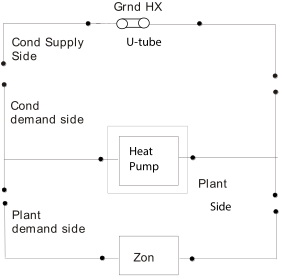
\includegraphics[width=0.9\textwidth, height=0.9\textheight, keepaspectratio=true]{media/image184.png}
\caption{Schematic of EnergyPlus Ground Loop Heat Exchanger \protect \label{fig:schematic-of-energyplus-ground-loop-heat-001}}
\end{figure}

First, the equation fit model objects are described. This model has two sets of coefficients, one for the heating mode and other for the cooling mode.

\subsection{HeatPump:WaterToWater:EquationFit:Cooling}\label{heatpumpwatertowaterequationfitcooling}

\subsubsection{Inputs}\label{inputs-12-012}

\paragraph{Field: Name}\label{field-name-11-010}

This alpha field contains the identifying name for the ground source heat pump.

\paragraph{Field: Source Side Inlet Node Name}\label{field-source-side-inlet-node-name}

This alpha field contains the heat pump's source side inlet node name.

\paragraph{Field: Source Side Outlet Node Name}\label{field-source-side-outlet-node-name}

This alpha field contains the heat pump's source side outlet node name.

\paragraph{Field: Load Side Inlet Node Name}\label{field-load-side-inlet-node-name}

This alpha field contains the heat pump's load side inlet node name.

\paragraph{Field: Load Side Outlet Node Name}\label{field-load-side-outlet-node-name}

This alpha field contains the heat pump's load side outlet node name.

\paragraph{Field: Rated Load Side Flow Rate}\label{field-rated-load-side-flow-rate}

This numeric field contains the rated volumetric flow rate on the load side of the heat pump in m3/s. This corresponds to the highest load side heat transfer rate listed in the catalog data.

\paragraph{Field: Rated Source Side Flow Rate}\label{field-rated-source-side-flow-rate}

This numeric field contains the rated volumetric flow rate on the source side of the heat pump in m3/s. This corresponds to the highest load side heat transfer rate listed in the catalog data.

\paragraph{Field: Rated Cooling Capacity}\label{field-rated-cooling-capacity}

This numeric field contains the rated cooling capacity of the heat pump in W. This corresponds to the highest load side heat transfer rate listed in the catalog data.

\paragraph{Field: Rated Cooling Power Consumption}\label{field-rated-cooling-power-consumption}

Rated cooling power consumption, in W.

\paragraph{Fields: Cooling Capacity Coefficients 1-5}\label{fields-cooling-capacity-coefficients-1-5}

Five fields are used to describe the coefficients for the Cooling Capacity curve. More details on how these coefficients are used are described in the Engineering Reference.

\paragraph{Field: Cooling Compressor Power Coefficients 1-5}\label{field-cooling-compressor-power-coefficients-1-5}

Five fields are used to decribe the coefficients for the Cooling Compressor Power curve.

An idf example:

\begin{lstlisting}

HeatPump:WaterToWater:EquationFit:Cooling,
  GshpCLG,                 !- Name
  GshpCLG SourceSide Inlet Node,      !- Source Side Inlet Node Name
  GshpCLG SourceSide Outlet Node,     !- Source Side Outlet Node Name
  GshpCLG LoadSide Inlet Node,        !- Load Side Inlet Node Name
  GshpCLG LoadSide Outlet Node,       !- Load Side Outlet Node Name
  1.89E-03,                !- Rated Load Side Flow Rate {m3/s}
  1.89E-03,                !- Rated Source Side Flow Rate {m3/s}
  39890.91,                !- Rated Cooling Capacity {W}
  4790.00,                 !- Rated Cooling Power Consumption {W}
  -1.52030596,             !- Cooling Capacity Coefficient 1
  3.46625667,              !- Cooling Capacity Coefficient 2
  -1.32267797,             !- Cooling Capacity Coefficient 3
  0.09395678,              !- Cooling Capacity Coefficient 4
  0.038975504,             !- Cooling Capacity Coefficient 5
  -8.59564386,             !- Cooling Compressor Power Coefficient 1
  0.96265085,              !- Cooling Compressor Power Coefficient 2
  8.69489229,              !- Cooling Compressor Power Coefficient 3
  0.02501669,              !- Cooling Compressor Power Coefficient 4
  -0.20132665;             !- Cooling Compressor Power Coefficient 5
\end{lstlisting}

\subsubsection{Outputs}\label{outputs-12-004}

This section describes the outputs available for the water to water heat pump, equation fit model; both cooling and heating.

\begin{itemize}
\item
  HVAC,Sum,Water to Water Heat Pump Electric Energy {[}J{]}
\item
  HVAC,Sum,Water to Water Heat Pump Load Side Heat Transfer Energy {[}J{]}
\item
  HVAC,Sum,Water to Water Heat Pump Source Side Heat Transfer Energy {[}J{]}
\item
  HVAC,Average,Water to Water Heat Pump Electric Power {[}W{]}
\item
  HVAC,Average,Water to Water Heat Pump Load Side Heat Transfer Rate {[}W{]}
\item
  HVAC,Average,Water to Water Heat Pump Source Side Heat Transfer Rate {[}W{]}
\item
  HVAC,Average,Water to Water Heat Pump Load Side Outlet Temperature {[}°C{]}
\item
  HVAC,Average,Water to Water Heat Pump Load Side Inlet Temperature {[}°C{]}
\item
  HVAC,Average,Water to Water Heat Pump Source Side Outlet Temperature {[}°C{]}
\item
  HVAC,Average,Water to Water Heat Pump Source Side Inlet Temperature {[}°C{]}
\item
  HVAC,Average,Water to Water Heat Pump Load Side Mass Flow Rate {[}kg/s{]}
\item
  HVAC,Average,Water to Water Heat Pump Source Side Mass Flow Rate {[}kg/s{]}
\end{itemize}

\paragraph{Water to Water Heat Pump Electric Energy {[}J{]}}\label{water-to-water-heat-pump-electric-energy-j}

This output variable represents the cumulative energy used by the compressor. The values are calculated for each HVAC system time step being simulated, and the results are summed across the reporting period.

\paragraph{Water to Water Heat Pump Load Side Heat Transfer Energy {[}J{]}}\label{water-to-water-heat-pump-load-side-heat-transfer-energy-j}

This output variable represents the cumulative heat transfer across the load side coil. The values are calculated for each HVAC system time step being simulated, and the results are summed across the reporting period.

\paragraph{Water to Water Heat Pump Source Side Heat Transfer Energy {[}J{]}}\label{water-to-water-heat-pump-source-side-heat-transfer-energy-j}

This output variable represents the cumulative heat transfer across the source side coil. The values are calculated for each HVAC system time step being simulated, and the results are summed across the reporting period.

\paragraph{Water to Water Heat Pump Electric Power {[}W{]}}\label{water-to-water-heat-pump-electric-power-w}

This output variable represents the compressor power required to run the heat pump. The values are calculated for each HVAC system time step being simulated, and the results are averaged for the time step being reported.

\paragraph{Water to Water Heat Pump Load Side Heat Transfer Rate {[}W{]}}\label{water-to-water-heat-pump-load-side-heat-transfer-rate-w}

This output variable represents the heat transfer across the load side coil. The values are calculated for each HVAC system time step being simulated, and the results are averaged for the time step being reported.

\paragraph{Water to Water Heat Pump Source Side Heat Transfer Rate {[}W{]}}\label{water-to-water-heat-pump-source-side-heat-transfer-rate-w}

This output variable represents the heat transfer across the source side coil. The values are calculated for each HVAC system time step being simulated, and the results are averaged for the time step being reported.

\paragraph{Water to Water Heat Pump Load Side Outlet Temperature {[}C{]}}\label{water-to-water-heat-pump-load-side-outlet-temperature-c}

This output variable represents the average fluid temperature leaving the load side coil. The values are calculated for each HVAC system time step being simulated, and the results are averaged for the time step being reported.

\paragraph{Water to Water Heat Pump Load Side Inlet Temperature {[}C{]}}\label{water-to-water-heat-pump-load-side-inlet-temperature-c}

This output variable represents the average fluid temperature entering the load side coil.~ The values are calculated for each HVAC system time step being simulated, and the results are averaged for the time step being reported.

\paragraph{Water to Water Heat Pump Source Side Outlet Temperature {[}C{]}}\label{water-to-water-heat-pump-source-side-outlet-temperature-c}

This output variable represents the average fluid temperature leaving the source side coil. The values are calculated for each HVAC system time step being simulated, and the results are averaged for the time step being reported.

\paragraph{Water to Water Heat Pump Source Side Inlet Temperature {[}C{]}}\label{water-to-water-heat-pump-source-side-inlet-temperature-c}

This output variable represents the average fluid temperature entering the source side coil.~ The values are calculated for each HVAC system time step being simulated, and the results are averaged for the time step being reported.

\paragraph{Water to Water Heat Pump Load Side Mass Flow Rate {[}kg/s{]}}\label{water-to-water-heat-pump-load-side-mass-flow-rate-kgs}

This output variable represents the average fluid flow rate through the load side coil. The values are calculated for each HVAC system time step being simulated, and the results are averaged for the time step being reported.

\paragraph{Water to Water Heat Pump Source Side Mass Flow Rate {[}kg/s{]}}\label{water-to-water-heat-pump-source-side-mass-flow-rate-kgs}

This output variable represents the average fluid flow rate through the source side coil. The values are calculated for each HVAC system time step being simulated, and the results are averaged for the time step being reported.

\subsection{HeatPump:WaterToWater:EquationFit:Heating}\label{heatpumpwatertowaterequationfitheating}

\subsubsection{Inputs}\label{inputs-13-010}

\paragraph{Field: Name}\label{field-name-12-008}

This alpha field contains the identifying name for the ground source heat pump.

\paragraph{Field: Source Side Inlet Node Name}\label{field-source-side-inlet-node-name-1}

This alpha field contains the heat pump's source side inlet node name.

\paragraph{Field: Source Side Outlet Node Name}\label{field-source-side-outlet-node-name-1}

This alpha field contains the heat pump's source side outlet node name.

\paragraph{Field: Load Side Inlet Node Name}\label{field-load-side-inlet-node-name-1}

This alpha field contains the heat pump's load side inlet node name.

\paragraph{Field: Load Side Outlet Node Name}\label{field-load-side-outlet-node-name-1}

This alpha field contains the heat pump's load side outlet node name.

\paragraph{Field: Rated Load Side Flow Rate}\label{field-rated-load-side-flow-rate-1}

This numeric field contains the rated volumetric flow rate on the load side of the heat pump in m3/s. This corresponds to the highest load side heat transfer rate listed in the catalog data.

\paragraph{Field: Rated Source Side Flow Rate}\label{field-rated-source-side-flow-rate-1}

This numeric field contains the rated volumetric flow rate on the source side of the heat pump in m3/s. This corresponds to the highest load side heat transfer rate listed in the catalog data.

\paragraph{Field: Rated Heating Capacity}\label{field-rated-heating-capacity-000}

This numeric field contains the rated heating capacity of the heat pump in W. This corresponds to the highest load side heat transfer rate listed in the catalog data.

\paragraph{Field: Rated Heating Power Consumption}\label{field-rated-heating-power-consumption}

Rated heating power consumption, in W.

\paragraph{Fields: Heating Capacity Coefficients 1-5}\label{fields-heating-capacity-coefficients-1-5}

Five fields are used to describe the coefficients for the Heating Capacity curve. More details on how these coefficients are used are described in the Engineering Reference.

\paragraph{Field: Heating Compressor Power Coefficients 1-5}\label{field-heating-compressor-power-coefficients-1-5}

Five fields are used to describe the coefficients for the Heating Compressor Power curve.

An idf example:

\begin{lstlisting}

HeatPump:WaterToWater:EquationFit:Heating,
  GshpHeating,             !- Name
  GshpHeating SourceSide Inlet Node,      !- Source Side Inlet Node Name
  GshpHeating SourceSide Outlet Node,     !- Source Side Outlet Node Name
  GshpHeating LoadSide Inlet Node,        !- Load Side Inlet Node Name
  GshpHeating LoadSide Outlet Node,       !- Load Side Outlet Node Name
  1.89E-03,                !- Rated Load Side Flow Rate {m3/s}
  1.89E-03,                !- Rated Source Side Flow Rate {m3/s}
  39040.92,                !- Rated Heating Capacity {W}
  5130.00,                 !- Rated Heating Power Consumption {W}
  -3.33491153,             !- Heating Capacity Coefficient 1
  -0.51451946,             !- Heating Capacity Coefficient 2
  4.51592706,              !- Heating Capacity Coefficient 3
  0.01797107,              !- Heating Capacity Coefficient 4
  0.155797661,             !- Heating Capacity Coefficient 5
  -8.93121751,             !- Heating Compressor Power Coefficient 1
  8.57035762,              !- Heating Compressor Power Coefficient 2
  1.29660976,              !- Heating Compressor Power Coefficient 3
  -0.21629222,             !- Heating Compressor Power Coefficient 4
  0.033862378;             !- Heating Compressor Power Coefficient 5
\end{lstlisting}

Next, the parameter estimation model objects are described. This model has two sets of parameters, one for the heating mode and other for the cooling mode.

\subsection{HeatPump:WaterToWater:ParameterEstimation:Cooling}\label{heatpumpwatertowaterparameterestimationcooling}

\subsubsection{Inputs}\label{inputs-14-010}

\paragraph{Field: Name}\label{field-name-13-007}

This alpha field contains the identifying name for the ground source heat pump.

\paragraph{Field: Source Side Inlet Node Name}\label{field-source-side-inlet-node-name-2}

This alpha field contains the heat pump's source side inlet node name.

\paragraph{Field: Source Side Outlet Node Name}\label{field-source-side-outlet-node-name-2}

This alpha field contains the heat pump's source side outlet node name.

\paragraph{Field: Load Side Inlet Node Name}\label{field-load-side-inlet-node-name-2}

This alpha field contains the heat pump's load side inlet node name.

\paragraph{Field: Load Side Outlet Node Name}\label{field-load-side-outlet-node-name-2}

This alpha field contains the heat pump's load side outlet node name.

\paragraph{Field: Nominal COP}\label{field-nominal-cop-4}

This numeric field contains the nominal coefficient of performance of the heat pump.

\paragraph{Field: Nominal Capacity}\label{field-nominal-capacity-8}

This numeric field contains the nominal capacity of the heat pump in Watts.

\paragraph{Field: Minimum Part Load Ratio}\label{field-minimum-part-load-ratio-11}

This numeric field contains the minimum part load ratio of the heat pump usually set to 0.

\paragraph{Field: Maximum Part Load Ratio}\label{field-maximum-part-load-ratio-11}

This numeric field contains the maximum part load ratio of the heat pump usually set to 1.

\paragraph{Field: Optimum Part Load Ratio}\label{field-optimum-part-load-ratio-11}

This numeric field contains the optimal part load ratio of the heat pump usually set to 1.

\paragraph{Field: Load Side Flow Rate}\label{field-load-side-flow-rate}

This numeric field contains the volumetric flow rate on the load side of the heat pump in m3/s

\paragraph{Field: Source Side Flow Rate}\label{field-source-side-flow-rate}

This numeric field contains the volumetric flow rate on the source side of the heat pump in m3/s

\paragraph{Field: Load Side Heat Transfer Coefficient}\label{field-load-side-heat-transfer-coefficient}

This numeric field contains Estimated parameter load side heat transfer coefficient W/K.

\paragraph{Field: Source Side Heat Transfer Coefficient}\label{field-source-side-heat-transfer-coefficient-000}

This numeric field contains Estimated parameter source side heat transfer coefficient W/K.

\paragraph{Field: Piston Displacement}\label{field-piston-displacement}

This numeric field contains the Estimated parameter displacement of the reciprocating compressor in m3/s.

\paragraph{Field: Compressor Clearance Factor}\label{field-compressor-clearance-factor-000}

This numeric field contains the Estimated parameter clearance factor of the reciprocating compressor.

\paragraph{Field: Compressor Suction and Discharge Pressure Drop}\label{field-compressor-suction-and-discharge-pressure-drop}

This numeric field contains the estimated parameter the pressure drop at compressor suction and discharge in Pascals (N/m2).

\paragraph{Field: Superheating}\label{field-superheating}

This numeric field contains the estimated parameter superheat at the evaporator outlet in °C.

\paragraph{Field: Constant Part of Electromechanical Power Losses}\label{field-constant-part-of-electromechanical-power-losses}

This numeric field contains the estimated parameter power loss, which accounts for the loss of work due mechanical and electrical losses in the compressor in Watts.

\paragraph{Field: Loss Factor}\label{field-loss-factor}

This numeric field contains the factor of electromechanical loss that is proportional to the theoretical power percentage.

\paragraph{Field: High Pressure Cut Off}\label{field-high-pressure-cut-off}

This numeric field contains the design pressure limit of the compressor in Pascals (N/m2).

\paragraph{Field: Low Pressure Cut Off}\label{field-low-pressure-cut-off}

This numeric field contains the design low-pressure limit of the compressor in Pascals (N/m2).

An idf example:

\begin{lstlisting}

HeatPump:WaterToWater:ParameterEstimation:Cooling,
      GshpCLG,                 !- Water to Water Heat Pump Name
      GshpCLG SourceSide Inlet Node,  !- Source Side Inlet Node
      GshpCLG SourceSide Outlet Node,  !- Source Side Outlet Node
      GshpCLG LoadSide Inlet Node,  !- Load Side Inlet Node
      GshpCLG LoadSide Outlet Node,  !- Load Side Outlet Node
      3.5,                     !- Nominal COP
      45000,                   !- Nominal Capacity {W}
      0.0,                     !- Min PLR
      1,                       !- Max PLR
      1,                       !- optimum PLR
      .003,                    !- Load side Flow Rate {m3/s}
      .003,                    !- Source Side Flow Rate {m3/s}
      7761,                    !- Load side Heat Transfer Coefficient {W/K}
      3998,                    !- Source Side Heat Transfer Coefficient {W/K}
      .012544,                 !- Piston Displacement {m3/s}
      .05469,                  !- Compressor Clearance Factor %
      92156.2,                 !- Compressor Suction And Discharge Pressure Drop {Pa}
      4.8907,                  !- Superheating {C}
      2803.9,                  !- Constant Part of Electro Mechanical Power Losses {W}
      .699,                    !- Loss Factor
      0.0,                     !- High Pressure Cut off {Pa}
      0.0;                     !- LowPressure Cut off {Pa}
\end{lstlisting}

\subsection{HeatPump:WaterToWater:ParameterEstimation:Heating}\label{heatpumpwatertowaterparameterestimationheating}

\subsubsection{Inputs}\label{inputs-15-010}

\paragraph{Field: Name}\label{field-name-14-006}

This alpha field contains the identifying name for the ground source heat pump.

\paragraph{Field: Source Side Inlet Node Name}\label{field-source-side-inlet-node-name-3}

This alpha field contains the heat pump's source side inlet node name.

\paragraph{Field: Source Side Outlet Node Name}\label{field-source-side-outlet-node-name-3}

This alpha field contains the heat pump's source side outlet node name.

\paragraph{Field: Load Side Inlet Node Name}\label{field-load-side-inlet-node-name-3}

This alpha field contains the heat pump's load side inlet node name.

\paragraph{Field: Load Side Outlet Node Name}\label{field-load-side-outlet-node-name-3}

This alpha field contains the heat pump's load side outlet node name.

\paragraph{Field: Nominal COP}\label{field-nominal-cop-5}

This numeric field contains the nominal coefficient of performance of the heat pump.

\paragraph{Field: Nominal Capacity}\label{field-nominal-capacity-9}

This numeric field contains the nominal capacity of the heat pump in Watts.

\paragraph{Field: Minimum Part Load Ratio}\label{field-minimum-part-load-ratio-12}

This numeric field contains the minimum part load ratio of the heat pump usually set to 0.

\paragraph{Field: Maximum Part Load Ratio}\label{field-maximum-part-load-ratio-12}

This numeric field contains the maximum part load ratio of the heat pump usually set to 1.

\paragraph{Field: Optimum Part Load Ratio}\label{field-optimum-part-load-ratio-12}

This numeric field contains the optimal part load ratio of the heat pump usually set to 1.

\paragraph{Field: Load Side Flow Rate}\label{field-load-side-flow-rate-1}

This numeric field contains the volumetric flow rate on the load side of the heat pump in m3/s

\paragraph{Field: Source Side Flow Rate}\label{field-source-side-flow-rate-1}

This numeric field contains the volumetric flow rate on the source side of the heat pump in m3/s

\paragraph{Field: Load Side Heat Transfer Coefficient}\label{field-load-side-heat-transfer-coefficient-1}

This numeric field contains Estimated parameter load side heat transfer coefficient W/K.

\paragraph{Field: Source Side Heat Transfer Coefficient}\label{field-source-side-heat-transfer-coefficient-1-000}

This numeric field contains Estimated parameter source side heat transfer coefficient W/K.

\paragraph{Field: Piston Displacement}\label{field-piston-displacement-1}

This numeric field contains the Estimated parameter displacement of the reciprocating compressor in m3/s.

\paragraph{Field: Compressor Clearance Factor}\label{field-compressor-clearance-factor-1-000}

This numeric field contains the Estimated parameter clearance factor of the reciprocating compressor.

\paragraph{Field: Compressor Suction and Discharge Pressure Drop}\label{field-compressor-suction-and-discharge-pressure-drop-1}

This numeric field contains the estimated parameter the pressure drop at compressor suction and discharge in Pascals (N/m2).

\paragraph{Field: Superheating}\label{field-superheating-1}

This numeric field contains the estimated parameter superheat at the evaporator outlet in °C.

\paragraph{Field: Constant Part of Electromechanical Power Losses}\label{field-constant-part-of-electromechanical-power-losses-1}

This numeric field contains the estimated parameter power loss, which accounts for the loss of work due mechanical and electrical losses in the compressor in Watts.

\paragraph{Field: Loss Factor}\label{field-loss-factor-1}

This numeric field contains the factor of electromechanical loss that is proportional to the theoretical power percentage.

\paragraph{Field: High Pressure Cut Off}\label{field-high-pressure-cut-off-1}

This numeric field contains the design pressure limit of the compressor in Pascals (N/m2).

\paragraph{Field: Low Pressure Cut Off}\label{field-low-pressure-cut-off-1}

This numeric field contains the design low-pressure limit of the compressor in Pascals (N/m2).

An idf example:

\begin{lstlisting}

HeatPump:WaterToWater:ParameterEstimation:Heating,
      GshpHeating,             !- Water to Water Heat Pump Name
      GshpHeating SourceSide Inlet Node,  !- Source Side Inlet Node
      GshpHeating SourceSide Outlet Node,  !- Source Side Outlet Node
      GshpHeating LoadSide Inlet Node,  !- Load Side Inlet Node
      GshpHeating LoadSide Outlet Node,  !- Load Side Outlet Node
      3.5,                     !- Nominal COP
      50000,                   !- Nominal Capacity {W}
      0.0,                     !- Min PLR
      1,                       !- Max PLR
      1,                       !- optimum PLR
      .003,                    !- Load side Flow Rate {m3/s}
      .003,                    !- Source Side Flow Rate {m3/s}
      7761,                    !- Load side Heat Transfer Coefficient {W/K}
      3998,                    !- Source Side Heat Transfer Coefficient {W/K}
      .012544,                 !- Piston Displacement {m3/s}
      .05469,                  !- Compressor Clearance Factor %
      92156.2,                 !- Compressor Suction And Dischrage Pressure Drop {Pa}
      4.8907,                  !- Superheating {C}
      2803.9,                  !- Constant Part Of Electro Mechanical Power Losses {W}
      .699,                    !- Loss Factor
      0.0,                     !- High Pressure Cut off {Pa}
      0.0;                     !- LowPressure Cut off {Pa}
\end{lstlisting}

Since the heat pump is defined with two separate objects (one for heating, one for cooling), the connections to the condenser has to be done carefully. The example below shows the configuration for parameter estimation objects. The same specifications and configuration also applies to the equation fit model.

\paragraph{Steps to specify the Ground Source Heat Pump}\label{steps-to-specify-the-ground-source-heat-pump}

For the heating mode:

\begin{enumerate}
\def\labelenumi{\arabic{enumi}.}
\item
  Specify a branch for the Heat pump in hot water loop .
\item
  Include the branch name in the splitter and mixer branches.
\item
  Add a branch in condenser loop and include its name in the respective splitter and mixer.
\end{enumerate}

\textbf{! in hot water loop}

\begin{lstlisting}

BRANCH, Heating GshpHeating Branch,
    ,
    ,
    HeatPump:WatertoWater:ParameterEstimatinon:Heating,
    GshpHeating,
    GshpHeating LoadSide Inlet Node,
    GshpHeating LoadSide Outlet Node,
    ACTIVE;
\end{lstlisting}

\textbf{!in condenser loop}

\begin{lstlisting}

BRANCH, GshpHeating SourceSide Branch,
    ,
    ,
    HeatPump:WatertoWater:ParameterEstimatinon:Heating,
    GshpHeating,
    GshpHeating SourceSide Inlet Node,
    GshpHeating SourceSide Outlet Node,
    ACTIVE;
\end{lstlisting}

Example of Heat Pump Links

For the cooling mode:

1.~Specify a branch for the Heat pump in chilled water loop .

\begin{enumerate}
\def\labelenumi{\arabic{enumi}.}
\setcounter{enumi}{1}
\tightlist
\item
  Include the branch name in the splitter and mixer branches.
\end{enumerate}

3.~Add a branch in condenser loop and include its name in the respective splitter and mixer.

\textbf{! in chilled water loop}

\begin{lstlisting}

BRANCH,GshpCLG1 Chiller Branch,
    ,
    ,
    HeatPump:WatertoWater:ParameterEstimatinon:Cooling, GshpCLG1,
    GshpCLG LoadSide Inlet Node1,
    GshpCLG LoadSide Outlet Node1,
    Active;
\end{lstlisting}

\textbf{!in condenser loop}

\begin{lstlisting}

BRANCH, GshpCLG1 Condenser Branch,
    ,
    ,
    HeatPump:WatertoWater:ParameterEstimatinon:Cooling, GshpCLG1,
    GshpCLG SourceSide Inlet Node1,
    GshpCLG SourceSide Outlet Node1,
    ACTIVE;
\end{lstlisting}

\subsubsection{Outputs}\label{outputs-13-003}

This section describes the outputs available for the water to water heat pump, parameter estimation model; both cooling and heating.

\begin{itemize}
\item
  HVAC,Average,Water to Water Heat Pump Electric Power {[}W{]}
\item
  HVAC,Average,Water to Water Heat Pump Electric Power {[}W{]}
\item
  HVAC,Sum,Water to Water Heat Pump Electric Energy {[}J{]}
\item
  HVAC,Sum,Water to Water Heat Pump Electric Energy {[}J{]}
\item
  HVAC,Average,Water to Water Heat Pump Load Side Heat Transfer Rate {[}W{]}
\item
  HVAC,Average,Water to Water Heat Pump Load Side Heat Transfer Rate {[}W{]}
\item
  HVAC,Sum,Water to Water Heat Pump Load Side Heat Transfer Energy {[}J{]}
\item
  HVAC,Sum,Water to Water Heat Pump Load Side Heat Transfer Energy {[}J{]}
\item
  HVAC,Average,Water to Water Heat Pump Source Side Heat Transfer Rate {[}W{]}
\item
  HVAC,Average,Water to Water Heat Pump Source Side Heat Transfer Rate {[}W{]}
\item
  HVAC,Sum,Water to Water Heat Pump Source Side Heat Transfer Energy {[}J{]}
\item
  HVAC,Sum,Water to Water Heat Pump Source Side Heat Transfer Energy {[}J{]}
\item
  HVAC,Average,Water to Water Heat Pump Load Side Outlet Temperature {[}°C{]}
\item
  HVAC,Average,Water to Water Heat Pump Load Side Outlet Temperature {[}°C{]}
\item
  HVAC,Average,Water to Water Heat Pump Load Side Inlet Temperature {[}°C{]}
\item
  HVAC,Average,Water to Water Heat Pump Load Side Inlet Temperature {[}°C{]}
\item
  HVAC,Average,Water to Water Heat Pump Source Side Outlet Temperature {[}°C{]}
\item
  HVAC,Average,Water to Water Heat Pump Source Side Outlet Temperature {[}°C{]}
\item
  HVAC,Average,Water to Water Heat Pump Source Side Inlet Temperature {[}°C{]}
\item
  HVAC,Average,Water to Water Heat Pump Source Side Inlet Temperature {[}°C{]}
\item
  HVAC,Average,Water to Water Heat Pump Load Side Mass Flow Rate {[}kg/s{]}
\item
  HVAC,Average,Water to Water Heat Pump Load Side Mass Flow Rate {[}kg/s{]}
\item
  HVAC,Average,Water to Water Heat Pump Source Side Mass Flow Rate {[}kg/s{]}
\item
  HVAC,Average,Water to Water Heat Pump Source Side Mass Flow Rate {[}kg/s{]}
\end{itemize}

\paragraph{Water to Water Heat Pump Electric Power {[}W{]}}\label{water-to-water-heat-pump-electric-power-w-1}

\paragraph{Water to Water Heat Pump Electric Power {[}W{]}}\label{water-to-water-heat-pump-electric-power-w-2}

This output variable represents the compressor power required to run the heat pump. The values are calculated for each HVAC system time step being simulated, and the results are averaged for the time step being reported.

\paragraph{Water to Water Heat Pump Electric Energy {[}J{]}}\label{water-to-water-heat-pump-electric-energy-j-1}

\paragraph{Water to Water Heat Pump Electric Energy {[}J{]}}\label{water-to-water-heat-pump-electric-energy-j-2}

This output variable represents the cumulative energy used by the compressor. The values are calculated for each HVAC system time step being simulated, and the results are summed across the reporting period.

\paragraph{Water to Water Heat Pump Load Side Heat Transfer Rate {[}W{]}}\label{water-to-water-heat-pump-load-side-heat-transfer-rate-w-1}

\paragraph{Water to Water Heat Pump Load Side Heat Transfer Rate {[}W{]}}\label{water-to-water-heat-pump-load-side-heat-transfer-rate-w-2}

This output variable represents the heat transfer across the load side coil. The values are calculated for each HVAC system time step being simulated, and the results are averaged for the time step being reported.

\paragraph{Water to Water Heat Pump Load Side Heat Transfer Energy {[}J{]}}\label{water-to-water-heat-pump-load-side-heat-transfer-energy-j-1}

\paragraph{Water to Water Heat Pump Load Side Heat Transfer Energy {[}J{]}}\label{water-to-water-heat-pump-load-side-heat-transfer-energy-j-2}

This output variable represents the cumulative heat transfer across the load side coil. The values are calculated for each HVAC system time step being simulated, and the results are summed across the reporting period.

\paragraph{Water to Water Heat Pump Source Side Heat Transfer Rate {[}W{]}}\label{water-to-water-heat-pump-source-side-heat-transfer-rate-w-1}

\paragraph{Water to Water Heat Pump Source Side Heat Transfer Rate {[}W{]}}\label{water-to-water-heat-pump-source-side-heat-transfer-rate-w-2}

This output variable represents the heat transfer across the source side coil. The values are calculated for each HVAC system time step being simulated, and the results are averaged for the time step being reported.

\paragraph{Water to Water Heat Pump Source Side Heat Transfer Energy {[}J{]}}\label{water-to-water-heat-pump-source-side-heat-transfer-energy-j-1}

\paragraph{Water to Water Heat Pump Source Side Heat Transfer Energy {[}J{]}}\label{water-to-water-heat-pump-source-side-heat-transfer-energy-j-2}

This output variable represents the cumulative heat transfer across the source side coil. The values are calculated for each HVAC system time step being simulated, and the results are summed across the reporting period.

\paragraph{Water to Water Heat Pump Load Side Outlet Temperature {[}C{]}}\label{water-to-water-heat-pump-load-side-outlet-temperature-c-1}

\paragraph{Water to Water Heat Pump Load Side Outlet Temperature {[}C{]}}\label{water-to-water-heat-pump-load-side-outlet-temperature-c-2}

This output variable represents the average fluid temperature leaving the load side coil. The values are calculated for each HVAC system time step being simulated, and the results are averaged for the time step being reported.

\paragraph{Water to Water Heat Pump Load Side Inlet Temperature {[}C{]}}\label{water-to-water-heat-pump-load-side-inlet-temperature-c-1}

\paragraph{Water to Water Heat Pump Load Side Inlet Temperature {[}C{]}}\label{water-to-water-heat-pump-load-side-inlet-temperature-c-2}

This output variable represents the average fluid temperature entering the load side coil.~ The values are calculated for each HVAC system time step being simulated, and the results are averaged for the time step being reported.

\paragraph{Water to Water Heat Pump Source Side Outlet Temperature {[}C{]}}\label{water-to-water-heat-pump-source-side-outlet-temperature-c-1}

\paragraph{Water to Water Heat Pump Source Side Outlet Temperature °C{]}}\label{water-to-water-heat-pump-source-side-outlet-temperature-c-2}

This output variable represents the average fluid temperature leaving the source side coil. The values are calculated for each HVAC system time step being simulated, and the results are averaged for the time step being reported.

\paragraph{Water to Water Heat Pump Source Side Inlet Temperature {[}C{]}}\label{water-to-water-heat-pump-source-side-inlet-temperature-c-1}

\paragraph{Water to Water Heat Pump Source Side Inlet Temperature {[}C{]}}\label{water-to-water-heat-pump-source-side-inlet-temperature-c-2}

This output variable represents the average fluid temperature entering the source side coil.~ The values are calculated for each HVAC system time step being simulated, and the results are averaged for the time step being reported.

\paragraph{Water to Water Heat Pump Load Side Mass Flow Rate {[}kg/s{]}}\label{water-to-water-heat-pump-load-side-mass-flow-rate-kgs-1}

\paragraph{Water to Water Heat Pump Load Side Mass Flow Rate {[}kg/s{]}}\label{water-to-water-heat-pump-load-side-mass-flow-rate-kgs-2}

This output variable represents the average fluid flow rate through the load side coil. The values are calculated for each HVAC system time step being simulated, and the results are averaged for the time step being reported.

\paragraph{Water to Water Heat Pump Source Side Mass Flow Rate {[}kg/s{]}}\label{water-to-water-heat-pump-source-side-mass-flow-rate-kgs-1}

\paragraph{Water to Water Heat Pump Source Side Mass Flow Rate {[}kg/s{]}}\label{water-to-water-heat-pump-source-side-mass-flow-rate-kgs-2}

This output variable represents the average fluid flow rate through the source side coil. The values are calculated for each HVAC system time step being simulated, and the results are averaged for the time step being reported.

\subsection{DistrictCooling}\label{districtcooling}

When the user is not interested in a plant simulation or there is some centralized source of chilled water, the following object can be used in the input.

\subsubsection{Inputs}\label{inputs-16-008}

\paragraph{Field: Name}\label{field-name-15-006}

This alpha field contains the identifying name for the district cooling (i.e., purchased chilled water).

\paragraph{Field: Chilled Water Inlet Node Name}\label{field-chilled-water-inlet-node-name-9}

This alpha field contains the identifying name for the district cooling inlet node.

\paragraph{Field: Chilled Water Outlet Node Name}\label{field-chilled-water-outlet-node-name-10}

This alpha field contains the identifying name for the district cooling outlet node.

\paragraph{Field: Nominal Capacity}\label{field-nominal-capacity-10}

This numeric field contains the nominal demand (W) that the district cooling will meet. This field is autosizable.

\paragraph{Field: Capacity Fraction Schedule Name}\label{field-capacity-fraction-schedule-name}

This alpha field contains the name of a schedule that describes how the nominal capacity varies over time.~ Values must non-negative. The capacity at a given point in time is determined by the product of the previous field and the value in this schedule. If the field is omitted or left blank, then the program assumes a schedule value of 1.0 all the time.

An example of this statement in an IDF is:

\begin{lstlisting}

DistrictCooling, Purchased Cooling,
          NODE_35,NODE_49,
          68000;
\end{lstlisting}

\subsubsection{Outputs}\label{outputs-14-003}

\begin{itemize}
\item
  HVAC,Average, District Cooling Chilled Water Rate {[}W{]}
\item
  HVAC,Sum, District Cooling Chilled Water Energy {[}J{]}
\item
  Zone,Meter, DistrictCooling:Plant {[}J{]}
\item
  Zone,Meter,Cooling: DistrictCooling {[}J{]}
\item
  HVAC,Average,District Cooling Rate {[}W{]}
\item
  HVAC,Average,District Cooling Inlet Temperature {[}C{]}
\item
  HVAC,Average,District Cooling Outlet Temperature {[}C{]}
\item
  HVAC,Average,District Cooling Mass Flow Rate {[}kg/s{]}
\end{itemize}

\paragraph{District Cooling Chilled Water Rate {[}W{]}}\label{district-cooling-chilled-water-rate-w}

\paragraph{District Cooling Chilled Water Energy {[}J{]}}\label{district-cooling-chilled-water-energy-j}

These outputs are the energy taken from purchased chilled water. Consumption is metered on Cooling:DistrictCooling, DistrictCooling:Plant, and DistrictCooling:Facility.

\paragraph{District Cooling Rate {[}W{]}}\label{district-cooling-rate-w}

This is the useful rate of cooling energy from purchased chilled water. For the current algorithm, this is the same as District Cooling Chilled Water Rate.

\paragraph{District Cooling Inlet Temperature {[}C{]}}\label{district-cooling-inlet-temperature-c}

\paragraph{District Cooling Outlet Temperature {[}C{]}}\label{district-cooling-outlet-temperature-c}

\paragraph{District Cooling Mass Flow Rate {[}kg/s{]}}\label{district-cooling-mass-flow-rate-kgs}

These outputs are the supply-side plant loop chilled water inlet and outlet temperatures and mass flow rate.

\subsection{DistrictHeating}\label{districtheating}

When the user is not interested in a plant simulation or there is some centralized source of hot water (district heating), the following object can be used in the input.

\subsubsection{Inputs}\label{inputs-17-006}

\paragraph{Field: Name}\label{field-name-16-006}

This alpha field contains the identifying name for the district heating (i.e., purchased hot water).

\paragraph{Field: Hot Water Inlet Node Name}\label{field-hot-water-inlet-node-name-2}

This alpha field contains the identifying name for the district heating inlet node.

\paragraph{Field: Hot Water Outlet Node Name}\label{field-hot-water-outlet-node-name-2}

This alpha field contains the identifying name for the district heating outlet node.

\paragraph{Field: Nominal Capacity}\label{field-nominal-capacity-11}

This numeric field contains the nominal demand (W) that the district heating will meet. This field is autosizable.

\paragraph{Field: Capacity Fraction Schedule Name}\label{field-capacity-fraction-schedule-name-1}

This alpha field contains the name of a schedule that describes how the nominal capacity varies over time.~ Values must non-negative. The capacity at a given point in time is determined by the product of the previous field and the value in this schedule. If the field is omitted or left blank, then the program assumes a schedule value of 1.0 all the time.

An example of this statement in an IDF is:

\begin{lstlisting}

DistrictHeating,Purchased Heating,
          NODE_30,NODE_29,
          1000000;
\end{lstlisting}

\subsubsection{Outputs}\label{outputs-15-002}

\begin{itemize}
\item
  HVAC,Average,District Heating Hot Water Rate {[}W{]}
\item
  HVAC,Sum,District Heating Hot Water Energy {[}J{]}
\item
  Zone,Meter,DistrictHeating:Plant {[}J{]}
\item
  Zone,Meter,Heating:DistrictHeating {[}J{]}
\item
  HVAC,Average,District Heating Rate {[}W{]}
\item
  HVAC,Average,District Heating Inlet Temperature {[}C{]}
\item
  HVAC,Average,District Heating Outlet Temperature {[}C{]}
\item
  HVAC,Average,District Heating Mass Flow Rate {[}kg/s{]}
\end{itemize}

\paragraph{District Heating Hot Water Rate {[}W{]}}\label{district-heating-hot-water-rate-w}

\paragraph{District Heating Hot Water Energy {[}J{]}}\label{district-heating-hot-water-energy-j}

These outputs are the energy taken from purchased hot water. Consumption is metered on Heating:DistrictHeating, DistrictHeating:Plant, and DistrictHeating:Facility.

\paragraph{District Heating Rate {[}W{]}}\label{district-heating-rate-w}

This is the useful rate of heating energy from purchased hot water. For the current algorithm, this is the same as District Heating Hot Water Rate.

\paragraph{District Heating Inlet Temperature {[}C{]}}\label{district-heating-inlet-temperature-c}

\paragraph{District Heating Outlet Temperature {[}C{]}}\label{district-heating-outlet-temperature-c}

\paragraph{District Heating Mass Flow Rate {[}kg/s{]}}\label{district-heating-mass-flow-rate-kgs}

These outputs are the supply-side plant loop hot water inlet and outlet temperatures and mass flow rate.

\subsection{PlantComponent:TemperatureSource}\label{plantcomponenttemperaturesource}

This object allows the simulation of a water (or other fluid) source at a user-specified temperature.~ This could include a river, well, or seawater source, or any other configuration where the fluid temperature being supplied by the component to the plant is known.~ The temperature may be a constant or scheduled.~ Of course, the scheduled value may also be overwritten via EMS in cases where the specified temperature should be calculated at run-time.

\subsubsection{Inputs}\label{inputs-18-006}

\paragraph{Field: Name}\label{field-name-17-005}

This field is the string identifier for this component.

\paragraph{Field: Inlet Node}\label{field-inlet-node-000}

This is the name of this component's inlet node for the plant connection.

\paragraph{Field: Outlet Node}\label{field-outlet-node-000}

This is the name of this component's outlet node for the plant connection. The source temperature is applied to this node when the component is active.

\paragraph{Field: Design Volume Flow Rate}\label{field-design-volume-flow-rate}

This numeric field contains the design value for component volume flow rate in m\(^{3}\)/s.~ This field may be autosized.

\paragraph{Field: Temperature Specification Type}\label{field-temperature-specification-type}

This string field specifies the behavior of the source temperature.~ Two inputs are allowed: Constant or Scheduled.~ For a constant condition, a single input value (the next field) is used as the returning temperature (component outlet temperature) throughout the entire simulation.~ For a scheduled condition, the name of a schedule (the following field) is used to allow the temperature to vary throughout the simulation.~ This schedule value may be actuated via EMS to allow further flexibility on temperature specification at run-time.

\paragraph{Field: Source Temperature}\label{field-source-temperature}

If the Temperature Specification Type field is Constant, then the value in this field is used as the source temperature (in C) throughout the entire simulation.

\paragraph{Field: Source Temperature Schedule Name}\label{field-source-temperature-schedule-name}

If the Temperature Specification Type field is Scheduled, then this is the name of a schedule entered in the IDF which specifies the dynamic temperature of this source object. The units of this schedule should be C.

And, as shown in an IDF:

\begin{lstlisting}

PlantComponent:TemperatureSource,
      FluidSource,             !- Name
      FluidSource Inlet Node,  !- Inlet Node
      FluidSource Outlet Node, !- Outlet Node
      Autosize,                !- Design Volume Flow Rate {m3/s}
      Constant,                !- Temperature Specification Type
      62,                      !- Source Temperature {C}
      ;                        !- Source Temperature Schedule Name
\end{lstlisting}

\subsubsection{Outputs}\label{outputs-16-000}

The following output variables are available for the temperature source plant components:

\begin{itemize}
\item
  HVAC,Average,Plant Temperature Source Component Mass Flow Rate {[}kg/s{]}
\item
  HVAC,Average,Plant Temperature Source Component Inlet Temperature {[}C{]}
\item
  HVAC,Average,Plant Temperature Source Component Outlet Temperature {[}C{]}
\item
  HVAC,Average,Plant Temperature Source Component Source Temperature {[}C{]}
\item
  HVAC,Average,Plant Temperature Source Component Heat Transfer Rate {[}W{]}
\item
  HVAC,Sum,Plant Temperature Source Component Heat Transfer Energy {[}J{]}
\end{itemize}

\paragraph{Plant Temperature Source Component Mass Flow Rate {[}kg/s{]}}\label{plant-temperature-source-component-mass-flow-rate-kgs}

The current mass flow rate of this component.

\paragraph{Plant Temperature Source Component Inlet Temperature {[}C{]}}\label{plant-temperature-source-component-inlet-temperature-c}

The current entering fluid temperature of this component.

\paragraph{Plant Temperature Source Component Outlet Temperature {[}C{]}}\label{plant-temperature-source-component-outlet-temperature-c}

The current outlet temperature of this component.

\paragraph{Plant Temperature Source Component Source Temperature {[}C{]}}\label{plant-temperature-source-component-source-temperature-c}

The current source temperature of this component.

\paragraph{Plant Temperature Source Component Heat Transfer Rate {[}W{]}}\label{plant-temperature-source-component-heat-transfer-rate-w}

The current heat transfer rate of this component, positive for outlet temperature \textgreater{} inlet temperature, or adding heat to the loop, or absorbing heat from the source.

\paragraph{Plant Temperature Source Component Heat Transfer Energy {[}J{]}}\label{plant-temperature-source-component-heat-transfer-energy-j}

The current heat transfer energy over the given reporting period of this component.

\subsection{CentralHeatPumpSystem}\label{centralheatpumpsystem}

This is a central geothermal application that contains one or more chiller-heaters centrally located in the building; the available chilled and/or hot water is then piped to the individual zones. Chiller-heaters used for this particular system can be of two types: 1) standard vapor-compression, non-reversible cycle chillers designed for heat recovery or 2) reversible-cycle, water-to-water heat pump chillers. Unlike a distributed ground source heat pump configuration where individual heat pumps are located in each zone, a centralized geothermal configuration has one or more chiller-heaters. Its function is to encapsulate the extra controls needed to turn individual chiller-heater modules on/off and whether they are to operate in cooling-only, heating-only or simultaneous cooling-heating mode and whether to connect the source water to the evaporator or condenser side. A variety of control schemes can be designed by setting schedules for both zone control types and individual chiller-heaters schedules.

The fluid used in this central system is usually water, and there is no sharing of condenser or evaporator water between multiple machines. However, the control logic is such that the source water can be delivered to individual chiller-heaters depending on their operating mode, e.g., modules in simultaneous cooling-heating mode receive no source water, modules in heating-only mode can have source water directed to their evaporator, or modules in cooling-only mode can have source water directed to their condenser; the decision on which module(s) receives the source water dictated by the `smart' controls. The following figures illustrate node interconnections between this central geothermal application and plant and condenser loops in various situations.

The order of the multiple chiller-heaters' operation is assumed to be sequential. In other words, the very first chiller-heater will be called at first to see if it meets all loads that the central heat pump system should meet. If the chiller-heater meets all loads, the rest chiller-heaters are assumed to be turned off. If not, the following chiller-heater will be called to meet the remaining loads until all loads are met in the order as defined in the set of individual chiller-heater objects below. The order of individual chiller-heater modules needs to be carefully arranged in case users are intended to see the performance of various combinations of different sizes of chiller-heaters in a central heat pump system.

\begin{figure}[hbtp] % fig 76
\centering
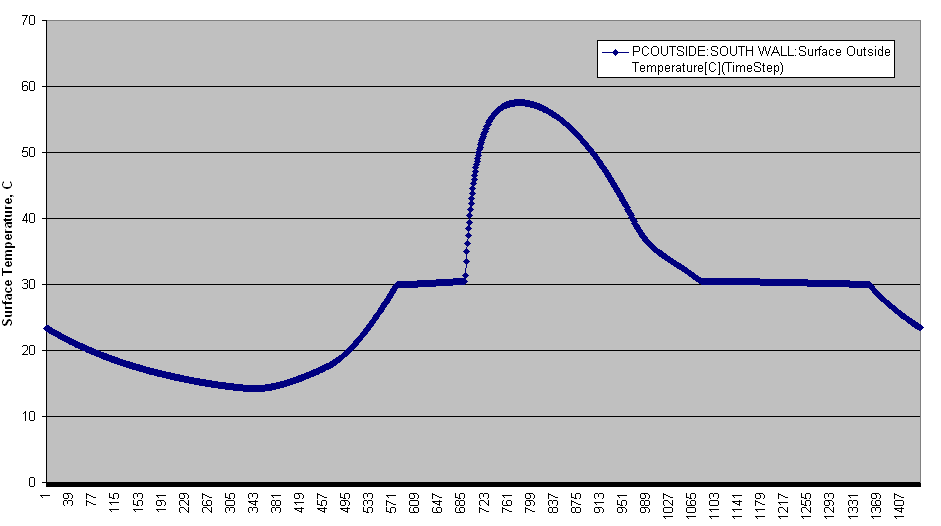
\includegraphics[width=0.9\textwidth, height=0.9\textheight, keepaspectratio=true]{media/image185.png}
\caption{Diagram of a central heat pump system with three chiller-heaters in cooling-only mode (Condensers reject heat to the ground source loop) \protect \label{fig:diagram-of-a-central-heat-pump-system-with}}
\end{figure}

\begin{figure}[hbtp] % fig 77
\centering
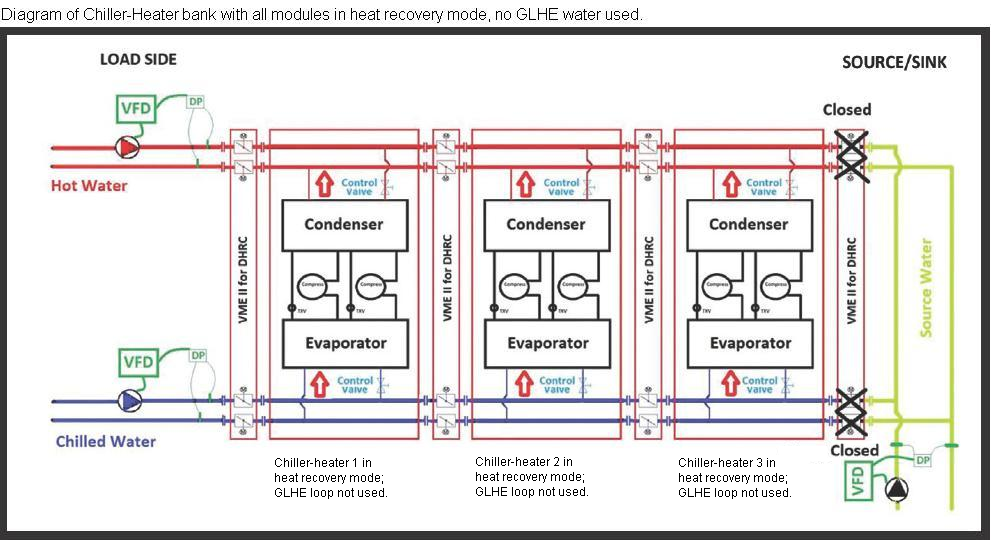
\includegraphics[width=0.9\textwidth, height=0.9\textheight, keepaspectratio=true]{media/image186.png}
\caption{Diagram of a central heat pump system with three chiller-heaters in heat recovery mode         (No heat is exchanged with the ground source loop) \protect \label{fig:diagram-of-a-central-heat-pump-system-with-001}}
\end{figure}

\begin{figure}[hbtp] % fig 78
\centering
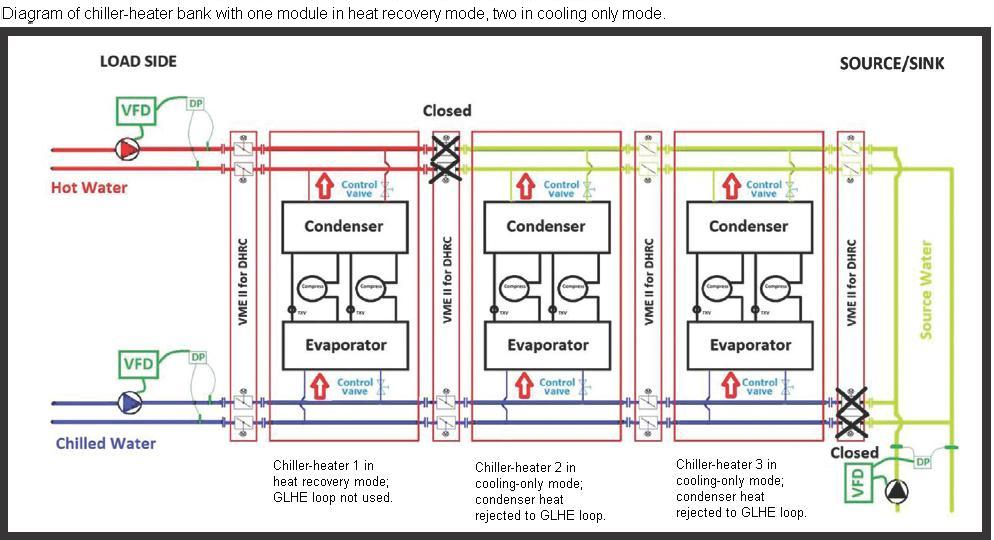
\includegraphics[width=0.9\textwidth, height=0.9\textheight, keepaspectratio=true]{media/image187.png}
\caption{Diagram of a central heat pump system with one chiller-heater in heat recovery mode and two chiller-heaters in cooling-only mode \protect \label{fig:diagram-of-a-central-heat-pump-system-with-002}}
\end{figure}

In the above example, the cooling load needs 3 chiller-heaters and the heating load needs 1 chiller heater. Chiller 1 is in heat recovery mode and isolated from the ground source loop while chillers 2 and 3 are in cooling-only mode, their condensers rejecting heat to the ground source loop.

\begin{figure}[hbtp] % fig 79
\centering
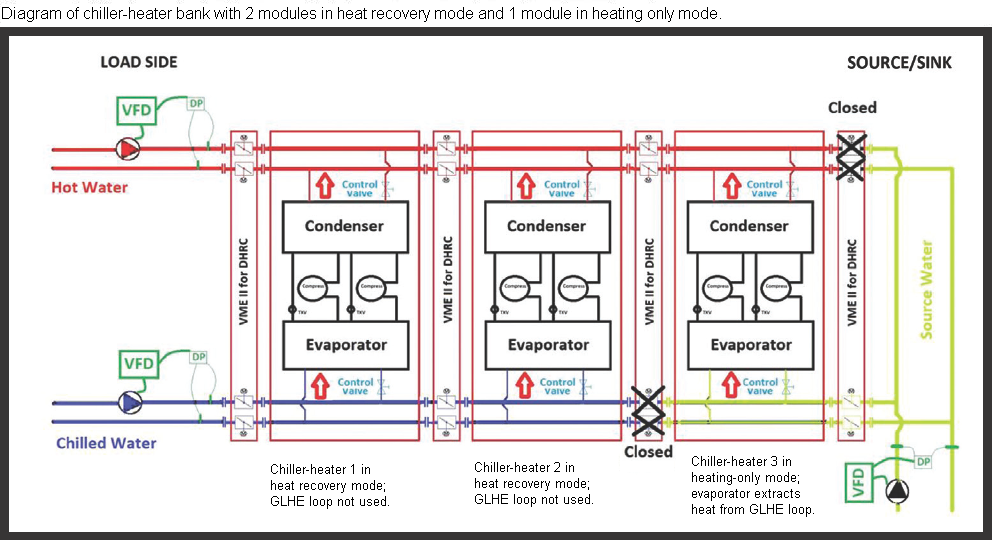
\includegraphics[width=0.9\textwidth, height=0.9\textheight, keepaspectratio=true]{media/image188.png}
\caption{Diagram of a central heat pump system with two chiller-heaters in heat recovery mode and one chiller-heater in heating-only mode \protect \label{fig:diagram-of-a-central-heat-pump-system-with-003}}
\end{figure}

In the above example, the heating load needs 3 chiller-heaters and the cooling load needs two chiller-heaters. Chillers 1 and 2 are in heat recovery mode and isolated from the ground source loop while chiller 3 is in heating-only mode, its evaporator extracting heat from the ground source loop.

Users are required to define three different nodes such as chilled water, hot water, and source water nodes. Only this central heat pump system will be metered, and individual chiller-heaters' energy will be available for reporting only, but not metered.

\subsubsection{Inputs}\label{inputs-19-004}

\paragraph{Field: Name}\label{field-name-18-005}

This alpha field contains the identifying name of the central heat pump system.

\paragraph{Field: Control Method}\label{field-control-method}

\paragraph{This field must contain a keyword defines how the central heat pump system controls the interaction between the chiller-heater modules and the water loops to meet the cooling and heating demands. Currently, the only available option isSmartMixing.}\label{this-field-must-contain-a-keyword-defines-how-the-central-heat-pump-system-controls-the-interaction-between-the-chiller-heater-modules-and-the-water-loops-to-meet-the-cooling-and-heating-demands.-currently-the-only-available-option-issmartmixing.}

\paragraph{Field: Cooling Loop Inlet Node Name}\label{field-cooling-loop-inlet-node-name}

This alpha field contains the identifying name of the chilled water inlet node.

\paragraph{Field: Cooling Loop Outlet Node Name}\label{field-cooling-loop-outlet-node-name}

This alpha field contains the identifying name of the chilled water outlet node.

\paragraph{Field: Source Loop Inlet Node Name}\label{field-source-loop-inlet-node-name}

This alpha field contains the identifying name of the source water inlet node.

\paragraph{Field: Source Loop Outlet Node Name}\label{field-source-loop-outlet-node-name}

This alpha field contains the identifying name of the source water outlet node.

\paragraph{Field: Heating Loop Inlet Node Name}\label{field-heating-loop-inlet-node-name}

This alpha field contains the identifying name of the hot water inlet node.

\paragraph{Field: Heating Loop Outlet Node Name}\label{field-heating-loop-outlet-node-name}

This alpha field contains the identifying name of the hot water outlet node.

\paragraph{Field: Ancillary Power}\label{field-ancillary-power-000}

This numeric field contains the ancillary power of the central heat pump system in watts.

\paragraph{Field: Ancillary Operation Schedule Name}\label{field-ancillary-operation-schedule-name}

This alpha field contains the identifying name of the ancillary power schedule.

\paragraph{Field Set: Individual Chiller-Heater Module Objects}\label{field-set-individual-chiller-heater-module-objects}

The following four items are repeated up to a maximum of 20 individual chiller-heater modulesets. At least one module set must appear in an input file. In other words, a central heat pump system must include at least one chiller-heater module component. A set of the following four fields helps to define the specific type of a chiller-heater module, its operation control, and the number of identical chiller-heater module objects.

\paragraph{Field: Chiller Heater Module Performance Component Object Type \textless{}x\textgreater{}}\label{field-chiller-heater-module-performance-component-object-type-x}

This alpha field describes the type of the chiller-heater comprising this module set. Only the chiller-heater type ChillerHeaterPerformance:EIectric:EIR is currently available. Note that up to 20 sets of chiller-heater module name, schedule, and number of identical chiller-heater may be entered for a single central heat pump system.

\paragraph{Field: Chiller Heater Module Performance Component Name \textless{}x\textgreater{}}\label{field-chiller-heater-module-performance-component-name-x}

This alpha field is paired with the preceding chiller-heater module type to define the name of the module.

\paragraph{Field: Chiller Heater Module Control Schedule Name \textless{}x\textgreater{}}\label{field-chiller-heater-module-control-schedule-name-x}

This alpha field is paired with the preceding chiller-heater module type and name to define its on/off control. This schedule will be used for all identical module components as defined in the next field. Currently, this schedule only controls the module set's availability, i.e., schedule values equal to 1 indicate that the chiller-heater set is available while schedule values equal to 0 indicate that the chiller-heater set is off.

\paragraph{Field: Number of Chiller Heater Modules \textless{}x\textgreater{}}\label{field-number-of-chiller-heater-modules-x}

This numeric field is paired with the preceding three fields to define how many identical chiller-heaters define this module set.

An example of this statement in an IDF is:

\begin{lstlisting}

CentralHeatPumpSystem,
    ChillerBank,             !- Name
    SmartMixing,             !- Control Method
    Chiller Inlet Node,      !- Cooling Loop Inlet Node Name
    Chiller Outlet Node,     !- Cooling Loop Outlet Node Name
    Condenser Inlet Node,    !- Source Loop Inlet Node Name
    Condenser Outlet Node,   !- Source Loop Outlet Node Name
    HWInlet,                 !- Heating Loop Inlet Node Name
    HWOutlet,                !- Heating Loop Outlet Node Name
    460,                     !- Ancillary Power {W}
    ,                        !- Ancillary Operation Schedule Name
    ChillerHeaterPerformance:Electric:EIR,  !- Chiller Heater Modules Object Type 1
    ChillerHeaterModule 1,   !- Chiller Heater Modules Performance Component Name 1
    ON,                      !- Chiller Heater Modules Control Schedule Name 1
    2,                       !- Number of Chiller Heater Modules 1
    ChillerHeaterPerformance:Electric:EIR,  !- Chiller Heater Modules Object Type 2
    ChillerHeaterModule 2,   !- Chiller Heater Modules Performance Component Name 2
    ON,                      !- Chiller Heater Modules Control Schedule Name 2
    2;                       !- Number of Chiller Heater Modules 2
\end{lstlisting}

\subsubsection{Outputs}\label{outputs-17-000}

\begin{itemize}
\item
  HVAC,Average,Chiller Heater System Cooling Electric Power {[}W{]}
\item
  HVAC,Sum,Chiller Heater System Cooling Electric Energy{[}J{]}
\item
  HVAC,Average,Chiller Heater System Heating Electric Power {[}W{]}
\item
  HVAC,Sum,Chiller Heater System Heating Electric Energy{[}J{]}
\item
  HVAC,Average,Chiller Heater System Cooling Rate {[}W{]}
\item
  HVAC,Sum,Chiller Heater System Cooling Energy{[}J{]}
\item
  HVAC,Average,Chiller Heater System Heating Rate {[}W{]}
\item
  HVAC,Sum,Chiller Heater System Heating Energy{[}J{]}
\item
  HVAC,Average,Chiller Heater System Source Heat Transfer Rate {[}W{]}
\item
  HVAC,Sum,Chiller Heater System Source Heat Transfer Energy{[}J{]}
\item
  HVAC,Average,Chiller Heater System Cooling Inlet Temperature {[}C{]}
\item
  HVAC,Average,Chiller Heater System Cooling Outlet Temperature {[}C{]}
\item
  HVAC,Average,Chiller Heater System Cooling Mass Flow Rate {[}kg/s{]}
\item
  HVAC,Average,Chiller Heater System Heating Inlet Temperature {[}C{]}
\item
  HVAC,Average,Chiller Heater System Heating Outlet Temperature {[}C{]}
\item
  HVAC,Average,Chiller Heater System Heating Mass Flow Rate {[}kg/s{]}
\item
  HVAC,Average,Chiller Heater System Source Inlet Temperature {[}C{]}
\item
  HVAC,Average,Chiller Heater System Source Outlet Temperature {[}C{]}
\item
  HVAC,Average,Chiller Heater System Source Mass Flow Rate {[}kg/s{]}
\end{itemize}

\paragraph{Chiller Heater System Cooling Electric Power {[}W{]}}\label{chiller-heater-system-cooling-electric-power-w}

\paragraph{Chiller Heater System Cooling Electric Energy {[}J{]}}\label{chiller-heater-system-cooling-electric-energy-j}

These outputs are the sums of the cooling electric power consumption of the central heat pump system containing one or more child objects. Cooling Energy is metered on Cooling:Electricity, Electricity:Plant, and Electricity:Facility.

\paragraph{Chiller Heater System Heating Electric Power {[}W{]}}\label{chiller-heater-system-heating-electric-power-w}

\paragraph{Chiller Heater System Heating Electric Energy {[}J{]}}\label{chiller-heater-system-heating-electric-energy-j}

These outputs are the sums of the heating electric power consumption of the central heat pump system. Heating Energy is metered on Heating:Electricity, Electricity:Plant, and Electricity:Facility.

\paragraph{Chiller Heater System Cooling Rate {[}W{]}}\label{chiller-heater-system-cooling-rate-w}

\paragraph{Chiller Heater System Cooling Energy {[}J{]}}\label{chiller-heater-system-cooling-energy-j}

These outputs are the evaporator heat transfer which is the cooling delivered by the central heat pump system. These are the sums of the evaporator heat transfer of individual chiller-heater modules included in the central heat pump system. Cooling Energy is metered on Chiller:EnergyTransfer, EnergyTransfer:Plant, and EnergyTransfer:Facility.

\paragraph{Chiller Heater System Heating Rate {[}W{]}}\label{chiller-heater-system-heating-rate-w}

\paragraph{Chiller Heater System Heating Energy {[}J{]}}\label{chiller-heater-system-heating-energy-j}

These outputs are the condenser heat transfer which is the heating delivered by the central heat pump system. These are the sums of the condenser heat transfer of individual chiller-heater modules included in the central heat pump system. Heating Energy is metered on Boiler:EnergyTransfer, EnergyTransfer:Plant, and EnergyTransfer:Facility.

\paragraph{Chiller Heater System Source Heat Transfer Rate {[}W{]}}\label{chiller-heater-system-source-heat-transfer-rate-w}

\paragraph{Chiller Heater System Source Heat Transfer Energy {[}J{]}}\label{chiller-heater-system-source-heat-transfer-energy-j}

These outputs are heat transfer which is the heat rejected to a ground source loop or extracted from the source loop, depending on the operating modes of the chiller-heater modules. This is the sums of evaporator heat transfer of the chiller-heater modules in heating-only mode or heating dominant simultaneous cooling-heating mode while the sums of condenser heat transfer of the chiller-heater modules in cooling-only mode or cooling dominant simultaneous cooling-heating mode. Source Heat Transfer Energy is metered on HeatRejection:EnergyTransfer, EnergyTransfer:Plant, and EnergyTransfer:Facility.

\paragraph{Chiller Heater System Cooling Inlet Temperature {[}C{]}}\label{chiller-heater-system-cooling-inlet-temperature-c}

\paragraph{Chiller Heater System Cooling Outlet Temperature {[}C{]}}\label{chiller-heater-system-cooling-outlet-temperature-c}

\paragraph{Chiller Heater System Cooling Mass Flow Rate {[}kg/s{]}}\label{chiller-heater-system-cooling-mass-flow-rate-kgs}

These outputs are the chilled water inlet and outlet temperatures and flow rate.

\paragraph{Chiller Heater System Heating Inlet Temperature {[}C{]}}\label{chiller-heater-system-heating-inlet-temperature-c}

\paragraph{Chiller Heater System Heating Outlet Temperature {[}C{]}}\label{chiller-heater-system-heating-outlet-temperature-c}

\paragraph{Chiller Heater System Heating Mass Flow Rate {[}kg/s{]}}\label{chiller-heater-system-heating-mass-flow-rate-kgs}

These outputs are the hot water inlet and outlet temperatures and flow rate.

\paragraph{Chiller Heater System Source Inlet Temperature {[}C{]}}\label{chiller-heater-system-source-inlet-temperature-c}

\paragraph{Chiller Heater System Source Outlet Temperature {[}C{]}}\label{chiller-heater-system-source-outlet-temperature-c}

\paragraph{Chiller Heater System Source Mass Flow Rate {[}kg/s{]}}\label{chiller-heater-system-source-mass-flow-rate-kgs}

These outputs are the source water inlet and outlet temperatures and flow rate.

\subsection{ChillerHeaterPerformance:EIectric:EIR}\label{chillerheaterperformanceeiectriceir}

The performance of the chiller-heater will be defined by two sets of curves meant to describe unloading for: 1) cooling-only mode, and 2) heating-only mode or simultaneous cooling-heating mode. Reference conditions must be defined for both because each has its own set of three unloading curves based on their associated reference conditions. The cooling-mode curves are typically (but not always) based on condenser entering water temperature while the heating-only mode curves are typically based on condenser leaving water temperature. This chiller-heater object allows the user to specify whether to use condenser leaving or condenser entering as a dependent variable to differentiate, if necessary, the condenser temperature basis used to generate the cooling- and heating-only mode curves.

\subsubsection{Field: Name}\label{field-name-19-002}

This alpha field contains the identifying name of the chiller-heater to be included in a central heat pump system.

\subsubsection{Field: Reference Cooling Mode Evaporator Capacity}\label{field-reference-cooling-mode-evaporator-capacity}

This numeric field contains the reference cooling capacity of the evaporator in cooling mode in Watts. This value should be based on the reference temperatures and design water flow rates defined below. This field can be autosized.

\subsubsection{Field: Reference Cooling Mode COP}\label{field-reference-cooling-mode-cop}

This numeric field contains the reference coefficient of performance of the evaporator for cooling. It must be based on the values of Reference Cooling Mode Leaving Chilled Water Temperature and Reference Cooling Mode Entering Condenser Water Temperature defined in the next two fields.

\subsubsection{Field: Reference Cooling Mode Leaving Chilled Water Temperature}\label{field-reference-cooling-mode-leaving-chilled-water-temperature}

This numeric field contains the reference leaving chilled water temperature of the evaporator for cooling in Celsius. The default value is 6.67°C.

\subsubsection{Field: Reference Cooling Mode Entering Condenser Water Temperature}\label{field-reference-cooling-mode-entering-condenser-water-temperature}

This numeric field contains the reference entering condenser water temperature of the condenser in the cooling mode in Celsius. The default value is 29.4°C.

\subsubsection{Field: Reference Cooling Mode Leaving Condenser Water Temperature}\label{field-reference-cooling-mode-leaving-condenser-water-temperature}

This numeric field contains the reference leaving condenser water temperature of the condenser in the cooling mode in Celsius. The default value is 35.0°C.

\subsubsection{Field: Reference Heating Mode Cooling Capacity Ratio}\label{field-reference-heating-mode-cooling-capacity-ratio}

This numeric field contains the evaporator's capacity during the reference heating-only or simultaneous cooling-heating mode as a ratio of reference cooling capacity. For example, the ratio may be expressed as follows:

\begin{equation}
Ratio = \frac{{EvapCapHt{g_{@Tchw,l = 6.67C,Tcond,l = 51.67C}}}}{{EvapCapC{{\lg }_{@Tchw,l = 6.67C,Tcond,l = 35.0C}}}}
\end{equation}

where Tchw,l is the leaving chilled water temperature and Tcond,l is the leaving condenser water temperature representing the heating-mode and cooling-mode reference temperatures defined elsewhere in this object.

The default is 0.75. This field is used to determine evaporator capacity in heating-only mode or simultaneous cooling-heating mode, multiplying it by the value entered in the field of the Reference Cooling Mode Evaporator Capacity. Note that even when there is no cooling load, i.e., the machine is in heating-only mode, the evaporator must still run and extract heat from the source water. In heating-only mode, the leaving chilled water temperature (Tchw,l) may ~float depending on the evaporator water flow rate and the source water temperature. In simultaneous cooling and heating mode, the leaving chilled water temperature (Tchw,l) does not float but is determined by the chilled water setpoint controls. For both heating-only and simultaneous cooling and heating mode, the leaving condenser temperature (Tcond,l) is determined by the hot water supply setpoint controls. This value of Tchw,l, combined with Tcond,l is plugged into the CAPFT and EIRFT curves to determine the off-rated heating-mode evaporator capacity and associated compressor power.

\subsubsection{Field: Reference Heating Mode Cooling Power Ratio}\label{field-reference-heating-mode-cooling-power-ratio}

This numeric field contains the compressor power during simultaneous cooling-heating mode as a ratio of reference cooling compressor power. For example, the ratio may be expressed as follows:

\begin{equation}
Ratio = \frac{{Powe{r_{@Tchw,l = 6.67C,Tcond,l = 51.67C}}}}{{Powe{r_{@Tchw,l = 6.67C,Tcond,l = 35.0C}}}}
\end{equation}

The default value is 1.5. This field is used to determine full load compressor power at the simultaneous cooling-heating mode's reference chilled water leaving and condenser water leaving temperatures. Note: In heating-only mode, the chilled water leaving temperature floats so the EIRFT curve is used to modify the simultaneouos cooling-heating full load compressor power value.

\subsubsection{Field: Reference Heating Mode Leaving Chilled Water Temperature}\label{field-reference-heating-mode-leaving-chilled-water-temperature}

This numeric field contains the reference leaving chilled water temperature of the evaporator in simultaneous cooling-heating mode in Celsius. This is typically the same as the reference cooling mode value and is used to create the heating-only mode and simultaneous cooling-heating mode unloading curves. The leaving chilled water temperature for the chiller-heater is not allowed to fall below this value during the heating-only mode and simultaneous cooling-heating mode. The default value is 6.67°C.

\subsubsection{Field: Reference Heating Mode Leaving Condenser Water Temperature}\label{field-reference-heating-mode-leaving-condenser-water-temperature}

This numeric field contains the reference leaving condenser water temperature of the condenser in heating mode in Celsius. This field is typically controlled to the design hot water supply temperature, and used to create the heating-only mode and simultaneous cooling-heating mode unloading curves. The default value is 60.0°C.

\subsubsection{Field: Reference Heating Mode Entering Condenser Water Temperature}\label{field-reference-heating-mode-entering-condenser-water-temperature}

This numeric field contains the reference entering condenser water temperature of the condenser in heating mode in Celsius. This field typically represents the upper limit of the source water temperature. The default value is 29.44°C.

\subsubsection{Field: Heating Mode Entering Chilled Water Temperature Low Limit}\label{field-heating-mode-entering-chilled-water-temperature-low-limit}

This numeric field contains the low limit of the entering chilled water temperature in heating-only mode or simultaneous cooling-heating mode in Celsius. This field typically represents the lower limit of the source water temperature. If necessary, auxiliary heat will be activated to prevent source water temperature falling below the chilled water entering minimum. The default value is 12.2°C.

\subsubsection{Field: Chilled Water Flow Mode Type}\label{field-chilled-water-flow-mode-type}

This alpha field contains the chilled water flow control mode. Valid water flow mode includes constant flow and variable flow, and the default water flow mode is constant flow.

\subsubsection{Field: Design Chilled Water Flow Rate}\label{field-design-chilled-water-flow-rate-8}

This numeric field contains the design chilled water flow rate in m\(^{3}\)/s. The minimum value for this field must be greater than zero, and this field is autosizable.

\subsubsection{Field: Design Condenser Water Flow Rate}\label{field-design-condenser-water-flow-rate-7}

This numeric field contains the design condenser water flow rate in m\(^{3}\)/s. The minimum value for this field must be greater than zero, and this field is autosizable.

\subsubsection{Field: Design Hot Water Flow Rate}\label{field-design-hot-water-flow-rate-2}

This numeric field contains the design hot water flow rate in m\(^{3}\)/s. The minimum value and default value for this field are zero, and this field is autosizable.

\subsubsection{Field: Compressor Motor Efficiency}\label{field-compressor-motor-efficiency}

This numeric field contains the fraction of efficiency of the compressor electrical energy consumption that must be rejected by the condenser. This value must be between 0.0 and 1.0, and the default value is 1.0.

\subsubsection{Field: Condenser Type}\label{field-condenser-type-7}

This alpha field contains the type of condenser. WaterCooled is the only valid type, and it requires the full specification of the condenser loop and its associated equipment.

\subsubsection{Field: Cooling Mode Temperature Curve Condenser Water Independent Variable}\label{field-cooling-mode-temperature-curve-condenser-water-independent-variable}

This alpha field determines whether the entering or leaving condenser water temperature is used in the cooling mode unloading performance curves that follow. Valid variables include EnteringCondenser and LeavingCondenser, and the default variable is EnteringCondenser. The condenser temperature used for the cooling mode unloading performance curves will be dependent on this field input. For example, leaving condenser water temperature will be used when the LeavingCondenser is chosen, otherwise entering condenser water temperature.

\subsubsection{Field: Cooling Mode Cooling Capacity Function of Temperature Curve Name}\label{field-cooling-mode-cooling-capacity-function-of-temperature-curve-name}

This alpha field contains the name of a biquadratic performance curve (ref: Performance Curves) that parameterizes the variation of the evaporator capacity as a function of the leaving chilled water temperature and either the entering condenser water temperature or the leaving condenser water temperature as defined in the previous field. It is then multiplied by the reference evaporator capacity to give the cooling capacity at specific temperature operating conditions (i.e., at temperatures different from the reference temperatures). The curve should have a value of 1.0 at the reference temperatures and flow rates specified above. The biquadratic curve should be valid for the range of water temperatures anticipated for the simulation.

\subsubsection{Field: Cooling Mode Electric Input to Cooling Output Ratio Function of Temperature Curve Name}\label{field-cooling-mode-electric-input-to-cooling-output-ratio-function-of-temperature-curve-name}

This alpha field contains the name of a biquadratic performance curve (ref: Performance Curves) that parameterizes the variation of the energy input to cooling output ratio (EIR) as a function of the leaving chilled water temperature and either the entering condenser water temperature or the leaving condenser water temperature as defined by the user. The EIR is the inverse of the COP. It is then multiplied by the reference EIR (inverse of the reference COP) to give the EIR at specific temperature operating conditions (i.e., at temperatures different from the reference temperatures). The curve should have a value of 1.0 at the reference temperatures and flow rates specified above. The biquadratic curve should be valid for the range of water temperatures anticipated for the simulation.

\subsubsection{Field: Cooling Mode Electric Input to Cooling Output Ratio Function of Part Load Ratio Curve Name}\label{field-cooling-mode-electric-input-to-cooling-output-ratio-function-of-part-load-ratio-curve-name}

This alpha field contains the name of a performance curve (ref: Performance Curves) that parameterizes the variation of the energy input to cooling output ratio (EIR) as a function of the part-load ratio (EIRFPLR). The EIR is the inverse of the COP, and the part-load ratio is the actual cooling load divided by the available cooling capacity of the chiller-heater. This curve is generated by dividing the operating electric input power by the available full-load capacity at the specific operating temperatures. The curve output should decrease from 1 towards 0 as part-load ratio decreases from 1 to 0. Note that the bi-cubic formulation is generally only valid when LeavingCondenser variable is chosen for the field of Cooling Mode Condenser Water Temperature Curve Input Variable whereas the quadratic curve can be used both choices, i.e., LeavingCondenser and EnteringCondenser. The output of this curve is then multiplied by the reference full-load EIR and the EIRFT to give the EIR at the specific temperatures and part-load ratio at which the chiller-heater is operating. This curve should have a value of 1.0 when the part-load ratio equals 1.0. The curve should be valid for the range of part-load ratios anticipated for the simulation.

\subsubsection{Field: Cooling Mode Cooling Capacity Optimum Part Load Ratio}\label{field-cooling-mode-cooling-capacity-optimum-part-load-ratio}

This numeric field contains the chiller-heater's optimum part-load ratio. This is the part-load ratio at which the chiller-heater performs at its maximum COP. The optimum part-load ratio must be greater than or equal to the minimum part-load ratio, and less than or equal to the maximum part-load ratio. (Note: Both the minimum part-load ratio and maximum part-load ratio are taken from the Cooling Mode EIRFPLR curve definition.) The default value is 1.0.

\subsubsection{Field: Heating Mode Temperature Curve Condenser Water Independent Variable}\label{field-heating-mode-temperature-curve-condenser-water-independent-variable}

This alpha field determines whether the entering or leaving condenser water temperature is used in the heating mode unloading performance curves that follow. Valid variables include EnteringCondenser and LeavingCondenser, and the default variable is EnteringCondenser. The condenser temperature used for the cooling mode unloading performance curves will be dependent on this field input. For example, leaving condenser water temperature will be used when the LeavingCondenser is chosen, otherwise entering condenser water temperature.

\subsubsection{Field: Heating Mode Cooling Capacity Function of Temperature Curve Name}\label{field-heating-mode-cooling-capacity-function-of-temperature-curve-name}

This alpha field contains the name of a biquadratic performance curve (ref: Performance Curves) that parameterizes the variation of the evaporator capacity in heating mode as a function of the leaving chilled water temperature and either the entering condenser water temperature or the leaving condenser water temperature as defined in the previous field. This curve is used to evaluate the adjusted evaporator capacity during heating-only mode or simultaneous cooling-heating mode. This adjusted capacity is used as part of the cooling part-load calculation for the EIRFPLR curve. It is then multiplied by the reference evaporator capacity to give the cooling capacity at specific temperature operating conditions (i.e., at temperatures different from the reference temperatures). The curve should have a value of 1.0 at the reference temperatures and flow rates specified above. The biquadratic curve should be valid for the range of water temperatures anticipated for the simulation.

\subsubsection{Field: Heating Mode Electric Input to Cooling Output Ratio Function of Temperature Curve Name}\label{field-heating-mode-electric-input-to-cooling-output-ratio-function-of-temperature-curve-name}

This alpha field contains the name of a biquadratic performance curve (ref: Performance Curves) that parameterizes the variation of the energy input to cooling output ratio (EIR) as a function of the leaving chilled water temperature and either the entering condenser water temperature or the leaving condenser water temperature as defined by the user. The EIR is the inverse of the COP. It is then multiplied by the reference EIR (inverse of the reference COP) to give the EIR at specific temperature operating conditions (i.e., at temperatures different from the reference temperatures). The curve should have a value of 1.0 at the reference temperatures and flow rates specified above. The biquadratic curve should be valid for the range of water temperatures anticipated for the simulation.

\subsubsection{Field: Heating Mode Electric Input to Cooling Output Ratio Function of Part Load Ratio Curve Name}\label{field-heating-mode-electric-input-to-cooling-output-ratio-function-of-part-load-ratio-curve-name}

This alpha field contains the name of a performance curve (ref: Performance Curves) that parameterizes the variation of the energy input to cooling output ratio (EIR) as a function of the part-load ratio (EIRFPLR). The EIR is the inverse of the COP, and the part-load ratio is the actual evaporator load divided by the available evaporator capacity of the chiller-heater at the reference heating and simultaneous cooling-heating mode temperatures. This curve is generated by dividing the operating electric input power by the available full-load capacity (do not divide by load) at the specific operating temperatures. The curve output should decrease from 1 towards 0 as part-load ratio decreases from 1 to 0. Note that the bicubic formulation below can only be used when the chiller-heater uses a variable speed compressor motor drive. It is also generally valid only when LeavingCondenser variable is chosen for the field of Cooling Mode Condenser Water Temperature Curve Input Variable whereas the quadratic curve can be used both choices, i.e., LeavingCondenser and EnteringCondenser. The output of this curve is then multiplied by the reference full-load EIR (inverse of the reference COP) and the EIRFT to give the EIR at the specific temperatures and part-load ratio at which the chiller-heater is operating. This curve should have a value of 1.0 when the part-load ratio equals 1.0. The curve should be valid for the range of part-load ratios anticipated for the simulation.

\subsubsection{Field: Heating Mode Cooling Capacity Optimum Part Load Ratio}\label{field-heating-mode-cooling-capacity-optimum-part-load-ratio}

This numeric field contains the chiller-heater's optimum part-load ratio during heating-only mode or simultaneous cooling-heating mode. This is the part-load ratio at which the chiller-heater performs at its maximum COP. The optimum part-load ratio must be greater than or equal to the minimum part-load ratio, and less than or equal to the maximum part-load ratio. (Note: Both the minimum part-load ratio and maximum part-load ratio are taken from the Heating Mode EIRFPLR curve definition.) The default value is 1.0.

\subsubsection{Field: Sizing Factor}\label{field-sizing-factor-12}

This optional numeric field allows the user to specify a sizing factor for this component. The Sizing Factor is a multiplier on the design plant chilled water loop flow rate associated with the chiller-heaters parent CentralHeatPumpSystem object. The chiller-heater's modified chilled water flow can then be used to autocalculate the Design Condenser Water Flow Rate and Reference Cooling Mode Evaporator Capacity values. In general, it is best to autosize all three fields or set fixed values for all three fields.

An example of this statement in an IDF is:

\begin{lstlisting}

ChillerHeaterPerformance:Electric:EIR,
    ChillerHeaterModule 1,   !- Name
    12500,                   !- Reference Cooling Mode Evaporator Capacity {W}
    1.5,                     !- Reference Cooling Mode COP {W/W}
    6.67,                    !- Reference Cooling Mode Leaving Chilled Water Temperature {C}
    29.4,                    !- Reference Cooling Mode Entering Condenser Fluid Temperature {C}
    35.0,                    !- Reference Cooling Mode Leaving Condenser Water Temperature {C}
    0.74,                    !- Reference Heating Mode Cooling Capacity Ratio
    1.38,                    !- Reference Heating Mode Cooling Power Input Ratio
    6.67,                    !- Reference Heating Mode Leaving Chilled Water Temperature {C}
    60,                      !- Reference Heating Mode Leaving Condenser Water Temperature {C}
    29.44,                   !- Reference Heating Mode Entering Condenser Fluid Temperature {C}
    5,                       !- Heating Mode Entering Chilled Water Temperature Low Limit {C}
    VariableFlow,            !- Chilled Water Flow Mode Type
    0.0003525,               !- Design Chilled Water Flow Rate {m$^{3}$/s}
    0.0005525,               !- Design Condenser Water Flow Rate {m$^{3}$/s}
    0.0003525,               !- Design Hot Water Flow Rate {m$^{3}$/s}
    1,                       !- Compressor Motor Efficiency
    WaterCooled,             !- Condenser Type
    EnteringCondenser,       !- Cooling Mode Temperature Curve Condenser Water Independent Variable
    ChillerHeaterClgCapFT,   !- Cooling Mode Cooling Capacity Function of Temperature Curve Name
    ChillerHeaterClgEIRFT,   !- Cooling Mode Electric Input to Cooling Output Ratio Function of
                                !-   Temperature Curve Name
    ChillerHeaterClgEIRFPLR, !- Cooling Mode Electric Input to Cooling Output Ratio Function of Part Load
                         !-   Ratio Curve Name
    1,                       !- Cooling Mode Cooling Capacity Optimum Part Load Ratio
    LeavingCondenser,        !- Heating Mode Temperature Curve Condenser Water Independent Variable
    ChillerHeaterHtgCapFT,   !- Heating Mode Cooling Capacity Function of Temperature Curve Name
    ChillerHeaterHtgEIRFT,   !- Heating Mode Electric Input to Cooling Output Ratio Function of
                               !-   Temperature Curve Name
    ChillerHeaterHtgEIRFPLR, !- Heating Mode Electric Input to Cooling Output Ratio Function of Part Load
                               !-   Ratio Curve Name
    1,                       !- Heating Mode Cooling Capacity Optimum Part Load Ratio
    1;                       !- Sizing Factor
\end{lstlisting}

\subsection{ChillerHeaterPerformance:Electric:EIR Outputs}\label{chillerheaterperformanceelectriceir-outputs}

\begin{itemize}
\item
  HVAC,Average,Chiller Heater Operation Mode Unit \textless{}x\textgreater{} {[]}
\item
  HVAC,Average,Chiller Heater Part Load Ratio Unit \textless{}x\textgreater{} {[]}
\item
  HVAC,Average,Chiller Heater Cycling Ratio Unit \textless{}x\textgreater{} {[]}
\item
  HVAC,Average,Chiller Heater Cooling Electric Power Unit \textless{}x\textgreater{} {[}W{]}
\item
  HVAC,Sum,Chiller Heater Cooling Electric Energy Unit \textless{}x\textgreater{} {[}J{]}
\item
  HVAC,Average,Chiller Heater Heating Electric Power Unit \textless{}x\textgreater{} {[}W{]}
\item
  HVAC,Sum,Chiller Heater Heating Electric Energy Unit \textless{}x\textgreater{} {[}J{]}
\item
  HVAC,Average,Chiller Heater Cooling Rate Unit \textless{}x\textgreater{} {[}W{]}
\item
  HVAC,Sum,Chiller Heater Cooling Energy Unit \textless{}x\textgreater{} {[}J{]}
\item
  HVAC,Average,Chiller Heater False Load Heat Transfer Rate Unit \textless{}x\textgreater{} {[}W{]}
\item
  HVAC,Sum,Chiller Heater False Load Heat Transfer Energy Unit \textless{}x\textgreater{} {[}J{]}
\item
  HVAC,Average,Chiller Heater Condenser Heat Transfer Rate Unit \textless{}x\textgreater{} {[}W{]}
\item
  HVAC,Sum,Chiller Heater Condenser Heat Transfer Energy Unit \textless{}x\textgreater{} {[}J{]}
\item
  HVAC,Average,Chiller Heater Evaporator Inlet Temperature Unit \textless{}x\textgreater{} {[}C{]}
\item
  HVAC,Average,Chiller Heater Evaporator Outlet Temperature Unit \textless{}x\textgreater{} {[}C{]}
\item
  HVAC,Average,Chiller Heater Evaporator Mass Flow Rate Unit \textless{}x\textgreater{} {[}kg/s{]}
\item
  HVAC,Average,Chiller Heater Condenser Inlet Temperature Unit \textless{}x\textgreater{} {[}C{]}
\item
  HVAC,Average,Chiller Heater Condenser Outlet Temperature Unit \textless{}x\textgreater{} {[}C{]}
\item
  HVAC,Average,Chiller Heater Condenser Mass Flow Rate Unit \textless{}x\textgreater{} {[}kg/s{]}
\item
  HVAC,Average,Chiller Heater COP Unit \textless{}x\textgreater{} {[]}
\item
  HVAC,Average,Chiller Heater Capacity Temperature Modifier Multiplier Unit \textless{}x\textgreater{} {[]}
\item
  HVAC,Average,Chiller Heater EIR Temperature Modifier Multiplier Unit \textless{}x\textgreater{} {[]}
\item
  HVAC,Average,Chiller Heater EIR Part Load Modifier Multiplier Unit \textless{}x\textgreater{} {[]}
\end{itemize}

Note that much of these output variables are adapted from the definitions above under ``Generic Chiller Outputs'' and ``Electric EIR Chiller Outputs.'' The following outputs are repeated up to the maximum of individual chiller-heater module objects. The maximum number may be different from the number of object defined in this object when users define two or more identical chiller-heater modules for a single chiller heater object in the central heat pump system.

\subsubsection{\texorpdfstring{Chiller Heater Operation Mode Unit \textless{}x\textgreater{} \protect\hyperlink{section-1}{~}}{Chiller Heater Operation Mode Unit \textless{}x\textgreater{} ~}}\label{chiller-heater-operation-mode-unit-x}

This output represents the operating mode of the chiller-heater module. Two single mode outputs and three simultaneous cooling-heating mode outputs are possible:

\begin{enumerate}
\def\labelenumi{\arabic{enumi}.}
\setcounter{enumi}{-1}
\item
  off
\item
  cooling-only mode
\item
  heating-only mode
\item
  heat recovery mode
\item
  cooling dominant simultaneous cooling-heating mode
\item
  heating dominant simultaneous cooling-heating mode.
\end{enumerate}

The first mode 0 is reported when the chiller-heater is turned off. The next two modes 2 and 3 are reported when the chiller-heater provides only either cooling or heating, respectively. The last three modes 3 to 5 indicate when the chiller-heater is in a simultaneous cooling-heating mode. Mode 3 indicates the chiller-heaters provides simultaneous cooling and heating \textbf{\emph{without}} heat exchange with the ground source. Mode 4 denotes that at least one of the chiller-heater modules in the central heat pump system provides both cooling and heating, and the chiller-heater is meeting remaining cooling demand (see Figure~\ref{fig:diagram-of-a-central-heat-pump-system-with-002}. Diagram of a central heat pump system with one chiller-heater in heat recovery mode and two chiller-heaters in cooling-only mode) Similarly, mode 5 indicates that at least one of the chiller-heater modules in the central heat pump system is in the heat recovery mode, and the chiller-heater is meeting remaining heating demand (see Figure~\ref{fig:diagram-of-a-central-heat-pump-system-with-003}).

Note that the decision to operate individual chiller-heater modules is solely dependent on the chiller-heater schedule and loads. A fraction may appear in case the chiller-heater mode varies within a zone time step. In this particular case, users may define a detailed reporting frequency for this output variable.

\subsubsection{\texorpdfstring{Chiller Heater Part Load Ratio Unit \textless{}x\textgreater{} \protect\hyperlink{section-1}{~}}{Chiller Heater Part Load Ratio Unit \textless{}x\textgreater{} ~}}\label{chiller-heater-part-load-ratio-unit-x}

This output is the ratio of the evaporator heat transfer rate plus the false load heat transfer rate (if applicable) to the available chiller-heater capacity. This value is used to determine ChillerEIRFPLR.

\subsubsection{\texorpdfstring{Chiller Heater Cycling Ratio Unit \textless{}x\textgreater{} \protect\hyperlink{section-1}{~}}{Chiller Heater Cycling Ratio Unit \textless{}x\textgreater{} ~}}\label{chiller-heater-cycling-ratio-unit-x}

The cycling ratio is the amount of time the chiller-heater operates during each simulation time step. If the chiller-heater part-load ratio falls below the minimum part-load ratio, the chiller-heater cycles on and off to meet the loads.

\subsubsection{Chiller Heater Cooling Electric Power Unit \textless{}x\textgreater{} {[}W{]}}\label{chiller-heater-cooling-electric-power-unit-x-w}

\subsubsection{Chiller Heater Cooling Electric Energy Unit \textless{}x\textgreater{} {[}J{]}}\label{chiller-heater-cooling-electric-energy-unit-x-j}

These outputs are the cooling electric power consumption of the chiller-heater.

\subsubsection{Chiller Heater Heating Electric Power Unit \textless{}x\textgreater{} {[}W{]}}\label{chiller-heater-heating-electric-power-unit-x-w}

\subsubsection{Chiller Heater Heating Electric Energy Unit \textless{}x\textgreater{} {[}J{]}}\label{chiller-heater-heating-electric-energy-unit-x-j}

These outputs are the heating electric power consumption of the chiller-heater.

\subsubsection{Chiller Heater Cooling Rate Unit \textless{}x\textgreater{} {[}W{]}}\label{chiller-heater-cooling-rate-unit-x-w}

\subsubsection{Chiller Heater Cooling Energy Unit \textless{}x\textgreater{} {[}J{]}}\label{chiller-heater-cooling-energy-unit-x-j}

These outputs are the evaporator heat transfer which is the cooling delivered by the chiller-heater module.

\subsubsection{Chiller Heater False Load Heat Transfer Rate Unit \textless{}x\textgreater{} {[}W{]}}\label{chiller-heater-false-load-heat-transfer-rate-unit-x-w}

\subsubsection{Chiller Heater False Load Heat Transfer Energy Unit \textless{}x\textgreater{} {[}J{]}}\label{chiller-heater-false-load-heat-transfer-energy-unit-x-j}

These outputs are the heat transfer rate and total heat transfer due to false loading of the chiller-heater. When the chiller-heater part-load ratio is below the minimum unloading ratio, the chiller-heater false loads (e.g.~hot-gas bypass) to further reduce capacity.

\subsubsection{Chiller Heater Condenser Heat Transfer Rate Unit \textless{}x\textgreater{} {[}C{]}}\label{chiller-heater-condenser-heat-transfer-rate-unit-x-c}

\subsubsection{Chiller Heater Condenser Heat Transfer Energy Unit \textless{}x\textgreater{} {[}C{]}}\label{chiller-heater-condenser-heat-transfer-energy-unit-x-c}

These outputs are the heat transfer which is the heating delivered by the chiller-heater module in heating mode.

\subsubsection{Chiller Heater Evaporator Inlet Temperature Unit \textless{}x\textgreater{} {[}C{]}}\label{chiller-heater-evaporator-inlet-temperature-unit-x-c}

\subsubsection{Chiller Heater Evaporator Outlet Temperature Unit \textless{}x\textgreater{} {[}C{]}}\label{chiller-heater-evaporator-outlet-temperature-unit-x-c}

\subsubsection{Chiller Heater Evaporator Mass Flow Rate Unit \textless{}x\textgreater{} {[}C{]}}\label{chiller-heater-evaporator-mass-flow-rate-unit-x-c}

These outputs are the evaporator water inlet and outlet temperatures and flow rate. Note that these represent the chilled water temperatures and flow rate in cooling mode or the source water temperature and flow rate in heating mode.

\subsubsection{Chiller Heater Condenser Inlet Temperature Unit \textless{}x\textgreater{} {[}C{]}}\label{chiller-heater-condenser-inlet-temperature-unit-x-c}

\subsubsection{Chiller Heater Condenser Outlet Temperature Unit \textless{}x\textgreater{} {[}C{]}}\label{chiller-heater-condenser-outlet-temperature-unit-x-c}

\subsubsection{Chiller Heater Condenser Mass Flow Rate Unit \textless{}x\textgreater{} {[}C{]}}\label{chiller-heater-condenser-mass-flow-rate-unit-x-c}

These outputs are the condenser water inlet and outlet temperatures and flow rate. Note that these represent the hot water temperatures and flow rate in heating mode or the source water temperature and flow rate in cooling mode.

\subsubsection{Chiller Heater COP Unit \textless{}x\textgreater{} {[}C{]}}\label{chiller-heater-cop-unit-x-c}

This output is the coefficient of performance for the chiller-heater. It is calculated as the evaporator heat transfer rate divided by the chiller-heater electric power.

\subsubsection{Chiller Heater Capacity Temperature Modifier Multiplier Unit \textless{}x\textgreater{} {[}C{]}}\label{chiller-heater-capacity-temperature-modifier-multiplier-unit-x-c}

This is the output of the curve object Cooling Capacity Function of Temperature Curve.

\subsubsection{Chiller Heater EIR Temperature Modifier Multiplier Unit \textless{}x\textgreater{} {[}C{]}}\label{chiller-heater-eir-temperature-modifier-multiplier-unit-x-c}

This is the output of the curve object Electric Input to Cooling Output Ratio Function of Temperature Curve.

\subsubsection{Chiller Heater EIR Part Load Modifier Multiplier Unit \textless{}x\textgreater{} {[}C{]}}\label{chiller-heater-eir-part-load-modifier-multiplier-unit-x-c}

This is the output of the curve object Electric Input to Cooling Output Ratio Function of Part Load Ratio Curve.

\subsection{Thermal Storage Objects}\label{thermal-storage-objects}

There are four types of cold thermal storage objects:

\begin{itemize}
\item
  ThermalStorage:Ice:Simple
\item
  ThermalStorage:Ice:Detailed
\item
  ThermalStorage:ChilledWater:Mixed
\item
  ThermalStorage:ChilledWater:Stratified
\end{itemize}

These objects are typically placed on the supply side of a primary chilled water loop in series or in parallel with one or more chillers.~ Using the the component set point (PlantEquipmentOperation:ComponentSetpoint) plant operation scheme type, the chiller and storage tank setpoints are used to control operation. Using a SetpointManager:Scheduled object (or other appropriate type of set point manager), the setpoints on the chiller outlet node and the ice storage outlet node can be used to control how the cooling load is shared and when charging of storage occurs.~ Example setpoints to use for various modes of operation are shown in the table below:

\begin{longtable}[c]{p{3.0in}p{1.5in}p{1.5in}}
\toprule 
Mode & Chiller Setpoint & Storage Setpoint \tabularnewline
\midrule
\endfirsthead

\toprule 
Mode & Chiller Setpoint & Storage Setpoint \tabularnewline
\midrule
\endhead

Charging ice storage tank & -5C & 7C \tabularnewline
Cooling with chiller only & 7C & 99C \tabularnewline
Cooling with chiller and storage (fully load chiller before using storage)) & 7C & 7C \tabularnewline
Cooling with chiller and storage (chiller carries portion of load, valid if chiller is upstream of storage) & 10C & 7C \tabularnewline
\bottomrule
\end{longtable}

Example files have been developed for three common storage configurations:

1.~Series -- Chiller Upstream:~ In this configuration, a chiller is placed first on the same branch as the storage unit and both use the \textbf{SeriesActive} branch control type.

2.~Series -- Chiller Downstream:~ In this configuration, a chiller is placed second on the same branch as the storage unit and both use the \textbf{SeriesActive} branch control type.

\begin{enumerate}
\def\labelenumi{\arabic{enumi}.}
\setcounter{enumi}{2}
\tightlist
\item
  Parallel:~ In this configuration, the chiller is on a branch parallel to the storage unit branch when it is not charging.~ During charging mode, valves will be changed so that the chiller is in series upstream of the storage.~ To accomplish this in EnergyPlus, the chiller must be modeled using two different chiller objects to represent the same chiller.~ One chiller object on a parallel branch operates only when storage is not being charged.~ The other chiller object, in series upstream of the storage unit operates only during charging mode.
\end{enumerate}

Other considerations for applying cold thermal storage objects include:

\begin{itemize}
\item
  In the PlantLoop object, the ``Minimum Loop Temperature'' must be set equal to or less than the lowest setpoint to be used anywhere in the loop.
\item
  To end the storage charging cycle, use a AvailabilityManager:LowTemperatureTurnOff to shut off the primary chilled water loop when the temperature leaving the storage tank nears the charging mode chiller setpoint indicating that the tank is fully charged.~ For example, if the chiller is set to provide --5C chilled water during charging, then charging can be shut down when the water temperature leaving the storage unit reaches --4C.~ When using a primary-secondary loop arrangement, it may be necessary to schedule this availability manager to be active only when the HVAC systems are off to avoid fighting between the demand controls and the availability manager.
\end{itemize}

\subsection{ThermalStorage:Ice:Simple}\label{thermalstorageicesimple}

This thermal storage model is based on a simple simulation of an ice storage tank with a fixed capacity.~ The tank is charged, or frozen, in an ice-on-coil configuration where ice builds up on the outside of the tubes carrying the brine or glycol solution from the chiller.~ There are two discharge (melt) options, internal or external.~ Internal melt uses the same fluid tubes for charging and discharging.~ External melt uses a separate fluid path for discharge such that the outer layers of ice melt first.~ The ice storage model includes an implied 3-way valve to control the amount if charge/discharge based on the incoming water temperature and the outlet node setpoint temperature.~ The storage tank is assumed to be fully charged (full of ice) at the beginning of each environment.~ The tank is then allowed to charge and discharge during the warmup days of the environment.~ The tank is best controlled using the PlantEquipmentOperation:ComponentSetpoint plant operation scheme, and requires that a setpoint be placed by a set point manager on the ice storage Plant Outlet Node.

The input fields for the object are described in detail below:

\subsubsection{Inputs}\label{inputs-20-004}

\paragraph{Field: Name}\label{field-name-20-001}

This alpha field contains the identifying name for the ice storage tank.

\paragraph{Field: Ice Storage Type}\label{field-ice-storage-type}

This alpha field specifies the type of ice storage tank to be modeled. There are two options:~ ``\textbf{IceOnCoilInternal}'' models ice-on-coil, internal melt.``IceOnCoilExternal'' models ice-on-coil, external melt.

\paragraph{Field: Capacity}\label{field-capacity-000}

This numeric field contains the nominal capacity of the ice storage in GJ (Giga is 10\(^{9}\)).

\paragraph{Field: Inlet Node Name}\label{field-inlet-node-name-004}

This alpha field specifies the name of the chilled water inlet node.

\paragraph{Field: Outlet Node Name}\label{field-outlet-node-name-005}

This alpha field specifies the name of the chilled water outlet node.

Following is an example input for the THERMAL STORAGE:ICE:SIMPLE object.

\begin{lstlisting}

ThermalStorage:Ice:Simple,
      ITS,                     !- Ice Storage Name
      IceOnCoilInternal,       !- Ice Storage Type
      1.5,                     !- Ice Storage Capacity {GJ}
      ITS Inlet Node,          !- Plant Loop Inlet Node
      ITS Outlet Node;         !- Plant Loop Outlet Node
\end{lstlisting}

\subsubsection{Outputs}\label{outputs-18-000}

The following outputs are available for simple Ice Storage model:

\begin{itemize}
\item
  HVAC,Average,Ice Thermal Storage Requested Load {[}W{]}
\item
  Zone,Average,Ice Thermal Storage End Fraction{[]}
\item
  HVAC,Average,Ice Thermal Storage Mass Flow Rate {[}kg/s{]}
\item
  HVAC,Average,Ice Thermal Storage Inlet Temperature {[}C{]}
\item
  HVAC,Average,Ice Thermal Storage Outlet Temperature {[}C{]}
\item
  HVAC,Average,Ice Thermal Storage Cooling Discharge Rate {[}W{]}
\item
  HVAC,Sum,Ice Thermal Storage Cooling Discharge Energy {[}J{]}
\item
  HVAC,Average,Ice Thermal Storage Cooling Charge Rate {[}W{]}
\item
  HVAC,Sum,Ice Thermal Storage Cooling Charge Energy {[}J{]}
\end{itemize}

\paragraph{Ice Thermal Storage Requested Load {[}W{]}}\label{ice-thermal-storage-requested-load-w}

The load requested by the plant control scheme. A positive value indicates a cooling load or a request to discharge (melt) the tank. A negative value indicates a request to charge (freeze) the tank.

\paragraph{\texorpdfstring{Ice Thermal Storage End Fraction {[]}}{Ice Thermal Storage End Fraction }}\label{ice-thermal-storage-end-fraction}

The fraction of full ice storage which is present at the end of the current HVAC timestep. When reported at a frequency less than detailed, this value is averaged over the reporting period.

\paragraph{Ice Thermal Storage Mass Flow Rate {[}kg/s{]}}\label{ice-thermal-storage-mass-flow-rate-kgs}

The total water mass flow rate through the ice storage component. Because the component includes an implied 3-way valve, this flow may be all through the tank, all bypassed through the valve, or a mixture of both.

\paragraph{Ice Thermal Storage Inlet Temperature {[}C{]}}\label{ice-thermal-storage-inlet-temperature-c}

The water temperature entering the ice storage component.

\paragraph{Ice Thermal Storage Outlet Temperature {[}C{]}}\label{ice-thermal-storage-outlet-temperature-c}

The water temperature leaving the ice storage component.

\paragraph{Ice Thermal Storage Cooling Discharge Rate {[}W{]}}\label{ice-thermal-storage-cooling-discharge-rate-w}

The rate of cooling delivered by the ice storage component. A positive value indicates the ice tank is discharging (melting). A zero value indicates the tank is charging or dormant.

\paragraph{Ice Thermal Storage Cooling Discharge Energy {[}J{]}}\label{ice-thermal-storage-cooling-discharge-energy-j}

The cooling energy delivered by the ice storage component. A positive value indicates the ice tank is discharging (melting). A zero value indicates the tank is charging or dormant.

\paragraph{Ice Thermal Storage Cooling Charge Rate {[}W{]}}\label{ice-thermal-storage-cooling-charge-rate-w}

The rate of charging delivered to the ice storage component. A positive value indicates the ice tank is charging (freezing). A zero value indicates the tank is discharging or dormant.

\paragraph{Ice Thermal Storage Cooling Charge Energy {[}J{]}}\label{ice-thermal-storage-cooling-charge-energy-j}

The charging energy delivered to the ice storage component. A positive value indicates the ice tank is charging (freezing). A zero value indicates the tank is discharging or dormant.

\subsection{ThermalStorage:Ice:Detailed}\label{thermalstorageicedetailed}

The detailed ice storage model allows the users of EnergyPlus to model more closely specific manufacturers' ice storage units. This is possible due to the use of curve fits to simulate the performance of the ice storage unit during charging and discharging. In this implementation, both charging and discharging are a function of the fraction charged/discharged as well as the log mean temperature difference across the storage unit. More information on the model is provided in the Engineering Reference for EnergyPlus. The remainder of this section describes the input required for the detailed ice storage model and the output that it can produce.

\subsubsection{Inputs}\label{inputs-21-004}

\paragraph{Field: Name}\label{field-name-21-001}

This field is the name of the detailed ice storage system given to it by the user.

\paragraph{Field: Availability Schedule Name}\label{field-availability-schedule-name-012}

This field is the name of the schedule (ref: Schedule) that determines whether or not the ice storage system is available during a particular time period. This allows the system to be turned off during a particular season. A value of less than or equal to zero indicates that the ice storage system is not available. Any value greater than zero indicates that the system is available. If this field is blank, the schedule has values of 1 for all time periods.

\paragraph{Field: Capacity}\label{field-capacity-1-000}

This number is the maximum amount of latent thermal storage available in the ice storage system. This model does not allow the removal or addition of sensible energy from the tank. Thus, it is always assumed to be at the freezing temperature of the storage material. The capacity is expressed in units of GJ.

\paragraph{Field: Inlet Node Name}\label{field-inlet-node-name-1-001}

This is the name of the node that connects the ice storage system to the plant loop. It is the inlet node to the ice storage component. The next field defines the outlet node. Due to presence of an internal bypass in this model, there are other ``nodes'' that are handled internally within the program. Users do not need to define any nodes other than the inlet and outlet nodes.

\paragraph{Field: Outlet Node Name}\label{field-outlet-node-name-1-002}

This is the name of the other node that connects the ice storage system to the plant loop. It is the outlet node to the ice storage component.

\paragraph{Field: Discharging Curve Object Type}\label{field-discharging-curve-object-type}

The detailed ice storage model in EnergyPlus takes advantage of the Curve feature of the program. Currently, the only two allowed curve fit types for the detailed ice storage model are the QuadraticLinear and the CubicLinear curves. More information on this curve can be found in the section on Curves.

\paragraph{Field: Discharging Curve Name}\label{field-discharging-curve-name}

This field specifies the name of the actual curve fit to be used to model the discharging process of the detailed ice storage system.

\paragraph{Field: Charging Curve Object Type}\label{field-charging-curve-object-type}

The detailed ice storage model in EnergyPlus takes advantage of the Curve feature of the program. Currently, the only two allowed curve fit types for the detailed ice storage model are the QuadraticLinear and the CubicLinear curves. More information on this curve can be found in the section on Curves.

\paragraph{Field: Charging Curve Name}\label{field-charging-curve-name}

This field specifies the name of the actual curve fit to be used to model the charging process of the detailed ice storage system.

\paragraph{Field: Timestep of the Curve Data}\label{field-timestep-of-the-curve-data}

This field defines what timestep was used to produce the curve fits named in the previous inputs. This parameter is important because the curve fit is non-dimensional. Thus, the data used to develop the curve fits were based on a specific length of time. In many cases, this is probably one hour or 1.0. The units for this parameter are hours.

\paragraph{Field: Parasitic Electric Load During Discharging}\label{field-parasitic-electric-load-during-discharging}

This field defines the amount of parasitic electric consumption (for controls or other miscellaneous electric consumption associate with the ice storage unit itself) during the discharge phase. This parameter is dimensionless and gets multiplied by the current load on the tank.

\paragraph{Field: Parasitic Electric Load During Charging}\label{field-parasitic-electric-load-during-charging}

This field defines the amount of parasitic electric consumption (for controls or other miscellaneous electric consumption associate with the ice storage unit itself) during the charge phase. This parameter is dimensionless and gets multiplied by the current load on the tank.

\paragraph{Field: Tank Loss Coefficient}\label{field-tank-loss-coefficient}

This field defines the loss of ice stored during a particular hour. This field is dimensionless (per hour). It is not multiplied by any temperature difference between the tank and the environment in which it might be located.

\paragraph{Field: Freezing Temperature of Storage Medium}\label{field-freezing-temperature-of-storage-medium}

This parameter defines the freezing/melting temperature of the ice storage medium in degrees Celsius. For most tanks, this is simply 0.0°C (the default value). However, some tanks may use other materials or salts which would change the freezing temperature. This can be changed using this parameter.

\paragraph{Field: Thaw Process Indicator}\label{field-thaw-process-indicator}

This input field assists in more accurate modeling of the charging process by defining how the thawing of ice takes place. There are two options for this input: \textbf{InsideMelt} and \textbf{OutsideMelt}. Some ice storage systems, by their nature, start the charging process with a bare coil or no ice left on the charging surface even though there is still ice stored in the tank.~ An example of such a system is sometimes referred to as an ice-on-coil inside melt system, and these systems would define this parameter using the ``InsideMelt'' option for this field.~ Other systems melt the ice from the outside, leaving ice still on the charging surface when charging begins. These systems are modeled using the ``OutsideMelt'' option.~ For systems that have a charging process that does not vary significantly with fraction charged can ignore this input by accepting the default value.~ The default value for this field is ``OutsideMelt''.

An IDF example:

\begin{lstlisting}

ThermalStorage:Ice:Detailed,
      Ice Tank,                !- Ice Storage Name
      ON,                      !- Ice Storage availability schedule
      0.5,                     !- Ice Storage Capacity {GJ}
      Ice Tank Inlet Node,     !- Plant Loop Inlet Node
      Ice Tank Outlet Node,    !- Plant Loop Outlet Node
      QuadraticLinear,         !- Discharging Curve Fit Type
      DischargeCurve,          !- Discharging Curve Name
      QuadraticLinear,         !- Charging Curve Fit Type
      ChargeCurve,             !- Charging Curve Name
      1.0,                     !- Timestep of Curve Fit Data
      0.0001,                  !- Parasitic electric load during discharging
      0.0002,                  !- Parasitic electric load during charging
      0.0003,                  !- Tank loss coefficient
      0.0;                     !- Freezing temperature [C]
\end{lstlisting}

\subsubsection{Outputs}\label{outputs-19-000}

Current detailed ice storage output variables are:

\begin{itemize}
\item
  System, Average, Ice Thermal Storage Cooling Rate {[}W{]}
\item
  System, Average, Ice Thermal Storage Change Fraction {[]}
\item
  System, Average, Ice Thermal Storage End Fraction {[]}
\item
  System, Average, Ice Thermal Storage Mass Flow Rate {[}kg/s{]}
\item
  System, Average, Ice Thermal Storage Bypass Mass Flow Rate {[}kg/s{]}
\item
  System, Average, Ice Thermal Storage Tank Mass Flow Rate {[}kg/s{]}
\item
  System, Average, Ice Thermal Storage Fluid Inlet Temperature {[}C{]}
\item
  System, Average, Ice Thermal Storage Blended Outlet Temperature {[}C{]}
\item
  System, Average, Ice Thermal Storage Tank Outlet Temperature {[}C{]}
\item
  System, Average, Ice Thermal Storage Cooling Discharge Rate {[}W{]}
\item
  System, Sum, Ice Thermal Storage Cooling Discharge Energy {[}J{]}
\item
  System, Average, Ice Thermal Storage Cooling Charge Rate {[}W{]}
\item
  System, Sum, Ice Thermal Storage Cooling Charge Energy {[}J{]}
\item
  System, Average, Ice Thermal Storage Ancillary Electric Power {[}W{]}
\item
  System, Sum, Ice Thermal Storage Ancillary Electric Energy {[}J{]}
\item
  System, Average, Ice Thermal Storage On Coil Fraction {[]}
\end{itemize}

\paragraph{~Ice Thermal Storage Cooling Rate {[}W{]}}\label{ice-thermal-storage-cooling-rate-w}

The actual load (absolute value) provided by the ice storage system during the current timestep

\paragraph{\texorpdfstring{Ice Thermal Storage Change Fraction {[]}}{Ice Thermal Storage Change Fraction }}\label{ice-thermal-storage-change-fraction}

The change in the ice tank's charge fraction charged during the current timestep (positive for charging, negative for discharging).

\paragraph{\texorpdfstring{Ice Thermal Storage End Fraction {[]}}{Ice Thermal Storage End Fraction }}\label{ice-thermal-storage-end-fraction-1}

The fraction charge of the ice storage system at the end of the timestep

\paragraph{\texorpdfstring{Ice Thermal Storage On Coil Fraction {[]}}{Ice Thermal Storage On Coil Fraction }}\label{ice-thermal-storage-on-coil-fraction}

The fraction of ice that is actually on the freezing surface at the end of the timestep.~ This can be different for an ``inside melt'' system than the end fraction (see previous output parameter).

\paragraph{Ice Thermal Storage Mass Flow Rate {[}kg/s{]}}\label{ice-thermal-storage-mass-flow-rate-kgs-1}

The mass flow through the ice storage component

\paragraph{Ice Thermal Storage Bypass Mass Flow Rate {[}kg/s{]}}\label{ice-thermal-storage-bypass-mass-flow-rate-kgs}

The mass flow through the ice storage component bypass (bypasses the actual unit)

\paragraph{Ice Thermal Storage Tank Mass Flow Rate {[}kg/s{]}}\label{ice-thermal-storage-tank-mass-flow-rate-kgs}

The mass flow through the ice storage unit itself

\paragraph{Ice Thermal Storage Fluid Inlet Temperature {[}C{]}}\label{ice-thermal-storage-fluid-inlet-temperature-c}

The inlet temperature to the ice storage component

\paragraph{Ice Thermal Storage Blended Outlet Temperature {[}C{]}}\label{ice-thermal-storage-blended-outlet-temperature-c}

The outlet temperature of the component after mixing any bypass flow with flow through the ice storage unit

\paragraph{Ice Thermal Storage Tank Outlet Temperature {[}C{]}}\label{ice-thermal-storage-tank-outlet-temperature-c}

The outlet temperature of the ice storage unit itself below mixing with any bypass flow

\paragraph{Ice Thermal Storage Cooling Discharge Rate {[}W{]}}\label{ice-thermal-storage-cooling-discharge-rate-w-1}

The cooling done (as a rate) by the ice storage unit or its discharge rate

\paragraph{Ice Thermal Storage Cooling Discharge Energy {[}J{]}}\label{ice-thermal-storage-cooling-discharge-energy-j-1}

The total cooling done by the ice storage unit or its discharge rate

\paragraph{Ice Thermal Storage Cooling Charge Rate {[}W{]}}\label{ice-thermal-storage-cooling-charge-rate-w-1}

The charging done (as a rate) to the ice storage unit

\paragraph{Ice Thermal Storage Cooling Charge Energy {[}J{]}}\label{ice-thermal-storage-cooling-charge-energy-j-1}

The total charging done to the ice storage unit

\paragraph{Ice Thermal Storage Ancillary Electric Power {[}W{]}}\label{ice-thermal-storage-ancillary-electric-power-w}

The electric power as a result of parasitic loads on the ice storage unit for things like controls or other miscellaneous parts of the ice storage unit itself

\paragraph{Ice Thermal Storage Ancillary Electric Energy {[}J{]}}\label{ice-thermal-storage-ancillary-electric-energy-j}

The electric consumption as a result of parasitic loads on the ice storage unit for things like controls or other miscellaneous parts of the ice storage unit itself

\subsection{ThermalStorage:ChilledWater:Mixed}\label{thermalstoragechilledwatermixed}

The ThermalStorage:ChilledWater:Mixed object analytically solves the differential equation governing the energy balance of the water tank.~ The chilled water is ``used'' by drawing from the ``Use Side'' of the water tank.~ The tank is indirectly charged by circulating cold water through the ``Source Side'' of the water tank.

Control is based on cycling flow through the source side.~ When the tank temperature rises above a ``cut-in'' temperature, source side flow is requested.~ Source side flow will continue until the tank is cooled to below the tank set point or ``cut-out'' temperature.

For heat gains from the ambient environment, the ambient air temperature can be taken from a schedule, a zone, or the exterior. When used with a zone, the skin gains are removed from the zone heat balance as negative internal heat gains.

\subsubsection{Inputs}\label{inputs-22-003}

\paragraph{Field: Name}\label{field-name-22-001}

The unique name of the ThermalStorage:ChilledWater:Mixed object.

\paragraph{Field: Tank Volume}\label{field-tank-volume}

The volume of the thermal storage tank {[}m\(^{3}\){]}.

\paragraph{Field: Setpoint Temperature Schedule Name}\label{field-setpoint-temperature-schedule-name-000}

The reference to the schedule object specifying the chilled water temperature setpoint {[}°C{]}. Also known as the ``cut-out'' temperature.

\paragraph{Field: Deadband Temperature Difference}\label{field-deadband-temperature-difference}

The delta temperature difference {[}Δ°C{]} between the setpoint and the ``cut-in'' temperature at which the storage tank will request cooling. In other words, the ``cut-in'' temperature is Setpoint + Deadband.

\paragraph{Field: Minimum Temperature Limit}\label{field-minimum-temperature-limit}

The temperature {[}°C{]} at which the tank water becomes too cold.~ No source side flow is allowed when the tank temperature is below this limit.~ The minimum temperature must be lower than the setpoint temperature at all times.

\paragraph{Field: Nominal Cooling Capacity}\label{field-nominal-cooling-capacity-2}

This field describes the typical cooling capacity that the chilled water tank will provide.~ Since this is a passive device, the actual cooling capacity depends on water temperatures and flow rates.~ However, this field is used to describe the chilled water tank's nominal cooling capacity for supervisory control where plant operation schemes require a cooling capacity to model how equipment is dispatched.

\paragraph{Field: Ambient Temperature Indicator}\label{field-ambient-temperature-indicator}

The Ambient Temperature Indicator specifies how the ambient air temperature will be indicated. The field can be ``Schedule'', ``Zone'', or ``Exterior.'' If \emph{Schedule} is used, the Ambient Temperature Schedule Name field provides the values for ambient temperature. If \emph{Zone} is used, the zone air temperature of the zone specified in the Ambient Temperature Zone field provides the ambient temperature. If \emph{Exterior} is used, the outdoor dry-bulb air temperature provides the ambient temperature.

\paragraph{Field: Ambient Temperature Schedule Name}\label{field-ambient-temperature-schedule-name-000}

The field contains the name of a schedule object specifying the ambient air temperature around the tank for skin gains. This field is only used if Ambient Temperature Indicator is \emph{Schedule}.

\paragraph{Field: Ambient Temperature Zone Name}\label{field-ambient-temperature-zone-name-000}

The reference to the zone object specifying the ambient air temperature around the tank for skin gains. This field is only used if Ambient Temperature Indicator is \emph{Zone}.

\paragraph{Field: Ambient Temperature Outdoor Air Node Name}\label{field-ambient-temperature-outdoor-air-node-name}

This optional alpha field specifies the outdoor air node (OutdoorAir:Node) name used to define the ambient conditions surrounding the chilled water tank. This field is applicable only when the Ambient Temperature Indicator is specified as \emph{Exterior}, otherwise this field should be left blank. The node name specified must also be specified in an OutdoorAir:Node object where the height of the node is taken into consideration when calculating outdoor air conditions from the weather data. Alternately, the node name may be specified in an OutdoorAir:NodeList object where the outdoor air conditions are taken directly from the weather data.

\paragraph{Field: Heat Gain Coefficient from Ambient Temperature}\label{field-heat-gain-coefficient-from-ambient-temperature}

The gain coefficient {[}W/K{]} from the ambient air temperature. This coefficient is often referred to as the ``UA'' for the overall tank thermal performance with respect to heat gains from the tank's skin..

\paragraph{Field: Use Side Inlet Node Name}\label{field-use-side-inlet-node-name}

The inlet node connection to the plant loop for the use side of the chilled water storage tank. Typically the use side draws chilled water from the tank and returns warmer water.

\paragraph{Field: Use Side Outlet Node Name}\label{field-use-side-outlet-node-name}

The outlet node connection to the plant loop for the use side of the chilled water storage tank. Typically the use side chilled water from the tank and returns warmer water.

\paragraph{Field: Use Side Heat Transfer Effectiveness}\label{field-use-side-heat-transfer-effectiveness}

This field specifies the heat transfer effectiveness between the use side water and the tank water. If the effectiveness is set to 1 then complete heat transfer occurs, simulating perfect mixing of the use side water and the tank water. If the effectiveness is lower, then the use side outlet water temperature will not be as cold as the tank water, simulating a heat exchanger.

\paragraph{Field: Use Side Availability Schedule Name}\label{field-use-side-availability-schedule-name}

This field contains the name of an availability schedule for the use side of the water tank. If the schedule's value is 0.0, then the use side is not available and flow will not be requested.~ If the schedule's value is note equal to 0.0 (usually 1 is used), the use side is available. If this field is blank, the schedule has values of 1 for all time periods.

\paragraph{Field: Use Side Design Flow Rate}\label{field-use-side-design-flow-rate}

This field is used to specify the design flow rate through the Use Side of the chilled water tank.~ The volumetric design flow rate is specified in m\(^{3}\)/s.~ The field can be autosized.~ If autosized, then the input file should include a Plant Sizing object for the plant loop connected to the Use side.~ Sizing results are reported in the EIO file.

\paragraph{Field: Source Side Inlet Node Name}\label{field-source-side-inlet-node-name-4}

The inlet node connection to the plant loop for the source side of the chilled water storage tank. Typically the source side draws somewhat warm water from the tank and returns colder water.~ The source side volume flow rate is obtained from the plant loop.~ The magnitude of the flow rates through the source side can be controlled by setting the Maximum Branch Flow Rate field in the BRANCH object that connects the source inlet node.

\paragraph{Field: Source Side Outlet Node Name}\label{field-source-side-outlet-node-name-4}

The outlet node connection to the plant loop for the source side of the chilled water storage tank. Typically the source side draws somewhat warm water from the tank and returns colder water.

\paragraph{Field: Source Side Heat Transfer Effectiveness}\label{field-source-side-heat-transfer-effectiveness}

This field specifies the heat transfer effectiveness between the source side water and the tank water. If the effectiveness is set to 1 then complete heat transfer occurs, simulating perfect mixing of the source side water and the tank water. If the effectiveness is lower, then the source side outlet water temperature will not be as cold as the tank water, simulating a heat exchanger.

\paragraph{Field: Source Side Availability Schedule Name}\label{field-source-side-availability-schedule-name}

This field contains the name of an availability schedule for the source side of the water tank.~ If the schedule's value is 0.0, then the source side is not available and flow will not be requested.~ If the schedule's value is not equal to 0.0 (usually 1 is used), the source side is available. If this field is blank, the schedule has values of 1 for all time periods.

\paragraph{Field: Source Side Design Flow Rate}\label{field-source-side-design-flow-rate}

This field is used to specify the design flow rate through the Source Side of the chilled water tank.~ The volumetric design flow rate is specified in m\(^{3}\)/s.~ The field can be autosized.~ If autosized, then the input file should include a Plant Sizing object for the plant loop.~ Sizing results are reported in the EIO file.

\paragraph{Field: Tank Recovery Time}\label{field-tank-recovery-time}

This field is used to autosize the Source Side Design Flow Rate.~ The field is used if the previous field is set to autosize and the water tank's source side is on the demand side of a plant loop.~ This the the time, in hours, that the chilled water tank is to be indirectly cooled from 14.4ºC to 9.0ºC using the exit temperature of in the associated Plant Sizing object.

An example input object follows.

\begin{lstlisting}

  ThermalStorage:ChilledWater:Mixed,
      Chilled Water Storage Tank 1 ,  !- Name
      4.0 ,                           !- Tank Volume
      CW-Tank-Temp-Schedule,          !- Setpoint Temperature Schedule Name
      3.5,                            !- Deadband Temperature Difference
      1.0 ,                           !- Minimum Temperature Limit
      25000 ,                         !- Nominal Cooling Capacity
      Zone ,                          !- Ambient Temperature Indicator
      ,                               !- Ambient Temperature Schedule Name
      ZN_1_FLR_1_SEC_5 ,              !- Ambient Temperature Zone Name
      ,                               !- Ambient Temperature Outdoor Air Node Name
      5.0 ,                           !- Heat Gain Coefficient from Ambient Temperature
      CW Tank Discharge Inlet node,   !- Use Side Inlet Node Name
      CW Tank Discharge Outlet node , !- Use Side Outlet Node Name
      1.0 ,                           !- Use Side Effectiveness
      TES Use Schedule,               !- Use Side Availability Schedule Name
      Autosize ,                      !- Use Side Design Flow Rate
      CW Tank Charge Inlet Node,      !- Source Side Inlet Node Name
      CW Tank Charge Outlet Node,     !- Source Side Outlet Node Name
      1.0,                            !- Source Side Effectiveness
      TES Charge Schedule,            !- Source Side Availability Schedule Name
      Autosize ,                      !- Source Side Design Flow Rate
      4.0;                            !- Tank Recovery Time
\end{lstlisting}

\subsubsection{Outputs}\label{outputs-20-000}

The following output variables are reported for chilled water thermal storage tanks.

\begin{itemize}
\item
  Chilled Water Thermal Storage Tank Temperature~~~~~~~~~~~~~~ !- HVAC Average {[}C{]}
\item
  Chilled Water Thermal Storage Final Tank Temperature~~~~~~~~ !- HVAC Average {[}C{]}
\item
  Chilled Water Thermal Storage Tank Heat Gain Rate~~~~~~~~~~~~~~~~ !- HVAC Average {[}W{]}
\item
  Chilled Water Thermal Storage Tank Heat Gain Energy~~~~~~~~~~~~~~ !- HVAC Sum {[}J{]}
\item
  Chilled Water Thermal Storage Use Side Mass Flow Rate~~~~~~~~~~~~ !- HVAC Average {[}kg/s{]}
\item
  Chilled Water Thermal Storage Use Side Inlet Temperature~~~~ !- HVAC Average {[}C{]}
\item
  Chilled Water Thermal Storage Use Side Outlet Temperature~~~ !- HVAC Average {[}C{]}
\item
  Chilled Water Thermal Storage Use Side Heat Transfer Rate~~~~~~~~~~~~~~~~~ !- HVAC Average {[}W{]}
\item
  Chilled Water Thermal Storage Use Side Heat Transfer Energy~~~~~~~~~~~~~~~ !- HVAC Sum {[}J{]}
\item
  Chilled Water Thermal Storage Source Side Mass Flow Rate~~~~~~~~~ !- HVAC Average {[}kg/s{]}
\item
  Chilled Water Thermal Storage Source Side Inlet Temperature~ !- HVAC Average {[}C{]}
\item
  Chilled Water Thermal Storage Source Side Outlet Temperature !- HVAC Average {[}C{]}
\item
  Chilled Water Thermal Storage Source Side Heat Transfer Rate~~~~~~~~~~~~~~ !- HVAC Average {[}W{]}
\item
  Chilled Water Thermal Storage Source Side Heat Transfer Energy~~~~~~~~~~~~ !- HVAC Sum {[}J{]}
\end{itemize}

\paragraph{Chilled Water Thermal Storage Tank Temperature {[}C{]}}\label{chilled-water-thermal-storage-tank-temperature-c}

The average water tank temperature.

\paragraph{Chilled Water Thermal Storage Final Tank Temperature {[}C{]}}\label{chilled-water-thermal-storage-final-tank-temperature-c}

The final water tank temperature at the end of the system timestep. If reported at the ``Detailed'' interval, this output variable can be used to verify an exact energy balance on the water storage tank.

\paragraph{Chilled Water Thermal Storage Tank Heat Gain Rate {[}W{]}}\label{chilled-water-thermal-storage-tank-heat-gain-rate-w}

The average heat exchange rate to the storage tank from the surrounding ambient.~ This is usually positive with surrounding ambient heating the storage tank.

\paragraph{Chilled Water Thermal Storage Tank Heat Gain Energy {[}J{]}}\label{chilled-water-thermal-storage-tank-heat-gain-energy-j}

The energy exchange to the storage tank from the surrounding ambient.~ This is usually positive with surrounding ambient heating the storage tank.

\paragraph{Chilled Water Thermal Storage Use Side Mass Flow Rate {[}kg/s{]}}\label{chilled-water-thermal-storage-use-side-mass-flow-rate-kgs}

The use side mass flow rate.

\paragraph{Chilled Water Thermal Storage Use Side Inlet Temperature {[}C{]}}\label{chilled-water-thermal-storage-use-side-inlet-temperature-c}

The inlet temperature on the use side.

\paragraph{Chilled Water Thermal Storage Use Side Outlet Temperature {[}C{]}}\label{chilled-water-thermal-storage-use-side-outlet-temperature-c}

The outlet temperature on the use side.

\paragraph{Chilled Water Thermal Storage Use Side Heat Transfer Rate {[}W{]}}\label{chilled-water-thermal-storage-use-side-heat-transfer-rate-w}

The average heat transfer rate between the use side water and the tank water.

\paragraph{Chilled Water Thermal Storage Use Side Heat Transfer Energy {[}J{]}}\label{chilled-water-thermal-storage-use-side-heat-transfer-energy-j}

The heat transfer energy between the use side water and the tank water.

\paragraph{Chilled Water Thermal Storage Source Side Mass Flow Rate {[}kg/s{]}}\label{chilled-water-thermal-storage-source-side-mass-flow-rate-kgs}

The source side mass flow rate.

\paragraph{Chilled Water Thermal Storage Source Side Inlet Temperature {[}C{]}}\label{chilled-water-thermal-storage-source-side-inlet-temperature-c}

The inlet temperature on the source side.

\paragraph{Chilled Water Thermal Storage Source Side Outlet Temperature {[}C{]}}\label{chilled-water-thermal-storage-source-side-outlet-temperature-c}

The outlet temperature on the source side.

\paragraph{Chilled Water Thermal Storage Source Side Heat Transfer Rate {[}W{]}}\label{chilled-water-thermal-storage-source-side-heat-transfer-rate-w}

The average heat transfer rate between the source side water and the tank water.

\paragraph{Chilled Water Thermal Storage Source Side Heat Transfer Energy {[}J{]}}\label{chilled-water-thermal-storage-source-side-heat-transfer-energy-j}

The heat transfer energy between the source side water and the tank water.

\subsection{ThermalStorage:ChilledWater:Stratified}\label{thermalstoragechilledwaterstratified}

The ThermalStorage:ChilledWater:Stratified object divides the water tank into multiple nodes of equal volume. The nodes are coupled by vertical conduction effects, internode fluid flow, and temperature inversion mixing. The object simultaneously solves the differential equations governing the energy balances on the nodes using a numerical method. The system timestep is divided into many small substeps that allow the simulation to capture events that occur on a very short time scale.~ The chilled water is ``used'' by drawing from the ``Use Side'' of the water tank.~ The tank is indirectly charged by circulating cold water through the ``Source Side'' of the water tank.

Control is based on cycling flow through the source side.~ When the tank temperature rises above a ``cut-in'' temperature, source side flow is requested.~ Source side flow will continue until the tank is cooled to below the tank set point or ``cut-out'' temperature.

For heat gains from the ambient environment, the ambient air temperature can be taken from a schedule, a zone, or the exterior. When used with a zone, the skin gains are removed from the zone heat balance as negative internal heat gains.

\subsubsection{Inputs}\label{inputs-23-003}

\paragraph{Field: Name}\label{field-name-23-001}

The unique name of the ThermalStorage:ChilledWater:Stratified object.

\paragraph{Field: Tank Volume}\label{field-tank-volume-1}

The volume of the thermal storage tank {[}m\(^{3}\){]}.

\paragraph{Field: Tank Height}\label{field-tank-height}

The height {[}m{]} of the tank. For the HorizontalCylinder shape (see below) the height of the tank is the measure in the axial direction, i.e., the height if you were to stand the cylinder up on its end.

\paragraph{Field: Tank Shape}\label{field-tank-shape}

The tank shape determines the size and skin losses of the stratified nodes. There are three options:~ ``VerticalCylinder,'' ``HorizontalCylinder,'' and ``Other.''

\emph{VerticalCylinder} describes most upright cylindrical water tanks.

\emph{HorizontalCylinder} describes a few specialty water tanks and some large commercial storage tanks. \emph{HorizontalCylinder} implies that the tank is divided into nodes of equal mass, but not equal height.

\emph{Other} describes water storage tanks that have a uniform horizontal cross-section, but are not cylinders, e.g., a cuboid or other shape. The length of the perimeter is then specified by the Tank Perimeter field.

If blank, the default shape is \emph{VerticalCylinder}.

\paragraph{Field: Tank Perimeter}\label{field-tank-perimeter}

The length of the tank perimeter {[}m{]}. This field is only used if Tank Shape is \emph{Other}.

\paragraph{Field: Setpoint Temperature Schedule Name}\label{field-setpoint-temperature-schedule-name-1}

The reference to the schedule object specifying the chilled water temperature setpoint {[}°C{]}. Also known as the ``cut-out'' temperature.

\paragraph{Field: Deadband Temperature Difference}\label{field-deadband-temperature-difference-1}

The delta temperature difference {[}Δ°C{]} between the setpoint and the ``cut-in'' temperature at which the storage tank will request cooling. In other words, the ``cut-in'' temperature is Setpoint + Deadband.

\paragraph{Field: Temperature Sensor Height}\label{field-temperature-sensor-height}

This field is used to describe the location in the tank where the temperature is sensed for control descisions.~ The program will associate one of the nodes with this height and use that node's temperature for control decisions.~ The location is described in meters from the bottom of the tank.

\paragraph{Field: Minimum Temperature Limit}\label{field-minimum-temperature-limit-1}

The temperature {[}°C{]} at which the tank water becomes too cold.~ No source side flow is allowed when the tank temperature is below this limit.~ The minimum temperature must be lower than the setpoint temperature at all times.

\paragraph{Field: Nominal Cooling Capacity}\label{field-nominal-cooling-capacity-3}

This field describes the typical cooling capacity that the chilled water tank will provide.~ Since this is a passive device, the actual cooling capacity depends on water temperatures and flow rates.~ However, this field is used to describe the chilled water tank's nominal cooling capacity for supervisory control where plant operation schemes require a cooling capacity to model how equipment is dispatched.

\paragraph{Field: Ambient Temperature Indicator}\label{field-ambient-temperature-indicator-1}

The Ambient Temperature Indicator specifies how the ambient air temperature will be indicated. The field can be ``Schedule'', ``Zone'', or ``Exterior.'' If \emph{Schedule} is used, the Ambient Temperature Schedule Name field provides the values for ambient temperature. If \emph{Zone} is used, the zone air temperature of the zone specified in the Ambient Temperature Zone field provides the ambient temperature. If \emph{Exterior} is used, the outdoor dry-bulb air temperature provides the ambient temperature.

\paragraph{Field: Ambient Temperature Schedule Name}\label{field-ambient-temperature-schedule-name-1}

The field contains the name of a schedule object specifying the ambient air temperature around the tank for skin gains. This field is only used if Ambient Temperature Indicator is \emph{Schedule}.

\paragraph{Field: Ambient Temperature Zone Name}\label{field-ambient-temperature-zone-name-1}

The reference to the zone object specifying the ambient air temperature around the tank for skin gains. This field is only used if Ambient Temperature Indicator is \emph{Zone}.

\paragraph{Field: Ambient Temperature Outside Air Node Name}\label{field-ambient-temperature-outside-air-node-name-000}

This optional alpha field specifies the outdoor air node name used to define the ambient conditions surrounding the chilled water tank. This field is applicable only when the Ambient Temperature Indicator is specified as \emph{Exterior}, otherwise this field should be left blank. The node name specified must also be specified in an OutdoorAir:Node object where the height of the node is taken into consideration when calculating outdoor air conditions from the weather data. Alternately, the node name may be specified in an OutdoorAir:NodeList object where the outdoor air conditions are taken directly from the weather data.

\paragraph{Field: Uniform Skin Loss Coefficient per Unit Area to Ambient Temperature}\label{field-uniform-skin-loss-coefficient-per-unit-area-to-ambient-temperature}

The uniform skin loss coefficient {[}W/m\(^{2}\)-K{]} or U-Value of the tank to the ambient air temperature. The uniform skin loss accounts for the tank insulation. The overall losses at any particular tank node can be further modified using the Additional Loss Coefficient fields to account for thermal shorting due to pipe penetrations, tank feet, and any other loss effects.

\paragraph{Field: Use Side Inlet Node Name}\label{field-use-side-inlet-node-name-1}

The inlet node connection to the plant loop for the use side of the chilled water storage tank. Typically the use side draws chilled water from the tank and returns warmer water.

\paragraph{Field: Use Side Outlet Node Name}\label{field-use-side-outlet-node-name-1}

The outlet node connection to the plant loop for the use side of the chilled water storage tank. Typically the use side chilled water from the tank and returns warmer water.

\paragraph{Field: Use Side Heat Transfer Effectiveness}\label{field-use-side-heat-transfer-effectiveness-1}

This field specifies the heat transfer effectiveness between the use side water and the tank water. If the effectiveness is set to 1 then complete heat transfer occurs, simulating perfect mixing of the use side water and the tank water. If the effectiveness is lower, then the use side outlet water temperature will not be as cold as the tank water, simulating a heat exchanger.

\paragraph{Field: Use Side Availability Schedule Name}\label{field-use-side-availability-schedule-name-1}

This field contains the name of an availability schedule for the use side of the water tank.~ If the schedule's value is 0.0, then the use side is not available and flow will not be requested.~ If the schedule's value is not equal to 0.0 (usually 1 is used), then the use side is available. If this field is blank, the schedule has values of 1 for all time periods.

\paragraph{Field: Use Side Inlet Height}\label{field-use-side-inlet-height}

The height of the use side inlet to the tank. If blank, the inlet defaults to the top of the tank. The inlet height cannot be higher than the tank height.

\paragraph{Field: Use Side Outlet Height}\label{field-use-side-outlet-height}

The height of the use side outlet from the tank. If blank or \textbf{autocalculate}, the inlet defaults to the bottom of the tank. The outlet height cannot be higher than the tank height.

\paragraph{Field: Use Side Design Flow Rate}\label{field-use-side-design-flow-rate-1}

This field is used to specify the design flow rate through the Use Side of the water tank.~ The volumetric design flow rate is specified in m\(^{3}\)/s.~ The field is needed when the Use Side is connected to a plant loop.~ The field can be autosized.~ If autosized, then the input file should include a Plant Sizing object for the plant loop.~ Sizing results are reported in the EIO file.

\paragraph{Field: Source Side Inlet Node Name}\label{field-source-side-inlet-node-name-5}

The inlet node connection to the plant loop for the source side of the chilled water storage tank. Typically the source side draws somewhat warm water from the tank and returns colder water.~ The source side volume flow rate is obtained from the plant loop.~ The magnitude of the flow rates through the source side can be controlled by setting the Maximum Branch Flow Rate field in the BRANCH object that connects the source inlet node.

\paragraph{Field: Source Side Outlet Node Name}\label{field-source-side-outlet-node-name-5}

The outlet node connection to the plant loop for the source side of the chilled water storage tank. Typically the source side draws somewhat warm water from the tank and returns colder water.

\paragraph{Field: Source Side Heat Transfer Effectiveness}\label{field-source-side-heat-transfer-effectiveness-1}

This field specifies the heat transfer effectiveness between the source side water and the tank water. If the effectiveness is set to 1 then complete heat transfer occurs, simulating perfect mixing of the source side water and the tank water. If the effectiveness is less than 1.0, then the source side outlet water temperature will be less than the tank water at the outlet node, simulating a heat exchanger.

\paragraph{Field: Source Side Availability Schedule Name}\label{field-source-side-availability-schedule-name-1}

This field contains the name of an availability schedule for the source side of the water tank.~ If the schedule's value is 0.0, then the source side is not available and flow will not be requested. If the schedule's value is not equal to 0.0 (usually 1 is used), then the source side is available. If this field is blank, the schedule has values of 1 for all time periods.

\paragraph{Field: Source Side Inlet Height}\label{field-source-side-inlet-height}

The height of the source side inlet to the tank. If blank or \textbf{autocalculate}, the inlet defaults to the bottom of the tank. The inlet height cannot be higher than the tank height.

\paragraph{Field: Source Side Outlet Height}\label{field-source-side-outlet-height}

The height of the source side outlet from the tank. If blank, the inlet defaults to the top of the tank. The outlet height cannot be higher than the tank height.

\paragraph{Field: Source Side Design Flow Rate}\label{field-source-side-design-flow-rate-1}

This field is optional and is used to specify the design flow rate through the Source Side of the water heater.~ The volumetric design flow rate is specified in m\(^{3}\)/s.~ The field is needed when the Source Side is connected to a plant loop.~ The field can be autosized.~ If autosized, then the input file should include a Plant Sizing object for the plant loop.~ Sizing results are reported in the EIO file.

\paragraph{Field: Tank Recovery Time}\label{field-tank-recovery-time-1}

This field is used to autosize the Source Side Design Flow Rate.~ The field is used if the previous field is set to autosize and the water tank's source side is on the demand side of a plant loop.~ This the the time, in hours, that the chilled water tank is to be indirectly cooled from 14.4C to 9.0C using the exit temperature of in the associated Plant Sizing object.

\paragraph{Field: Inlet Mode}\label{field-inlet-mode}

The inlet mode of entering fluid from the use and source sides. There are two options:~ ``Fixed'' or ``Seeking.'' In \emph{Fixed} mode, the fluid enters at the fixed heights specified above. In \emph{Seeking} mode, the fluid ``seeks out'' the stratified node that is closest to the inlet temperature and adds all flow to that node. The \emph{Seeking} mode provides maximum stratification.

\paragraph{Field: Number of Nodes}\label{field-number-of-nodes}

The number of stratified nodes in the tank. There must be at least one node. The maximum number of nodes is 10, although this limit can be increased by editing the IDD.

\paragraph{Field: Additional Destratification Conductivity}\label{field-additional-destratification-conductivity}

An additional destratification conductivity {[}W/m-K{]} is added to the fluid conductivity of water (0.6 W/m-K) to account for vertical conduction effects along the inside of the tank wall, and perhaps other vertical components such as a dip tube pipe or anode rod.

\paragraph{Field: Node 1-10 Additional Loss Coefficient}\label{field-node-1-10-additional-loss-coefficient}

An additional heat gain coefficient {[}W/K{]} added to the skin gains for a given node to account for thermal shorting due to pipe penetrations, tank feet, and any other loss effects.

An example input object follows.

\begin{lstlisting}

  ThermalStorage:ChilledWater:Stratified,
      Chilled Water Storage Tank 1 ,  !- Name
      4.0  ,                          !- Tank Volume
      2.0 ,                           !- Tank Height
      VerticalCylinder,               !- Tank Shape
       ,                              !- Tank Perimeter
      CW-Tank-Temp-Schedule ,         !- Setpoint Temperature Schedule Name
      3.5 ,                           !- Deadband Temperature Difference
      1.4 ,                           !- Temperature Sensor Height
      1.0 ,                           !- Minimum Temperature Limit
      2500,                           !- Nominal Cooling Capacity
      Zone,                           !- Ambient Temperature Indicator
       ,                              !- Ambient Temperature Schedule Name
      ZN_1_FLR_1_SEC_5 ,              !- Ambient Temperature Zone Name
       ,                              !- Ambient Temperature OutdoorAir:Node Name
      4.2,                            !- Uniform Skin Loss Coefficient Per Unit Area To Ambient Temperature
      CW Tank Discharge Inlet node,   !- Use Side Inlet Node Name
      CW Tank Discharge Outlet node,  !- Use Side Outlet Node Name
      1.0,                            !- Use Side Effectiveness
      ALWAYS_ON,                      !- Use Side Availability Schedule Name
      1.85 ,                          !- Use Side Inlet Height
      0.15 ,                          !- Use Side Outlet Height
      autosize,                       !- Use Side Design Flow Rate
      CW Tank Charge Inlet Node,      !- Source Side Inlet Node Name
      CW Tank Charge Outlet Node,     !- Source Side Outlet Node Name
      1.0,                            !- Source Side Effectiveness
      TES Charge Schedule,            !- Source Side Availability Schedule Name
      0.15,                           !- Source Side Inlet Height
      1.85,                           !- Source Side Outlet Height
      autosize,                       !- Source Side Design Flow Rate
      2.0,                            !- Tank Recovery Time
      Seeking,                        !- Inlet Mode
      6,                              !- Number Of Nodes
      0.0;                            !- Additional Destratification Conductivity
\end{lstlisting}

\subsubsection{Outputs}\label{outputs-21-000}

The following output variables are reported for stratified chilled water thermal storage tanks.

\begin{itemize}
\item
  Chilled Water Thermal Storage Tank Temperature~~~~~~~~~~~~~~~ !- HVAC Average {[}C{]}
\item
  Chilled Water Thermal Storage Final Tank Temperature~~~~~~~~~ !- HVAC Average {[}C{]}
\item
  Chilled Water Thermal Storage Tank Heat Gain Rate~~~~~~~~~~~~~~~~~ !- HVAC Average {[}W{]}
\item
  Chilled Water Thermal Storage Tank Heat Gain Energy~~~~~~~~~~~~~~~ !- HVAC Sum {[}J{]}
\item
  Chilled Water Thermal Storage Use Side Mass Flow Rate~~~~~~~~~~~~~ !- HVAC Average {[}kg/s{]}
\item
  Chilled Water Thermal Storage Use Side Inlet Temperature~~~~~ !- HVAC Average {[}C{]}
\item
  Chilled Water Thermal Storage Use Side Outlet Temperature~~~~ !- HVAC Average {[}C{]}
\item
  Chilled Water Thermal Storage Use Side Heat Transfer Rate~~~~~~~~~~~~~~~~~~ !- HVAC Average {[}W{]}
\item
  Chilled Water Thermal Storage Use Side Heat Transfer Energy~~~~ ~~~~~~~~~~~~!- HVAC Sum {[}J{]}
\item
  Chilled Water Thermal Storage Source Side Mass Flow Rate~~~~~~~~~~ !- HVAC Average {[}kg/s{]}
\item
  Chilled Water Thermal Storage Source Side Inlet Temperature~~ !- HVAC Average {[}C{]}
\item
  Chilled Water Thermal Storage Source Side Outlet Temperature~ !- HVAC Average {[}C{]}
\item
  Chilled Water Thermal Storage Source Side Heat Transfer Rate~~~~~~~~~~~~~~~ !- HVAC Average {[}W{]}
\item
  Chilled Water Thermal Storage Source Side Heat Transfer Energy~~~~~~~~~~~~~ !- HVAC Sum {[}J{]}
\item
  Chilled Water Thermal Storage Temperature Node \textless{}1 - 10\textgreater{}~~~~~~~ !- HVAC Average {[}C{]}
\item
  Chilled Water Thermal Storage Final Temperature Node \textless{}1 -- 10\textgreater{} !- HVAC Average {[}C{]}
\end{itemize}

\paragraph{Chilled Water Thermal Storage Tank Temperature {[}C{]}}\label{chilled-water-thermal-storage-tank-temperature-c-1}

The average water tank temperature, i.e., the average of all of the node average temperatures.

\paragraph{Chilled Water Thermal Storage Tank Final Temperature {[}C{]}}\label{chilled-water-thermal-storage-tank-final-temperature-c}

The final water tank temperature at the end of the system timestep, i.e., the average of all of the final node temperatures at the end of the system timestep.~ If reported at the ``Detailed'' interval, this output variable can be used to verify an exact energy balance on the water storage tank.

\paragraph{Chilled Water Thermal Storage Tank Heat Gain Rate {[}W{]}}\label{chilled-water-thermal-storage-tank-heat-gain-rate-w-1}

The average heat exchange rate to the storage tank from the surrounding ambient.~ This is usually positive with surrounding ambient heating the storage tank.

\paragraph{Chilled Water Thermal Storage Tank Heat Gain Energy {[}J{]}}\label{chilled-water-thermal-storage-tank-heat-gain-energy-j-1}

The energy exchange to the storage tank from the surrounding ambient.~ This is usually positive with surrounding ambient heating the storage tank.

\paragraph{Chilled Water Thermal Storage Use Side Mass Flow Rate {[}kg/s{]}}\label{chilled-water-thermal-storage-use-side-mass-flow-rate-kgs-1}

The use side mass flow rate.

\paragraph{Chilled Water Thermal Storage Use Side Inlet Temperature {[}C{]}}\label{chilled-water-thermal-storage-use-side-inlet-temperature-c-1}

The inlet temperature on the use side.

\paragraph{Chilled Water Thermal Storage Use Side Outlet Temperature {[}C{]}}\label{chilled-water-thermal-storage-use-side-outlet-temperature-c-1}

The outlet temperature on the use side.

\paragraph{Chilled Water Thermal Storage Use Side Heat Transfer Rate {[}W{]}}\label{chilled-water-thermal-storage-use-side-heat-transfer-rate-w-1}

The average heat transfer rate between the use side water and the tank water.

\paragraph{Chilled Water Thermal Storage Use Side Heat Transfer Energy {[}J{]}}\label{chilled-water-thermal-storage-use-side-heat-transfer-energy-j-1}

The heat transfer energy between the use side water and the tank water.

\paragraph{Chilled Water Thermal Storage Source Side Mass Flow Rate {[}kg/s{]}}\label{chilled-water-thermal-storage-source-side-mass-flow-rate-kgs-1}

The source side mass flow rate.

\paragraph{Chilled Water Thermal Storage Source Side Inlet Temperature {[}C{]}}\label{chilled-water-thermal-storage-source-side-inlet-temperature-c-1}

The inlet temperature on the source side.

\paragraph{Chilled Water Thermal Storage Source Side Outlet Temperature {[}C{]}}\label{chilled-water-thermal-storage-source-side-outlet-temperature-c-1}

The outlet temperature on the source side.

\paragraph{Chilled Water Thermal Storage Source Side Heat Transfer Rate {[}W{]}}\label{chilled-water-thermal-storage-source-side-heat-transfer-rate-w-1}

The average heat transfer rate between the source side water and the tank water.

\paragraph{Chilled Water Thermal Storage Source Side Heat Transfer Energy {[}J{]}}\label{chilled-water-thermal-storage-source-side-heat-transfer-energy-j-1}

The heat transfer energy between the source side water and the tank water.

\paragraph{Chilled Water Thermal Storage Temperature Node~ 1-10 {[}C{]}}\label{chilled-water-thermal-storage-temperature-node-1-10-c}

The average node temperature.

\paragraph{Chilled Water Thermal Storage Final Temperature Node 1-10~ {[}C{]}}\label{chilled-water-thermal-storage-final-temperature-node-1-10-c}

The final node temperature at the end of the system timestep.
